\documentclass[11pt]{article}
\usepackage[T1]{fontenc}
\usepackage[utf8]{inputenc}
\usepackage{lmodern}
\usepackage[margin=1in]{geometry}
\usepackage{amsmath,amssymb,amsthm,mathtools}
\usepackage{booktabs,array,longtable}
\usepackage{enumitem}
\usepackage{microtype}
\usepackage{needspace,etoolbox}
\usepackage[section]{placeins}
\usepackage{tikz}
\usetikzlibrary{arrows.meta,positioning,calc}
\usepackage[hidelinks]{hyperref}
\usepackage[nameinlink,capitalise,noabbrev]{cleveref}
\pdfinfoomitdate=1
\pdftrailerid{}
\pdfsuppressptexinfo=15
\hypersetup{pdftitle={Exact Derandomization of Logarithmic Space: L = RL = BPL},
  pdfauthor={OpenAI},bookmarksdepth=2}
\numberwithin{equation}{section}
\newtheorem{theorem}{Theorem}[section]
\newtheorem{lemma}[theorem]{Lemma}
\newtheorem{proposition}[theorem]{Proposition}
\newtheorem{corollary}[theorem]{Corollary}
\newtheorem{claim}[theorem]{Claim}
\theoremstyle{definition}
\newtheorem{definition}[theorem]{Definition}
\newtheorem{assumption}[theorem]{Assumption}
\theoremstyle{remark}
\newtheorem{remark}[theorem]{Remark}
\newtheorem{example}[theorem]{Example}
\DeclareMathOperator{\supp}{supp}
\DeclareMathOperator{\rank}{rank}
\DeclareMathOperator{\diag}{diag}
\DeclareMathOperator{\Lip}{Lip}
\newcommand{\RL}{\mathsf{RL}}
\newcommand{\Lclass}{\mathsf L}
\newcommand{\BPL}{\mathsf{BPL}}
\newcommand{\E}{\mathbb E}
\newcommand{\Z}{\mathbb Z}
\newcommand{\R}{\mathbb R}
\newcommand{\F}{\mathbb F}
\newcommand{\one}{\mathbf1}
\setlist{topsep=4pt,itemsep=2pt,parsep=0pt}
\allowdisplaybreaks[1]
\setlength{\emergencystretch}{2em}
\widowpenalty=10000

\pretocmd{\subsection}{\Needspace{8\baselineskip}}
  {}
  {\PackageError{paper}{Could not protect subsection headings}
    {Inspect the subsection heading definition.}}


\setcounter{tocdepth}{1}
\BeforeBeginEnvironment{theorem}{\Needspace{5\baselineskip}}
\BeforeBeginEnvironment{lemma}{\Needspace{5\baselineskip}}
\BeforeBeginEnvironment{proposition}{\Needspace{5\baselineskip}}
\BeforeBeginEnvironment{corollary}{\Needspace{5\baselineskip}}
\BeforeBeginEnvironment{claim}{\Needspace{5\baselineskip}}
\BeforeBeginEnvironment{definition}{\Needspace{5\baselineskip}}
\BeforeBeginEnvironment{assumption}{\Needspace{5\baselineskip}}
\BeforeBeginEnvironment{remark}{\Needspace{5\baselineskip}}
\patchcmd{\thebibliography}
  {\section*{\refname}}
  {\section*{\refname}\addcontentsline{toc}{section}{\refname}}
  {}
  {\PackageError{paper}{Could not add bibliography navigation}
    {Inspect the bibliography heading definition.}}


\title{Exact Derandomization of Logarithmic Space:\protect\\
  $\Lclass=\RL=\BPL$}
\author{OpenAI}
\date{September 23, 2026}

\begin{document}
\maketitle
\begin{abstract}
For every fixed randomized machine that runs in polynomial worst-case time
and logarithmic space, we give a deterministic algorithm that approximates
its acceptance probability to any fixed inverse-polynomial accuracy in
logarithmic space and polynomial time. This proves $\Lclass=\RL=\BPL$.
For length-$n$ inputs and unary $q\ge1$, the acceptance probability is
approximated to error $2^{-q}$ in deterministic space $O(\log(n+2)+q)$ and
time $(n+2)^{O(1)}2^{O(q)}$.
For fixed inverse-polynomial accuracy, the construction starts with a
coordinate of $(I-S)^{-1}e$, where $S$ is the
substochastic matrix on time-labelled configurations with transitions only to later times and $e$ is the
final-time accepting indicator. A hierarchy of corrections and vertex
copies transfers transition mass into accumulated rewards. These rewards
are estimated recursively in a shared random environment of
$O(\log(n+2))$ bits that specifies sampled vertex sets and endpoint
fingerprints. Conditional averaging uses walks with a uniform spectral
gap to suppress the noise of estimates that share one environment across
recursive calls. Compressed row lists, adaptive fingerprints and a
telescoping $O(\log(n+2))$ bound on suspended records control the storage
those calls retain.
Among valid environment encodings whose sampled set contains the
designated start vertex, more than three quarters give accurate estimates.
Every environment is evaluated by a halting logarithmic-space computation,
so the algorithm enumerates polynomially many estimates over these
encodings and outputs their median.
\end{abstract}

\tableofcontents
\clearpage
\section{Introduction}\label{sec:intro}

A logarithmic-space machine can remember a bounded number of positions
in its input, but cannot keep a polynomial-length computation or random
tape. Can fresh random bits increase what such a machine can decide?
We answer this question by giving a deterministic logarithmic-space
simulation of every polynomial-time randomized logarithmic-space
computation with bounded error.

We use machines with finite control, an endmarked read-only input,
finitely many work tapes, and fresh independent fair bits. Input heads
are confined between the endmarkers. All randomized running-time
bounds hold on every random tape. Space counts traversed writable cells
in bits, including every simultaneously live counter, numerical register
and suspended call; visiting a blank work cell counts toward space.
A transducer has a one-way write-only output tape. Throughout,
$n$ is the input length and logarithms have base two.

The class $\Lclass$ consists of languages decidable by deterministic
machines in $O(\log(n+2))$ work space. Such a halting deterministic
machine has only polynomially many configurations and hence runs in
polynomial time. The class $\RL$ permits
polynomial-time randomized machines in this space, with acceptance
probability zero on no inputs and at least $1/2$ on yes inputs.
For $\BPL$, the corresponding probabilities are at most $1/3$ and at
least $2/3$.

\begin{theorem}[Exact logarithmic-space derandomization]\label{thm:main}
\[
                 \Lclass=\RL=\BPL.
\]
\end{theorem}

The proof approximates arbitrary acceptance probabilities. This gives
the two-sided statement directly, and also applies to computations
whose acceptance probabilities have no decision gap. Its quantitative
form separates the memory needed for the input from the memory needed
for the requested accuracy.

\begin{theorem}[Acceptance-probability approximation]\label{thm:probability}
Fix a randomized machine $\mathcal M$ with polynomial worst-case
running time and $O(\log(n+2))$ work space. Let $p_{\mathcal M}(x)$ be
its acceptance probability on an input $x$ of length $n$. There is a
uniform deterministic algorithm which, on input $(x,1^q)$ with $q\ge1$,
outputs an integer $0\le a\le2^{q+2}$ satisfying
\[
       \left|a2^{-(q+2)}-p_{\mathcal M}(x)\right|\le2^{-q}.
\]
It uses $O(\log(n+2)+q)$ work space and
$(n+2)^{O(1)}2^{O(q)}$ time. The constants depend only on $\mathcal M$.
\end{theorem}

In particular, every fixed inverse-polynomial accuracy is attained in
logarithmic space and polynomial time. The precision parameter is unary;
the running-time bound is exponential in general $q$. We first prove
the fixed inverse-polynomial result and then obtain the single
variable-precision algorithm by padding. Section~\ref{sec:deduction}
also derives total deterministic separators for bounded-error promise
problems. Section~\ref{sec:conclusion} constructs accepting runs when
the acceptance probability has a specified inverse-polynomial lower bound.

The simulation is also effective at the level of machine descriptions.
Given a source program and supplied polynomial-time and logarithmic-space
bounds, one terminating compiler produces a deterministic decider and
explicit numerical bounds for its space and time
(Theorem~\ref{thm:effective-simulation}). The supplied bounds are
hypotheses on the source.
Section~\ref{sec:compiler} constructs this compiler by specializing one
fixed deterministic library.

\subsection{Historical context}

The complexity of probabilistic Turing machines was developed by
Gill~\cite{Gill1977}, including measures of both time and tape usage.
Random walks made the logarithmic-space question concrete:
Aleliunas, Karp, Lipton, Lov\'asz and Rackoff obtained polynomial-time
randomized algorithms for undirected connectivity and explicitly asked
whether polynomial-time randomized logarithmic space could be simulated
in deterministic logarithmic space~\cite{AleliunasKLLR1979}.
Early work also studied probabilistic machines without a polynomial-time
restriction. Borodin, Cook and Pippenger obtained a quadratic-space
deterministic simulation in this broader setting
\cite{BorodinCookPippenger1983}.
The distinction between a space bound and simultaneous time and space
bounds is essential throughout this history.

Pseudorandom generators attack the problem by replacing a long sequence
of fresh random bits with the output generated from a short seed.
Ajtai, Koml\'os and Szemer\'edi gave early logarithmic-space
constructions that hit small-space tests using short random
strings~\cite{AjtaiKomlosSzemeredi1987}. Babai, Nisan and Szegedy
subsequently obtained pseudorandom generators through multiparty
communication bounds~\cite{BabaiNisanSzegedy1992}.
Nisan's generator uses $O(S\log R)$ seed bits for a space-$S$
computation reading $R$ random bits~\cite{Nisan1992}.
For logarithmic space and polynomially many bits this gives
$O(\log^2 n)$ seed length; direct seed enumeration has a
quasipolynomial time bound. Nisan's later simultaneous simulation
achieves polynomial time and $O(\log^2 n)$ space, for two-sided as
well as one-sided bounded error~\cite{Nisan1994RLinSC}.
For $S(n)\ge\log n$, Nisan and Zuckerman showed that a space-$S$
computation using $\operatorname{poly}(S)$ random bits can be simulated
using only $O(S)$ random bits and $O(S)$ space~\cite{NisanZuckerman1996}.
The restriction on the original number of random bits is substantive;
for logarithmic space it permits polylogarithmically many bits.

Saks and Zhou reduced the deterministic space needed for general
bounded-error logarithmic-space computation to
$O(\log^{3/2}n)$~\cite{SaksZhou1999}.
Cai, Chakaravarthy and van Melkebeek established a simultaneous
tradeoff: for each fixed rational $0\le\alpha\le1/2$, the simulation
uses time $n^{O(\log^{1/2-\alpha}n)}$ and space
$O(\log^{3/2+\alpha}n)$
\cite{CaiChakaravarthyVanMelkebeek2006}.
The polynomial-time endpoint has squared-logarithmic space.
Hoza subsequently improved the general space bound to
$O(\log^{3/2}n/\sqrt{\log\log n})$
\cite[Theorem~1.6 and Corollary~A.5]{Hoza2021}; like the bound of
Saks and Zhou, this space containment asserts no polynomial time bound.
The same paper also constructs an improved weighted pseudorandom
generator, in which signed or real weights replace an ordinary
probability distribution; the space bound above does not need this new
generator~\cite[Section~1.5]{Hoza2021}.

Acceptance-probability estimation also connects derandomization to
stochastic matrix products and inverses. Ahmadinejad, Kelner, Murtagh,
Peebles, Sidford and Vadhan developed high-precision small-space
algorithms for random-walk probabilities, with stronger bounds for
Eulerian graphs~\cite{AhmadinejadKelnerMurtaghPeeblesSidfordVadhan2020}.
Cohen, Doron, Sberlo and Ta-Shma later used varying precision across
recursion to improve the space complexity of long stochastic matrix
products~\cite{CohenDoronSberloTaShma2023}. The construction below
works with a finite inverse on a time-layered configuration graph;
its correction and copy hierarchy controls the information retained
while individual entries are evaluated.

Structural restrictions on a computation provide another route.
For undirected connectivity, Nisan, Szemer\'edi and Wigderson obtained
deterministic space $O(\log^{3/2}n)$~\cite{NisanSzemerediWigderson1992},
subsequently improved to $O(\log^{4/3}n)$ by Armoni, Ta-Shma,
Wigderson and Zhou~\cite{ArmoniTaShmaWigdersonZhou2000}.
Reingold's logarithmic-space algorithm settles undirected
connectivity~\cite{Reingold2005,Reingold2008}.
Reingold, Trevisan and Vadhan studied regular directed graphs and gave
logarithmic-space path search for Eulerian directed graphs
\cite{RTV2006}. Their oblivious walk constructions impose additional
labeling conditions. General directed configuration graphs need not
have these properties, so those results did not settle the unrestricted
randomized computation problem.

The relation between one-sided and two-sided derandomization also
requires care.
A read-once branching program is a layered deterministic computation
that reads the input symbols once in a fixed order (bits in the binary
case). Its length is the number of steps,
and its width is the largest number of states in a layer.
A $1/2$-hitting set for a class of programs contains an accepting input
for every member that accepts at least half of all input strings.
Cheng and Hoza proved that one uniformly logarithmic-space-enumerable
family of $1/2$-hitting sets $H_n\subseteq\{0,1\}^n$ for all width-$n$,
length-$n$ read-once branching programs over the binary alphabet would yield
$\mathsf L=\mathsf{BPL}$~\cite[Theorem~1.3]{ChengHoza2022}.
The premise is a hitting-set construction; it is not merely the
language-class equality $\mathsf{RL}=\mathsf L$.

Recent results refine both general and structured models.
Chen, Cohen, Doron, Khaskelberg and Ta-Shma improve error reduction for
weighted generators; in the polynomial-width regime their construction
has seed length $\log|\Sigma|+O(\log^2 T+\log(1/\delta))$, where
$T$ is branching-program length, $\Sigma$ its alphabet and $\delta$
the error~\cite{ChenCohenDoronKhaskelbergTaShma2026}.
Cheng and Wu obtain simultaneous polynomial-time and polylogarithmic-space
simulations for regular branching programs, with extensions to polynomial-time
randomized logarithmic-space machines whose two-way read-only random tape
visits each cell at most constantly often, and to such machines with read-once randomness
and an auxiliary stack whose push, pop and idle schedule is independent
of the random bits. Consecutive stays on a random-tape cell count as one
visit~\cite[Theorems~5--6]{ChengWu2026SC}.
Hardness-versus-randomness approaches additionally give conditional,
certified and per-instance alternatives; Pyne and Tell survey this
line of work~\cite{PyneTell2026}.

Effectivity has its own substantial antecedents.
Pyne, Raz and Zhan construct a universal deterministic estimator whose
$O(S(n))$ space guarantee follows from
$\mathsf{prBPL}\subseteq\mathsf{SPACE}[O(S(n))]$, for
space-constructible $S(n)\ge\log n$
\cite[full version, Theorem~5.1]{PyneRazZhan2023}.
Here $\mathsf{prBPL}$ denotes promise problems solvable in polynomial
time and randomized logarithmic space with bounded error.
The compiler below uses a fixed separator established in this paper
and supplies explicit source-specific numerical resource bounds.
Its construction should be read in this context of universal
simulation, with the source bounds supplied as part of the compiler input.

\subsection{Proof strategy}

The core result is fixed inverse-polynomial approximation
(Theorem~\ref{thm:fixed-precision}). Fix the source machine and the
accuracy exponent, and put $B=\Theta(\log(n+2))$. We construct a finite
list of estimates indexed by $O(B)$-bit descriptions. More than three
quarters are accurate, and every estimate can be evaluated by a halting
deterministic computation in $O(B)$ space. Their median gives the desired
approximation. The descriptions encode the possible random
\emph{environments}, of which there are at most $2^{O(B)}$. An environment
consists of a fixed number of \emph{sampling matrices}
(Section~\ref{sec:env}): random matrices over a prime field of size
$2^{O(B)}$, conditioned on their positive-degree coefficient columns
being linearly independent. Applied to the vector of powers of a vertex
identifier, each matrix decides whether that vertex is \emph{retained}
at a prescribed sampling rate. A vertex is retained with probability
comparable to the rate, and, conditioned on the retention of one
identifier, a distinct identifier is retained with probability at most
a constant times its rate (Lemma~\ref{lem:env-ranks}). The environment
also contains $O(B)$ independent fair bits, used as fingerprint seeds
(Section~\ref{sec:fp-blocks}). The median list uses only the encodings
that retain the designated start of the final reward query; it is under
this conditional law that the stated majority is accurate
(Section~\ref{sec:conclusion}). Each estimator task carries an integer
\emph{statistical budget}~$M$. Its error bound in the metrics of
Section~\ref{sec:atom} is $C_b2^{-p}$ for a fixed constant $C_b$, with
precision $p$ growing linearly in $M$
(Equation~\eqref{eq:est-precision}). Every other
estimator task it queries has a smaller budget. The top-level task has
budget $M_{\rm top}=O(B)$. The proof must control both estimation error in a shared
random environment and the storage retained across recursive calls;
enumeration requires termination even on inaccurate choices.

Two resource costs in the preceding literature help locate this approach.
Direct enumeration of Nisan's generator uses an $O(\log^2 n)$-bit seed
\cite{Nisan1992}. Saks and Zhou's matrix-powering algorithm, specialized
to logarithmic space, has $O(\sqrt{\log n})$ recursive levels using
$O(\log n)$ space each \cite[Section~1, pp.~377--379]{SaksZhou1999}.
Here we enumerate an $O(\log n)$-bit environment for an input-specific
probability estimator. Reusing that environment makes the recursive
errors dependent, while keeping a full endpoint or numerical word at
each level would exceed the desired space bound. The construction below
addresses these costs together: conditional averaging and the block
comparison control the shared errors; compression, outgoing and incoming port labels and
allowance differences control the retained storage. This is a direct
estimation argument.

\paragraph{Transferring transitions into rewards.}
Section~\ref{sec:model} represents the computation by a substochastic
matrix $S$ on time-labelled configurations $V_0$, with final accepting
indicator $e$. Every transition advances time, so
$p_0=(I-S)^{-1}e$ is a finite sum and records acceptance probabilities
at all configurations. Section~\ref{sec:hierarchy} successively replaces
transitions by accumulated rewards. For a current transition matrix $C$,
the identity
\[
 D=C-E+EC,\qquad I-D=(I+E)(I-C)
\]
allows a nonnegative correction $E$ to update a reward $W$ to $(I+E)W$
while preserving the represented probability vector. The aim is to make
the remaining transition contribution small.

Correction and copying serve complementary purposes. A finite detector
calculation suppresses correction in columns with many substantial
entries. Where fully enabled, correction makes entries small. The
remaining large entries are divided among copies of their destinations. The detector
bounds how many vertices need active extra copies, so each stage reduces
the entry bound by $2^H$ while at most doubling the number of vertices
incident to positive entries, for fixed $H\ge4$
(Proposition~\ref{prop:hier-copy-step}). Correction itself needs only
constantly many iterations: at its comparison fixed point, a positive
lower bound on the residual at corrected entries bounds their number
in each row. Strictly increasing paths through that support give the
factorial truncation bound of Lemma~\ref{lem:hier-fixed-point}.
The remaining transition mass in each row is at most the entry bound
times the number of active vertices. Transporting rewards through the
copy projections therefore yields accumulated rewards $W_l$ with
\[
 0\le p_0(x_0)-W_l(z_l)\le |V_0|\,2^{-(H-1)l},
\]
where $x_0$ is the start and $z_l$ its copy obtained by choosing the
designated copy labelled zero at each stage. Thus $L=O(B)$ stages suffice;
the full stage domains still have polynomial size. This is the target
proved in Proposition~\ref{prop:hier-reward-target}.

\paragraph{Estimating in one shared environment.}
The hierarchy's exact matrices and conditional means define targets for
recursive queries. Section~\ref{sec:atom} represents their contributions
by random tables on the retained vertex sets of Section~\ref{sec:env}.
Cutoffs suppress crowded sampled rows and, for corrections, crowded
columns. On the support of a true contribution, the conditional mean
of its cutoffs is bounded away from zero, so division by that mean
recovers the contribution in expectation. Clipped denominators keep
values bounded, and the bounds on row support and incoming degree hold
even when estimated inputs are inaccurate. Substitution of earlier
estimates introduces bias, which
Section~\ref{sec:est} bounds.

The incoming bound connects the error and space arguments. After a
correction move, the algorithm can discard the old source and query a
right factor at the intermediate vertex, retaining only a bounded
inverse port for the return. In the error analysis, the same incoming
bound lets us sum out the old source, at a cost given by the ratio of
sampling rates.
Lemma~\ref{lem:est-mean-comparison} gives this cost, and the precision
assignment in Section~\ref{sec:est} pays it.

To approximate the conditional means, Section~\ref{sec:averaging}
constructs walks preserving the specified source and endpoint retention
tests. It derives a uniform spectral gap for the required finite affine
actions from Shalom's property~(T) results
\cite[Theorems~2.1 and~2.6]{Shalom1999}. The resulting conditional
averaging contracts eighth-moment noise exponentially in walk length.
Its steps can be described independently of the conditioning vertices,
with validity checked when those vertices are visited
(Lemma~\ref{lem:env-variants}); this permits their use with one current
vertex address.

\paragraph{Differences and row compression.}
At parent budget $M$, the additive schedule in Section~\ref{sec:est}
averages differences between child estimates at budgets $m$ and $m-1$.
Both approximate the same sample term formed from the true tables, so
their difference has small absolute norm. Their conditional means telescope, and a walk
whose length is proportional to the slack $M-m$ reduces the remaining
noise. Contributions at the same endpoint are combined before taking
the difference. The same slack bounds the immediate path description,
linking the averaging available to the storage it requires.

Section~\ref{sec:buf-compression} groups comparable slacks and represents
each row by a finite list of exceptions to one common default. Small
entries are replaced by that default. At the first overflow, where
capacity forces the threshold above its prescribed floor, either many
retained entries are truly large, an event rare even conditional on a
specified endpoint, or the prefix errors account for the excess. The analysis
uses this rarity for the deterministic conditional-mean error and the
absolute moment bound for the noise, which may depend on the overflow
event. Stability of the later updates then controls the bounded row
functions needed by the hierarchy (Proposition~\ref{prop:buf-error}).

\paragraph{Fingerprints for adaptive endpoints.}
Even these lists cannot be evaluated by saving a full endpoint at every
recursive level. Section~\ref{sec:fp-blocks} uses short fingerprints
at small slacks, combining polynomial evaluation and affine
hashing~\cite{Schwartz1980,CarterWegman1979}. With top budget $O(B)$,
sharing one $O(\log B)$-bit seed over each block of $\Theta(\log B)$
budgets uses $O(B)$ bits. A fixed-pair collision bound is insufficient
because earlier comparisons affect later candidates.

The analysis therefore replaces fingerprint comparisons by exact
equality throughout the current block, retaining the actual procedures
below it. This comparison calculation supplies a small set of candidate
endpoints independent of the current fingerprint. An actual path
escaping that set contains an edge where a smooth support function is
one and its counterpart in the comparison calculation is zero. The
lower-call error bound pays for such escapes; inside the set the
ordinary collision bound applies. Only new increments are combined by
fingerprint: old values stay at their own endpoints. Thus the collision
cost is proportional to the small consecutive-budget differences, rather than
to accumulated values. Together with the compression estimate, this
coupled induction proves the moment bound for the actual estimator in
Theorem~\ref{thm:fp-estimators}.

\paragraph{Total evaluation in logarithmic space.}
Sections~\ref{sec:arith} and~\ref{sec:ctrl} implement these estimates
using one vertex cursor and numerical queries returning one bounded
digit at a time. Lists and ports are fixed independently of the
requested digit, so greater numerical precision approximates the same
estimator value. Incoming accesses use the forest traversal of Cook
and McKenzie~\cite[Proposition~1]{CookMcKenzie1987}, also used in the
reversible simulation of Lange, McKenzie and Tapp~\cite{LMT2000}.
Here the traversed tree is the component of a terminal program's
success state; its canonical initial states enumerate the forward
ports ending there. Returning to that success state recovers the
endpoint without a saved address (Section~\ref{sec:ctrl-incoming}).

Even a short fingerprint index would cost too much if saved at every
call with small budget slack. Lemma~\ref{lem:fp-catalytic} compares two fingerprints by toggling
and reading a shared $B$-bit vector on repeated endpoint visits. The
initial contents cancel and are restored. This adds only constant local
control beyond the endpoint descriptions, and nested comparisons reuse
the same vector. This vector is counted in the work space.

The remaining records are charged to differences between caller and
child resources. If their recursion allowances are $w,w'$ and their
digit places are $\nu,j$, the suspended caller uses at most
\[
                    A_{\rm space}(w-w')+D_{\rm space}(\nu-j)
\]
bits for fixed $A_{\rm space},D_{\rm space}$, including local copies used by a traversal.
The top allowance and digit place are $O(B)$. Allowance strictly
decreases; digit place can increase only in proportion to that decrease.
These differences telescope along the active call chain, while the
environment, cursor, shared bit vector and scratch occur once.
Theorem~\ref{thm:ctrl-realization} proves the resulting
$O(B)$ bound and termination for every environment.

\paragraph{The median and the other results.}
The moment bound is integrated over vertices. Conditioning on retention
of the designated start loses at most a constant times the stage-size
bound $N=2^{C_NB}$, for fixed $C_N$. Increasing the statistical budget by
a fixed multiple of $B$ pays this loss. Section~\ref{sec:conclusion}
combines this with the hierarchy and digit errors to obtain the promised
majority of accurate dyadic estimates. It enumerates the original
environment encodings with their multiplicities, preserving exactly
the conditional law. Repeated enumeration finds the median with only
logarithmic counting and numerical registers. There are polynomially
many encodings, and configuration counting bounds every total
logarithmic-space digit query by polynomial time. This proves
Theorem~\ref{thm:fixed-precision}; constant accuracy and threshold $1/2$
give Theorem~\ref{thm:main} and total promise separators in
Section~\ref{sec:deduction}.

For the unary precision request in Theorem~\ref{thm:probability},
increasing digit accuracy alone leaves the statistical error unchanged.
Section~\ref{sec:deduction} instead fixes an inverse-linear approximator
for a machine that ignores padding. A virtual padded input long enough
for that error to meet the request preserves the original acceptance
probability. Generating each requested input bit from its address gives
the stated $O(\log(n+2)+q)$ space and
$(n+2)^{O(1)}2^{O(q)}$ time. For accepting computations,
Corollary~\ref{cor:certified-search} repeatedly chooses the successor
with largest estimated continuation probability. The total estimation
loss is smaller than the promised lower bound on acceptance, forcing
an accepting terminal state. A verification pass followed by replay
ensures that only accepting computations are output, including outside
that promise.

Finally, the compiler in Section~\ref{sec:compiler} fixes one universal
randomized interpreter that enforces resource caps on every input.
Probability approximation supplies a total deterministic separator for
this interpreter even though arbitrary encoded inputs need not satisfy
a bounded-error promise. The supplied source bounds determine padding
that makes the caps harmless and preserves acceptance probability
exactly. Specializing the fixed separator's virtual input operations
produces the required machine. Its library and input routines give
explicit space bounds; counting complete configurations of that same
machine gives explicit time bounds (Section~\ref{subsec:compiler-bounds}).

\section{The transition model and resource parameters}\label{sec:model}

We first express acceptance probability as a finite matrix inverse.
Time labels make the transition matrix nilpotent; keeping the complete
configuration at each vertex gives local access in both directions.
The construction will use the resulting probability vector at every
configuration, as well as its value at the designated start.

A matrix indexed by a finite set $V$ has \emph{transitions only to later times} if
there is an integer time attached to every vertex and every nonzero
entry goes to a strictly later time. It is \emph{substochastic} if its
entries are nonnegative and each row sums to at most one. An edge is
specified by a vertex and a port from a fixed finite set. A \emph{rotation map} returns the other endpoint together with its inverse
port; applying the inverse operation restores the first endpoint.
Absent ports are explicitly recognized.

\begin{lemma}[Configuration reduction]\label{lem:model-reduction}
Fix a randomized machine with polynomial worst-case running time and
$O(\log(n+2))$ work space. There is a uniform logarithmic-space
construction which, on an input of length $n$, specifies a polynomial-size
vertex set $V_0$, a substochastic matrix $S$ on $V_0$ with transitions only to later times,
a vector $e\in\{0,1\}^{V_0}$, and a start vertex $x_0\in V_0$ such that
\[
 p_0=(I-S)^{-1}e\in[0,1]^{V_0},
 \qquad p_0(x_0)=\Pr[\text{the machine accepts}].
\]
The incoming and outgoing port degrees of $S$ are bounded by constants
depending only on the machine. Port validity, edge weights, and the rotation map
are computable in logarithmic space.
For an $\RL$ computation, $p_0(x_0)=0$ or $p_0(x_0)\ge1/2$.
\end{lemma}

\begin{proof}
Let $T(n)$ be a fixed polynomial upper bound on the running time.
A vertex records a time in $\{0,\ldots,T(n)\}$, the finite control,
all input and work head positions, and the contents of a sufficiently
large box of $O(\log(n+2))$ work cells. Take elementary machine steps
with fixed dyadic coin probabilities. A transition advances the time
by one. Invalid configurations or moves leaving the box have no
corresponding transition. The box is chosen large enough that this
never affects a computation from the specified start.

Each elementary step has constantly many successor choices.
To find predecessors, guess the old finite control, locally overwritten
symbols, head movements, and coin choice, then check that the forward
step gives the specified configuration. There are constantly many such
guesses. Combine transitions with the same ordered pair of endpoints
by adding their probabilities. Order the distinct successors and
predecessors by their configuration encodings; their positions give
outgoing and incoming port labels for the resulting matrix entries. These lists have
constant length, so duplicate removal, summed weights, and the inverse
port are computed in logarithmic space by local enumeration. This
base computation makes no recursive graph queries. All records use
$O(\log(n+2))$ bits, and the read-only input can be consulted during
these checks.

All input-head coordinates in the vertex universe are restricted to a
fixed polynomial interval containing the positions reachable within
$T(n)$ local steps from their specified initial positions. Configurations
and predecessor candidates outside that interval are invalid. To obtain
a simulated head's scanned symbol, compare its stored coordinate with
the input boundaries, supply any required endmarker or off-data blank
according to the source tape convention, and otherwise scan the real
endmarked input to the designated position using a logarithmic-space
counter. A position forbidden by the source tape convention remains
invalid. The physical scan stays between the real endmarkers, even when
a valid simulated coordinate is outside the data. This routine makes
no recursive graph query.

An already halted computation keeps its complete tape and head data
while its time advances. In particular, halted configurations are not
merged into a single vertex. Let $e$ be one precisely at accepting
configurations at time $T(n)$, and zero elsewhere. Final-time rows
have no outgoing transitions. Thus $S$ is substochastic and has transitions only to later times, and it is nilpotent. Its inverse expression is the finite
sum
\[
(I-S)^{-1}e=\sum_{j=0}^{T(n)}S^je.
\]
Starting from any valid configuration, at most one reward can be
collected, at final time. The sum is therefore a probability in
$[0,1]$. At $x_0$ it is exactly the machine's acceptance probability.
\end{proof}

The coordinatewise bound on $p_0$ will be used after weighted projections
to larger vertex sets.  It holds at every configuration, independently
of the acceptance probability at the designated start.  Thus the matrix
construction and the probability approximation below apply to arbitrary
randomized computations satisfying the resource bounds.

\paragraph{Size convention.}
Fix an integer parameter $B$, a power of two, comparable with
$\log_2(n+2)$ and at least a sufficiently large fixed constant.
For example, take the least power of two at least the maximum of that
constant and $\lceil\log_2(n+2)\rceil$.  This choice is computable in
logarithmic space and includes all bounded input lengths in the same
construction. All constants throughout the
construction are independent of the input; they may depend on the fixed
machine and, for fixed inverse-polynomial accuracy, its fixed exponent.
The uniform precision parameter of Theorem~\ref{thm:probability} is
handled separately by padding. The number of stages is $L=O(B)$. At stage $l$, a vertex has
a base identifier followed by $l$ symbols from a fixed radix $D_0$.
The radix will be selected by the hierarchy. Encode each base vertex by
a fixed-width radix-$D_0$ word and prepend the digit $1$; unused base
words are invalid. Appending one copy digit at each stage gives
injective numerical identifiers even across different stage lengths.
Indeed, a base width $w$ places stage-$l$ identifiers in
$[D_0^{w+l},2D_0^{w+l})$, and these intervals are disjoint.
Appending a fixed suffix is an affine map on identifiers.

Every stage has size at most a common bound
\[
N=2^{C_NB}.
\]
We may increase the fixed constant $C_N$ as needed. This is a bound on
one stage, not a claim that there are only $N$ pairs of vertices.
Integrated entry errors below carry a factor $1/N$ while summing over
both endpoints.

Fix integers $H\ge4$ and $2\le h_0<H$, and put
\[
b_k=2^{-Hk}\qquad(k\ge0).
\]
These are the nominal sampling rates. Stage $l$ will have entry bound
$f=b_l$. The random tables will use rates from this same grid
for their source and terminal retention tests. The error power in
the later analysis is always $s=8$.  The opening paragraph of
Section~\ref{subsec:est-precision} explains the role of this choice: the
coarse- and fine-bin costs have exponents $1/s$ and $(s-1)/s$, which lie on
either side of the precision weight $1/2$, with margin $3/8$ when $s=8$.

\paragraph{Uniform constants and finite ranges.}
All thresholds needed by the algorithm can be chosen rational, with
fixed gaps, and all discrete constants can be chosen integer. We
first prove estimates with constants uniform in the ambient finite
universe. The sampling construction applies to every finite range of
identifiers and rates once its prime field is sufficiently large.
The hierarchy uses $O(B)$ copy digits and rates with $k=O(B)$;
Section~\ref{subsec:final-constants} will verify this rate bound also
for the recursive estimator and give a compatible order of constant
choices.

We can then take the prime field to have size $2^{O(B)}$, with its
exponent chosen after these constants. Its elements and all identifiers
occupy $O(B)$ bits. Increasing that exponent does not change the
probabilistic constants proved in the next section.

\section{Reduction to fixed-precision approximation}
\label{sec:deduction}

The main theorems follow from an approximation algorithm with a fixed
inverse-polynomial error bound. We state that intermediate result here
and give the deductions. Its construction, including the median and
the simultaneous time and space bounds, is proved in
Section~\ref{sec:conclusion}.

All transducers have read-only input and a one-way write-only output
tape. For a fixed randomized machine $\mathcal M$, write
$p_{\mathcal M}(x)$ for its acceptance probability on $x$.

\begin{theorem}[Fixed inverse-polynomial accuracy]
\label{thm:fixed-precision}
Fix a randomized machine $\mathcal M$ with polynomial worst-case
running time and $O(\log(n+2))$ work space, and fix an integer $d\ge1$.
There is a uniform deterministic transducer that, on every input $x$
of length $n$, outputs a dyadic rational $z_x\in[0,1]$ with
\[
 |z_x-p_{\mathcal M}(x)|\le(n+2)^{-d}.
\]
Its work space and output length are $O(\log(n+2))$, and its running
time is polynomial in $n+2$. The constants may depend on
$\mathcal M$ and $d$, but not on the input.
\end{theorem}

The proof in Section~\ref{sec:conclusion} combines the deterministic
reward approximation of Proposition~\ref{prop:hier-reward-target},
the moment bound of Theorem~\ref{thm:fp-estimators}, and the total
space-bounded implementation of Theorem~\ref{thm:ctrl-realization}.
The deductions below need only the stated guarantee of
Theorem~\ref{thm:fixed-precision}.

\subsection{The class equality and promise separation}

\begin{proof}[Proof of Theorem~\ref{thm:main}]
Let $\mathcal M$ recognize a language in $\BPL$, with acceptance
probability at most $1/3$ on no inputs and at least $2/3$ on yes
inputs. Apply Theorem~\ref{thm:fixed-precision} with $d=3$.
For every input length, including $n=0$, its error is at most
$(n+2)^{-3}\le1/8$. Hence the dyadic answer is at most
$1/3+1/8=11/24$ on a no input and at least
$2/3-1/8=13/24$ on a yes input. Comparing this answer with $1/2$
decides the language uniformly in logarithmic space. This proves
$\BPL\subseteq\Lclass$ directly from probability approximation.

A deterministic machine may ignore its coins, giving
$\Lclass\subseteq\RL$. Two independent repetitions of an $\RL$
machine, accepting if either repetition accepts, have acceptance
probability zero on no inputs and at least $3/4$ on yes inputs.
They use logarithmic space and polynomial time, so
$\RL\subseteq\BPL$. The three inclusions prove
$\Lclass=\RL=\BPL$.
\end{proof}

A promise problem is a pair $(Y,N)$ of disjoint sets of inputs.
The class $\mathsf{prBPL}$ of the introduction consists of the pairs for
which one polynomial-time randomized
logarithmic-space machine halts on every input, accepts each
input in $Y$ with probability at least $2/3$, and accepts each
input in $N$ with probability at most $1/3$.
The class $\mathsf{prL}$ consists of pairs separated by a total
deterministic logarithmic-space decider; there is no correctness
requirement outside $Y\cup N$.

\begin{corollary}\label{cor:promise-bpl}
Under these conventions,
$\mathsf{prBPL}=\mathsf{prL}$.
\end{corollary}

\begin{proof}
The same $d=3$ approximation and threshold $1/2$ used in the preceding
proof accept every input in $Y$ and reject every input in $N$.
The resulting machine halts also outside the promise because its
approximation queries are total. The reverse inclusion follows by
ignoring the coins.
\end{proof}

\subsection{Accuracy supplied as part of the input}

Theorem~\ref{thm:fixed-precision} fixes the accuracy exponent before
reading the input.  To obtain one algorithm for arbitrary input precision
$q$, we instead fix its exponent to one and apply it to a longer input
represented implicitly.  Padding preserves the source acceptance
probability while making the inverse-linear error small enough for the
requested accuracy.

\begin{proof}[Proof of Theorem~\ref{thm:probability}]
Fix a padded machine $\mathcal M_{\rm pad}$ as follows. On a string
beginning with $1^n0x$, where $|x|=n$, it simulates $\mathcal M(x)$
and ignores all remaining symbols. If the delimiter or the following
$n$ symbols are absent, it rejects. This is one fixed randomized
machine with polynomial worst-case running time and logarithmic work
space in its full input length. On every string with the specified
prefix its acceptance probability is $p_{\mathcal M}(x)$.
Fix once and for all the transducer of
Theorem~\ref{thm:fixed-precision} for $\mathcal M_{\rm pad}$ and $d=1$.

On input $(x,1^q)$, with $n=|x|$ and $q\ge1$, set
\[
 m=2^{q+\lceil\log_2(2n+4)\rceil+4}.
\]
Simulate that fixed transducer on the virtual length-$m$ string
\[
 y=1^n0x0^{m-(2n+1)}.
\]
An input query is answered by comparing its address with the prefix
boundaries and either returning the appropriate bit of $x$ or a
fixed bit. The simulated input-head address and all these comparisons
use $O(\log m)$ bits; the string $y$ is never stored. The simulated
transducer returns a dyadic rational $z\in[0,1]$ satisfying
\[
 |z-p_{\mathcal M}(x)|\le(m+2)^{-1}<2^{-q-4}.
\]
Its numerator and exponent have $O(\log m)$ bits and can be retained
in work space while its finite output is simulated.

Compute by exact dyadic arithmetic
\[
 a=\left\lfloor 2^{q+2}z+\tfrac12\right\rfloor.
\]
Then $0\le a\le2^{q+2}$, and rounding gives
\[
 \left|a2^{-(q+2)}-p_{\mathcal M}(x)\right|
 \le2^{-q-3}+2^{-q-4}<2^{-q}.
\]
Write the binary numerator $a$ to the output tape. It has at most
$q+3$ bits and represents the denominator specified in the theorem.
The simulator state, virtual input address, actual input counters,
captured dyadic answer, and rounding operands occupy a fixed number
of records of total size
\[
 O(\log m)=O(\log(n+2)+q).
\]
The simulation and the synthesis of each input bit take polynomial
time in $m$, so the total time is
$m^{O(1)}=(n+2)^{O(1)}2^{O(q)}$.
The padded machine and its exponent-one approximator were fixed
before reading $q$. Thus their constants are independent of the
requested accuracy. Throughout their simulation, the original size
convention is $B=\Theta(\log(m+2))$, exactly as required by the
estimator and controller theorems.
\end{proof}


\section{Sampling matrices for retained vertex sets}\label{sec:env}

The hierarchy will use random retained sets to detect columns with many
substantial entries.  The table construction will use the same sets to
represent matrix entries.  We define the sampling matrices and prove the
marginal, conditional-pair, and count estimates needed for these two
constructions.  Section~\ref{sec:averaging} later constructs averaging
walks that preserve specified retention conditions.

The environment consists of the independent sampling matrices below together
with a finite string of independent uniform auxiliary bits.  The length
and uses of that string will be specified when needed.

We use a fixed number of independent sampling matrices, including sampling matrices
denoted $X,Y,Z$. Extra sampling matrices, when needed, are also a fixed finite
number. A sampling matrix is a uniformly random matrix
\[
A=(a_0,F)\in\mathbb F_P^{H\times h_0}
\]
conditioned on the last $r=h_0-1$ columns $F$ being linearly
independent.
The integer $P$ is prime. It is chosen larger than every
identifier and sufficiently large for all rate comparisons below.
For a numerical identifier $y$, set
\[
v(y)=(1,y,\ldots,y^{h_0-1})^{\mathsf T},
\qquad a(y)=Av(y)\in\mathbb F_P^H.
\]
Field elements in a retention test use their representatives in
$\{0,\ldots,P-1\}$. At nominal rate $b_k$, let
\[
L_k=\lceil P2^{-k}\rceil,\qquad
\pi_{b_k}=(L_k/P)^H.
\]
The identifier is retained if all coordinates of $a(y)$ lie in
$\{0,\ldots,L_k-1\}$. Write $X_a(y)$ for the indicator on sampling matrix
$X$ at rate $a$, and similarly for other sampling matrices.
A role sampling matrix may have a fixed radix-$D_0$ suffix $\xi$.
For a numerical identifier $x$, write
\[
 x\Vert\xi=D_0^{|\xi|}x+[\xi]_{D_0},
\]
where $[\xi]_{D_0}$ is the radix value of the suffix and the empty suffix
has length and value zero.  Appending a fixed suffix is an affine map
of the identifier (Section~\ref{sec:model}).  With suffix $\xi$ on
sampling matrix $X$, the
notation $X_a(x)$ means the retention test at $x\Vert\xi$ using that
same sampling matrix.  The suffix is common to every argument of that
role sampling matrix.  If $x_i=(x,i)$ is a copy, then
\begin{equation}
 x_i\Vert\xi=x\Vert(i\xi),
 \label{eq:env-suffix-identity}
\end{equation}
with numerical copy identifier $D_0x+i$.  Thus a projection to the
parent replaces the suffix $\xi$ by $i\xi$ and preserves every retention
indicator pointwise, at every rate and in every fixed environment.
All padded identifiers are included in the range below $P$.
Retention boxes are nested.
All rates in this section belong to the grid $b_k=2^{-Hk}$, and the
admissible range satisfies $P2^{-k}\ge1$. The choices of $H,h_0$ and
the identifier range are those of Section~\ref{sec:model}.

\begin{lemma}[Sampling matrix estimates]\label{lem:env-ranks}
There are positive constants $c_\pi,C_\pi,C_{\rm pair},C_{\rm var}$,
depending only on $H,h_0$, with the following properties in every
admissible finite range.
\begin{enumerate}
\item A specified identifier is retained at rate $a$ with probability
$\pi_a$, where $c_\pi a\le\pi_a\le C_\pi a$.
\item For distinct identifiers $x,y$ and any admissible rates $u,a$,
\[
\Pr\{X_a(y)=1\mid X_u(x)=1\}\le C_{\rm pair}a.
\]
\item If $A_0$ is a deterministic set of $q$ distinct identifiers and
$T_a=\sum_{y\in A_0}X_a(y)$, then
\[
\Pr\{T_a<q\pi_a/2\}\le \frac{C_{\rm var}}{q\pi_a}
\quad(q>0).
\]
\item Replacing every sampling matrix argument $y$ by the same injective affine
map $\alpha y+\beta$ leaves the joint law of all evaluations unchanged,
provided $\alpha\ne0$ in $\mathbb F_P$. In particular, a common fixed
padding suffix leaves their law unchanged.
\end{enumerate}
\end{lemma}

\begin{proof}
The probability that an unrestricted $H$-by-$r$ matrix has independent columns is
\[
q_{\rm ind}=\prod_{j=0}^{r-1}(1-P^{j-H})\ge c_{\rm ind}>0.
\]
For fixed positive-degree coefficients, $a_0$ is uniform, so any one
evaluation is uniform in $\mathbb F_P^H$ and independent of the event that the columns are independent. This proves the exact marginal retention probability.
In the ranges used, take $P2^{-k}\ge1$. Then
$P2^{-k}\le L_k\le2P2^{-k}$, proving comparability. The prime
exponent can in fact make all these sides much larger than one.

Without conditioning on independent columns, two evaluations at distinct field
points are independent uniform vectors: the two evaluation functionals
have rank two since $h_0\ge2$. Consequently
\[
\Pr\{X_a(y)=1,X_u(x)=1\mid F\text{ has independent columns}\}
\le \frac{\pi_a\pi_u}{q_{\rm ind}}.
\]
The first marginal after conditioning is still $\pi_u$, which proves
the second assertion.

For the third assertion, in the unrestricted distribution the hit count
has mean $q\pi_a$ and variance at most $q\pi_a$, by pairwise
independence. Chebyshev's inequality bounds the stated lower-tail event
by $4/(q\pi_a)$. If $\mathcal E$ denotes this lower-tail event, then
\[
 \Pr(\mathcal E\mid F\text{ has independent columns})
 \le \frac{\Pr(\mathcal E)}{q_{\rm ind}}
 \le \frac{4}{q_{\rm ind}q\pi_a}
 \le \frac{4}{c_{\rm ind}q\pi_a}.
\]
Thus one may take $C_{\rm var}=4/c_{\rm ind}$.

Finally, write $r=h_0-1$ and let $a_j$ be coefficient column $j$.
After substituting $\alpha y+\beta$, the new columns are
\[
 a'_0=\sum_{j=0}^r\beta^j a_j,\qquad
 a'_k=\alpha^k\sum_{j=k}^r\binom jk\beta^{j-k}a_j
       \quad(1\le k\le r).
\]
Thus $F'=FT$ for an invertible triangular $r$-by-$r$ matrix $T$
with diagonal $\alpha,\ldots,\alpha^r$. In particular,
$\operatorname{rank}F'=\operatorname{rank}F$, and the constant
column is translated by a function of $F$. The full coefficient
change is bijective, with inverse given by substitution
$y\mapsto\alpha^{-1}(y-\beta)$. It preserves the uniform measure on
arrays conditioned on independent nonconstant columns and sends $A'v(y)$ to $Av(\alpha y+\beta)$
for every $y$ simultaneously. This proves invariance of the joint
evaluations, including retention tests at different rates. Appending
digits in radix $D_0$ has $\alpha$ a power of $D_0$; taking
$P>D_0$ ensures the required invertibility.
\end{proof}

\section{The exact correction and copy hierarchy}
\label{sec:hierarchy}

At each stage we reduce the transition entries and transfer their
contribution to a reward.  The algebra behind this transfer is simple. Given a transition
matrix $C$ and a nonnegative correction $E$, put
\[
 D=C-E+EC.
\]
Then $I-D=(I+E)(I-C)$. Thus a relation $W=(I-C)p$ becomes
$(I+E)W=(I-D)p$: the same vector $p$ is represented by the new transition
and the updated reward. The correction must make $D$ nonnegative and keep
its row sums at most one. It must also reduce entries sufficiently fast
that, after a controlled increase in the number of active vertices, the
remaining transition contribution becomes small.  The construction uses
only the model reduction.

Proposition~\ref{prop:hier-reward-target} gives the output of this
construction: after $l$ stages, the reward at a copy with every appended digit zero
approximates the base acceptance probability from below with error at
most $|V_0|2^{-(H-1)l}$. Thus $O(B)$ stages suffice for fixed
inverse-polynomial accuracy. Its proof combines the one-stage entry bound
and active-count bounds of Proposition~\ref{prop:hier-copy-step} with
the reward update in Equation~\eqref{eq:hier-reward-update}.

At one stage the input is a finite ordered set $V$, a rate $0<f\le1$
on the grid of Section~\ref{sec:env}, and a nonnegative matrix $C$ with
\begin{equation}
 C(x,y)=0\quad\text{unless }x<y,\qquad
 C\mathbf1\le\mathbf1,\qquad C(x,y)\le f.
 \label{eq:hier-input}
\end{equation}
All matrix and vector inequalities are entrywise. Write
\[
 \mathcal R(C)=\{x:\text{some }C(x,y)>0\},\quad
 \mathcal T(C)=\{y:\text{some }C(x,y)>0\},\quad
 \mathcal A(C)=\mathcal R(C)\cup\mathcal T(C).
\]
The stage will reduce the entry bound from $f$ to $f/2^H$ and increase
$|\mathcal A(C)|$ by at most a factor of two. We first analyze the
correction with an arbitrary fixed column multiplier. We then choose that
multiplier by a finite detector calculation, and use copies to divide the
entries in columns where correction is not fully enabled.

\subsection{Correction with a fixed column multiplier}

Put $q=2^H$.  Fix rational numbers
$0<\theta_1<\theta_2<q^{-1}/32$ and a nondecreasing Lipschitz function
$Q:[0,\infty)\to[0,\infty)$ satisfying
\begin{equation}
 (t-\theta_2)_+\leq Q(t)\leq(t-\theta_1)_+.
 \label{eq:hier-Q}
\end{equation}
Its eighth root is required to be Lipschitz on bounded intervals.
From Section~\ref{sec:atom} on, the errors of bounded nonnegative tables
are measured through their $s$th roots with $s=8$
(Equation~\eqref{eq:atom-row-norm}). This extra regularity lets input
perturbations control those root discrepancies even where a cutoff
vanishes; the other cutoffs below will satisfy the same requirement.
Here and below the scalar cutoffs can be chosen piecewise polynomial with
rational coefficients.  To see this explicitly, let $\beta$ be the
normalized integral of $t^7(1-t)^7$ on $[0,1]$, extended by zero to the
left and one to the right.  Both $\beta^{1/8}$ and
$(1-\beta)^{1/8}$ are Lipschitz: near their vanishing endpoints the
corresponding functions vanish to order eight, and away from those
endpoints the assertion follows by differentiation.  For example,
\[
 Q(t)=(t-\theta_1)_+
       \beta\left(\frac{t-\theta_1}{\theta_2-\theta_1}\right)
\]
has all the stated properties.  Near $\theta_1$ its eighth root is of
order $(t-\theta_1)_+^{9/8}$; elsewhere its root has bounded derivative
on every bounded interval.  Let $L_Q$ be a fixed Lipschitz constant for
$Q$.  For real arguments, extend $Q$ by $Q(t)=0$ when $t<0$.
This extension preserves Lipschitz continuity of the function and its eighth root and
permits evaluation on real approximations.  The exact hierarchy itself
uses only nonnegative arguments.

Fix a column multiplier $g:V\to[0,1]$.  Starting from zero, define
\begin{equation}
 E_0=0,\qquad G'_i=C+E_{i-1}C,\qquad
 E_i(x,y)=fQ(G'_i(x,y)/f)g(y)\quad(i\ge1).
 \label{eq:hier-fixed-g-iteration}
\end{equation}
The cutoff leaves a positive residual at each corrected entry.  Keeping
$g$ fixed makes the update map monotone.  We next show that a fixed
number of iterations suffices for every such multiplier, independently
of the size of $V$.  At a nonnegative fixed point $E_*$ of this recurrence, put
$T=C-E_*+E_*C$.  In a column with $g(y)=1$, the lower bound on $Q$
gives $T(x,y)\le\theta_2f$.  The truncation estimate below will transfer
this entry bound to a finite correction, with a small additional error.
The fixed point is only a comparison object; the hierarchy will use a
finite iteration.

\begin{lemma}[Fixed point and factorial truncation]
\label{lem:hier-fixed-point}
For every fixed column multiplier $0\leq g\leq1$, there is a unique
nonnegative solution with transitions only to later times of
\begin{equation}
 E_*(x,y)=fQ((C+E_*C)(x,y)/f)g(y).
 \label{eq:hier-fixed-point}
\end{equation}
For the recurrence in Equation~\eqref{eq:hier-fixed-g-iteration}, $0\leq E_i\leq E_*$, and for every $k\geq0$,
\begin{equation}
 \max_{x,y}\frac{E_*(x,y)-E_k(x,y)}f
 \leq
 e^{1/\theta_1}\frac{(L_Q/\theta_1)^k}{k!}.
 \label{eq:hier-factorial}
\end{equation}
\end{lemma}

Fix an integer $k_*$ for which the right side of
Equation~\eqref{eq:hier-factorial} is at most $q^{-1}/32$.
This choice is uniform in $C,f,V$, and $g$.

\begin{proof}
Order the vertices compatibly with the time order.  For a
fixed row $x$, the entry $(E_*C)(x,y)$ involves only $E_*(x,z)$ with
$z<y$.  Equation~\eqref{eq:hier-fixed-point} therefore defines the row
successively, in increasing column order.  Columns at or before $x$
receive zero.  This proves existence and uniqueness in the stated class.  Monotonicity of the update map proves
$E_i\leq E_*$ and the nonnegativity of the differences.

Set $T=C-E_*+E_*C$.  If $a=(C+E_*C)(x,y)$, then
Equation~\eqref{eq:hier-Q} implies
\[
 0\leq E_*(x,y)\leq(a-\theta_1f)_+.
\]
Thus $T\geq0$, and at every positive position of $E_*$ one has
$T(x,y)\geq\theta_1f$.  Also
\begin{equation}
 T\mathbf 1=C\mathbf 1-E_*(\mathbf 1-C\mathbf 1)
       \leq C\mathbf 1\leq\mathbf 1.
 \label{eq:hier-fixed-residual-mass}
\end{equation}
Consequently, for each fixed row $x$, its set
$A_x=\{y:E_*(x,y)>0\}$ has cardinality
$m_x\leq1/(\theta_1f)$.

Unroll the inequality $E_*\leq C+E_*C$ along this row's support.
Each resulting term for $E_*(x,y)$ is a product of entries of $C$
along a sequence
\[
 x<z_1<\cdots<z_j<y,
 \qquad z_1,\ldots,z_j\in A_x.
\]
Every substitution keeps the source coordinate equal to $x$: the
recursive factor is $E_*(x,z)$, while only its terminal coordinate
changes.  All intermediate vertices therefore belong to the same set
$A_x$.  Strict ordering makes a choice of intermediate vertices specify
at most one such sequence.
There are at most $\binom{m_x}{j}$ such sequences, and each product
is at most $f^{j+1}$.  The expansion terminates because every sequence
is strictly increasing.  Therefore
\begin{equation}
 E_*(x,y)\leq
 f\sum_{j=0}^{m_x}\binom{m_x}{j}f^j
 =f(1+f)^{m_x}\leq fe^{1/\theta_1}.
 \label{eq:hier-fixed-entry}
\end{equation}
Only the support of the single fixed row $x$ was used here; the number
of vertices in the whole graph does not enter the exponent.

Let $\Delta_i=E_*-E_i$.  These matrices are nonnegative, and their
row-$x$ supports are contained in $A_x$.  The Lipschitz bound gives
\[
 \Delta_i(x,y)\leq
 L_Q\sum_{z<y}\Delta_{i-1}(x,z)C(z,y).
\]
Outside $A_x$ the left side is zero, so when this inequality is unrolled
it suffices to use intermediate vertices from $A_x$ at every step.
After $k$ steps there are at most $\binom{m_x}{k}$ strictly increasing
sequences of intermediate vertices.  Their initial differences are at
most $fe^{1/\theta_1}$ by Equation~\eqref{eq:hier-fixed-entry}, and
their $k$ transition factors are at most $f^k$.  Thus
\[
 \Delta_k(x,y)
 \leq fe^{1/\theta_1}L_Q^kf^k\binom{m_x}{k}
 \leq fe^{1/\theta_1}\frac{(L_Q/\theta_1)^k}{k!}.
\]
For $k>m_x$ the first upper bound is zero.  This proves
Equation~\eqref{eq:hier-factorial}.  The factorial eventually dominates
the fixed exponential factor, giving the stated fixed choice of $k_*$.
\end{proof}

The iteration count $k_*$ is now fixed independently of the detectors.
We next choose $g$ so that correction is supported on columns with only
boundedly many substantial entries.  A pilot selects this multiplier;
the actual recurrence then uses that one multiplier for all $k_*$ steps.

\subsection{A finite pilot chooses the column multiplier}

All expectations defining the detectors are true expectations; an
estimate is never used to define its own target.

For the detectors we use independent sampling matrices $X,Y$ from
Section~\ref{sec:env}.  Denote their common retention probability at rate
$f$ by $\pi_f$.  The consequences of Lemma~\ref{lem:env-ranks} needed here
can be written, with fixed positive constants, as
\begin{align}
 c_\pi f\leq\pi_f\leq C_\pi f,\qquad
 &\Pr\{Y_f(w)=1\mid Y_f(y)=1\}\leq C_{\rm pair} f
       &&(w\ne y), \label{eq:hier-sampling-pair}\\
 &\Pr\left\{\sum_{x\in A}X_f(x)<\tfrac12|A|\pi_f\right\}
       \leq\frac{C_{\rm var}}{|A|\pi_f}
       &&(\varnothing\ne A\subseteq V\text{ deterministic}).
       \label{eq:hier-sampling-tail}
\end{align}
These constants are uniform in the stage, the admissible moduli, and common
fixed padding suffixes.

All threshold choices and ranks below are fixed constants.  The pilot
uses the iteration count from Lemma~\ref{lem:hier-fixed-point}.  Choose
\[
 0<\delta_0<\delta_1<\theta_1/100,
 \qquad 0<\eta_-<\eta_+<\delta_0/3.
\]
If other row scores require still smaller detector thresholds, make those
choices before fixing the ranks.  Let $\phi$ be a nondecreasing cutoff
which is zero through $\delta_0$ and one from $\delta_1$ on.  Let $\rho$
be a nonincreasing cutoff which is one through $\eta_-$ and zero from
$\eta_+$ on.  Finally, let $\gamma:[0,1]\to[0,1]$ be nonincreasing,
one on $[0,1/2]$, and zero on $[4/5,1]$.  These functions and their
complements, when used, have the root regularity just described.

For a finite multiset of nonnegative numbers, $\operatorname{largest}_j$
means its $j$-th largest member, with enough additional zeros that this is
always defined.  Starting from $\widehat E_0=0$, perform $k_*$ pilot
steps.  At step $i$, first set
\begin{equation}
 G_i=C+\widehat E_{i-1}C.
 \label{eq:hier-pilot-input}
\end{equation}
For a draw of the terminal sampling matrix, set
\begin{equation}
 R_i(x)=\rho\left(\operatorname{largest}_K
       \{G_i(x,w)/f:Y_f(w)=1\}\right).
 \label{eq:hier-pilot-row-gate}
\end{equation}
Define the deterministic column number
\begin{equation}
 U_i(y)=\mathbb E\left[
    \operatorname{largest}_J
       \{\phi(G_i(x,y)/f)R_i(x):X_f(x)=1\}
       \,\middle|\,Y_f(y)=1\right].
 \label{eq:hier-detector}
\end{equation}
Then put
\begin{equation}
 \widehat g_i(y)=\gamma\left(\max_{1\leq r\leq i}U_r(y)\right),
 \qquad
 \widehat E_i(x,y)=fQ(G_i(x,y)/f)\widehat g_i(y).
 \label{eq:hier-pilot-correction}
\end{equation}
The order of these definitions is essential: $G_i$ is already
deterministic when its detector is formed, and $U_i$ is defined before
$\widehat E_i$.  The running maximum makes $\widehat g_i$ nonincreasing.
Its final value is therefore no larger than any earlier pilot multiplier;
monotonicity of $Q$ will let us bound the actual corrections by the pilot
corrections.

After the pilot, set $g=\widehat g_{k_*}$ and specialize the fixed-multiplier
recurrence of Equation~\eqref{eq:hier-fixed-g-iteration} to the actual correction
\begin{equation}
 E_0=0,\qquad G'_i=C+E_{i-1}C,\qquad
 E_i(x,y)=fQ(G'_i(x,y)/f)g(y)\quad(1\leq i\leq k_*).
 \label{eq:hier-actual-iteration}
\end{equation}
Write
\begin{equation}
 E=E_{k_*},\qquad D=C-E+EC.
 \label{eq:hier-residual-definition}
\end{equation}

\begin{lemma}[Elementary pilot bounds]
\label{lem:hier-pilot-bounds}
All pilot and actual inputs and corrections are nonnegative with transitions only to later times.  For $1\leq i\leq k_*$,
\begin{align*}
 G_i\mathbf 1,\ \widehat E_i\mathbf 1,
     \ G'_i\mathbf 1,\ E_i\mathbf 1&\leq i\mathbf 1,\\
 G_i(x,y),\ \widehat E_i(x,y),
     \ G'_i(x,y),\ E_i(x,y)&\leq if.
\end{align*}
Moreover,
\[
 E_{i-1}\leq E_i\leq\widehat E_i,
 \qquad G'_i\leq G_i.
\]
The row and column supports of every matrix in this statement are
contained in $\mathcal R(C)$ and $\mathcal T(C)$, respectively.
\end{lemma}

\begin{proof}
Equation~\eqref{eq:hier-Q} gives $Q(0)=0$ and
$0\leq Q(t)\leq t$ for $t\ge0$.
Consequently $\widehat E_i\leq G_i$.  If
$\widehat E_{i-1}\mathbf 1\leq(i-1)\mathbf 1$, then
\[
 G_i\mathbf 1=C\mathbf 1+\widehat E_{i-1}C\mathbf 1
       \leq\mathbf 1+\widehat E_{i-1}\mathbf 1
       \leq i\mathbf 1.
\]
For an individual entry,
\[
 G_i(x,y)\leq f+f\sum_z\widehat E_{i-1}(x,z)\leq if.
\]
This proves the pilot bounds by induction.

The sequence $\widehat g_i$ is nonincreasing, so
$g\leq\widehat g_i$ for every $i$.  Induction in
Equations~\eqref{eq:hier-pilot-input}--\eqref{eq:hier-actual-iteration},
using monotonicity of $Q$, proves $E_i\leq\widehat E_i$ and
$G'_i\leq G_i$.  The map
$F\mapsto fQ((C+FC)/f)g$, applied entrywise after forming the matrix
product, is monotone.  Its iteration from zero is therefore
nondecreasing.  The actual bounds follow from the pilot bounds.

A product of matrices with transitions only to later times also has transitions only to later times.  A zero row
of $C$ remains a zero row in all these formulas, by induction from the
zero correction.  A zero column of $C$ is a zero column of every product
of the form $FC$ and hence of every input and correction.  This proves
the remaining assertions.
\end{proof}

For the column test, take an integer
$K\geq160(1+C_{\rm pair}k_*/\eta_-)$, large enough also for the other
finitely many row-cutoff estimates. Fix any positive integer $J$ and take
\begin{equation}
 R_*\geq c_\pi^{-1}\max(4J,40C_{\rm var}).
 \label{eq:hier-column-constants}
\end{equation}

\begin{lemma}[The detector bounds overloaded columns]
\label{lem:hier-column-test}
With these choices, for every pilot step $1\le i\le k_*$ and column $y$:
\begin{enumerate}
\item If
$\#\{x:G_i(x,y)\geq\delta_1f\}>R_*/f$, then
$U_i(y)\geq19/20>9/10$.
\item If $U_i(y)>1/4$, then
\[
 \#\{x:G_i(x,y)>\delta_0f\}
       >\frac{J}{4C_\pi f}.
\]
\item For any pilot correction with multiplier
$\widehat g_i(y)>0$,
\[
 \#\{x:G_i(x,y)\geq\delta_1f\}\leq R_*/f.
\]
For every actual correction, $g(y)>0$ implies
\[
 \#\{x:G'_i(x,y)\geq\delta_1f\}\leq R_*/f.
\]
\end{enumerate}
\end{lemma}

\begin{proof}
Put $D_{\rm row}=1+C_{\rm pair}k_*/\eta_-$.
Fix $i,y$ and condition on $Y_f(y)=1$.  In a fixed row, the set
$\{w:G_i(x,w)>\eta_-f\}$ has cardinality at most
$k_*/(\eta_-f)$ by Lemma~\ref{lem:hier-pilot-bounds}.
Its expected number of retained members is at most $D_{\rm row}$:
the specified terminal $y$, if in this set, contributes at most one,
and Equation~\eqref{eq:hier-sampling-pair} applies to every other member.
If the row cutoff is not full, at least $K$ such members have been retained.
Markov's inequality therefore gives
\begin{equation}
 \Pr\{R_i(x)<1\mid Y_f(y)=1\}\leq D_{\rm row}/K.
 \label{eq:hier-row-failure}
\end{equation}

Let $A=\{x:G_i(x,y)\geq\delta_1f\}$ and $n_A=|A|$.
Let $N_A$ count its retained starts, and let $L_A$ count those retained
starts whose row cutoff is not full.  Independence of the two sampling matrices
and Equation~\eqref{eq:hier-row-failure} imply
\[
 \mathbb E[L_A\mid Y_f(y)=1]\leq n_A\pi_fD_{\rm row}/K.
\]
Thus
\[
 \Pr\{L_A>n_A\pi_f/4\mid Y_f(y)=1\}\leq1/40.
\]
The law of the start sampling matrix is unchanged by the conditioning, so
Equation~\eqref{eq:hier-sampling-tail} gives
\[
 \Pr\{N_A<n_A\pi_f/2\mid Y_f(y)=1\}
       \leq C_{\rm var}/(n_A\pi_f).
\]
If $n_A>R_*/f$, Equation~\eqref{eq:hier-column-constants} ensures
$n_A\pi_f\geq\max(4J,40C_{\rm var})$.  Outside an event of probability
at most $1/20$, there are at least $J$ retained high rows with full
cutoffs.  Each has score exactly one, so the trial's $J$-th largest score
is one.  All trial scores lie in $[0,1]$, proving the first assertion.

For the second assertion let
$A_0=\{x:G_i(x,y)>\delta_0f\}$, and let $N_0$ be its number of
retained starts.  A positive score must come from $A_0$.  Pointwise the
trial is at most $\mathbf 1_{\{N_0\geq J\}}$, and hence at most
$N_0/J$.  Its conditional expectation is at most
$|A_0|\pi_f/J\leq |A_0|C_\pi f/J$.  The asserted lower bound on
$|A_0|$ follows.

Finally, a positive $\widehat g_i(y)$ implies $U_i(y)<4/5$, so the
first assertion excludes a high-entry count greater than $R_*/f$.
If $g(y)>0$, all pilot multipliers at $y$ are positive.  Apply the
same bound to every $G_i$ and then use $G'_i\leq G_i$ from
Lemma~\ref{lem:hier-pilot-bounds}.
\end{proof}

\subsection{The finite residual}

The factorial estimate gives a fixed iteration count.  We now return to
the finite correction $E=E_{k_*}$ and show that its residual is
substochastic and has small entries on columns where correction is fully
enabled.  We also bound the unsigned constituents of its defining
expression by the residual itself, as needed when that expression is
estimated term by term.

\begin{lemma}[Residual bounds and unsigned-term domination]
\label{lem:hier-residual}
For the $k_*$ chosen in Lemma~\ref{lem:hier-fixed-point}, the matrix
$D$ in Equation~\eqref{eq:hier-residual-definition} is
nonnegative and substochastic, with transitions only to later times.  Its entries satisfy
\begin{equation}
 D(x,y)\leq(k_*+1)f,
 \qquad
 g(y)=1\ \Longrightarrow\
 D(x,y)\leq(\theta_2+q^{-1}/32)f<q^{-1}f/16.
 \label{eq:hier-residual-entry-bounds}
\end{equation}
Furthermore,
\begin{equation}
 D\geq\frac{\theta_1}{2k_*}(C+E+EC).
 \label{eq:hier-domination}
\end{equation}
Moreover,
$\mathcal R(D)\subseteq\mathcal R(C)$ and
$\mathcal T(D)\subseteq\mathcal T(C)$.
\end{lemma}

\begin{proof}
Set $A=G'_{k_*}$ and
$\delta=(E-E_{k_*-1})C\geq0$.  Then
\begin{equation}
 D=A-E+\delta,
 \qquad A-E\geq\min(A,\theta_1f).
 \label{eq:hier-subsolution-residual}
\end{equation}
Here and in the minimum the scalar $\theta_1f$ denotes the constant
entrywise bound.  The second inequality follows from
$E\leq(A-\theta_1f)_+$.  It proves $D\geq0$.
Since $C\mathbf 1\leq\mathbf 1$ and $E\geq0$,
\[
 D\mathbf 1=C\mathbf 1-E(\mathbf 1-C\mathbf 1)
       \leq C\mathbf 1\leq\mathbf 1.
\]
Also $D\leq C+EC$, whose entries are at most
$f+f\sum_z E(x,z)\leq(k_*+1)f$ by
Lemma~\ref{lem:hier-pilot-bounds}.  The increase in time along transitions and the support
claims follow from the same formulas.

Because $A(x,y)\leq k_*f$, Equation~\eqref{eq:hier-subsolution-residual}
gives $A-E\geq(\theta_1/k_*)A$.  On the other hand,
\[
 C+E+EC=A+E+\delta\leq2A+\delta.
\]
Since $\theta_1/k_*<1$, these two inequalities prove
Equation~\eqref{eq:hier-domination}.

For the good-column bound use the fixed point with this same multiplier
$g$, and set $\Delta=E_*-E$.  With $T=C-E_*+E_*C$,
\[
 D=T+\Delta-\Delta C\leq T+\Delta.
\]
If $g(y)=1$, the lower bound in Equation~\eqref{eq:hier-Q} gives
$T(x,y)\leq\theta_2f$.  Equation~\eqref{eq:hier-factorial} gives
$\Delta(x,y)\leq q^{-1}f/32$.  This proves
Equation~\eqref{eq:hier-residual-entry-bounds}.
\end{proof}

Every unsigned term in $C-E+EC$ is bounded by a fixed multiple of $D$.
In $G_i=C+\widehat E_{i-1}C$ and $G'_i=C+E_{i-1}C$, nonnegativity
bounds each summand by its corresponding input.
These bounds let us compare the three unsigned contributions
$C$, $E$, and $EC$ separately against their estimates, measuring each
error relative to the same nonnegative target $D$.  Their signs are
then combined by a triangle inequality in
Lemma~\ref{lem:est-mean-comparison}.  The estimated raw arrays may have
negative entries; positivity here is a property of the exact target.

\subsection{Copies reduce entry bound while controlling active vertices}

The residual already has small entries in columns with $g(y)=1$.
We distribute the remaining large entries among copies of their
destinations.  The detector incidence bound will limit the number of
parents with active extra copies, and a weighted projection will relate
the new transition to the residual.

Choose an integer $D_0>(k_*+1)q$, and let
$\tau_0=q^{-1}/8$, $\tau_1=q^{-1}/4$.
Choose a rising cutoff $\chi$ which is zero through $\tau_0$ and one
from $\tau_1$ on.  For $0\leq j<D_0$ set
\begin{equation}
 s_0(t)=1-(1-D_0^{-1})\chi(t),\qquad
 s_j(t)=D_0^{-1}\chi(t)\quad(j>0).
 \label{eq:hier-routing-fractions}
\end{equation}
They are nonnegative, sum to one, and have Lipschitz eighth roots on
bounded ranges.  Define $U^{\max}(x)=\max_{1\leq i\leq k_*}U_i(x)$.
Let $\kappa$ be a rising cutoff, zero through $1/4$ and one from
$1/2$ on, and put
\begin{equation}
 r_0(x)=1,\qquad r_j(x)=\kappa(U^{\max}(x))\quad(j>0).
 \label{eq:hier-copy-row-factors}
\end{equation}
On $V^+=V\times\{0,\ldots,D_0-1\}$ write $x_i=(x,i)$ and set
\begin{equation}
 C^+(x_i,y_j)=r_i(x)D(x,y)s_j(D(x,y)/f).
 \label{eq:hier-copy-transition}
\end{equation}
Order the copies first by their parent and then by their copy symbol.

Let $P^r$ be the matrix from $V^+$ to $V$ given by
\begin{equation}
 P^r(x_i,x)=r_i(x),\qquad P^r(x_i,z)=0\quad(z\ne x).
 \label{eq:hier-projection}
\end{equation}

\begin{proposition}[One-stage entry bound and active-count reduction]
\label{prop:hier-copy-step}
Suppose the detector rank satisfies
\begin{equation}
 J\geq\frac{2C_\pi(D_0-1)k_*(k_*+1)}{\delta_0},
 \label{eq:hier-active-J}
\end{equation}
and $R_*$ satisfies Equation~\eqref{eq:hier-column-constants}.
The matrix $C^+$ is substochastic with transitions only to later times, and
\[
 C^+(x_i,y_j)\leq f/q,
 \qquad |\mathcal A(C^+)|\leq2|\mathcal A(C)|.
\]
The weighted projection satisfies
\begin{equation}
 C^+P^r=P^rD.
 \label{eq:hier-one-step-intertwining}
\end{equation}
\end{proposition}

\begin{proof}
The row sum at $x_i$ is $r_i(x)\sum_yD(x,y)\leq1$.  The increase in time along transitions follows from that of $D$.  Put $t=D(x,y)/f$.  If
$t<\tau_1$, then every routed entry is at most $ft<f/q$.  If
$t\geq\tau_1$, all fractions equal $1/D_0$, so every entry is at
most $(k_*+1)f/D_0<f/q$.  This proves the entry bound bound.

If a fraction for a nonzero copy label $s_j(D(x,y)/f)$ is positive on a positive
entry, then $D(x,y)/f>\tau_0>\theta_2+q^{-1}/32$.
Lemma~\ref{lem:hier-residual} therefore implies $g(y)<1$.
Since $\gamma$ equals one through $1/2$, this gives
$U^{\max}(y)>1/2$, and hence $r_j(y)=1$.  The factor for copy label zero is
always one.  Thus for every positive entry of $D$,
\begin{equation}
 \sum_{j=0}^{D_0-1}s_j(D(x,y)/f)r_j(y)=1.
 \label{eq:hier-routing-projects}
\end{equation}
For a zero entry no identity of its fractions is needed. For each
parent $y$ the only nonzero entries of the $y$-column of $P^r$ are
at its own copies. Hence, for every source copy $x_i$,
\[
 (C^+P^r)(x_i,y)
 =r_i(x)D(x,y)\sum_j s_j(D(x,y)/f)r_j(y)
 =r_i(x)D(x,y)=(P^rD)(x_i,y).
\]
This gives Equation~\eqref{eq:hier-one-step-intertwining} with the
destination row factors included in the projection.

It remains to count active vertices.  Put
\[
 \mathcal O=\{y:U^{\max}(y)>1/4\},\qquad
 n'=|\mathcal A(C)|.
\]
Every $y\in\mathcal O$ has, for some pilot step $i$, more than
$J/(4C_\pi f)$ entries with $G_i(x,y)>\delta_0f$, by
Lemma~\ref{lem:hier-column-test}.  Counting these incidences over all
steps and all active rows, and using
Lemma~\ref{lem:hier-pilot-bounds}, gives
\begin{align*}
 |\mathcal O|\frac{J}{4C_\pi f}
 &\leq\sum_{i=1}^{k_*}\#\{(x,y):G_i(x,y)>\delta_0f\}\\
 &\leq\frac{n'}{\delta_0f}\sum_{i=1}^{k_*}i
   =\frac{n'k_*(k_*+1)}{2\delta_0f}.
\end{align*}
The assertion is also valid when $n'=0$, since then all matrices and
detectors vanish.  Thus
\[
 |\mathcal O|\leq
       \frac{2C_\pi n'k_*(k_*+1)}{\delta_0J}.
\]

Every active child has an active parent, by the support conclusion of
Lemma~\ref{lem:hier-residual}.  A child with a nonzero copy label active as a row has
$r_i(x)>0$, so its parent belongs to $\mathcal O$.  A nonprimary
child active as a column has a positive extra routing fraction and, as
shown above, its parent has $U^{\max}>1/2$, so again belongs to
$\mathcal O$.  Therefore
\[
 |\mathcal A(C^+)|\leq n'+(D_0-1)|\mathcal O|\leq2n',
\]
where the last inequality is Equation~\eqref{eq:hier-active-J}.
\end{proof}

\begin{remark}[Order of the one-stage constants]
\label{rem:hier-constant-order}
The bounds used to select $k_*$ in
Lemma~\ref{lem:hier-fixed-point} hold for every multiplier in $[0,1]$.
Thus $\theta_1,\theta_2,Q,k_*$ and $D_0$ can be fixed before any
detector rank.  Next fix all finitely many correction, detector, and
access-score threshold ladders (the threshold templates and access classes
of Section~\ref{sec:atom}), taking $\delta_0,\delta_1$ below the
correction support thresholds as required.  Choose $K$ large enough for
the corresponding row estimates.  Choose $J$ by
Equation~\eqref{eq:hier-active-J}, and then $R_*$ by
Equation~\eqref{eq:hier-column-constants}.  An incoming rank used later
can be chosen after $R_*$: its full-cutoff probability is controlled by
the column bound in Lemma~\ref{lem:hier-column-test}, independently of
the auxiliary row cutoffs.  There is therefore no requirement to enlarge
$K$ again in response to that incoming rank.  Subsequent estimator
constants may depend on these already fixed ranks and thresholds.
\end{remark}

\subsection{Reward transport and the final deterministic target}

The copy step controls transition entries and active vertices.  We now
iterate it and transport the terminal reward through the same weighted
projections.  The resulting reward will approximate the original
acceptance probability, including probabilities strictly between zero
and one.

Starting with $C_0=S$ on $V_0$, repeat the one-stage construction with
\[
 f_l=q^{-l},\qquad
 V_{l+1}=V_l\times\{0,\ldots,D_0-1\},\qquad C_{l+1}=C_l^+.
\]
Let $E_l,D_l,P_l^r$ denote the specified correction, residual, and
weighted projection at stage $l$. At each stage, $r_i(x)$ denotes the
row factor in Equation~\eqref{eq:hier-copy-row-factors} for that stage.
Let $e$ be the base final-success reward and $p_0=(I-S)^{-1}e$.
Define the rewards on $V_l$ by $W_0=e$ and
\begin{equation}
 W_{l+1}(x_i)=r_i(x)\bigl(W_l(x)+(E_lW_l)(x)\bigr).
 \label{eq:hier-reward-update}
\end{equation}
For a base vertex $x$, let $\bar x_l$ be its copy with every appended digit zero in $V_l$.

\begin{proposition}[Reward identity and a shallow target]
\label{prop:hier-reward-target}
For every stage $l$, $0\le W_l\le1$. For every base vertex $x$,
\begin{equation}
 0\leq p_0(x)-W_l(\bar x_l)
       \leq |V_0|\,2^{-(H-1)l}.
 \label{eq:hier-final-error}
\end{equation}
There is a choice $L=O(B)$ for which this upper bound is strictly less
than $1/16$ for every $x$. For every $0\le l\le L$, the full stage
domain has size $2^{O(B)}$ and admits $O(B)$-bit addresses.
\end{proposition}

In particular, $p_0(x)=0$ implies $W_L(\bar x_L)=0$, and
$p_0(x)\ge1/2$ implies $W_L(\bar x_L)>7/16$.

\begin{proof}
Define matrices from $V_l$ to $V_0$ by
\begin{equation}
 P_0^c=I,\qquad P_{l+1}^c=P_l^rP_l^c,
 \qquad B_0=I,\qquad B_{l+1}=P_l^r(I+E_l)B_l.
 \label{eq:hier-cumulative-matrices}
\end{equation}
The superscript $c$ denotes the cumulative projection, not a transpose.
The reward recurrence gives $W_l=B_le$ by induction. We will prove
\begin{equation}
 C_lP_l^c=P_l^c-B_l(I-S).
 \label{eq:hier-reward-algebra}
\end{equation}
The assertion at $l=0$ is $S=I-(I-S)$.  The residual identity can be
written as
\[
 D_l=I-(I+E_l)(I-C_l).
\]
Using Equation~\eqref{eq:hier-one-step-intertwining} and then the
inductive hypothesis,
\begin{align*}
 C_{l+1}P_{l+1}^c
 &=P_l^rD_lP_l^c\\
 &=P_l^r\bigl(P_l^c-(I+E_l)(P_l^c-C_lP_l^c)\bigr)\\
 &=P_{l+1}^c-P_l^r(I+E_l)B_l(I-S)\\
 &=P_{l+1}^c-B_{l+1}(I-S).
\end{align*}
This proves Equation~\eqref{eq:hier-reward-algebra}.

Every $B_l$ is nonnegative.  Every $P_l^r$ has at most one nonzero
entry per row, of value in $[0,1]$, and thus $P_l^c$ is
substochastic.  Apply Equation~\eqref{eq:hier-reward-algebra} to
$p_0$, using $(I-S)p_0=e$. This gives
\begin{equation}
 0\leq W_l\leq1,\qquad
 W_l=P_l^cp_0-C_lP_l^cp_0.
 \label{eq:hier-reward-bound}
\end{equation}
The lower bound follows from $B_le\geq0$; the upper bound follows from
$W_l\leq P_l^cp_0\leq1$. Equation~\eqref{eq:hier-reward-update}
is Equation~\eqref{eq:hier-cumulative-matrices} applied to $e$.

By Proposition~\ref{prop:hier-copy-step}, induction gives
\[
 |\mathcal A(C_l)|\leq2^l|\mathcal A(S)|\leq2^l|V_0|,
 \qquad C_l(x,y)\leq q^{-l}.
\]
There are at most $|\mathcal A(C_l)|$ columns containing any positive
entry, so each row sum of $C_l$ is at most
$|V_0|2^lq^{-l}=|V_0|2^{-(H-1)l}$.
The projection along copies labelled zero has every row factor equal to one and hence
$(P_l^cp_0)(\bar x_l)=p_0(x)$.  The identity in
Equation~\eqref{eq:hier-reward-bound}, together with
$0\leq P_l^cp_0\leq1$, now proves
Equation~\eqref{eq:hier-final-error}.

Choose an integer $L$ such that
$(H-1)L>\log_2(16|V_0|)$.  Since $\log_2|V_0|=O(B)$, this is
$O(B)$.  If $p_0(x)=0$, nonnegativity forces
$W_L(\bar x_L)=0$.  If $p_0(x)\geq1/2$, the strict error bound
gives $W_L(\bar x_L)>7/16$.  Finally,
\[
 |V_l|=|V_0|D_0^l=2^{O(B)}\qquad(0\leq l\leq L),
\]
because $D_0$ is fixed.  Parent projection deletes one radix symbol,
and appending a specified symbol is affine in the numerical ID.  Thus
these domain changes preserve the address convention required by the
sampling matrices and by the later implementation.
\end{proof}

The remainder of the proof will estimate the finite targets just
constructed.  In particular, it need only implement the $k_*$ pilot and
$k_*$ actual updates at a stage and the reward update in
Equation~\eqref{eq:hier-reward-update}.
The same error bound in Equation~\eqref{eq:hier-final-error} gives any
fixed inverse-polynomial accuracy by increasing the constant in
$L=O(B)$.  Section~\ref{sec:conclusion} makes that choice together with
the statistical and numerical precisions.

\section{Random sparse tables and their interfaces}
\label{sec:atom}

The exact hierarchy uses matrix entries, correction products, and column
detector expectations.  We represent each of these by sample-dependent
tables: bins represent entries of the transitions and residuals,
correction tables represent the pilot and actual corrections, and score
tables represent the detector trials.  Each normalized table has an
earlier preparatory table that supplies its denominator.

We first prove the exact conditional-mean identities.  We then extend the
same row formulas to computed raw arrays and prove the support and access
bounds that hold even when those arrays are inaccurate.  Finally we bound
the effect of errors in the incoming cutoffs and column multipliers.  The
later implementation supplies enumeration and pairing of the resulting
ports.

Exact conditional-mean identities refer only to the true tables defined
here.  Applying the same formulas to approximate raw signals gives
approximate tables; their normalization need not be unbiased.

Weighted pseudorandomness provides a related way to represent expectations
with few random bits; see Braverman, Cohen and Garg~\cite{BravermanCohenGarg2020}
and the error-reduction work of Cohen, Doron, Renard, Sberlo and
Ta-Shma~\cite{CohenDoronRenardSberloTaShma2021}. The tables below have
exact conditional-mean identities. Their estimates use a common
environment, so products and subsequent normalization are analyzed
through joint error bounds rather than independent sampling.

\subsection{Table domains and the normalization principle}

Throughout this section $s=8$.  Fix a stage, write $f=b_l$, and let $G$ be
one of its nonnegative raw matrix inputs.  The hierarchy gives absolute
constants $M_G,K_G$ such that
\begin{equation}
 \sum_y G(x,y)\le M_G,\qquad G(x,y)\le K_G f.
 \label{eq:atom-input-bounds}
\end{equation}
These bounds include pilot and actual inputs and the residual $D$; see
Lemmas~\ref{lem:hier-pilot-bounds} and~\ref{lem:hier-residual}.
For a correction $F=fQ(G/f)g_0$, the additional input is
\begin{equation}
 g_0(y)>0\quad\Longrightarrow\quad
 \#\{x:G(x,y)\ge\delta_1 f\}\le R_*/f,
 \label{eq:atom-column-input}
\end{equation}
from Lemma~\ref{lem:hier-column-test}.

A row task has start rate $u\le f$, end scale $a$, and, when needed, a
usage rate $t\le a$, all on the rate grid.  Its domain is
$X_u(x)=Y_a(y)=1$, with distinct start and terminal sampling matrices.  We use
$a\le K_f f$ for an absolute $K_f$, and use $a=f$ for corrections and
detector scores.  Here and in the estimation and compression sections,
$t$ denotes a sampling rate; the numerical digit position $\nu$ is introduced
separately in Section~\ref{sec:arith}.  The true first raw signal is
\begin{equation}
 \mathsf{d}_y=G(x,y)/a.
 \label{eq:atom-first-signal}
\end{equation}
An optional second raw signal is
$\zeta\mathbf1_{\{Y_t(y)=1\}}q_y$, where $q_y=q(x,y)\in[0,1]$ is a
deterministic conditional mean and $\zeta>0$ is a fixed sufficiently small
constant.  That mean will be specified separately for each normalized task.

All parameters of a table are common to the whole table: its stage and
iteration, task type, sampling matrix roles, sampling matrix padding suffixes, rates
$u,a,t$, and subsequently its budget and numerical convention.  They do
not depend on the row or column at which the table is queried.

As in Section~\ref{sec:hierarchy}, $\operatorname{largest}_k$ denotes the
$k$th largest value, with unlimited zero padding.  For two arrays on the same padded index set,
\begin{equation}
 |\operatorname{largest}_k(v)-\operatorname{largest}_k(w)|
 \le\sup_z|v_z-w_z|.
 \label{eq:atom-rank-lipschitz}
\end{equation}
Indeed, if every coordinate changes by at most $\epsilon$, at least $k$
coordinates at or above the old $k$th value remain at or above that value
minus $\epsilon$; apply this in both directions.

The normalization can be seen before choosing the row functions.  Fix a
pair $(x,y)$ on its conditioning slice, a deterministic nonnegative value
$k(\mathsf{d}_y)$, and a random row cutoff $R\in[0,1]$.  Choose a preparatory factor
$h$ that is one wherever $k$ is positive.  If
\[
 q(x,y)=\mathbb E[h(\mathsf{d}_y)R\mid X_u(x)=Y_t(y)=1]\ge\tfrac12
\]
on that support, then $k(\mathsf{d}_y)R/q(x,y)$ has conditional mean $k(\mathsf{d}_y)$
there.  A clipped denominator keeps the formula bounded at every other
position and for computed inputs.  The constructions below arrange a
uniform positive lower bound on this mean while the row cutoff limits the
number of nonzero retained entries.  Corrections use an additional incoming
cutoff, with the same normalization principle.

For real $\alpha<\beta$, let $\chi_{\alpha,\beta}$ be a fixed increasing
switch, zero on $(-\infty,\alpha]$ and one on $[\beta,\infty)$.
Choose it by rescaling the normalized integral of
$z^{s-1}(1-z)^{s-1}$ on $[0,1]$.
Both $\chi_{\alpha,\beta}^{1/s}$ and
$(1-\chi_{\alpha,\beta})^{1/s}$ are Lipschitz: at either endpoint the
vanishing function has a zero of order $s$, and on the interior ordinary
differentiation applies.  Products of bounded functions with Lipschitz
$s$th roots again have Lipschitz $s$th roots.

Every scalar saturation below uses fixed min/max clipping,
\[
 \operatorname{clip}_{[\alpha,\beta]}(v)
   =\min\{\beta,\max\{\alpha,v\}\},
\]
which is $1$-Lipschitz.  We specify its bounds when defining the function.
Functions initially defined for nonnegative first entries are extended
by zero below zero; each already vanishes below a positive support
threshold.  These conventions apply only to evaluation of the row
functions.  Order statistics and access tests always use the full prescribed raw
arrays before scalar clipping.

Here is one explicit set of margins used below.  Let $\vartheta>0$ be a
fixed lower support threshold of a main row function, and put
$\rho=\operatorname{largest}_K(v)$ for its first raw row $v$.  Define
\begin{align}
 h_{\vartheta}(v)
   &=\chi_{\vartheta/2,\,3\vartheta/4}(v),\notag\\
 R_{\vartheta}(\rho)
   &=1-\chi_{\vartheta/1000,\,\vartheta/500}(\rho),\notag\\
 I_{\vartheta}(v,\rho)
   &=\chi_{\vartheta/8,\,\vartheta/4}(v)
       \bigl(1-\chi_{\vartheta/100,\,\vartheta/50}(\rho)\bigr).
 \label{eq:atom-threshold-template}
\end{align}
We take $\vartheta=\theta_1$ for corrections, $\vartheta=1/2$ for 
bins, and $\vartheta=\delta_0$ for the detector score.  For that detector
we make the allowed hierarchy choices
\[
 \eta_-=\delta_0/1000,\qquad \eta_+=\delta_0/500,\qquad
 \rho(t)=1-\chi_{\delta_0/1000,\,\delta_0/500}(t)
          =R_{\delta_0}(t).
\]
Here $\rho$ denotes the cutoff in the hierarchy, and the same switch
$\chi$ is used in both occurrences.  These choices satisfy
$0<\eta_-<\eta_+<\delta_0/3$.  Thus the detector row cutoff here is exactly
$R_i$ in Equation~\eqref{eq:hier-pilot-row-gate}.
The hierarchy's choices may and do satisfy
$\delta_1<\theta_1/100$ and $0<\delta_0<\delta_1$.
Thus the correction auxiliary score $I_{\theta_1}$ can be positive only
when $G(x,y)>\delta_1 f$.

\subsection{Bins and preparatory normalization}

We first split a raw entry into contributions at the rate-grid scales.
At each scale a row cutoff bounds the number of retained entries, and an
exact preparatory conditional mean corrects the loss caused by that cutoff.

Let $\chi=\chi_{1/2,1}$.  For $w\ge0$ define
\begin{align}
 \omega_0(w)&=\chi(w),\notag\\
 \omega_k(w)&=\chi(w/b_k)-\chi(w/b_{k-1})\qquad(k\ge1).
 \label{eq:atom-bin-weights}
\end{align}
The top bin has no preceding switch.  The weights are nonnegative and
sum to one for $w>0$, since their partial sums telescope to
$\chi(w/b_k)\to1$.  Hence
\begin{equation}
 w=\sum_{k\ge0}w\omega_k(w).
 \label{eq:atom-bin-partition}
\end{equation}
At scale $a=b_k$, the bin in units of the sampling scale is
\begin{equation}
 k_a(d)=d\omega_k(ad).
 \label{eq:atom-bin-function}
\end{equation}
For $k\ge1$ its support is contained in $1/2<d<2^H$.
Its two switch transition intervals are disjoint, and
\[
 \chi(d)-\chi(d/2^H)=\chi(d)(1-\chi(d/2^H)),
\]
which proves directly that its $s$th root is Lipschitz.
For $k=0$, fix $B_{\rm top}>\max\{K_G,1\}$ and evaluate the defining
expression at $\operatorname{clip}_{[0,B_{\rm top}]}(d)$.
This makes the top-bin function bounded with Lipschitz root.  It
preserves every true value, since $a=b_0=1$ and
$G(x,y)\le K_G f\le K_G$.  For $k\ge1$, retain the zero extension
outside the support $(1/2,2^H)$; no upper clipping changes a zero bin
value.  Bins with $a>2K_G f$ vanish on the true input, so a fixed
$K_f\ge2K_G$ suffices for the permitted scale range.

For the routed residual bin use instead
\begin{equation}
 k_a^{(j)}(d)=k_a(d)s_j(ad/f).
 \label{eq:atom-routed-bin}
\end{equation}
The routing fractions have bounded Lipschitz roots.  Since $a/f\le K_f$
and the bin is zero above a fixed argument range (or is top-bin clipped),
these functions have uniformly bounded Lipschitz roots as well.  The
same zero-extension and clipping conventions apply to routed bins.
Summing Equation~\eqref{eq:atom-routed-bin} over scales gives the routed
residual contribution exactly on every true input.

Choose $R_{1/2}$ and $h=h_{1/2}$ from
Equation~\eqref{eq:atom-threshold-template}.  For the true row set
\[
 \rho_x=\operatorname{largest}_K
   \{G(x,z)/a:Y_a(z)=1\},\qquad R=R_{1/2}(\rho_x).
\]
Write
\begin{equation}
 q_y=\mathbb E\bigl[h(\mathsf{d}_y)R\mid X_u(x)=Y_t(y)=1\bigr],
 \qquad
 c(q)=\min\{1,\max\{1/2,q\}\}.
 \label{eq:atom-dense-denominator}
\end{equation}
The number $q_y$ is the deterministic conditional mean at the indicated
pair.  The second raw signal carries the $Y_t$ membership mask.  In
addition, $q_y=0$ if $\mathsf{d}_y\le1/4$.
The true preparatory table on the broad
terminal domain $Y_a$ is the unnormalized value $h(\mathsf{d}_y)R$.  It uses only
the first raw signal.  Its conditional mean on the narrower slice is
exactly the $q_y$ in Equation~\eqref{eq:atom-dense-denominator}.
The usage rate $t$ is part of the fixed task tuple: changing the slice
on which this mean is taken would in general change the denominator.
The broad preparatory domain and the narrower normalization slice must
therefore be retained as separate parts of the interface.

\begin{lemma}[Bin table identity]
\label{lem:atom-dense}
Fix an admissible tuple $(u,a,t)$ with $a=b_k$ as above.
For sufficiently large fixed $K$, the true table
\begin{equation}
 \mathcal B_a(x,y)=
  \mathbf1_{\{Y_t(y)=1\}}\frac{k_a(\mathsf{d}_y)R}{c(q_y)}
 \label{eq:atom-dense-table}
\end{equation}
has uniformly bounded values and row support, and is zero outside
$X_u(x)=Y_t(y)=1$. On this slice,
\[
 a\,\mathbb E[\mathcal B_a(x,y)\mid X_u(x)=Y_t(y)=1]
       =G(x,y)\omega_k(G(x,y)).
\]
For $\mathcal B_a^{(j)}$, defined by replacing $k_a$ with $k_a^{(j)}$,
the right side is multiplied by $s_j(G(x,y)/f)$.
Apart from its start membership, its true value uses only the terminal
sampling matrix.
\end{lemma}

\begin{proof}
The row cutoff can fail to be full only if at least $K$ sampled columns
have $G(x,z)/a>r$, where $r=(1/2)/1000$ is fixed.
There are at most $M_G/(ar)$ such deterministic columns.
Conditional on $Y_t(y)=1$, the specified column contributes at most one
hit and each other column has $Y_a$-hit probability at most $C a$, by
Lemma~\ref{lem:env-ranks}.  Thus the expected count is at most
$1+CM_G/r$.  Conditioning also on the independent source sampling matrix does
not alter this bound.  Markov's inequality makes the failure probability
at most $1/8$ by a sufficiently large $K$.

Where $k_a(\mathsf{d}_y)>0$, we have $h(\mathsf{d}_y)=1$.  Therefore
$q_y=\mathbb E[R\mid Y_t(y)=1]\in[7/8,1]$ there, and the clipping
does nothing.  The conditional mean of Equation~\eqref{eq:atom-dense-table}
is consequently $k_a(\mathsf{d}_y)$.  Outside that support both sides vanish.
If a row output is positive, its first entry exceeds $1/2$ and its
$K$th largest first-coordinate value is below $1/1000$.  Hence there are at most $K-1$
positive entries.  Boundedness follows from the clipped denominator.  The routed
fraction is deterministic at truth and obeys the same argument.
\end{proof}

For the exact all-bin identity, the same true-table formulas also have a
meaning at scales with $P2^{-k}<1$. Here $L_k=1$, and every narrower usage box is the same
singleton $\{0\}^H$. Distinct identifiers have distinct sampling matrix
evaluations: writing $r=h_0-1$ and
$\bar v(y)=(y,\ldots,y^r)^{\mathsf T}$, we have
\[
 a(y)-a(z)=F\bigl(\bar v(y)-\bar v(z)\bigr)\ne0
 \qquad(y\ne z),
\]
because $F$ has independent columns and the first coordinate of
$\bar v(y)-\bar v(z)$ is $y-z\ne0$ in $\mathbb F_P$.
Thus at most one entry in a row is retained. Since $K>1$, its row
cutoff is identically one. On the support of $k_a(\mathsf{d}_y)$ we also have
$h(\mathsf{d}_y)=1$, so $q_y=c(q_y)=1$ and the bin table identity holds at
these finer scales as well, including its routed form. The comparisons
$\pi_a\asymp a$ are needed only on the admissible scales.
For each fixed positive entry, only finitely many $\omega_k$ are
nonzero; summing these true identities therefore recovers
Equation~\eqref{eq:atom-bin-partition} exactly. Section~\ref{sec:est}
will estimate the omitted deterministic tail without sampling it.

\subsection{Corrections with an incoming cutoff}

Corrections also need a bound on incoming degree.  Their deterministic
column-support bound permits an additional incoming cutoff while keeping
the probability that both cutoffs are full bounded away from zero.

Consider $F=fQ(G/f)g_0(y)$ and put $a=f$, $\vartheta=\theta_1$.
Fix $B_Q>\max\{K_G,\theta_2\}$. In the table formula, evaluate $Q$
at $\operatorname{clip}_{[0,B_Q]}(d)$. This bounded function has a
Lipschitz $s$th root on the real line, is zero for negative arguments,
and agrees with $Q(d)$ for every true argument $d=G(x,y)/f$.
The exact hierarchy continues to use the uncapped $Q$.  Let $R=R_{\theta_1}(\rho_x)$, $h=h_{\theta_1}$, and
$I=I_{\theta_1}$ be the functions in
Equation~\eqref{eq:atom-threshold-template}, where the true row order statistic is
$\rho_x=\operatorname{largest}_K\{G(x,z)/f:Y_f(z)=1\}$.
On a true or computed raw table, form $I(x,y)$ from that table's own row
entry and own order statistic.
With $\chi_{1/4,1/2}$ as above, define
\begin{equation}
 T_y=1-\chi_{1/4,1/2}\left(
       \operatorname{largest}_{K_c}\{I(x,y):X_u(x)=1\}\right).
 \label{eq:atom-incoming-gate}
\end{equation}
Thus $T_y=1$ through order statistic $1/4$ and $T_y=0$ from order statistic $1/2$.
This order statistic is taken over the fixed retained source set before any incoming
port filtering; there is no cutoff-dependent change of its index set.
The true correction preparation is $h(\mathsf{d}_y)R T_y$ on $Y_a$.
Define its conditional mean by
\begin{equation}
 q_y=\mathbb E\bigl[h(\mathsf{d}_y)R T_y\mid X_u(x)=Y_t(y)=1\bigr].
 \label{eq:atom-correction-denominator}
\end{equation}
The number $q_y$ is deterministic; as before, its second raw signal
carries the $Y_t$ membership mask.  Define the normalized true correction
using the clipped expression everywhere:
\begin{equation}
 \mathcal F(x,y)=\mathbf1_{\{Y_t(y)=1\}}
     \frac{Q(\operatorname{clip}_{[0,B_Q]}(\mathsf{d}_y))R T_y}{c(q_y)}\,g_0(y).
 \label{eq:atom-correction-table}
\end{equation}
Here $q_y=0$ whenever $\mathsf{d}_y\le\theta_1/2$.  Thus both kinds of second
signal are supported above a fixed positive first-signal threshold.
Choose $\zeta\le10^{-6}\min\{\theta_1,\delta_0,1/2\}$, decreasing it
later if a fixed compression margin requires this.  The second signals
are then uniformly tiny on the first-signal threshold scale.

\begin{lemma}[Correction table identity, including zero multipliers]
\label{lem:atom-correction}
For sufficiently large fixed $K$ and then $K_c$, the true correction
table satisfies
\[
 f\,\mathbb E[\mathcal F(x,y)\mid X_u(x)=Y_t(y)=1]=F(x,y).
\]
This holds also when $g_0(y)=0$, without a positive lower bound on
the denominator's unclipped mean. The cutoffs and normalization use only
the two role sampling matrices $X,Y$; $g_0$ is deterministic.
\end{lemma}

\begin{proof}
Write $Q_{\rm at}(d)=Q(\operatorname{clip}_{[0,B_Q]}(d))$ within this
proof. The row count argument in Lemma~\ref{lem:atom-dense}, with the correction
thresholds, gives $\Pr(R\ne1\mid\text{the two hits})\le1/8$.
If $g_0(y)>0$, every source with $I(x',y)>0$ belongs to the deterministic
set in Equation~\eqref{eq:atom-column-input}.  Conditional on $X_u(x)=1$,
the number of sampled members of that set has expectation at most
\[
 1+C uR_*/f\le1+C R_*.
\]
The bound remains valid after conditioning on the independent terminal
hit; it ignores the auxiliary row cutoff and therefore needs no additional
independence between rows.  If fewer than $K_c$ such sources are sampled,
the $K_c$th largest auxiliary score is zero and $T_y=1$.  Choose
$K_c\ge8(1+C R_*)$ to make $\Pr(T_y\ne1\mid\text{the two hits})\le1/8$.
The union bound gives
$\mathbb E[RT_y\mid\text{the two hits}]\ge3/4$.
Since $h(\mathsf{d}_y)=1$ on $Q$'s support, at every position with
$Q(\mathsf{d}_y)>0$ and $g_0(y)>0$ we have
\begin{equation}
 q_y=\alpha(x,y):=
 \mathbb E[RT_y\mid X_u(x)=Y_t(y)=1]\ge3/4.
 \label{eq:atom-alpha-bound}
\end{equation}
Thus $c(q_y)=q_y$ there. No lower bound on $q_y$ or $\alpha(x,y)$
is required when $g_0(y)=0$.  The claimed conditional
identity follows by division by this exact conditional mean.  If
$Q(\mathsf{d}_y)=0$ or $g_0(y)=0$, both sides of the identity are zero.  In the latter
case the pre-incoming quantity $Q_{\rm at}(\mathsf{d}_y)R/c(q_y)$ is still a well-defined
bounded comparison target, even if the unclipped mean vanishes.
\end{proof}

\subsection{Detector scores}

The unnormalized detector table is
\begin{equation}
 \mathcal S_i(x,y)=\phi(G_i(x,y)/f)
 R_{\delta_0}\!\left(\operatorname{largest}_K
       \{G_i(x,w)/f:Y_f(w)=1\}\right)
 \quad\text{on }X_f(x)=Y_f(y)=1.
 \label{eq:atom-detector-table}
\end{equation}
Its column trial is the $J$th largest such score over retained starts.
By the identical cutoff choice, its conditional mean given $Y_f(y)=1$
is exactly $U_i(y)$ from Equation~\eqref{eq:hier-detector}.
The trial is an inverse order statistic access to a row-bounded table and does not
require an incoming degree bound.

\subsection{Actual ports and estimated assembly}

The conditional-mean identities now give the true contributions.  A
product estimate will query a correction at $(x,z)$ and then a bin at
$(z,y)$.  Bounded outgoing degree limits the possible midpoints; bounded
incoming degree is needed when errors at the new source $z$ are summed
over old sources $x$.  We therefore specify access relations as well as
nonzero table supports.  The access relations may contain entries of
weight zero.

Passing through one copy projection is partitioned by its fixed source
and destination symbols $i,j$.  A task's \emph{inherited suffix} on a
sampling matrix is the string that the projections through which it was called
have appended there.  If the stage-$(l+1)$ copy sampling matrices have suffixes
$\xi_X,\xi_Y$, the stage-$l$ parent sampling matrices use $i\xi_X,j\xi_Y$.
Equation~\eqref{eq:env-suffix-identity} identifies their evaluations
pointwise with the copy evaluations, including the source, broad terminal
and narrower usage tests.  Separately, Lemma~\ref{lem:env-ranks}(4)
gives the unchanged joint law under each common suffix, so the stage-$l$
identities and sampling estimates apply to the parent table.  The task
tuple records these fixed symbols and suffixes.  Neither a right factor's
task parameters nor a column vector's task parameters retain an earlier
source address.
The environment supplied to the table is common to all its entries.
The vertices $x,y$ are arguments of that table, rather than additional
parameters.  Thus two paths that discover the same entry in that
environment query the same value; the path used to discover it is not
part of its mathematical definition.

We will apply these row functions to arrays represented by a finite list
of exceptional values and one common value at every omitted endpoint.
Call that common value the \emph{default}.  Adjoin arbitrarily many dummy
coordinates with the same default, and include them in every order statistic; they
are never matrix entries or ports.  For the true row arrays, dummy values
are zero.  Section~\ref{sec:buf-compression} constructs the finite-list
representations.  The elementary order statistic convention below lets us prove
support and access bounds before choosing that construction.

\begin{remark}[Order statistics of arrays with a common default]
\label{rem:atom-finite-ranks}
Suppose a row array equals a common default outside a finite list,
and arbitrarily many dummy coordinates have that same default.  Its
$k$th largest value can be computed from the listed coordinates and $k$ copies of
the default, with the stipulated zero padding.  Indeed, every omitted
coordinate merely supplies another copy of a value already available
with multiplicity at least $k$.  Additional listed real coordinates
equal to the default therefore do not change the order statistic.  The same
observation applies to an order statistic of entry sizes when each omitted entry
has the same default vector.

This is an equality of order statistics for one prescribed full array.  The dummy
coordinates are never matrix entries or ports.  A common componentwise
clamp of the entries and their default preserves this representation:
an omitted position still equals the clamped default.
\end{remark}

For the following access classes, $v=(v_y)$ is the full first raw
row, including its dummy coordinates, and $\rho=\operatorname{largest}_K(v)$.
For each fixed $\vartheta>0$, use repeatable approximations
$\widetilde v_y,\widetilde\rho$ with absolute error at most
$\eta=\vartheta/10000$. Define the classes of real retained endpoints by
\begin{equation}
 A=\{y:Y_a(y)=1,\quad
       \widetilde v_y>3\vartheta/8,\quad
       \widetilde\rho<\vartheta/200\}.
 \label{eq:atom-exposed-class}
\end{equation}
For access to the auxiliary score, define
\[
 A_I=\{y:Y_a(y)=1,\quad
       \widetilde v_y>\vartheta/10,\quad
       \widetilde\rho<\vartheta/40\},
\]
and use the smooth function
\[
 J_{\vartheta}(v,\rho)=
  \chi_{82\vartheta/1000,\,90\vartheta/1000}(v)
  \bigl(1-\chi_{26\vartheta/1000,\,27\vartheta/1000}(\rho)\bigr).
\]
The scalar functions in these formulas are evaluated entrywise.

\begin{lemma}[Support margins and exposed row classes]
\label{lem:atom-margins}
Suppose a bounded nonnegative main function $k(v)$ vanishes for
$v\le\vartheta$.  Its product $k(v)R_{\vartheta}(\rho)$ and the
preparatory product $h_{\vartheta}(v)R_{\vartheta}(\rho)$ have at most
$K-1$ nonzero real entries in a row.  Their common exposed class
$A$ has at most $K-1$ real entries, contains their supports, and satisfies
$I_{\vartheta}=1$ throughout $A$.  These assertions hold for arbitrary
real raw estimates, without a sign or accuracy hypothesis.

The auxiliary score $I_{\vartheta}$ also has at most $K-1$ nonzero real
entries. Its support is contained in $A_I$, which has at most $K-1$
entries, and $J_{\vartheta}$ is a bounded-support smooth witness equal
to one throughout $A_I$.
\end{lemma}

\begin{proof}
For the main and preparatory products a nonzero entry has
$v>\vartheta/2$ and $\rho<\vartheta/500$.  There cannot be $K$ such
entries, since then the $K$th largest value would exceed $\vartheta/2$.

Every positive main or preparatory entry belongs to $A$.  An entry in
$A$ satisfies $v_y>(3/8-1/10000)\vartheta>\vartheta/4$ and
$\rho<(1/200+1/10000)\vartheta<\vartheta/100$, so its witness
$I_{\vartheta}$ equals one.  Its entry threshold exceeds its order statistic
threshold, proving $|A|\le K-1$.

The support of $I_{\vartheta}$ requires $v>\vartheta/8$ and
$\rho<\vartheta/50$, again giving the same row bound.  The same strict threshold separation shows that $A_I$
contains this support and has at most $K-1$ entries.
The approximation margins imply $A_I\subseteq\{J_{\vartheta}=1\}$.
Moreover $82/1000>3(27/1000)$, so this witness also has bounded row
support and the required entry versus order statistic separation.  The witness is
an analytical output.

These arguments use the order statistic of the prescribed entire raw array.
In particular, if at least $K$ dummy positions have a common virtual
default $\beta$, then $\rho\ge\beta$.  A real position still equal to
that default cannot meet either exposed class: the required lower bound
on $v=\beta$ exceeds the required upper bound on $\rho$.  Thus omitted
default positions do not create unlisted ports.
\end{proof}

The fixed-accuracy approximations in this lemma are part of the access
interface, not tests for equality of exact reals.  The implementation
must use the same approximation and tie conventions whenever it queries
the same table.  The strict margins prove correctness for every such
choice.  Auxiliary-only access classes require a row bound but no
incoming bound.
In particular, different computed versions may expose different
zero-weight entries.  The assertions are applied to each version's own
final raw array and repeatable approximation convention.  Accuracy of the raw array is used
later in the error estimates, not in this support argument.


An estimated table applies the preceding bounded row functions to its
\emph{final} raw row arrays.  In a normalized task its second input is a
computed value approximating $\zeta\mathbf1_{\{Y_t(y)=1\}}q_y$: the
calculator divides that input by $\zeta$ and applies $c$.  It does not launch another averaging
operation after selecting an endpoint.  Its auxiliary incoming scores
are formed from its own final first-signal rows, and its incoming cutoff
is Equation~\eqref{eq:atom-incoming-gate} for those scores.  A preparatory
task is an earlier, separate task; its raw arrays, scores, and cutoffs are
its own, and its target is the unnormalized preparatory table specified
above.  Corrections additionally multiply by a clipped vector estimate
of the prescribed $U$-cutoff $g_0(y)$, queried with a common broad
$Y_f$-domain tuple.  The unnormalized preparations $hR$ and $hRT$
remain on their broad $Y_a$ domain; their usage parameter $t$ specifies
the conditional slice on which they are averaged.  The resulting
second raw signal and the normalized main output carry the $Y_t$ mask.
Bins and their preparations and detector tables have
no additional incoming multiplier.
For example, the root of a normalized pre-incoming function is,
on its fixed usage domain,
\[
 k(v)^{1/s}R(\rho)^{1/s}c(w/\zeta)^{-1/s}.
\]
The first two factors have the root regularity already proved, and
$q\mapsto q^{-1/s}$ has bounded derivative on $[1/2,1]$.
Since $c$ is $1$-Lipschitz, changing $w$ changes the last factor
by at most $C\zeta^{-1}|w-w'|$. Splitting a difference of the
three-factor product one factor at a time proves a global Lipschitz
bound on the saturated inputs. The same argument applies to the
unnormalized preparations and the score and witness products.
The constants may depend on the fixed $\zeta$, but not on the stage,
rates, or budget. Usage masks are the same in the compared tuple
and multiply both sides of these inequalities.

For clarity, Table~\ref{tab:atom-compression-thresholds} records the
thresholds needed by the compression argument.  For a pre-incoming row
function $H$, its entry factor vanishes through $e_H$, and its row cutoff
vanishes from order statistic $g_H$ onward.  Every listed pair satisfies
$3g_H<e_H$, including the broadest witness, for which
$82\vartheta/1000-3(27\vartheta/1000)=\vartheta/1000>0$.
All cutoffs are full in a neighborhood of order statistic zero.  The correction
preparation in this table is its pre-incoming factor $hR$; its incoming
cutoff is assembled afterward.

\begin{table}[htbp]
\centering
\begin{tabular}{@{}lll@{}}
\toprule
Pre-incoming row function & $e_H$ & $g_H$ \\
\midrule
Bin, including routed bins & $1/2$ & $1/1000$ \\
Bin preparation $hR$ & $1/4$ & $1/1000$ \\
Correction clipped-ratio function & $\theta_1$ & $\theta_1/500$ \\
Correction preparation $hR$ & $\theta_1/2$ & $\theta_1/500$ \\
Detector score & $\delta_0$ & $\delta_0/500$ \\
Auxiliary score $I_{\vartheta}$ & $\vartheta/8$ & $\vartheta/50$ \\
Witness $J_{\vartheta}$ & $82\vartheta/1000$ & $27\vartheta/1000$ \\
\bottomrule
\end{tabular}
\caption{Entry and row-cutoff thresholds. The entry factor vanishes through
$e_H$, and the row cutoff vanishes from order statistic $g_H$ onward. Here
$\vartheta\in\{1/2,\theta_1,\delta_0\}$ as appropriate.}
\label{tab:atom-compression-thresholds}
\end{table}

The bounded first-entry ranges and cutoff transition intervals already
specified give fixed sensitivity ranges for these functions.  If $w$
is a computed second raw entry, its only use is through $c(w/\zeta)$;
clipping $w$ to $[\zeta/2,\zeta]$ leaves this quantity unchanged.
Its denominator stays in $[1/2,1]$ even for negative or inaccurate
inputs.  Usage masks only remove entries and do not change any of these
support or continuity bounds.

For a correction or its preparation, let $A$ be the specified
pre-incoming class in Equation~\eqref{eq:atom-exposed-class}.
For a correction, the capped relation below is selected from this
uncapped row access class.
Define its capped relation by retaining $(x,y)\in A$ precisely when
\begin{equation}
 \#\{x':X_u(x')=1,\ (x',y)\in A\}\le K_c.
 \label{eq:atom-port-cap}
\end{equation}
This condition removes every entry at an overfull column, including
entries of weight zero.

\begin{lemma}[Port contract]
\label{lem:atom-ports}
All main and preparatory row tables, auxiliary scores, and the smooth
witnesses just constructed have bounded values and bounded row support.
Every row access class used for a main or preparatory output, or for
access to its auxiliary score, has bounded size and a smooth witness
equal to one on every exposed entry, including exposed entries of weight
zero.  A witness itself is needed as an analytical row function. The capped relation in Equation~\eqref{eq:atom-port-cap}
preserves every correction or preparatory table value and has at most
$K-1$ outgoing and $K_c$ incoming exposed entries.

These assertions hold separately for every computed version, provided
that its values, order statistics, scores, and access classes use the same final
raw arrays and common task tuple.  Access ports denote distinct entries:
the implementation must expose each pair at most once and pair its
incoming and outgoing ports consistently.  Access to auxiliary scores
alone has only the asserted row bound.
\end{lemma}

\begin{proof}
The row and witness assertions are Lemma~\ref{lem:atom-margins}; clipping
and multiplication by bounded factors do not enlarge supports.
If a column has more than $K_c$ entries in $A$, its auxiliary score is
one at all those entries, so its $K_c$th largest auxiliary score is one.
Equation~\eqref{eq:atom-incoming-gate} makes $T_y=0$ there.  Consequently
every value deleted by Equation~\eqref{eq:atom-port-cap} was already zero.
The surviving relation has the stated two degree bounds even when zero
weights are retained.  The argument applies to arbitrary raw arrays, so
it applies equally to the estimated and true versions.

The cap removes every uncapped row access port at an overfull column; it does
not choose $K_c$ of them.  It is applied even when the particular entry
has weight zero.  Every surviving port still lies in $A$, so its
pre-incoming witness $I$ equals one regardless of a zero usage mask,
incoming cutoff, or column multiplier.  The broader auxiliary class
$A_I$ is used to enumerate scores for an incoming order statistic.  It is not the
capped correction relation used as a left factor with a rotation map in a product.

The classes are relations on row and column IDs, rather than multisets
of paths.  Choosing one port per relation element gives the stated
combinatorial interface.  Establishing its single-address enumeration
and port pairing within the space bound is an implementation obligation;
the degree argument does not itself grant random access to both IDs.
\end{proof}

For later reference, the full interface supplied here is the following.
Each task has fixed common parameters; first-coordinate order statistics include the prescribed
dummy coordinates; exposed ports are real distinct entries and lie in a
unit witness; sparse main and preparatory ports obey the actual incoming
cap; and values, auxiliary scores, incoming order statistics, and column multipliers
are all queried at the same supplied environment and tuple.  The path
by which an entry is discovered must not change that environment or tuple
for its assembly.  Only completed earlier output types, or stated fixed local
functions and aggregations of those types, may be used as raw inputs of
a later task.  No prefix still waiting for assembly is such an output.
These requirements distinguish finite-support analytical bounds from
the access properties used in the subsequent implementation.
Completing a raw array here means defining its entries from the allowed
earlier outputs, rather than storing the whole array at once.  Its
auxiliary scores and uncapped row access classes are defined before its incoming
cutoff and cap, so their definitions do not call that same cutoff or cap.

These contracts apply directly to each computed array after compression
and clamping.  The later comparison in Lemma~\ref{lem:buf-clamping}
preserves relevant row-function values under its stated common-increment
hypothesis.  Each calculation uses its own consistent classes,
and Lemma~\ref{lem:atom-ports} gives their support and degree bounds
separately.

\subsection{Integrated losses and assembly bounds}

It remains to control how errors in the row functions, incoming scores,
and detector vectors affect an assembled table.  The incoming degree
bound lets us sum these errors by columns without multiplying by the
number of possible source vertices.

For a real row array $Z$ define
\begin{equation}
 \|Z\|_{u,a;s}^s=
 \frac1N\mathbb E_\sigma\sum_x\frac{X_u(x)}u
                 \sum_{y:Y_a(y)=1}|Z(x,y)|^s,
 \qquad
 \mathfrak d_{u,a}(H,H')=
   \|H^{1/s}-(H')^{1/s}\|_{u,a;s}.
 \label{eq:atom-row-norm}
\end{equation}
Here $\sigma$ has the product law of the sampling matrices and independent
auxiliary bits specified in Section~\ref{sec:env}.  All table values are
extended by zero outside their membership domain.  The denominator $u$
is the nominal rate, and actual-rate comparability in
Lemma~\ref{lem:env-ranks} absorbs the resulting absolute constants.
For a vertex array on a sampling matrix with rate $u$, write
\begin{equation}
 \|v\|_{u;s}^s=
    \frac1N\mathbb E_\sigma\sum_x\frac{X_u(x)}u|v(x)|^s;
 \label{eq:atom-vertex-norm}
\end{equation}
the indicated role sampling matrix replaces $X$ when necessary.  These are also
the comparison norms for two sample-dependent versions.  All required
pre-incoming functions and smooth support witnesses are included among
the row outputs whose discrepancies are to be bounded.

Bounded row support and range imply a uniform bound on these row-output
norms, since $|V_l|\le N$ and $\mathbb E X_u/u=O(1)$.  Bounded vertex
arrays have the analogous uniform bound.  Ordinary error is controlled
by root error on bounded nonnegative outputs, since
\begin{equation}
 |z-w|\le s C^{(s-1)/s}|z^{1/s}-w^{1/s}|
 \quad(0\le z,w\le C).
 \label{eq:atom-ordinary-from-root}
\end{equation}

\begin{lemma}[Assembly comparisons]
\label{lem:atom-assembly}
Compare two versions with the same environment, rates, and task tuple.
For a sparse normalized output write $H=P T g$ and
$H'=P'T'g'$, where $P,P'$ are the pre-incoming clipped-ratio row
functions (including their usage masks), $I,I'$ are their auxiliary
scores, $T,T'$ are the incoming cutoffs of
Equation~\eqref{eq:atom-incoming-gate} formed from $I,I'$, respectively,
and $g,g'$ are their column multipliers.  If $g,g'$ are the
prescribed smooth cutoffs of bounded vertex arrays $U_i,U_i'$, then
\begin{equation}
 \mathfrak d_{u,f}(H,H')^s
 \le C\mathfrak d_{u,f}(P,P')^s
    +C\mathfrak d_{u,f}(I,I')^s
    +C\frac fu\sum_i\|U_i-U_i'\|_{f;s}^s.
 \label{eq:atom-assembly-bound}
\end{equation}
For a sparse preparation omit the last term and use its unnormalized
pre-incoming row function.  The corresponding bin and detector row
functions have no incoming or column-multiplier assembly cost.

If $V_y,V_y'$ are the detector trials formed from
$\mathcal S_i,\mathcal S_i'$ by their column order statistic, then
\begin{equation}
 \|V-V'\|_{f;s}^s
   \le C\mathfrak d_{f,f}(\mathcal S_i,\mathcal S_i')^s.
 \label{eq:atom-detector-comparison}
\end{equation}
\end{lemma}

\begin{proof}
All factors are bounded.  On the union $E$ of the two final nonzero
supports, the triangle inequality for the products of $s$th roots gives
\[
 |H^{1/s}-(H')^{1/s}|
 \le C|P^{1/s}-(P')^{1/s}|
     +C|T^{1/s}-(T')^{1/s}|
     +C|g^{1/s}-(g')^{1/s}|.
\]
Outside $E$ the left side is zero.  The pre-incoming discrepancy may be
charged on its entire row domain.  Each column
has at most $2K_c$ edges in $E$, by Lemma~\ref{lem:atom-ports}.
By Equation~\eqref{eq:atom-rank-lipschitz}, Lipschitz continuity of the incoming
cutoff's $s$th root, and Equation~\eqref{eq:atom-ordinary-from-root},
\[
 |T_y^{1/s}-(T_y')^{1/s}|^s
 \le C\sup_{x:X_u(x)=1}
            |I(x,y)^{1/s}-I'(x,y)^{1/s}|^s.
\]
Consequently its integrated contribution is at most
\[
 \frac C{Nu}\mathbb E\sum_{y:Y_f(y)=1}
              \sum_{x:X_u(x)=1}
              |I(x,y)^{1/s}-I'(x,y)^{1/s}|^s,
\]
which is $C\mathfrak d_{u,f}(I,I')^s$.

The maximum over a fixed number of $U_i$ values is Lipschitz, and the
multiplier cutoff has Lipschitz root.  Thus the last discrepancy is
bounded in $s$th power by $C\sum_i|U_i(y)-U_i'(y)|^s$.
Summing over $E$ costs at most $2K_c/u$ per retained column.  The vertex
metric has weight $1/f$ instead, giving precisely the factor $f/u$ in
Equation~\eqref{eq:atom-assembly-bound}.  All columns in this comparison
are in the common $Y_f$ domain, including those whose final values carry
a narrower usage mask.  The common-tuple condition ensures that the
vertex discrepancy at $y$ is the same quantity for every old start.
Explicitly, if $m_E(y)$ counts the edges of $E$ entering $y$, then for
each $i$ its contribution obeys
\[
 \frac1{Nu}\mathbb E\sum_{y:Y_f(y)=1}
       m_E(y)|U_i(y)-U_i'(y)|^s
 \le 2K_c\frac fu\|U_i-U_i'\|_{f;s}^s.
\]
This is the column-counting step.

For a detector trial, Equation~\eqref{eq:atom-rank-lipschitz} bounds the
trial discrepancy by the supremum of the input score discrepancies over
retained starts.  Its $s$th power is at most the sum of their $s$th powers.
The factor $Y_f(y)/f$ in the vertex metric is exactly the factor obtained
by reversing the two sums in the row metric with $u=a=f$.
Equation~\eqref{eq:atom-ordinary-from-root} gives
Equation~\eqref{eq:atom-detector-comparison}.
\end{proof}

The required task types are therefore the bins $\mathcal B_b$ of
$C_l$, the routed bins $\mathcal B_b^{(j)}$ of $D_l$, detector scores
$\mathcal S_i$, and the pilot and actual correction tables $\mathcal F$,
together with one earlier unnormalized preparation for each normalized
type.  Their true conditional-mean identities are
Lemmas~\ref{lem:atom-dense} and~\ref{lem:atom-correction}.  Their computed
versions use the same bounded row functions and the assembly contract
above.  The next sections bound their discrepancies through the
additive schedule and implement their accesses without storing two
unrestricted vertex addresses.

\section{Conditional averaging in the shared environment}
\label{sec:averaging}

The table identities use conditional expectations on slices that retain
specified source and terminal vertices.  To approximate these expectations,
we need a walk that mixes on each slice.  We construct such a walk using
the sampling matrices of Section~\ref{sec:env}, then express its steps by
transformations that can be specified before the retained identifiers
are known.  Validation tests those identifiers when their vertices are
visited.

The identifiers are fixed when the conditional space is defined.  We
condition on one retained identifier per conditioned sampling matrix; additional
independent bit coordinates may be varied or frozen as specified below.

The \emph{full environment law} already includes the independent-column restriction
on each sampling matrix.  A conditional slice additionally imposes the indicated
retention events and fixes any designated frozen bits.  Its averaging
operator and $L_s$ norms use the normalized probability law on that slice.

The only external group-theoretic inputs are property~(T) of
$\mathrm{SL}_H(\mathbb Z)$ for $H\ge3$ and relative property~(T) of
\[
(\mathrm{SL}_2(\mathbb Z)\ltimes\mathbb Z^2,\mathbb Z^2).
\]
We use Shalom's quantitative statements:
\cite[Theorem~2.6, p.~156]{Shalom1999} for the linear group and
\cite[Theorem~2.1, p.~152]{Shalom1999} for the relative property.
We derive the affine finite-action gap and the conditional averaging walk from
these inputs below.

\begin{lemma}[A uniform affine spectral gap]\label{lem:env-affine}
Fix $H\ge3$ and write $G_H=\mathrm{SL}_H(\mathbb Z)\ltimes\mathbb Z^H$.
Let $\mathcal S$ consist of the elementary matrices with a single
$\pm1$ off the diagonal, acting linearly, and the translations by
$\pm e_i$, where $e_i$ are the standard basis vectors of $\mathbb Z^H$.
For the permutation representation $\rho$ of any finite transitive
action of $G_H$, with the uniform probability measure, the lazy
rational walk
\[
K_H=\frac12I+\frac1{2|\mathcal S|}\sum_{g\in\mathcal S}\rho(g)
\]
has a spectral gap bounded below by a positive constant $\gamma_H$
depending only on $H$.
\end{lemma}

\begin{proof}
The set $\mathcal S$ is a fixed finite symmetric generating set of $G_H$.
For a unitary representation $\rho$ and a vector $\xi$, put
\[
\delta=\max_{g\in\mathcal S}\|\rho(g)\xi-\xi\|.
\]
We first bound the distance from $\xi$ to the invariant subspace.

For each coordinate pair $\{i,j\}$, embed the two-dimensional affine
group on those coordinates, and let $P_{ij}$ be the orthogonal projection
onto the subspace fixed by its translations. This subspace and its
orthogonal complement are invariant under that pair group, because its
translation subgroup is normal. The eight generators in
\cite[Theorem~2.1, p.~152]{Shalom1999} belong to $\mathcal S$. Applying their
relative Kazhdan constant $1/10$ on the orthogonal complement gives
\[
 \frac1{10}\|\xi-P_{ij}\xi\|
 \le \max_{g\in\mathcal S_{ij}}
       \|\rho(g)(I-P_{ij})\xi-(I-P_{ij})\xi\|
 \le\delta,
\]
where $\mathcal S_{ij}$ is that eight-element subset. The last
inequality uses the commutation of $P_{ij}$ with the pair group
and the norm-one bound for $I-P_{ij}$. The first follows by
normalizing a nonzero vector in the complement: a smaller maximum
would give a translation-invariant vector in that complement,
contrary to its definition.
This is the projection argument in the proof of
\cite[Corollary~2.3, p.~154]{Shalom1999}.

To check commutation, let $U_i=\rho(e_i)$ and let $P_i$ project
onto $\ker(U_i-I)$. Each $U_j$ and its inverse preserve this
subspace because the translations commute; therefore $P_i$ commutes
with $U_j$. It then preserves both the fixed subspace of $U_j$ and
its orthogonal complement, so $P_iP_j=P_jP_i$. The product
$P_iP_j$ is the projection onto the vectors fixed by both coordinate
translations, hence equals $P_{ij}$. It follows that all $P_{ij}$
commute. Every coordinate occurs in some pair, so their product
$P_{\rm tr}$ projects onto the subspace fixed by all translations. With $q=\binom H2$, telescoping
the product gives
\[
\|\xi-P_{\rm tr}\xi\|
\le\sum_{i<j}\|\xi-P_{ij}\xi\|
\le10q\delta.
\]
Since the full translation subgroup is normal, $P_{\rm tr}$ commutes
with every $\rho(g)$. Its range carries a representation of
$G_H/\mathbb Z^H=\mathrm{SL}_H(\mathbb Z)$. Let $P_{\rm inv}$ project onto the
full $G_H$-invariant subspace, and let $\kappa_H>0$ be the Kazhdan
constant for the elementary generators from
\cite[Theorem~2.6, p.~156]{Shalom1999}; adjoining inverse generators
preserves the bound. Applying that constant on the range of
$P_{\rm tr}$ gives
\[
\|P_{\rm tr}\xi-P_{\rm inv}\xi\|\le\kappa_H^{-1}\delta,
\qquad
\|\xi-P_{\rm inv}\xi\|\le C_H\delta,
\quad C_H=10q+\kappa_H^{-1}.
\]
Thus the same generating set controls distance to invariants in every
unitary representation, with a constant depending only on $H$.

Now let $\rho$ be the permutation representation of a finite transitive
action, with the uniform probability measure, and put $m=|\mathcal S|$.
The operator $K_H$ of the statement is self-adjoint, and its spectrum lies in $[0,1]$. The invariant
functions are exactly the constants. For $f$ orthogonal to constants,
the preceding inequality and the Dirichlet identity give
\[
\langle f,(I-K_H)f\rangle
=\frac1{4m}\sum_{g\in\mathcal S}\|\rho(g)f-f\|_2^2
\ge\frac1{4mC_H^2}\|f\|_2^2.
\]
This proves the uniform spectral gap $\gamma_H=1/(4mC_H^2)$: every
eigenvalue of $K_H$ on functions orthogonal to constants is at most
$1-\gamma_H$.
\end{proof}

\paragraph{Coordinates and actions on a conditional slice.}
On a sampling matrix conditioned on retention of an identifier $y$ in a box of
side $L$, we use the coordinates $(F,w)$, where $F$ is the tuple of independent nonconstant columns of the
sampling matrix $A$ and $w=Av(y)\in\{0,\ldots,L-1\}^H$, identified with
an element of $(\mathbb Z/L\mathbb Z)^H$.  The constant column of $A$ is
uniquely determined by $F$, $w$ and $y$.  As observed in the proof of
Lemma~\ref{lem:env-ranks}, $F$ is uniform over independent column tuples and $w$ is
independent uniform in its box.  An element $(M,c)\in G_H$ acts by
\begin{equation}
 (F,w)\longmapsto(MF,\ Mw+c),
 \label{eq:env-slice-action}
\end{equation}
reducing modulo $P$ in the first coordinate and modulo $L$ in the
second.  On a sampling matrix without a conditioning identifier we use the same
description with a fixed public identifier and side $L=P$.
Concatenate the designated free bits into one block of length $H\nu$,
and identify it with $(\mathbb Z/2^\nu\mathbb Z)^H$, on which $(M,c)$ acts by
$v\mapsto Mv+c$ modulo $2^\nu$; frozen bits are not transformed.  The
proof of Lemma~\ref{lem:env-gap} shows that each of these actions is
transitive.

\begin{lemma}[Conditional averaging]\label{lem:env-gap}
Consider the fixed product of sampling matrices, conditioned on retention of
one specified identifier per conditioned sampling matrix. Include any designated
set of independent uniform bits, with length padded to a multiple of
$H$, and freeze any remaining independent bits.
Let $K$ be the operator on this conditional space that chooses one of
its boundedly many components uniformly, namely a sampling matrix or the block
of designated bits, applies one step of the walk $K_H$ of
Lemma~\ref{lem:env-affine} to that component through the action of
$G_H$ in Equation~\eqref{eq:env-slice-action}, or the affine action on
the free-bit block defined with it, and leaves the other
components unchanged. Then $K$ is a rational Markov averaging operator,
its stationary distribution is the indicated uniform conditional law
and, for each fixed $2\le s<\infty$,
\[
\|K^d-\Pi\|_{L_s\to L_s}\le C_s2^{-c_sd}
\qquad(d\ge0).
\]
Here $\Pi$ is conditional expectation over the variables being averaged.
The constants are independent of the field size, retention side
lengths, bit lengths, indicated identifiers, and frozen bits.
\end{lemma}

\begin{proof}
The sampling matrix action is transitive. Reduction of $\mathrm{SL}_H(\mathbb Z)$
contains the elementary generators of $\mathrm{SL}_H(\mathbb F_P)$.
Elementary row reduction generates $\mathrm{SL}_H(\mathbb F_P)$:
row additions are elementary matrices, while the needed determinant-one
rescalings are generated on two coordinates by
\[
 W(a)=
 \begin{pmatrix}1&a\\0&1\end{pmatrix}
 \begin{pmatrix}1&0\\-a^{-1}&1\end{pmatrix}
 \begin{pmatrix}1&a\\0&1\end{pmatrix}
 =\begin{pmatrix}0&a\\-a^{-1}&0\end{pmatrix},
 \qquad W(a)W(-1)=\diag(a,a^{-1}).
\]
The matrix $W(1)$ also supplies a row interchange with a sign.
Every elementary matrix over $\mathbb F_P$ lifts to an integer
elementary matrix. The finite group acts transitively on ordered tuples of independent
columns of length $r<H$: extend either column tuple to a basis and adjust
a complementary column to make the change-of-basis determinant one.
After choosing an integer lift $M$ that moves the column tuple, choose
$c$ with $c\equiv w'-Mw\pmod L$. Translations leave the column tuple
unchanged, so this reaches the desired pair $(F',w')$ even when
$P$ and $L$ differ. The action law holds because composition in
both coordinates is the reduction of
$(M,c)(M',c')=(MM',Mc'+c)$; no relation between the moduli is needed.
The affine action on the free-bit torus is transitive by translations.
There are a bounded number of components. Apply the lazy walk from
Lemma~\ref{lem:env-affine} to a uniformly selected component.
Let $K_i$ denote the single-component operator and let
$J_{\rm comp}$ be the number of components. The product operator is
$J_{\rm comp}^{-1}\sum_i K_i$, with $K_i$ acting as the identity
on other coordinates. A tensor product of eigenvectors has eigenvalue
$J_{\rm comp}^{-1}\sum_i\lambda_i$. All $\lambda_i$ lie in $[0,1]$;
unless every factor is constant, at least one is at most
$1-\gamma_H$. Thus the gap is at least
$\gamma_H/J_{\rm comp}$. A component consisting of one point
contributes only its constant eigenvector. The number of components
is bounded independently of the field and bit lengths, and every
$K_i$ preserves the product measure.

Writing its gap as $\gamma>0$, we have
$\|K^d-\Pi\|_{2\to2}\le(1-\gamma)^d$ and
$\|K^d-\Pi\|_{\infty\to\infty}\le2$, both with respect to the probability
law of the slice.  Interpolating between these two bounds with weight
$2/s$ on the $L_2$ bound, the convexity theorem of
Riesz~\cite[Theorems~II and~II$'$, p.~472]{Riesz1927} (the diagonal case of
the Riesz--Thorin theorem, which applies to this real operator) gives
\[
\|K^d-\Pi\|_{s\to s}
\le 2^{1-2/s}(1-\gamma)^{2d/s},
\]
which has the required form.
For Thorin's complex extension, see
\cite[Introduction, \S0.1; Russian translation, pp.~43--45]{Thorin1948}.
\end{proof}

\subsection{Generating paths without retaining their endpoints}

The sampling matrix coordinates for Lemma~\ref{lem:env-gap} use the indicated
identifier.  The next lemma is the implementation form of the same
averaging, and also supplies changes of variables for later error estimates.

\begin{lemma}[Validated walk variants]\label{lem:env-variants}
A length-$d$ word of the walk $K$ of Lemma~\ref{lem:env-gap}, that is, a
sequence of $d$ choices of a component and of a lazy step or a generator
in $\mathcal S$, can be expanded
into a bounded-alphabet family of variants described by $O(d)$ bits
such that:
\begin{enumerate}
\item each fixed variant acts bijectively and measure-preservingly on
the full environment before any endpoint tests;
\item its transformation is independent of the indicated identifiers;
\item for each walk word and each environment in the required
conditional slice, exactly one variant passes the slice and wrap
tests at the indicated identifiers, and this variant gives the
conditional walk transformation;
\item the sum of valid variants, each with the probability of its
original walk word, is exactly the conditional average.
\end{enumerate}
The tests can be performed when their indicated vertices are visited.
In the admissible implementation range, field elements and identifiers
have $O(B)$ bits, the total auxiliary bit string has $O(B)$ bits, and $d=O(B)$.
In that range the transformations and tests use $O(B)$ shared scratch space, and
the retained description of a variant uses $O(d)$ bits.
\end{lemma}

\begin{proof}
Consider a fixed affine generator $(M,c)$ on a sampling matrix with retention
side $L$. Enumerate the transformations
\begin{equation}\label{eq:env-wrap}
A'=MA+(c+Lz)e_1^{\mathsf T}\pmod P,
\end{equation}
where $e_1$ selects the constant column and $z$ ranges over a fixed
finite box of integer vectors. That box contains all possible wraps:
for $w\in\{0,\ldots,L-1\}^H$, every coordinate of $Mw+c$ is bounded
in absolute value by a fixed multiple of $L$ plus a fixed constant.
Since $L\ge1$ and the generators are fixed, one bound for $z$ works
for every side length.

Each transformation in Equation~\eqref{eq:env-wrap} is invertible.
Left multiplication preserves column independence, and the added
term changes only the constant column. It therefore preserves uniform
measure on the full sampling matrix. It does not refer to the indicated
identifier.

At that identifier, let $w=Av(y)$ in its integer representatives.
Check first that $w$ is in the retention box, and then that
$Mw+c+Lz$ lies in the same box coordinatewise, using integer arithmetic
before reduction modulo $P$. The unique valid wrap has coordinates
$z_i=-\lfloor(Mw+c)_i/L\rfloor$. For this vector the evaluation of
$A'$ is the representative of the intended affine action modulo $L$.
For a word with steps $(M_i,c_i,z_i)$, put
\[
 U_0=I,\quad v_0=0,\qquad
 U_i=M_iU_{i-1},\quad
 v_i=M_iv_{i-1}+c_i+Lz_i\pmod P.
\]
The full sampling matrix at step $i$ is
$A_i=U_iA+v_i e_1^{\mathsf T}$, so at every identifier
$A_iv(y)=U_iAv(y)+v_i$. The integer wrap test uses the
representative of $A_{i-1}v(y)$ and the current $c_i+Lz_i$
before reduction. Inductively it selects exactly the conditional
action modulo $L$ at each step. This proves uniqueness for the
whole word and also shows how to regenerate any intermediate
test from the word without saving its conditioning identifier.

The construction applies separately to the bounded number of sampling matrices.
On a sampling matrix of side $P$ the ordinary field reduction suffices;
alternatively, the same wrap validation may be used at its public
point. The free-bit torus has ordinary invertible affine operations
and requires no unknown endpoint. Frozen bits remain fixed.
Thus a word has only constantly many generator and wrap choices
per step, giving the $O(d)$-bit description.

For each word and initial environment in the slice, exactly one
variant survives. Its weight must be the weight of that word.
In particular, the sum is not divided by the number of guessed
wraps. This proves the asserted exact identity.
All matrices have fixed dimensions and $O(B)$-bit entries;
evaluating a bounded-degree polynomial or a word's individual steps
needs $O(B)$ arithmetic scratch. A test depending on a vertex can
be delayed until that vertex is current, with the required matrix
state regenerated from the recorded transformations.
Theorem~\ref{thm:ctrl-realization} accounts for reversible restoration
and the simultaneous space used when these operations are nested.
\end{proof}

\begin{remark}[Effective environment coordinates]
\label{rem:env-effective}
Conditional averaging is expressed in the sampling matrix and bit coordinates
of the environment supplied to that invocation. A fixed variant from
Lemma~\ref{lem:env-variants} is a measure-preserving change of variables
on the full environment; its retention and wrap tests remain explicit masks.
Thus free and frozen bits always refer to the supplied coordinates,
which may differ from those before the change of variables.
\end{remark}

\begin{remark}\label{rem:env-averaging}
Two distinct uses of the variants should be kept separate.
For centered-noise estimates, one first recognizes the sum of valid
variants as the conditional walk and applies
Lemma~\ref{lem:env-gap}. For crude bounds and changes of variables,
each fixed variant is a measure-preserving bijection, and one may
then pay for their $2^{O(d)}$ number. Counting variants before a
spectral estimate would needlessly weaken the useful contraction.
\end{remark}

\section{Additive estimation and conditional prefix bounds}
\label{sec:est}

The bounded random tables of Section~\ref{sec:atom} represent the exact
hierarchy through their conditional means.  In this section, earlier
estimates are input tables and vectors with those interfaces.  We define
their sampled raw prefixes and derive bounds under the corresponding
child-error hypotheses.  Two errors arise: the conditional mean can differ
from the deterministic target, and a finite averaging walk leaves noise
around that mean.  We bound them separately.

These prefixes are intermediate arrays.  Final row outputs result from
applying the table functions to completed, compressed rows;
Section~\ref{sec:fp-blocks} completes the recursive definition, including
its endpoint-grouping rule.

The scale and source-domain comparisons first determine the accuracy needed
from each child.  We then average differences between consecutive child
budgets.  Their conditional means telescope, while their small absolute
norms allow finite conditional walks to suppress the noise.  The resulting
prefix estimates are the input to the compression analysis in
Section~\ref{sec:buf-compression}.  That section proves an error reserve
under exact endpoint grouping; Section~\ref{sec:fp-blocks} constructs the
comparison calculation to which the reserve will apply.

\subsection{Tasks and dependency order}
\label{subsec:est-tasks}

Fix the last stage $L$ and a top statistical budget $M_{\rm top}=O(B)$;
Section~\ref{sec:conclusion} chooses both, with a fixed linear
coefficient for $M_{\rm top}$.
The row-task types are the bins of $C_l$, the routed bins of $D_l$,
the detector scores, the pilot and actual corrections, and an
unnormalized preparation for each normalized type, at the stages and
iterations where those objects are defined.  The vector-task types are
the detectors $U_i$ and rewards $W_l$.  An \emph{allowed task} is one of
these types with the following common parameters and domains.
All rates belong to the grid $b_k=2^{-Hk}$; at stage $l$ write $f=b_l$.
\[
\begin{array}{c|c|c|c}
 \text{type}&\text{start rate}&\text{end scale}&\text{usage rate}\\ \hline
 \text{bin, including a routed bin}&u\le f&a\le K_f f&t\le a\\
 \text{correction}&u\le f&a=f&t\le f\\
 \text{detector score}&u=f&a=f&f\\
 \text{preparation}&\multicolumn{3}{c}{\text{same rates as its normalized task}}\\
 \text{detector vector}&u=f&a=f&\text{none}\\
 \text{reward vector}&u\le f&a=f&\text{none}
\end{array}
\]
For a vector, the start-rate column denotes its vertex rate, and $a=f$
is used only in the precision assignment below.
A preparation is evaluated on the broad $Y_a$ domain; its usage rate
specifies the narrower slice for its conditional mean.  The resulting
second raw signal and normalized output carry the $Y_t$ mask, as in
Section~\ref{sec:atom}.

The stage, input, iteration, type, rates, assignment of distinct sampling-matrix
roles, and fixed suffix on each role sampling matrix are common to the whole
table.  Vertices are its arguments, never extra task parameters.
Each suffix has length at most $L-l$.  Each task has an integer budget
$0\le M\le M_{\rm top}$; $m$ denotes a child budget.  For a sufficiently
large fixed $C_{\rm rate}$, require every rate $r$ in its tuple to satisfy
\begin{equation}
 \log_2(1/r)\le HL+C_{\rm rate}(M_{\rm top}-M).
 \label{eq:est-task-range}
\end{equation}
Choose the field after this finite range, so that it contains all padded
identifiers and $P2^{-k}\ge1$ for every rate $b_k$ in the range.
Section~\ref{subsec:final-constants} gives this choice with $\log P=O(B)$.
After Lemma~\ref{lem:est-paths} we check that every recursive call stays
in this family.  Final scores, witnesses, cutoffs and access classes are
outputs assembled from a task's completed arrays; they do not introduce
additional estimator types.

The final query is the reward $W_L$ at the designated start copy with every appended digit zero,
with $u=a=b_L$, empty suffixes and budget $M_{\rm top}$.
These parameters satisfy the displayed conditions.
Theorem~\ref{thm:fp-estimators} is a statement about these tasks.
Statistical budgets
are distinct from the numerical digit places of Section~\ref{sec:arith}.
The ordinary and root discrepancy norms are those of
Equations~\eqref{eq:atom-row-norm} and~\eqref{eq:atom-vertex-norm}; we use
$s=8$.

The source weight $X_u(x)/u$ has bounded expectation, and the factor
$1/N$ normalizes the sum over source vertices.  Endpoint sums remain
explicit: bounded row supports or incoming degrees, as appropriate,
will control them.  A bound at one specified start consequently costs
a factor $N$ in moment power; Lemma~\ref{lem:final-majority} makes and
pays this conversion at the end of the proof.

Here is a dependency order, with only a fixed number of task types at each
stage.  First come the bin tasks for $C_l$.  At each pilot step come its
input-score task $\mathcal S_i$, the detector vector $U_i$, and then the
pilot correction task.  Next come the actual correction tasks in iteration
order, the routed bin tasks for $D_l$, and the reward update.  Place the
unnormalized preparation immediately before each normalized task of the
same input.  The first raw arrays of both these tasks refer only to
earlier inputs in this order; the normalized task has in addition its
preparation as the source of its second array.

For a correction task or its preparation, first complete its raw arrays
and pre-incoming scores, then form its incoming cutoff from those scores.
This assembly uses the current task's completed arrays; every recursive
input to their raw calculation is an earlier task in the order just
specified.

\subsection{Raw sample terms}

For a fixed row and endpoint let
\[
 \mathcal C_{xy}^{u,a}=\{X_u(x)=1,\ Y_a(y)=1\}.
\]
We use conditional means and conditional walks on this slice.  Write
$\mathcal B_b$ for a normalized bin table and $\mathcal B_b^{(j)}$ for a
bin with destination routing fraction already included; $\mathcal F$
denotes a normalized correction table.  Their values are in units of the sampling scale
and are zero off their specified membership domains.  In a bin sum use
only scales $b\le K_f f_{\rm in}$, where $f_{\rm in}$ is the stage rate
of that bin's input.  Coarser bins vanish on the true input by
Section~\ref{sec:atom} and require no task.  Finer scales omitted by the
budget cutoff are handled by Lemma~\ref{lem:est-omission}.
In all formulas below put $\tau=\min(a,b)$.

The direct bin and correction--bin product terms, before division by
the current first-array scale $a$, are respectively
\begin{align}
 T_b(x,y)&=b\frac{\pi_a}{\pi_\tau}\mathcal B_b(x,y),
 \label{eq:est-direct}\\
 T_b^{\rm prod}(x,y)&=
 b\frac{\pi_a}{\pi_\tau}\frac f{\pi_f}
 \sum_{z:Z_f(z)=1}\mathcal F(x,z)\mathcal B_b(z,y).
 \label{eq:est-product}
\end{align}
In the product, the left task has roles $X,Z$ and rates
$(u;f,f)$, listed as start, end, and usage.  The right task has roles
$Z,Y$ and rates $(f;b,\tau)$.  In the direct term the start rate stays $u$.
The term $-E$ in $D$ is the negative of
Equation~\eqref{eq:est-direct} with $b=f$ and $\mathcal F$ in place of
$\mathcal B_b$.  Summing the direct and product terms gives the raw inputs
$G_i,G_i'$; adding the negative term gives $D$.

For a copy projection $x_i,y_j$ from stage $l+1$ to stage $l$, the raw term
is
\begin{equation}
 r_i(x)b\frac{\pi_a}{\pi_\tau}\mathcal B_b^{(j)}(x,y).
 \label{eq:est-projection}
\end{equation}
Partition by the fixed symbols $i,j$.  With inherited suffixes
$\xi_X,\xi_Y$, evaluate the parent bin using suffixes $i\xi_X,j\xi_Y$.
By Equation~\eqref{eq:env-suffix-identity}, its source and endpoint
evaluations are exactly those at $x_i,y_j$ in the copy task, in the
same environment.  In particular, the outer slice and the narrower
$Y_\tau$ usage test are unchanged pointwise.
The parent-stage source multiplier is obtained from its detector vectors
on the broad parent-stage vertex domain.  No child tuple contains the old
source or a particular right endpoint as an extra parameter.

For the second raw array, use $\zeta$ times the preparatory table, take
its conditional average on $\mathcal C_{xy}^{u,t}$, and extend the result
by zero off $Y_t(y)$.  For a detector vector use the trial
\begin{equation}
 \operatorname{largest}_{J}
       \{\mathcal S_i(x,y):X_f(x)=1\}
 \quad\hbox{on the slice }Y_f(y)=1.
 \label{eq:est-detector}
\end{equation}
Order statistics include arbitrary zero padding.  For rewards, writing $f=b_l$, the
two terms for $W_{l+1}(x_i)$ on its inherited source slice are
\begin{equation}
 r_i(x)W_l(x),\qquad
 r_i(x)\frac f{\pi_f}
       \sum_{z:Z_f(z)=1}\mathcal F(x,z)W_l(z).
 \label{eq:est-reward}
\end{equation}
The first $W_l$ call keeps the inherited source domain; the second restarts
on the midpoint domain.  Vector answers are finally clipped into $[0,1]$.

\begin{lemma}[True sample means]\label{lem:est-true-means}
On the specified conditioning slices, the conditional means of the true
sample terms in Equations~\eqref{eq:est-direct}--\eqref{eq:est-reward},
summed over their bin scales, equal the prescribed matrix inputs and
vector values. After division by $a$, the first row array has target
$\mathsf{d}_y=G(x,y)/a$. The second has target
$\zeta q_y\mathbf1_{\{Y_t(y)=1\}}$, with the prescribed zero extension
outside its narrower usage domain.
\end{lemma}
\begin{proof}
If $b\ge a$, the usage hit is already the conditioning hit.  The
conditional normalization of a bin therefore turns $b\mathcal B_b$ into
its deterministic bin contribution.  If $b<a$, nested origin boxes give
\[
 \mathbb E\left[\frac{\pi_a}{\pi_b}\mathbf1_{Y_b(y)}V
                   \,\middle|\,\mathcal C_{xy}^{u,a}\right]
   =\mathbb E[V\mid\mathcal C_{xy}^{u,b}]
\]
for every integrable $V$ on the narrower slice.  Thus the importance factor
performs exactly the required change of conditioning.

For a fixed midpoint in Equation~\eqref{eq:est-product}, first make this
terminal change when necessary and then condition on $Z_f(z)=1$.
Apart from membership indicators, the true right bin cutoff and denominator
use only sampling matrix $Y$.  The true left correction uses only sampling matrices $X,Z$.
These sampling matrices are independent, and the remaining true multipliers are
deterministic.  The two normalizations can therefore be applied separately.
In particular, after the midpoint hit is fixed, the shared role $Z$
does not occur in the right bin's remaining random value.  This is an
identity for the true random tables; the estimates will instead be compared by
their joint error norms.
The factor $f/\pi_f$ cancels midpoint sampling and converts its correction
table to the correction entry.  Summing midpoints proves the product
formula.  For a projection, Equation~\eqref{eq:env-suffix-identity}
identifies the padded parent-table tests with the copy-task tests in
the conditioning slice.  Lemma~\ref{lem:env-ranks}(4) separately gives
the usual joint sampling-matrix law for these fixed suffixes.  The bin table
identity therefore applies on that very slice, with deterministic
$r_i(x)$ outside the expectation and the routing fraction included in
the bin.  This proves the projected identity on each fixed-symbol part.
The all-scale sum is the exact partition in
Equation~\eqref{eq:atom-bin-partition}; the paragraph following
Lemma~\ref{lem:atom-dense} supplies its true-table interpretation also
at scales finer than the admissible sampling range.

The second array is its defining preparatory conditional mean, on its
own narrower slice; it has no importance factor.  The detector mean is
the definition of $U_i$.  True reward factors are deterministic, so the
same midpoint argument proves Equation~\eqref{eq:est-reward}.
\end{proof}

To form a budget-$m$ sample term, replace all earlier inputs in the
corresponding formula by budget-$m$ estimates, with their domains and
common task parameters unchanged.  This includes the detector inputs
to $r_i$; the factor for copy label zero $r_0=1$ remains constant.  Products, source
functions, and order statistics are evaluated before averaging.  We first compare
this sample's conditional mean with the same formula using true random tables.
The scale and source-domain costs of that comparison will determine
how much accuracy a budget must provide.

\subsection{Mean comparisons and the cost of releasing a source}

Lemma~\ref{lem:est-true-means} identifies the exact conditional means.
For estimated factors, the comparison has two distinct costs.  The
factor $b/a$ converts a bin contribution to the current entry units.
A right factor at a midpoint also replaces the old source domain of
rate $u$ by the stage domain of rate $f$.  The following estimates
account for both changes.

To compare a conditional mean of estimated terms with the true mean, we use the following homogeneous loss.
Lemma~\ref{lem:est-loss} shows that it is comparable to the $s$th power
of the root discrepancy, so it measures errors in the metric of
Section~\ref{sec:atom}, and is subadditive under sums and mixtures, so
it passes through conditional expectations and midpoint sums term by term.
The lemma's last bound also converts an unsigned contribution's error
into the clipped relative error of the raw input, which may contain
signed contributions.  Lemma~\ref{lem:est-mean-comparison} applies it
in this way.  For nonnegative $H,H'$ define
\begin{equation}
 \mathcal L(H,H')=
 \begin{cases}|H-H'|^s/(H+H')^{s-1},&H+H'>0,\\0,&H=H'=0.
 \end{cases}
 \label{eq:est-loss}
\end{equation}

\begin{lemma}[Homogeneous loss]\label{lem:est-loss}
The loss in Equation~\eqref{eq:est-loss} is comparable, by constants
depending only on $s$, to $|H^{1/s}-(H')^{1/s}|^s$.  For finite nonnegative families it satisfies
\[
 \mathcal L\left(\sum_iH_i,\sum_iH'_i\right)
       \le\sum_i\mathcal L(H_i,H'_i),
\]
and the same inequality holds with the sums replaced by integrals
against a common nonnegative measure.  If $H\le C_0G$ for a nonnegative $G$, then
for every $a>0$ and $H'\ge0$,
\begin{equation}
 a\min\left\{1,\frac{|H-H'|}{a+G}\right\}^{s}
       \le C\mathcal L(H,H'),
 \label{eq:est-relative-loss}
\end{equation}
where $C$ depends only on $s,C_0$.
\end{lemma}
\begin{proof}
Put $v=\max(H^{1/s},(H')^{1/s})$ and
$w=\min(H^{1/s},(H')^{1/s})$.  Factoring $v^s-w^s$ bounds it between
$v^{s-1}(v-w)$ and $sv^{s-1}(v-w)$; the denominator is between
$v^{s(s-1)}$ and $2^{s-1}v^{s(s-1)}$.  This proves comparability.
For a mixture, apply H\"older to
$|H-H'|=\mathcal L(H,H')^{1/s}(H+H')^{(s-1)/s}$ and then integrate;
the triangle inequality first bounds the absolute difference of the
integrals.  This proves contraction, including finite sums.

If $H'\le2H+a$, then $H+H'\le3C_0G+a\le C'(a+G)$, which proves
Equation~\eqref{eq:est-relative-loss} directly.  If $H'>2H+a$, then
$|H-H'|>H'/2$, $H+H'<3H'/2$, and $H'>a$.
Thus $\mathcal L(H,H')\ge cH'\ge ca$, while the left side is at most $a$.
\end{proof}

Every unsigned true term of the signed formula for $D$ is bounded by a
constant times $D$, by Lemma~\ref{lem:hier-residual}; the corresponding
assertion for the other raw inputs follows from their nonnegative sums.
Consequently the preceding lemma can be applied separately to all true
contributions.  Triangle inequalities combine their clipped relative
errors even when a contribution has a negative sign.

\begin{lemma}[Scale and domain comparison]\label{lem:est-mean-comparison}
Compare a budget-$m$ sample term with the same term using true random
inputs, with the interfaces of Section~\ref{sec:atom} and the common
tuples and support bounds specified above. Index its earlier table and
vector inputs by $i$, counting the detector vectors used to form a source
multiplier as inputs, rather than treating that multiplier as an
independently estimated vector. For a table input with rates $(u_i,a_i)$ put
$\mathfrak e_i=\mathfrak d_{u_i,a_i}(H_i,H_i')$; for a vector input on
its prescribed rate-$u_i$ domain put
$\mathfrak e_i=\|V_i-V_i'\|_{u_i;s}$. Primes denote the budget-$m$
versions and all norms use the indicated role sampling matrices.

For a first-array unsigned term at bin scale $b$, let $H,H'$ be its
true and estimated conditional means on $\mathcal C_{xy}^{u,a}$,
including its scale and importance factors but before division by $a$.
Let $G$ be the task's nonnegative true raw input matrix, so $\mathsf{d}_y=G(x,y)/a$.
Then, with a constant $C$ depending only on the fixed construction constants,
\begin{equation}
 \left\|\min\left\{1,\frac{|H-H'|}{a+G}\right\}\right\|_{u,a;s}^s
 \le C\kappa_b\sum_i\frac{u_i}{u}\,\mathfrak e_i^s,
 \qquad
 \kappa_b=\begin{cases}
 b/a,&b\ge a,\\
 (b/a)^{s-1},&b<a.
 \end{cases}
 \label{eq:est-mean-comparison}
\end{equation}
The sign of a contribution does not affect this bound.
A table retaining the start rate has weight one. A right factor restarted
on the stage-rate $f$ domain has weight $f/u$. A detector-vector input
to a source multiplier on a broad vertex domain of rate $f_{\rm src}$
has weight $f_{\rm src}/u$; in a copy projection this rate is
$f_{\rm par}$. Their ordinary errors control the multiplier's root
discrepancy by its cutoff's Lipschitz $s$th root. Second-array preparations
and detector trials have weight one.

For the second array let $H_2,H_2'$ be $\zeta$ times the preparatory
conditional means on $\mathcal C_{xy}^{u,t}$, extended by zero off $Y_t$.
For a detector or reward vector term let $h,h'$ be its conditional means
on the prescribed vertex slice of rate $u$. The corresponding bounds are
\[
 \|H_2-H_2'\|_{u,a;s}^s
       \le C\sum_i\frac{u_i}{u}\mathfrak e_i^s,
 \qquad
 \|h-h'\|_{u;s}^s
       \le C\sum_i\frac{u_i}{u}\mathfrak e_i^s,
\]
with the inputs of the respective term in each sum; a detector vector
has $u=f$ and its prescribed role sampling matrix. The second-array mask
remains $Y_t$, so no $\pi_a/\pi_t$ factor occurs.
\end{lemma}
\begin{proof}
First suppose $b\ge a$. Write the nonnegative true and estimated
mean contributions as $H=b\mathbb E[V\mid\mathcal C_{xy}^{u,a}]$
and $H'=b\mathbb E[V'\mid\mathcal C_{xy}^{u,a}]$; in a product
$V$ includes its midpoint sum and the bounded factor $f/\pi_f$.
Unsigned-term domination gives $H\le C_0G(x,y)$. Since
$1+\mathsf{d}_y=(a+G(x,y))/a$, Lemma~\ref{lem:est-loss} gives
\[
 \min\left\{1,\frac{|H-H'|}{a+G(x,y)}\right\}^{s}
 \le\frac C a\mathcal L(H,H')
 \le C\frac ba\mathbb E[\mathcal L(V,V')
                    \mid\mathcal C_{xy}^{u,a}].
\]
The second inequality is mixture contraction and homogeneity.
This is the source of the factor $b/a$ in norm power.
To separate a product, for nonnegative bounded $A,B,A',B'$ use
\[
 |(AB)^{1/s}-(A'B')^{1/s}|
 \le B^{1/s}|A^{1/s}-(A')^{1/s}|
       +(A')^{1/s}|B^{1/s}-(B')^{1/s}|.
\]
Each coefficient vanishes outside the support of its own factor.
Mixture contraction first separates the midpoint sum, and the
bounded factors then give the support-weighted sums below.

To determine the source-domain factor, write
$\Delta_s\mathcal F$ and $\Delta_s\mathcal B_b$ for the root discrepancies.
After integration on the source/end slice, the norm power is at most
the prefactor $O(b/a)/N$ times sums of the forms
\begin{align*}
 &\mathbb E\sum_{x,z,y}\frac{X_u(x)}u Z_f(z)Y_a(y)
       |\Delta_s\mathcal F(x,z)|^s
       \mathbf1_{\mathcal B_b(z,y)\ne0},\\
 &\mathbb E\sum_{x,z,y}\frac{X_u(x)}u Z_f(z)Y_a(y)
       \mathbf1_{\mathcal F(x,z)\ne0}
       |\Delta_s\mathcal B_b(z,y)|^s.
\end{align*}
Either support indicator can come from either compared version.  In the
first sum the right row cap eliminates $y$ at constant cost.  In the
second sum the left incoming cap eliminates $x$ at cost $O(1/u)$.
The right child's row metric has weight $1/f$, leaving exactly $O(f/u)$.
Its tuple is the same for every old source, so this elimination compares
the same right error throughout.  More explicitly, for either left
support relation $\mathcal P$ with incoming degree at most $K_c$ and
a common right discrepancy $e(z,y)$, the relevant inequality is
\begin{align*}
 &\frac1N\mathbb E\sum_x\frac{X_u(x)}u
       \sum_{z:(x,z)\in\mathcal P}Z_f(z)
       \sum_{y:Y_b(y)=1}|e(z,y)|^s\\
 &\qquad\leq \frac{K_c}{Nu}\mathbb E\sum_z Z_f(z)
       \sum_{y:Y_b(y)=1}|e(z,y)|^s\\
 &\qquad=K_c\frac fu\,\|e\|_{f,b;s}^s,
\end{align*}
where the source sampling matrix in the last norm is $Z$.
The incoming cap applies pointwise, so the discrepancy can depend on
the same environment as $\mathcal P$.
Using $Y_a\le Y_b$ enlarges the remaining
endpoint domain to the child's own domain.  A direct term simply retains
its source and endpoint sums.  In a projected term, the source-multiplier
error eliminates $y$ by a row cap and changes the vertex weight from
$1/u$ to $1/f_{\rm par}$; this costs $O(f_{\rm par}/u)$.
Partitioning the fixed copy symbols keeps every tuple common during these
sums.

For $b<a$, change the terminal conditioning to $Y_b$ \emph{before}
taking a power. If $V-V'$ is the difference with the importance
factor removed, the normalized mean difference is
$(b/a)\mathbb E[V-V'\mid\mathcal C_{xy}^{u,b}]$.
Jensen therefore bounds its $s$th power by
$(b/a)^s\mathbb E[|V-V'|^s\mid\mathcal C_{xy}^{u,b}]$.
Multiplication by the outer slice probability changes this to
\[
 (b/a)^s\frac{\Pr(\mathcal C_{xy}^{u,a})}
                    {\Pr(\mathcal C_{xy}^{u,b})}
 \mathbb E[\mathbf1_{\mathcal C_{xy}^{u,b}}|V-V'|^s].
\]
The two role sampling matrices are independent and their boxes nested, so
this ratio is exactly $\pi_a/\pi_b$.
There are only constantly many nonzero left paths in the union of the
two rows.  Ordinary bounded-factor difference inequalities and the
finite-sum power inequality therefore apply with constant cost.  The
integrated change from $Y_a$ to $Y_b$ leaves $\pi_a/\pi_b$ outside the
power.  Its total factor is
\[
 (b/a)^s\frac{\pi_a}{\pi_b}=O((b/a)^{s-1}).
\]
The same row and incoming sums as above then apply, now with $Y_b$.
Ordinary differences of bounded nonnegative values are controlled by
their root differences.  Absolute mean error bounds clipped relative
mean error, so this proves the fine-bin assertion.

For the second raw array, Jensen is applied directly on
$\mathcal C_{xy}^{u,t}$.  Its integrated endpoint mask is $Y_t$, already
contained in the preparatory norm's $Y_a$ domain.  There is no importance
factor and hence no $\pi_a/\pi_t$ penalty.  The fixed scaling $\zeta$
does not increase the cost.

An order-statistic discrepancy is at most the supremum of its input discrepancies.
For the detector trial, summing its power over $Y_f/f$ is bounded by the
score error sum over $X_f/f$ and $Y_f$; the rates match exactly.
For rewards, the finite left-path count gives an ordinary product
comparison, and the same incoming cap eliminates old starts for a
right-vector error.  Source functions have bounded Lipschitz roots in
their clipped detector inputs, so their costs are the broad vertex costs
already computed.  Every estimate here is pointwise or follows from
Jensen and summation; none uses independence of its errors.
\end{proof}

For products of a correction with a deterministic bin contribution, we
will use the following bounds.

\begin{lemma}[Bounds for a fine product contribution]
\label{lem:hier-bin-products}
Let $C$ be the transition matrix at the current stage, and let $F$ be
any finite pilot or actual correction there.  If a matrix $A_b\geq0$
on the same vertex set satisfies $A_b\mathbf 1\leq\mathbf 1$ and
$A_b(x,y)\leq c_b b$ for some $b>0$, then
\[
 (FA_b)\mathbf 1\leq k_*\mathbf 1,
 \qquad (FA_b)(x,y)\leq k_*c_b b.
\]
If also $A_b\leq C$, then $FA_b\leq FC$.  These estimates have constants
independent of the bin scale $b$.
\end{lemma}

\begin{proof}
Use $F\mathbf 1\leq k_*\mathbf 1$ from
Lemma~\ref{lem:hier-pilot-bounds}:
$(FA_b)\mathbf 1\leq F\mathbf 1$, and
$(FA_b)(x,y)\leq c_b b\sum_zF(x,z)$.  The last assertion follows by
multiplying $A_b\leq C$ on the left by the nonnegative matrix $F$.
\end{proof}

The preceding comparison measures errors in a retained sample term.
Omitting a fine bin instead discards its whole true contribution; the
next bound measures that loss.

\begin{lemma}[Fine omission]\label{lem:est-omission}
For an omitted fine bin of scale $b<a$, the $\|\cdot\|_{u,a;s}$ norm
of its true contribution divided by $a$ is at most
$C(b/a)^{(s-1)/s}$.  This applies to direct terms, routed terms, and
correction--bin products.
\end{lemma}
\begin{proof}
The deterministic contribution $H$ has entries at most $Cb$ and bounded
row mass.  For a product these bounds follow from
Lemma~\ref{lem:hier-bin-products}.  Therefore
\[
 \sum_y\pi_a|H(x,y)/a|^s
 \le \frac{\pi_a}{a^s}(Cb)^{s-1}\sum_yH(x,y)
 \le C'(b/a)^{s-1}.
\]
Integrating source hits gives $\pi_u/u=O(1)$, and summing at most $N$ rows
cancels the normalization $1/N$.
\end{proof}

\subsection{Choosing precision to pay for scale and domain changes}
\label{subsec:est-precision}

The preceding bounds explain the rate weights in the accuracy parameter.
Write $h_b=\log_2(b/a)$ for the offset of a bin scale.
In norm, the coarse-bin cost is $(b/a)^{1/s}$ and the fine-bin cost is
$(b/a)^{(s-1)/s}$.  Since $s=8$, a weight $1/2$ between these two
exponents leaves a geometric margin in both directions.  The same
weight pays for the source-release cost $(f/u)^{1/s}$.  We now make
this accuracy convention precise; the additive schedule will then
trade lower child budgets for longer averaging walks.

Assign positive integer ranks $i_*$ in the task order fixed above, so every
dependency decreases rank by at least one.  The finite number of pilot steps and of
preparations is an absolute constant, so $i_*=O(l+1)$.  A task at integer
budget $M\ge0$ has implicit precision
\begin{equation}
 p=\frac{M}{K_{\rm prec}}-\frac12\log_2\frac1a
        -\frac12\log_2\frac1u-A_*i_*.
 \label{eq:est-precision}
\end{equation}
For a stage-$l$ vector use $a=f=b_l$; detector vectors also have $u=f$,
whereas rewards retain their inherited start rate.  The constants
$K_{\rm prec}$ and $A_*$ will be chosen below.  Decreasing task rank by one increases precision
by $A_*$ when budget and rates are fixed.  If $p\le0$, return the zero
table or vector and empty access classes.  Otherwise the task is called
active.  The intended induction bound is $C_b2^{-p}$ for every required
ordinary vector norm and every required root discrepancy norm, including
the pre-incoming scores and witnesses.  A fixed $C_b$ makes this assertion
trivial for inactive tasks: values and row supports are uniformly bounded,
and $\mathbb E X_u/u=\pi_u/u=O(1)$.

At a normalized correction task, the column multiplier is assembled from
earlier detector-vector estimates at budget $M-c_{\rm col}$, for a fixed
positive integer $c_{\rm col}$.  This is a separate final assembly call.
In choosing $A_*$, require also $K_{\rm prec}A_*\ge c_{\rm col}$.
Since $i_*\ge1$ and the rate costs are nonnegative, activity then implies
$M>c_{\rm col}$, so this child budget is nonnegative and smaller than $M$.
All other calls used in one additive sample term have the common
budget denoted by $m$.

Suppose a child at budget $m$ has parameters $a',u',i_*'$.  Subtracting
Equation~\eqref{eq:est-precision} for the parent gives the exact identity
\begin{equation}
 p'-p=-\frac{M-m}{K_{\rm prec}}
       +\frac12\log_2\frac{a'}a
       +\frac12\log_2\frac{u'}u
       +A_*(i_*-i_*').
 \label{eq:est-child-precision}
\end{equation}
In a bin comparison $a'\ge c b$ for a fixed $c>0$: a bin child has
$a'=b$, while a correction has $a'=f$ and $b\le K_f f$.
The start is either retained or reset to the indicated broad stage rate.
Fixed-stage changes in vector calls only change fixed constants.
Thus, after taking $s$-th roots of the costs in
Lemma~\ref{lem:est-mean-comparison}, the scale contribution times child
accuracy is bounded by
\begin{equation}
 C C_b\,2^{-p-A_*+(M-m)/K_{\rm prec}}
          2^{-3|h_b|/8}.
 \label{eq:est-scale-slack}
\end{equation}
Indeed for $h_b\ge0$ the exponent is $h_b/s-h_b/2=-3h_b/8$;
for $h_b<0$ it is $(s-1)h_b/s-h_b/2=3h_b/8$.
For a child that restarts at rate $f$, the source-domain comparison costs
$(f/u)^{1/s}$ in norm, while its precision gains
$\frac12\log_2(f/u)$.  Multiplying the cost by the resulting accuracy
factor gives
$(f/u)^{1/s-1/2}=(f/u)^{-3/8}\le C$, using the allowed start-rate
condition $u\le f$.

For the separate final column-vector call, $a=f$, its child uses
$a'=u'=f$, and $M-m=c_{\rm col}$.  Thus its norm cost times child
accuracy is at most
\[
 C C_b2^{-p}\,2^{c_{\rm col}/K_{\rm prec}-A_*}
       (f/u)^{-3/8}.
\]
The term $A_*(i_*-i_*')\ge A_*$ in Equation~\eqref{eq:est-child-precision}
pays this fixed budget loss.  This calculation
also explains why the source-domain ratio is charged in the error
analysis rather than inserted as a numerical coefficient in a sample.

\subsection{The additive schedule}

Every budget-zero task is inactive under the preceding precision rule.
Hence a budget-zero sample term is zero: it contains at least one
estimated table or vector factor.  Exact base terms $S(x,y)/a$ and
$W_0(x)$ are inserted separately.

For every first-array term labelled by scale $b$, set
$c_b=\lceil c_0(1+|h_b|)\rceil$, where $c_0$ is a fixed positive constant.
This rule includes the sparse direct term $-E$ with $b=f$, as well as
direct bins, products, and projection terms.  Every child factor in a
term, including the detector-vector inputs to a projected source
multiplier, uses that term's common budget $m$ and cutoff $c_b$.
Use zero scale offset only for second-array preparatory means,
detector-vector trials, and reward terms with fixed stage-rate changes.
The separate final column assembly retains its fixed drop
$c_{\rm col}$.  Denote the corresponding normalized
sample term at budget $m$ by $T_{b,m}$, including division by $a$ for the
first row array.  For $1\le m\le M-c_b$ form
\begin{equation}
 T_{b,m}-T_{b,m-1}.
 \label{eq:est-difference}
\end{equation}
Apply to this difference the conditional walk of length
$\ell(M-m)$, where $\ell$ is a sufficiently large fixed integer.  Use the
same generator word and the same guessed wraps for its two parts.

Group increments by dyadic slack
$d\le M-m<2d$.  Add groups in decreasing powers of two $d\le M$ down to
$1$, including empty groups.  Put exact base contributions in the first
group.  Let $S_j$ be the uncompressed prefix through the group with slack
$d_j$. For a row task, superscripts $1,2$ denote its first and optional
second raw arrays. Write $S_j^{\rm mean}$ for the prefix obtained by
replacing each walk by uniform averaging on its slice, and put
$S_j^{\rm noise}=S_j-S_j^{\rm mean}$.
For an available bin the last budget reached by this mean prefix is
\begin{equation}
 m_j(b)=\max\{0,M-\max(d_j,c_b)\}.
 \label{eq:est-last-budget}
\end{equation}
This exact cutoff will matter in the error bound.  Bins with $c_b\ge M$
have no layers and are omitted.


The walk is applied to an array indexed by actual endpoints.  Thus,
for each term and pair, its input is the single function
\[
 F_{xy}(\sigma)=T_{b,m}(x,y;\sigma)-T_{b,m-1}(x,y;\sigma),
\]
with all contributions at that endpoint already summed.  A path
description is only a way to enumerate those contributions.  In
particular, the two budgets must be grouped at the same actual
endpoint before their difference is measured.  The following lemma
establishes this identity for the path enumeration and also records
the description length needed later by the controller.

\begin{lemma}[Immediate paths]\label{lem:est-paths}
At a row group of slack $d$, immediate candidates have descriptions of
$O(d)$ bits.  With exact endpoint grouping their sums equal the specified
conditional-walk increments.  A product visits its midpoint by a correction rotation-map evaluation before using any factor at that midpoint.  Its right-hand
task tuple does not depend on the discarded old source.  Every child
estimator in such a candidate has budget at most $M-d$.
\end{lemma}
\begin{proof}
A descriptor records the finitely many formula and copy-part choices, its
scale and budget offsets, its sign in Equation~\eqref{eq:est-difference},
the generator word and guessed wraps, and a bounded number of constituent
ports.  An included scale obeys $|h_b|=O(d)$, and the walk has length
$O(d)$.  Lemma~\ref{lem:env-variants} therefore bounds all these records by
$O(d)$ bits.  Port alphabets are fixed by Lemma~\ref{lem:atom-ports}.
There are only $O((1+d)^2)$ choices of budgets and scales before the
exponential word/variant choices.

Check each constituent port, the outer source and endpoint memberships,
and the guessed wraps at the vertices where their coordinates can be
evaluated.  For a fixed endpoint and original generator word, unique wrap
validation leaves exactly its genuine conditional transformation.
Give the surviving term its original walk-word probability, multiplied
by the formula coefficients and sign.  Guessed wraps do not change that
probability.  Constituent ports enumerate entries once.  Hence summing
over true equal endpoints is precisely the walk of the difference, even
though its endpoint was not known when the variant was specified.

The first factor of every product is a correction, whose retained ports
have bounded degree in both directions.  Its rotation-map evaluation supplies the
midpoint and a bounded return token.  The right factor can then be queried
using the common $Z,Y$ tuple prescribed above; that tuple contains no old
source.  A direct terminal motion without a bounded inverse port has no further factor query
at its endpoint.  These are combinatorial access requirements; the
controller section implements the pairing and terminal operations.
Finally, the slack definition gives $m\le M-d$, also for the $m-1$ term.
\end{proof}


\paragraph{Closure of the allowed tasks.}
We check the family of Section~\ref{subsec:est-tasks} against all the
calls just specified.  At a fixed stage, a direct bin keeps $u$ and has
end scale $b\le K_f f$ and usage $\min(a,b)$.  A product's correction
has rates $(u;f,f)$, while its right bin has
$(f;b,\min(a,b))$.  The sparse direct term uses a correction with
$(u;f,\min(a,f))$.  These satisfy the row conditions in every case.
A preparation keeps the normalized task's rates and roles; a detector
trial calls its score table with $(f;f,f)$.  Detector-vector calls for
column multipliers use their broad rate $f$.

A projection from stage $l+1$ to $l$ increases the stage rate from
$b_{l+1}$ to $b_l$.  Its inherited start rate still obeys $u\le b_l$;
the routed child has a permitted bin scale and usage $\min(a,b)$.
Its source multiplier uses detector vectors on the broad parent-stage
domain.  Prepending the fixed copy symbol to each inherited suffix
increases its length by one, within the new bound $L-l$.
Reward calls likewise keep the inherited source rate at the parent
vertex or restart at the midpoint rate $b_l$, as in
Equation~\eqref{eq:est-reward}.  Sampling-matrix renaming preserves distinct
roles, and none of these operations adds an old source to a child tuple.

All rate operations copy a rate, reset it to a stage rate, choose a bin
scale, or take a minimum, so they stay on the grid.  For a bin child at
budget $m$, availability gives
$c_b\le M-m$ and hence $|\log_2(b/a)|\le(M-m)/c_0$.
Thus its reciprocal-rate logarithm increases by at most
$(M-m)/c_0$; the same bound holds for the minimum usage rate.
Taking $C_{\rm rate}\ge1/c_0$ makes
Equation~\eqref{eq:est-task-range} hold for that child.  Stage resets
are bounded by $HL$; unchanged rates satisfy the larger range at a
smaller budget.  The budget-$m-1$ part has a still larger range.
The separate column call has the positive drop checked above.
All other sample calls have $0\le m-1<m<M$, and inactive tasks make
no calls.  The dependency order decreases at every estimator call.
Final local assembly and prefix operations keep their task tuple, so
they require no further rate or suffix case.

Consequently the top reward query and all its descendants are allowed,
and every allowed task calls only allowed tasks.  The bound
\eqref{eq:est-task-range} is $O(B)$ when $L,M_{\rm top}=O(B)$, so one
field of size $2^{O(B)}$ admits the entire family, including the
budget-zero endpoints of available differences.  Omitted finer
deterministic contributions need no hash tables.

We can now estimate each mean prefix by telescoping the conditional
means to budget $m_j(b)$.  Its deterministic omission error and its
child-estimation error are treated separately.  The remaining noise
will be bounded by applying the conditional spectral estimate to the
endpoint functions $F_{xy}$ above.

\begin{lemma}[Mean prefixes]\label{lem:est-mean-prefix}
Assume each earlier table has root discrepancy at most $C_b2^{-p'}$
and each earlier vector has ordinary error at most $C_b2^{-p'}$, with
$p'$ given by that child's parameters in Equation~\eqref{eq:est-precision}.
For an active task there is a fixed $B_1$, independent of the later
choice of $A_*$, such that every mean prefix has norm at most
$c_*2^{-p+B_1d_j}$ against its target.  For the first array the norm
uses clipped relative discrepancy; for the second and for vectors it uses
ordinary absolute discrepancy.  The coefficient $c_*$ can be made
arbitrarily small by increasing $A_*$.
\end{lemma}
\begin{proof}
\emph{Available scales.}  For an available scale, conditional expectations of
Equation~\eqref{eq:est-difference} telescope to its term at
$m=m_j(b)$ in Equation~\eqref{eq:est-last-budget}.  If this budget is
zero, the term is zero and the inactive-child bound still applies.
More generally, the child bound remains valid whenever its precision is
nonpositive, by the bounded-output estimate for inactive tasks.
In every case
\[
 M-m\le d_j+c_0(1+|h_b|)+1.
\]
Choose $K_{\rm prec}$ so that $c_0/K_{\rm prec}<1/8$.
Equation~\eqref{eq:est-scale-slack} is then bounded by
\[
 C' C_b\,2^{-p-A_*+d_j/K_{\rm prec}}2^{-|h_b|/4}.
\]
The rate grid is geometric, so summing this bound over available scales
costs a fixed constant.  There are only a fixed number of formula and
factor types.  Unbinned calls use the same calculation without the scale
sum.  Minkowski and subadditivity of clipped relative discrepancies
combine all these terms.  Exact base contributions are already present
in every prefix and have no error.

\emph{Wholly omitted scales.}  A bin with $c_b\ge M$ contributes no
layer.  We bound its deterministic contribution directly by
Lemma~\ref{lem:est-omission}.  First we show that every such bin is fine.
Put $r=\log_2(1/a)\ge0$.
A coarse bin has $0\le h_b\le r$ because all grid rates are at most one.
Activity gives
$M>K_{\rm prec}(r/2+A_*i_*)$, even after discarding the nonnegative
start-rate cost.  With $K_{\rm prec}/2>c_0$ and $A_*$ sufficiently large,
this implies $M>\lceil c_0(1+r)\rceil$, so a wholly omitted bin is fine.
For the sparse direct term $b=f$, the same argument gives availability
when $f\ge a$.  When $f<a$, the admissibility condition $a\le K_f f$
gives $|h_f|\le\log_2 K_f$, and increasing $A_*$ ensures $M>c_f$.
Thus this term is never wholly omitted in an active task.
The inequality $c_b\ge M$ implies
\[
 |h_b|\ge (M-1)/c_0-1.
\]
Lemma~\ref{lem:est-omission} and a geometric sum consequently bound all
such omissions by
$C2^{-(s-1)M/(s c_0)}$.  Since $p\le M/K_{\rm prec}$ and
$K_{\rm prec}>s c_0/(s-1)$, this is at most
$C2^{-p-\eta M}$ for some fixed $\eta>0$, after absorbing the fixed
rounding offset.  Finally $M>K_{\rm prec}A_*i_*\ge K_{\rm prec}A_*$
makes its coefficient arbitrarily small as $A_*$ increases.
Taking, for example, any fixed $B_1>1/K_{\rm prec}$ proves the claim,
including every last-budget and no-budget cutoff loss.
\end{proof}

\subsection{Absolute difference bounds and averaging noise}

The conditional-mean errors are now bounded.  To control the noise left
by finite averaging, we need an absolute norm bound on each paired
difference before the walk is applied.  This coarser bound will also be
used for the fingerprint comparison.

\begin{lemma}[Absolute differences]\label{lem:est-raw-difference}
Under the earlier-task error hypotheses of
Lemma~\ref{lem:est-mean-prefix}, the ordinary raw norm of an unaveraged
paired difference in a slack-$d$ group is at most
\begin{equation}
 C C_b\,2^{-p-A_*+C_0d},
 \label{eq:est-raw-bound}
\end{equation}
where $C_0$ is fixed independently of the walk length coefficient.
For two coupled versions of a budget-$r$ sample term, if the
corresponding child discrepancies are bounded by
$2^{-p'_r}\lambda_r$, their normalized raw difference is bounded by
$2^{-p+C_0'd}\lambda_r$, summed over the finitely many child types,
for a fixed $C_0'$ that is also independent of the walk length
coefficient.
For a paired layer at budgets $m$ and $m-1$, apply this estimate to
both parts. Its coupled discrepancy is consequently bounded by
$2^{-p+C_0'd}(\lambda_m+\lambda_{m-1})$, after enlarging the fixed
constant, or by the corresponding maximum over all children in the
group. Every child in either part has budget at most $M-d$.
For a fixed guessed measure-preserving variant and its valid endpoint
restriction the same bounds hold.  Counting all variants separately may
increase $C_0'$ by a constant depending on the chosen walk length, but
not on $B$ or on the block constants $D_1,D_2,\epsilon$ of
Section~\ref{sec:fp-blocks}.
\end{lemma}
\begin{proof}
Subtract the \emph{same true random-table term} from the budget-$m$
and budget-$(m-1)$ terms, and use the triangle inequality.  A product has
only constantly many left paths in the union of the compared rows.
Ordinary bounded-factor differences and the row and incoming caps
therefore give the sums used in
Lemma~\ref{lem:est-mean-comparison}, without any averaging.  For a coarse
bin the absolute coefficient costs $b/a$ in the norm rather than its
$s$-th root.  For a fine bin the importance factor can stay inside the
power.  Both are bounded by $2^{O(|h_b|)}$.  Equation~\eqref{eq:est-child-precision}
pays the only separate possibly large domain ratio, $f/u$, as before.
All other scale and accuracy changes are $2^{O(d)}$ because
$|h_b|=O(d)$ and $M-m=O(d)$ in this group.  Order statistics and bounded source
functions obey the same pointwise comparisons.  This proves
Equation~\eqref{eq:est-raw-bound}.  Replacing comparison to truth by a
comparison of the two coupled child versions gives the second assertion
by the identical inequalities.

For a fixed guessed variant, valid paths require the transformed
memberships.  Change variables by its full-environment measure-preserving
bijection and then discard surplus validity guards.  This leaves exactly
the child-domain sums just bounded.  When combining the paired terms,
combine their contributions at the same actual endpoint before measuring
the difference.  The number of distinct variant descriptors is
$2^{O(d)}$, so treating them separately merely enlarges the crude exponent.
The estimate before such separate counting is a statement about the
single-seed sample function and has no dependence on the eventual walk
length coefficient.
\end{proof}

\begin{lemma}[Conditional prefix bounds]\label{lem:est-prefix}
Assume exact local grouping, the earlier task error bounds, and that the
sample functions depend only on variables varied by the conditional walk.
Their uniform slice means are then deterministic at each indicated pair
or vertex.  Write $S_j^{\rm mean}$ for a mean prefix and
$S_j^{\rm noise}=S_j-S_j^{\rm mean}$ for its noise.  In
Equation~\eqref{eq:est-prefix-mean}, $\mathsf{d}=(\mathsf{d}_y)$ is the first-array target
$\mathsf{d}_y=G(x,y)/a$ of Lemma~\ref{lem:est-true-means}, while $d_j$ is the slack
of group $j$.  There are fixed
$B_1$ and arbitrarily large prescribed $K_n$ such that
\begin{align}
 \left\|\min\left(1,
       \frac{|S_j^{1,\rm mean}-\mathsf{d}|}{1+\mathsf{d}}\right)\right\|_{u,a;s}
       &\le c_*2^{-p+B_1d_j},
       \label{eq:est-prefix-mean}\\
 \|S_j^{\rm noise}\|_{u,a;s}
       &\le c_*2^{-p-K_nd_j}.
       \label{eq:est-prefix-noise}
\end{align}
The second-array mean uses its ordinary absolute norm, extended by zero
off its usage domain, and satisfies the first bound.  Vector means and
noises satisfy the corresponding vertex bounds.  The coefficient $c_*$
can be chosen as small as needed by increasing the rank coefficient $A_*$
of Equation~\eqref{eq:est-precision} and the walk-length coefficient
$\ell$.
\end{lemma}
\begin{proof}
The mean assertion is Lemma~\ref{lem:est-mean-prefix}.
For a difference layer, write $F_{xy}$ for its sample function on
$\mathcal C_{xy}^{u,a}$, $\mathcal A_{xy}$ for the conditional walk
operator of length $\ell(M-m)$, and $\Pi_{xy}$ for uniform averaging
on that slice.  Put
$w_{xy}=\Pr(\mathcal C_{xy}^{u,a})/(Nu)$ and
$r_{M-m}=C2^{-c\ell(M-m)}$.
Lemma~\ref{lem:env-gap} gives a uniform operator bound, so
\[
 \sum_{x,y}w_{xy}
   \|(\mathcal A_{xy}-\Pi_{xy})F_{xy}\|_{L_s}^s
 \le r_{M-m}^s
   \sum_{x,y}w_{xy}\|F_{xy}\|_{L_s}^s.
\]
The slice weights make the sum on the right precisely the integrated raw
norm to the $s$th power, bounded by Lemma~\ref{lem:est-raw-difference}.
Thus the uniform operator estimate applies directly to the integrated
input bound, even when different slices have different input norms.
For the second array replace $Y_a$ by $Y_t$ in the slice and its
weight; the mask stays $Y_t$ throughout.  Vectors use the same
calculation on their one-vertex slices.  No extra conditioning factor
appears.

There are $O((1+d)^2)$ budget/scale terms in a group.  Choose $\ell$ so
that the contraction dominates $2^{C_0d}$ and this polynomial, leaving
at least $2^{-(K_n+1)d}$.  Summing groups with slack at least $d_j$ gives
Equation~\eqref{eq:est-prefix-noise}.  Exact base terms have no noise.
This contraction applies to the paired difference as one function of the
same seed.  The sum of valid variants is the conditional walk, so the
gap applies to that sum before any separate variant counting.
Increasing $A_*$ supplies an
arbitrarily small coefficient in both this estimate and the mean bound.
\end{proof}

The determinism hypothesis in Lemma~\ref{lem:est-prefix} applies at
each fixed pair or vertex, in the task's effective environment as in
Remark~\ref{rem:env-effective}.  Uniform averaging must integrate every
coordinate on which its sample function depends.  In
Section~\ref{sec:fp-blocks}, the comparison calculation removes dependence
on the current block's seed, while the parent walk varies all earlier
seeds used by lower-block calculations; Lemma~\ref{lem:fp-clean}
verifies this hypothesis.  The resulting first-array mean is a
deterministic number, and the second-array mean has only its prescribed
$Y_t$ membership mask.  These are the means used in the conditional
heavy-count argument of Lemma~\ref{lem:buf-rarity}.

\section{Compression of additive row estimates}
\label{sec:buf-compression}

The additive schedule produces a raw prefix on all retained endpoints after
each slack group.  We replace each array by a finite list of exceptions to
a common default.  Our objective is to control the bounded row functions,
including their scores and support witnesses; a large raw entry need not
have a small absolute error.

The update changes only small entries until its first overflow, when list
capacity forces its threshold above the prescribed floor.  Before then,
the total earlier change is much smaller than the next floor.  At the
first overflow, either many retained endpoints are truly heavy or the
prefix errors account for the excess.  The heavy-count event is rare even
after conditioning on one specified endpoint.  We use this rarity for the
deterministic conditional-mean errors, and use the absolute norm bound for
the remaining noise.  A comparison with a reference receiving no further increments controls the
subsequent updates.

We first fix the increments supplied by exact endpoint grouping and prove
the comparison without range clamps.  We then show that clamping preserves
the relevant row functions and assemble the exact-grouping error reserve.
Section~\ref{sec:fp-blocks} compares the actual and comparison calculations with
those clamps in place.

\subsection{The row interface}
\label{subsec:buf-interface}
Fix a row task, its start rate $u$, and its first-array endpoint rate $a$.
Write $\mathsf{d}_y\geq0$ for its true first raw input, in units of $a$; $\mathsf{d}$ without
a subscript denotes the whole array $(\mathsf{d}_y)$.  The group slacks $d_1,\ldots,d_{m_*}$ introduced
below, written $d_i,d_j$, carry group indices.  The task's second
raw input, when present, is $v_y=\zeta\mathbf1_{\{Y_t(y)=1\}}q_y$.
Here $q_y$ is the deterministic conditional mean, $0\leq q_y\leq1$, and
$q_y=0$ whenever $\mathsf{d}_y$ is below the positive-start threshold of the
preparatory function $h$.  Thus $\mathsf{d}_y$ and $q_y$ are deterministic at each
specified endpoint; $v_y$ carries the prescribed narrower membership mask.
There is a fixed constant $C_{\mathrm{mass}}$ such that
\begin{equation}
 a\sum_y \mathsf{d}_y\leq C_{\mathrm{mass}}.
 \label{eq:buf-mass}
\end{equation}
The endpoint sets in this section are the retained sets, with the stipulated
common padding on their hash arguments.

We apply a fixed finite family of pre-incoming row functions to a raw array.
Denote this family by $\mathcal H$.  It includes the main pre-functions,
auxiliary scores, and witnesses required by the preceding construction.
Each function uses the first entry, possibly the second entry, and the
$K$th largest first entry.  For each member $H\in\mathcal H$ there are fixed
positive thresholds $g_H,e_H$, with $3g_H<e_H$, such that its row cutoff is
zero when that order statistic is at least $g_H$, and its entry factor is zero when the
first entry is at most $e_H$.  The cutoff is constant and full in a neighborhood
of zero.  The $s$th roots of the output functions are bounded and Lipschitz
in their relevant entry and order statistic arguments, where $s=8$.  All these arguments
can be clipped to fixed sensitivity ranges without changing the functions.
These are exactly the threshold buffers and saturations imposed when
constructing the random tables; the thresholds for the required functions are
listed in Table~\ref{tab:atom-compression-thresholds}.  In particular,
for every real raw array, including
arrays with negative entries,
\begin{equation}
 \sum_{H\in\mathcal H}\#\{y:H(y)\ne0\}\leq C_{\mathrm{supp}},
 \label{eq:buf-row-support}
\end{equation}
where $C_{\mathrm{supp}}$ is fixed.  Indeed a nonzero cutoff implies that fewer
than $K$ entries exceed its close threshold, and every positive output entry
exceeds the larger entry threshold.  This observation applies also to the
broader witnesses.

Choose $\eta>0$ below all positive entry thresholds, all positive-start
thresholds for order statistic sensitivity, and the threshold for $h$, with enough
fixed separation that perturbations of size several times $\eta$ remain
inside these flat regions.  Choose $\zeta\leq\eta/100$.  These constants are
fixed throughout the proof.

Let $d_1>d_2>\cdots>d_{m_*}=1$ be the decreasing powers of two indexing
slack groups.  Empty groups are included.  Let $S_i=(S_i^1,S_i^2)$ be the
uncompressed prefix through group $i$, and let
$\Delta_i=S_i-S_{i-1}$, with $S_0=0$.  Define the clipped endpoint errors
and their row supremum by
\begin{equation}
 \begin{aligned}
 e_i(y)&=\max\left\{
 \min\left(1,\frac{|S_i^1(y)-\mathsf{d}_y|}{1+\mathsf{d}_y}\right),
 \min(1,|S_i^2(y)-v_y|)\right\},\\
 e_i&=\sup_y e_i(y).
 \end{aligned}
 \label{eq:buf-errors}
\end{equation}
omitting array two when absent.  Write $\beta_i(y)$ for the maximum of
the mean discrepancies, with the same clipping and first-array
normalization as in Equation~\eqref{eq:buf-errors}, and $\gamma_i(y)$ for
the maximum absolute prefix noise.  Thus
$e_i(y)\leq\beta_i(y)+\gamma_i(y)$.  At a specified row and endpoint, the
first-array mean discrepancy is deterministic.  The second-array mean
discrepancy is a deterministic magnitude times its narrower membership
mask.  Prefix noise may depend on the shared environment.
The deterministic assertion is a hypothesis of the compression argument:
the slice average defining a mean must vary every environment coordinate
on which its sample function depends.  Lemma~\ref{lem:est-prefix} states
this requirement, and Lemma~\ref{lem:fp-clean} verifies it for the comparison
calculations to which we will apply the result.  We will use conditional
rarity to control these fixed mean-error magnitudes; the noise will be
controlled by its unconditional norm bound.

For row integration use
\[
 \int F\,d\mu=\frac1N\mathbb E\sum_x\frac{X_u(x)}u F(x).
\]
Endpoint integration means inserting the sum over retained endpoints in
this expression.  The prefix estimates used as hypotheses below are
\begin{equation}
 \left(\int\sum_y\beta_i(y)^s\,d\mu\right)^{1/s}
       \leq c_*2^{-p+B_1d_i},\qquad
 \left(\int\sum_y\gamma_i(y)^s\,d\mu\right)^{1/s}
       \leq c_*2^{-p-K_nd_i}.
 \label{eq:buf-prefix-interface}
\end{equation}
Lemma~\ref{lem:est-prefix} supplies these estimates for the additive
schedule.  Here and below endpoint sums use the relevant masks.  In
particular these bounds control the $L_s(\mu)$ norms of the corresponding
row suprema, which we denote by $\beta_i$ and $\gamma_i$.

These hypotheses will give the active-task estimate in
Proposition~\ref{prop:est-clean}. More precisely,
Proposition~\ref{prop:buf-error} bounds the compressed pre-incoming
root discrepancies by $C_{\mathrm{buf}}c_*2^{-p}$, and
Lemma~\ref{lem:buf-clamping} preserves those row-function values.
Lemma~\ref{lem:atom-assembly} then bounds the incoming-cutoff error by
the same pre-incoming discrepancies. Its column-vector term has factor
$f/u$ in moment power, which the precision gain in
Equation~\eqref{eq:est-child-precision} pays. Choosing $c_*$ small and
the rank coefficient $A_*$ of Equation~\eqref{eq:est-precision} large
leaves the bound $(C_b/2)2^{-p}$.
The rest of this section proves the compression and clamping inputs
to that deduction.

\subsection{The update map}

Adjoin arbitrarily many dummy positions, all with target and increments
zero.  A compressed array has default $(z,0)$, shared also by the dummies,
and a finite list of exceptions.  Initially $z=0$ and the list is empty.
Order statistics of an array with this default mean the order statistics
of its finite exceptional values with as many default values as needed.
For an order statistic of order $r$, the finite list together with at least $r$
default copies gives exactly the prescribed order statistic.  Additional real list
positions whose values equal the default do not change this order statistic.
Dummy positions serve only this order statistic computation; endpoint sums in the
error bounds are over real retained IDs.  The margin statement of
Lemma~\ref{lem:atom-margins} ensures that a default position cannot expose
a row port.
At group $j$ add $\Delta_j$ by actual endpoint equality, obtaining $w_y$,
and set
\begin{equation}
 \begin{aligned}
 \rho_j&=2^{-c_1d_j},\qquad n_j=2^{c_2d_j},\qquad
 m_y=\max_\nu|w_y^\nu|,\\
 u_0&=\max\{z,\rho_j,\operatorname{largest}_{n_j}(m)\},\\
 q_0&=\max\{0,\operatorname{largest}_K(w^1)\},\\
 z'&=\max\{u_0,\min(q_0,3u_0)\}.
 \end{aligned}
 \label{eq:buf-thresholds}
\end{equation}
Here $c_1,c_2$ are fixed sufficiently large positive integers, and
$c_2$ is chosen also so that $n_j\geq K$ in every group.
With $b=(z',0)$, the updated array is
\begin{equation}
 T_j^\nu(y)=b^\nu+
 \operatorname{clip}\bigl(w_y^\nu-b^\nu,
                \pm7(m_y-2u_0)_+\bigr).
 \label{eq:buf-update}
\end{equation}
The notation $\operatorname{clip}(r,\pm A)=\max(-A,\min(r,A))$ is used.

The floor $\rho_j$ fixes the scale of changes before the first overflow.
Since $u_0\ge\rho_j$, every position of size at most $2\rho_j$ is merged
into the default. Including $z$ in $u_0$ prevents the default from
decreasing, while the $n_j$th largest size leaves fewer than $n_j$ positions
above $u_0$ and therefore controls the number of exceptions. The threshold
$u_0$ exceeds the floor only if the old default already does or at least
$n_j$ positions have size above $\rho_j$, the overflow case treated in
Lemma~\ref{lem:buf-relative-stability} and
Proposition~\ref{prop:buf-error}. The new default $z'$ lies in
$[u_0,3u_0]$, and it equals $\min(q_0,3u_0)\le q_0$ whenever $q_0\ge u_0$.
In that case positions with first entry at least $q_0$ keep first entry
at least $q_0$, and the others stay at most $q_0$, so the $K$th largest first-coordinate value, and with it every row cutoff, is unchanged.
Lemma~\ref{lem:buf-reference} uses this choice to preserve the relevant
row outputs in its reference calculation with no further increments. Positions of size
at most $2u_0$ are replaced by the new default, positions of size at least
$3u_0$ are unchanged, and the clipping radius $7(m_y-2u_0)_+$ interpolates
between these two regions. Above size $3u_0$, its factor $7$ allows the
entire displacement from the new default, whose first coordinate is at
most $3u_0$. This makes the update local and uniformly Lipschitz
(Lemma~\ref{lem:buf-update}).

\begin{lemma}[Local compression properties]
\label{lem:buf-update}
The update has the following properties.
It replaces every position of size at most $2u_0$ by the new default, is
identity at every position of size at least $3u_0$, and lies coordinatewise
between the input and the new default.  The default is nondecreasing.
The map from the input array and old default to the updated array and new
default is uniformly Lipschitz in the sup norm.  A list containing all
exceptions can be chosen with at most $n_j$ positions, using only the
previous list and the new candidates.
\end{lemma}
\begin{proof}
The zero-radius assertion is immediate.  Since $z'\leq3u_0$, if $m_y\geq3u_0$
then
\[
 |w_y^1-z'|\leq m_y+3u_0\leq7(m_y-2u_0),
 \qquad |w_y^2|\leq7(m_y-2u_0),
\]
which proves identity there.  Clipping a displacement toward zero proves
the coordinatewise assertion.  Also $z'\geq u_0\geq z$.

If two input arrays and their defaults differ by at most $\delta$, their
size arrays, size order statistics, $u_0$'s, and $q_0$'s differ by at most $\delta$.
Their new defaults differ by at most $3\delta$, and their clipping radii
by at most $21\delta$.  The elementary bound
\[
 |\operatorname{clip}(r,\pm A)-\operatorname{clip}(r',\pm A')|
       \leq |r-r'|+|A-A'|
\]
therefore gives, for example, a Lipschitz constant 28 for the full update.
This constant is independent of the number and magnitudes of entries.

Fewer than $n_j$ positions have size strictly larger than $u_0$.
A coarse test supported above $u_0$ and full above $2u_0$ retains all
possible exceptions within the stated cap.  A position outside the old
list and new candidate set has input $(z,0)$, has size at most $u_0$,
and hence becomes the new default.  No other position need be inspected.
The selected list may retain some real positions that become exactly
default after compression.  Such positions still represent the same
full array.  No padding dummy is selected, since its input size is at
most $u_0$.
\end{proof}

In particular an absolute perturbation introduced at group $i$ propagates
through the remaining updates and the final root functions with factor
at most
\begin{equation}
 C C_1^{m_*-i+1}
       \leq C(d_i+1)^{\log_2 C_1},
 \label{eq:buf-propagation}
\end{equation}
for a fixed $C_1>1$, enlarged below as needed.  This statement concerns
full arrays and defaults; it does not require their exceptional lists to
agree.

\subsection{Deterministic comparison arguments}

Call group $j$ an overflow if its $u_0$ exceeds $\rho_j$.  Before the first
overflow every compression change has magnitude at most $6\rho_i$ and
occurs only at input size below $3\rho_i$.  Because successive slacks
halve, choosing $c_1$ large gives, uniformly in $j$,
\begin{equation}
 6\sum_{i<j}\rho_i\leq\rho_j/100,
 \qquad 6\sum_i\rho_i\leq\eta/100.
 \label{eq:buf-small-floors}
\end{equation}
The same estimates cover dummy defaults.  For example, before the first
overflow the preceding default is at most $3\rho_{j-1}\ll\rho_j$.

\begin{lemma}[Preceding compression error and reference with no further increments]
\label{lem:buf-reference}
Let $L_{j-1}=T_{j-1}-S_{j-1}$ before the first overflow at $j$.
Then $\|L_{j-1}\|_\infty\leq6\sum_{i<j}\rho_i$, and at every endpoint
with $\mathsf{d}_y\geq\eta$,
\begin{equation}
 \max_\nu|L_{j-1}^\nu(y)|
       \leq C\sum_{i<j}\rho_i e_i(y).
 \label{eq:buf-preloss}
\end{equation}
Start a reference calculation at the input of group $j$ with the true
array $(\mathsf{d},v)+L_{j-1}$, the same preceding default, and no further
increments.  If $q$ is the $K$th largest first-coordinate value of the
initial reference array, then at every group $i\ge j$ the reference
$K$th largest first-coordinate value, $n_i$th largest size, threshold $u_0$ and new
default are at most $\max\{q,\eta\}$.  Every subsequent compression
preserves its relevant row outputs.  Their root discrepancy from the true outputs is bounded by
$C\sum_{i<j}\rho_i e_i$.
\end{lemma}
\begin{proof}
The uniform preceding compression error bound follows by adding the changes described above.
If a change occurs at group $i$ at a position with $\mathsf{d}_y\geq\eta$, then
$|w_y^1|\leq3\rho_i$ and the preceding preceding compression error is much smaller than
$\rho_i$.  Thus
\[
 \frac{|S_i^1(y)-\mathsf{d}_y|}{1+\mathsf{d}_y}
 \geq \frac{\mathsf{d}_y-3\rho_i-6\sum_{k<i}\rho_k}{1+\mathsf{d}_y}
 \geq c_\eta>0.
\]
The change of size at most $6\rho_i$ is consequently bounded by
$C\rho_i e_i(y)$.  Adding such changes proves
Equation~\eqref{eq:buf-preloss}.

In the reference array negative first magnitudes and all second magnitudes
are at most $\eta$, by the choices of $\zeta$ and the floors.
Let $q$ be its initial $K$th largest first-coordinate value.  The default is
nonnegative, so $q\geq0$.  If $q>\eta$, then $n_i\geq K$ implies that the
$n_i$th largest size is at most $q$.  The floor and preceding default are
also at most $q$, so $u_0\leq q$ and $z'\leq q$.  Entries at most $q$
stay at most $q$.  Entries at least $q$ are unchanged if $q\geq3u_0$;
otherwise $z'=q$, and they stay at least $q$.  The $K$th largest value is therefore
unchanged.  Negative first magnitudes and second magnitudes do not grow,
so this argument repeats at every subsequent group.  If instead $q\leq\eta$,
the size order statistic, $u_0$, and new default are at most $\eta$, and the next
$K$th largest value is again at most $\eta$.  By induction over the groups, in
both cases every reference $K$th largest first-coordinate value, $n_i$th largest size,
threshold $u_0$ and default is at most $\max\{q,\eta\}$, which proves
the bound on order statistics and thresholds asserted in the lemma.

Consider an individual row function.  In the first case its order statistic stays
fixed.  If its cutoff is not already zero, $q<g_H$, so every entry in its
support has first coordinate greater than $e_H>3q\geq3u_0$ and both
arrays there are untouched.  A position below entry support cannot
cross into support because the default is at most $q<e_H$.
In the second case the order statistic stays in the common full-cutoff region; the
same identity argument applies to every position in entry support.
Thus each reference output is preserved.

Finally, positions with $\mathsf{d}_y<\eta$ stay below every entry threshold and
cannot change an order statistic within its sensitivity region.  Perturbations at
all other positions satisfy Equation~\eqref{eq:buf-preloss}.  Clip first
entries and order statistics to the fixed sensitivity ranges and use Lipschitz
continuity of the row functions' $s$th roots.  This proves the last assertion.
\end{proof}

If no overflow occurs, then
\begin{equation}
 \sup_{H,y}|H(T_{m_*};y)^{1/s}-H(\mathsf{d},v;y)^{1/s}|
       \leq C\left(e_{m_*}+\sum_i\rho_i e_i\right).
 \label{eq:buf-no-overflow}
\end{equation}
\begin{proof}
Put $L_i=T_i-S_i$, with $L_0=0$.  The input at group $i$ is
$w=S_i+L_{i-1}$, so $L_i-L_{i-1}=T_i-w$.  Since $u_0=\rho_i$,
Lemma~\ref{lem:buf-update} bounds this change by $6\rho_i$ and makes it
zero at every position of size at least $3\rho_i$.  Consequently
$\|L_i\|_\infty\leq6\sum_{k\leq i}\rho_k\leq\eta/100$ by
Equation~\eqref{eq:buf-small-floors}, including at dummy positions.
If a position with $\mathsf{d}_y\geq\eta$ changes at group $i$, then
$|S_i^1(y)|\leq3\rho_i+6\sum_{k<i}\rho_k$, and
Equation~\eqref{eq:buf-errors} gives
\[
 e_i(y)\geq
 \frac{\mathsf{d}_y-3\rho_i-6\sum_{k<i}\rho_k}{1+\mathsf{d}_y}
 \geq\frac{\eta}{2(1+\eta)}.
\]
Summing the changes therefore gives, for $\mathsf{d}_y\geq\eta$,
\[
 \max_\nu|L_{m_*}^\nu(y)|\leq C\sum_i\rho_i e_i(y).
\]

Write $E=e_{m_*}+\sum_i\rho_i e_i$.  Bounded output ranges prove the
claim when $E$ exceeds a sufficiently small fixed constant.  Otherwise
$e_{m_*}<1$, so Equation~\eqref{eq:buf-errors} and the preceding bound give
\[
 |T_{m_*}^1(y)-\mathsf{d}_y|
   \leq(1+\mathsf{d}_y)e_{m_*}+C\sum_i\rho_i e_i,
 \qquad |T_{m_*}^2(y)-v_y|\leq CE
 \quad(\mathsf{d}_y\geq\eta).
\]
For $\mathsf{d}_y<\eta$, the uniform bound on $L_{m_*}$ instead gives
$T_{m_*}^1(y)\leq\eta+(1+\eta)e_{m_*}+\eta/100<2\eta$.
Both outputs at such a position vanish by the choice of $\eta$.

Fix $B\geq1$ above all first-entry and order statistic sensitivity ranges,
and let $\pi=\operatorname{clip}_{[2\eta,B]}$.  The choice of $\eta$ and
the fixed saturations in Section~\ref{subsec:buf-interface} ensure that
applying $\pi$ to either argument leaves every row function unchanged.
At positions with $\eta\leq\mathsf{d}_y\leq2B+1$, the preceding
first-entry bound and the $1$-Lipschitz property of clipping give
$|\pi(T_{m_*}^1(y))-\pi(\mathsf{d}_y)|\leq CE$.
If $\mathsf{d}_y>2B+1$, that bound gives
$T_{m_*}^1(y)>(\mathsf{d}_y-1)/2>B$ for sufficiently small $E$,
so both clipped values equal $B$.  At low-target positions both clipped
values equal $2\eta$; this also holds at dummies, whose true value is zero
and whose final default is at most $\eta/100$.

Let $q=\operatorname{largest}_K(\mathsf{d})$ and
$\widetilde q=\operatorname{largest}_K(T_{m_*}^1)$ on the common padded
index set.  Monotone clipping commutes with taking an order statistic,
so Equation~\eqref{eq:atom-rank-lipschitz} gives
\[
 |\pi(\widetilde q)-\pi(q)|
 =|\operatorname{largest}_K(\pi(T_{m_*}^1))
       -\operatorname{largest}_K(\pi(\mathsf{d}))|
 \leq\sup_y|\pi(T_{m_*}^1(y))-\pi(\mathsf{d}_y)|\leq CE.
\]
Thus the order statistic arguments of all row cutoffs differ by at most
$CE$ after clipping to their sensitivity ranges.  Combining this bound
with the entrywise bounds and the Lipschitz $s$th roots from
Section~\ref{subsec:buf-interface} proves Equation~\eqref{eq:buf-no-overflow}.
\end{proof}

\begin{lemma}[Stability after the first overflow]
\label{lem:buf-relative-stability}
At a first overflow in group $j$, the discrepancy of final row-root outputs
from the reference with no further increments of Lemma~\ref{lem:buf-reference} is at most
\begin{equation}
 C\sum_{i\geq j} C_1^{m_*-i+1}e_i.
 \label{eq:buf-relative-propagation}
\end{equation}
The constant does not depend on the largest true first entry.
\end{lemma}
\begin{proof}
Write $E$ for the sum in Equation~\eqref{eq:buf-relative-propagation}
without the initial constant.  If $E$ exceeds a sufficiently small fixed
constant, bounded output ranges suffice.  Otherwise all clipped errors
involved are strictly below 1.  Hence
\[
 |S_i^1(y)-\mathsf{d}_y|\leq(1+\mathsf{d}_y)e_i,
 \qquad |S_i^2(y)-v_y|\leq e_i,
\]
and later increments have first magnitude at most
$(1+\mathsf{d}_y)(e_i+e_{i-1})$ and second magnitude at most $e_i+e_{i-1}$.
The input difference at group $j$ is precisely $S_j-(\mathsf{d},v)$; both
calculations include the same previous preceding compression error.
The factors $1+\mathsf{d}_y$ prevent a direct absolute-error bound with a uniform
constant when a true entry is large.  The following two cases use the
row cutoff and saturation to remove that dependence.

Choose $G$ larger than every cutoff close threshold.  A default at least
$G$ closes all cutoffs, since the dummy entries force every first-coordinate
order statistic to be at least the default.  Closure is permanent under the
unclamped update.  Choose $L_0$ much larger than $G$, all sensitivity
thresholds, and 1.  If at least $K$ true first entries exceed $L_0$, the
reference cutoffs are closed.  In the perturbed calculation either some
$u_0\geq G$, which forces permanent closure, or every $u_0<G$.
In the latter case those $K$ coordinates stay larger than half their
true value: their initial error and the total later additive variation
are at most $C(1+\mathsf{d}_y)\sum_{i\geq j}e_i$, and their first value is then
larger than $3G$.  Inductively each such position lies in the compression
identity region.  These $K$ positive entries close all cutoffs as well.

It remains to consider the case of fewer than $K$ true entries above
$L_0$.  The reference calculation starts from $(\mathsf{d},v)+L_{j-1}$, where
$\|L_{j-1}\|_\infty\le\eta/100$ by Lemma~\ref{lem:buf-reference} and
Equation~\eqref{eq:buf-small-floors}; its dummy coordinates carry the
preceding default, which is below $\eta$ because no earlier group
overflows.  Since fewer than $K$ true first entries exceed $L_0$, its
initial $K$th largest first-coordinate value is at most $L_0+\eta/100$.
Lemma~\ref{lem:buf-reference} therefore bounds every reference $K$th largest first-coordinate value, $n_i$th largest size, threshold $u_0$ and default by
$\max\{L_0+\eta/100,\eta\}\le2L_0$.  Fix $L_1$ much larger than $L_0$ and all upper
saturation thresholds.  At the at most $K-1$ positions where $\mathsf{d}_y>L_1$,
replace the first input at group $j$, in both calculations, by one common
positive sentinel larger than $L_1$, and give that coordinate zero later
first-array increments.  Do not modify second arrays.
The reference order statistics, thresholds, and outputs are unchanged: these
coordinates stay above the relevant order statistics and in all upper saturation
regions.
The sentinels are comparison devices in this proof.  Fewer than $K$ such
coordinates occur, so replacing them by common large values removes
their possibly large absolute differences while preserving every order statistic
that lies in a sensitivity range.

For a high coordinate $\mathsf{d}_y>L_1\ge1$, the preceding variation bound
is at most $2C \mathsf{d}_y\sum_{i\ge j}e_i$. Choosing the small-error
case so that this sum is below $1/(4C)$ keeps that coordinate
above $\mathsf{d}_y/2$. This choice is uniform in $\mathsf{d}_y$; bounded outputs
already cover the complementary case. All remaining
first-coordinate input errors and increments now have
absolute bounds by $C(1+L_1)e_i$ and
$C(1+L_1)(e_i+e_{i-1})$, respectively.  Lemma~\ref{lem:buf-update},
iterated from $j$ to the last group, therefore bounds every array and
threshold discrepancy by $CE$, on taking $C_1$ larger than the fixed
update constant.  If $E$ is sufficiently small, all these thresholds
remain below $2L_0+1$.  The final root-output discrepancy is at most $CE$.

To remove the modification in the perturbed calculation, argue inductively.
Every original coordinate with $\mathsf{d}_y>L_1$ remains above $\mathsf{d}_y/2$, because
its total raw additive variation is at most $C(1+\mathsf{d}_y)\sum e_i$.
It is thus above the bounded thresholds and in the identity and saturation
regions.  Replacing fewer than $K$ such positive coordinates by sentinels
cannot change either a $K$th largest first-coordinate value or an $n_i$th largest size whose
sentinel-computed value is at most $2L_0+1$: both the original and modified
values are above that bound, and $n_i\geq K$.
The defaults and thresholds therefore agree, the compression is identity
in both arrays at these positions, and all other coordinates agree.
The relevant output behavior is the same.  This completes the induction
and the proof.
\end{proof}

\subsection{Charging overflow events}

The deterministic comparisons leave two cases to integrate: no overflow,
and the first overflow.  To handle the latter, we separate a large retained
set of true heavy endpoints from overflow caused by errors at light
endpoints.
For this subsection let $\mathcal O_j$ denote the event that group $j$
is the first overflow.  These events are pairwise disjoint.  The
heavy-count event defined next depends only on the true row and its
retained endpoints; it does not itself assert that any overflow occurs.

At first overflow in group $j$, the previous default is smaller than
$\rho_j$.  Thus at least $n_j$ retained real positions have input size
strictly greater than $\rho_j$.  Define the true heavy-count event
\[
 \Theta_j=\left\{\#\{y\text{ retained}:\mathsf{d}_y>\rho_j/4\}\geq n_j/2\right\}.
\]
The dummy positions do not contribute to this count, since their input
is the preceding default.  On $\mathcal O_j\cap\Theta_j^c$, at least
$n_j/2$ of the overflowing positions have
$\mathsf{d}_y\leq\rho_j/4$.  Their second targets vanish, because the floors lie
below the $h$-threshold.  Equation~\eqref{eq:buf-small-floors} then implies
$e_j(y)\geq c\rho_j$ at all these positions.  Consequently the indicator
of this false-type first overflow is bounded by
\begin{equation}
 \frac{C}{n_j\rho_j^s}\sum_y e_j(y)^s.
 \label{eq:buf-false-charge}
\end{equation}
A bounded row-output error may be charged to this indicator.
On $\mathcal O_j\cap\Theta_j$, we instead use the stability estimate
and the conditional rarity of $\Theta_j$ at each endpoint.

\begin{lemma}[Conditional rarity of a true heavy count]
\label{lem:buf-rarity}
At every specified endpoint,
\begin{equation}
 \mathbb P(\Theta_j\mid X_u(x)=Y_a(y)=1)
      \leq\frac{C}{n_j\rho_j}.
 \label{eq:buf-rarity}
\end{equation}
The same bound holds with the narrower endpoint condition $Y_t(y)=1$.
Moreover, for every prefix mean row supremum,
\begin{equation}
 \|\mathbf1_{\Theta_j}\beta_i\|_{L_s(\mu)}
      \leq Cc_*2^{-p+B_1d_i}(n_j\rho_j)^{-1/s}.
 \label{eq:buf-masked-mean}
\end{equation}
\end{lemma}
\begin{proof}
By Equation~\eqref{eq:buf-mass}, the deterministic heavy set
\[
 A_j(x)=\{y:\mathsf{d}_y>\rho_j/4\}
 \quad\text{satisfies}\quad
 |A_j(x)|\leq\frac{4C_{\mathrm{mass}}}{a\rho_j}.
\]
Conditional on one specified endpoint
hit, each other endpoint in this set is retained with probability at most
$Ca$, by Lemma~\ref{lem:env-ranks}.  This remains true if the
specified hit uses the narrower rate.  The forced endpoint contributes
at most 1, so the expected retained heavy count is at most
$1+Ca|A_j(x)|\leq C'/\rho_j$.
The independent start condition has no effect.  Markov's inequality
at the threshold $n_j/2$ proves Equation~\eqref{eq:buf-rarity}.
This calculation uses the conditional pair bound and linearity of
expectation; it permits dependence among the heavy-endpoint hits.

For the first-array mean error at a fixed row and endpoint, write its
deterministic magnitude as $b_i(y)$.  Then
\[
 \mathbf1_{\Theta_j}\sup_{y:Y_a(y)=1}b_i(y)^s
       \leq\sum_y\mathbf1_{\Theta_j}Y_a(y)b_i(y)^s.
\]
Condition on the start and that endpoint before taking expectations.
Equation~\eqref{eq:buf-rarity} bounds the resulting expectation by
$C/(n_j\rho_j)$ times the endpoint-integrated mean-error power.
Indeed the factor $b_i(y)^s$ is fixed under this conditioning, so
\[
 \mathbb E\bigl[\mathbf1_{\Theta_j}X_u(x)Y_a(y)b_i(y)^s\bigr]
 \leq\frac{C}{n_j\rho_j}
       \mathbb E\bigl[X_u(x)Y_a(y)b_i(y)^s\bigr].
\]
The second-array mean error has a deterministic magnitude multiplied
by $Y_t(y)$; repeat the same argument using the narrower conditional
bound.  Taking roots and using Equation~\eqref{eq:buf-prefix-interface}
proves Equation~\eqref{eq:buf-masked-mean}.  The conditioning step uses
the deterministic mean-error magnitude at the specified endpoint.
Prefix noise can depend on the heavy-count event, so no analogous
conditional estimate is asserted for it.
\end{proof}

\begin{proposition}[Integrated compression bound]
\label{prop:buf-error}
Under the row hypotheses of Section~\ref{subsec:buf-interface}, including
the deterministic conditional means and the prefix bounds
\eqref{eq:buf-prefix-interface}, choose fixed sufficiently large $c_1$,
then $c_2$, and sufficiently rapid prefix-noise decay $K_n$.
The compressed array satisfies
\begin{equation}
 \left(\int\sum_{H\in\mathcal H}\sum_y
  |H(T_{m_*};y)^{1/s}-H(\mathsf{d},v;y)^{1/s}|^s\,d\mu\right)^{1/s}
       \leq C_{\mathrm{buf}}c_*2^{-p},
 \label{eq:buf-integrated}
\end{equation}
where $C_{\mathrm{buf}}$ is independent of the number of groups, row
width, and requested precision. In particular, its coefficient can be
made arbitrarily small by choosing $c_*$ small.
\end{proposition}
\begin{proof}
Equation~\eqref{eq:buf-row-support} converts every row sup bound above
into a bound for its summed output power with a fixed factor.
In fact the support of a discrepancy lies in the union of the true and
computed supports, whose total size over $\mathcal H$ is at most
$2C_{\mathrm{supp}}$.  Thus this step introduces no factor from the
ambient number of endpoints.
The preceding compression error contributions have norm at most
\[
 Cc_*2^{-p}\sum_i\rho_i
             \bigl(2^{B_1d_i}+2^{-K_nd_i}\bigr).
\]
On the event of no overflow, Equation~\eqref{eq:buf-no-overflow} adds the
final-prefix cost, at most $Cc_*2^{-p}(2^{B_1}+2^{-K_n})$.
By Equation~\eqref{eq:buf-false-charge} and the disjointness of the
possible first-overflow events, the total false-type error power is at
most
\begin{equation}
 Cc_*^s2^{-sp}\sum_j
       (n_j\rho_j^s)^{-1}
       \bigl(2^{sB_1d_j}+2^{-sK_nd_j}\bigr).
 \label{eq:buf-false-sum}
\end{equation}

For a true-type first overflow at $j$, use
Lemma~\ref{lem:buf-relative-stability} and split $e_i\leq\beta_i+\gamma_i$.
For the mean part, enlarge the actual first-overflow event to $\Theta_j$,
apply Equation~\eqref{eq:buf-masked-mean}, and use Minkowski's inequality.
Its total norm is bounded by
\begin{equation}
 Cc_*2^{-p}\sum_j(n_j\rho_j)^{-1/s}
       \sum_{i\geq j}C_1^{m_*-i+1}2^{B_1d_i}.
 \label{eq:buf-true-sum}
\end{equation}
For the noise part, use the uniqueness of the first-overflow group on
each row.  Its tail noise sum is bounded pointwise by the single full
sum $\sum_iC_1^{m_*-i+1}\gamma_i$, regardless of dependence between
noise and overflow.  More explicitly,
\[
 \sum_j\mathbf1_{\mathcal O_j}
       \sum_{i\geq j}C_1^{m_*-i+1}\gamma_i
 \leq\sum_i C_1^{m_*-i+1}\gamma_i,
\]
because at most one indicator on the left is nonzero.  The absolute
prefix-noise bound therefore gives
norm at most
\begin{equation}
 Cc_*2^{-p}\sum_iC_1^{m_*-i+1}2^{-K_nd_i},
 \label{eq:buf-noise-sum}
\end{equation}
without an extra sum over $j$.

Choose $c_1>B_1$ large enough for the floor conditions.  Choose
$c_2>sc_1+sB_1$ with a fixed positive margin and also large enough that
$n_j\geq K$.  Equation~\eqref{eq:buf-false-sum} then converges uniformly.
For its mean term the exponential factor is exactly
$2^{-(c_2-sc_1-sB_1)d_j}$.
For Equation~\eqref{eq:buf-true-sum}, its inner sum is at most
$C(d_j+1)^A2^{B_1d_j}$ for a fixed $A$, by
Equation~\eqref{eq:buf-propagation} and dyadic grouping; the stronger
choice of $c_2$ just made ensures convergence of the outer sum, whose
exponential factor is
$2^{-((c_2-c_1)/s-B_1)d_j}$.
Taking $K_n$ sufficiently large handles Equation~\eqref{eq:buf-noise-sum}.
The preceding compression error sum converges by $c_1>B_1$.  All constants are fixed before
choosing the arbitrarily small prefix coefficient $c_*$, giving
Equation~\eqref{eq:buf-integrated} and the asserted spare coefficient.
\end{proof}

Proposition~\ref{prop:buf-error} bounds the compressed pre-incoming
functions, including scores and witnesses.  Before assembling the final
table estimates, we impose the numerical range bounds needed to evaluate
these arrays.

\subsection{Bounding numerical ranges}

In exact endpoint grouping, the additive increments are independent of
which exceptions are stored.  The path description and bounded child
ranges give a fixed $D$ for which
$\|\Delta_i\|_\infty\leq2^{Dd_i}$, after increasing $D$ to include
immediate term counts.  This also bounds a group when all its same-fingerprint
increments are summed into one coordinate, with a possibly larger fixed
$D$.  Fix a common cutoff closure level $G\ge\max_H g_H$, and then
choose $R_{\rm sens}>10G$ above every sensitivity threshold.  Let
$R_i=2^{B_2d_i}$ and choose $B_2$ sufficiently large that
\begin{equation}
 R_i\geq 10R_{\rm sens}+10\sum_{k>i}\|\Delta_k\|_\infty
 \quad\text{for every group }i.
 \label{eq:buf-clamp-margin}
\end{equation}
Dyadic grouping permits this uniform choice because $d_{i+1}=d_i/2$.
After each compression, clip every coordinate and the default
componentwise to $[-R_i,R_i]$.
An off-list coordinate is clipped exactly as the default is, so it
remains a default coordinate.  These clamps therefore preserve the
finite-list representation.

\begin{lemma}[Range clamping]
\label{lem:buf-clamping}
For fixed common increments satisfying
Equation~\eqref{eq:buf-clamp-margin}, these clamps do not change the
final relevant row functions.  Each clamp is sup-norm nonexpansive, so
in comparisons of two calculations it preserves the uniform Lipschitz
propagation bound.  The analogous assertion holds for vector sums clipped
beyond their final sensitivity range and all remaining additive variation.
\end{lemma}
\begin{proof}
Compare the clamped and unclamped calculations with the same increments.
For the fixed level $G<R_{\rm sens}/10$, once both defaults are at
least $G$, all cutoffs are zero because of the dummies, and remain so:
compression cannot lower the default and every clamp bound exceeds $G$.
It remains to compare the calculations before this happens.

Maintain the following invariant.  Their defaults agree while below $G$.
Their coordinates either agree, or have matching signs and magnitudes
well beyond $R_{\rm sens}$; any such differing component has enough remaining
margin that the total future increments cannot bring it into
$[-R_{\rm sens},R_{\rm sens}]$.  At the first clamp of a component this follows from
Equation~\eqref{eq:buf-clamp-margin}.  A subsequent clamp restores the
same margin using the current $R_i$.  Between clamps, common additions
consume at most the available tail margin.

After an addition, entries whose components differ therefore have size
larger than $R_{\rm sens}$ in both calculations.  Their size order statistics either
are equal below $G$ or are both at least $G$: differing values lie above
this comparison range and all other size values agree.
In the latter case both new defaults close the cutoffs.  In the former
case the two values of $u_0$ agree and are below $G$.
Only the first-coordinate order statistic clipped at $3u_0$ is needed to compute
$z'$.  Differing positive first components are above this range;
differing negative first components are below zero and do not affect
its nonnegative clipped value.  Consequently the two new defaults
agree as well.  If this default is at least $G$, both calculations
close.  Otherwise every differing position lies in the compression
identity region because its size exceeds $R_{\rm sens}>3G$; equal coordinates at
other positions undergo the same update.  Thus the invariant continues.

Before closure, all order statistic arguments and all entry arguments within their
sensitivity ranges agree.  Differing large components have matching
signs and identical saturated behavior.  The final row functions
therefore agree.  A scalar clipping map is 1-Lipschitz, which gives the
comparison assertion.  For a vector sum, the same tail-margin argument
ensures that a clipped value stays on the same saturated side until the
final bounded clipping; no order statistic argument is needed.
\end{proof}

The equality assertion of Lemma~\ref{lem:buf-clamping} is used for the
comparison error bound: exact endpoint grouping supplies the same increment
arrays regardless of the chosen list presentation.  It preserves the
values of every relevant $H\in\mathcal H$, including scores and smooth
witnesses.
In the adaptive comparison of Section~\ref{sec:fp-blocks}, both the actual
and comparison calculations are clamped from their definition.  Their
possibly different bucket increments are compared directly, and the
nonexpansiveness part of Lemma~\ref{lem:buf-clamping} preserves the local
perturbation bound.  This use allows different real representatives,
including retained positions whose current value equals the default.

\subsection{The error reserve with exact endpoint grouping}

The prefix estimates and compression bound now give the current task's
error estimate under exact endpoint grouping.  The hypotheses still
require each conditional average to vary every random coordinate used
by its sample function.  We combine the compressed pre-incoming bounds
with the table assembly comparison; the next section will verify this
averaging hypothesis for the block comparison calculation.

\begin{proposition}[Error reserve with exact endpoint grouping]\label{prop:est-clean}
Suppose earlier row tasks have root discrepancy and earlier vector
tasks have ordinary error at most $C_b2^{-p'}$, with each child's own
precision, and satisfy the support and common-parameter properties of
Section~\ref{sec:atom}. Suppose endpoint grouping is exact and each
conditional walk varies every coordinate on which its sample terms
depend.  After compression and the range clamps above, all
active row outputs, pre-incoming scores, and witnesses have error at most
$(C_b/2)2^{-p}$.  The same holds for the final clipped vectors and the
assembled correction outputs, after choosing the fixed constants in the
order specified below.
\end{proposition}
\begin{proof}
To apply Proposition~\ref{prop:buf-error}, use the deterministic-mean and
absolute-noise bounds of Lemma~\ref{lem:est-prefix}.  The first target
is nonnegative with bounded deterministic row mass before division by
$a$, and its second target is bounded by a fixed multiple of $\zeta$ and
vanishes below the preparatory support threshold.  The row
functions with separated thresholds and their witnesses have fixed Lipschitz constants for their $s$th roots and
fixed support bounds.  These verify its remaining hypotheses.  The
compression proposition shows that all their errors are a fixed multiple
of $c_*2^{-p}$ when its convergent series of
floors, capacities, and noise weights are chosen.  This includes the
pre-incoming quantities required by the incoming comparison.
Exact endpoint grouping gives common increment arrays for the clamped
and unclamped calculations.  Lemma~\ref{lem:buf-clamping} therefore
preserves these row-function values, including scores and witnesses,
so the same estimates hold after clamping.

Lemma~\ref{lem:atom-assembly} then charges the incoming cutoffs by those
same pre-output norms.  Its separate column-vector calls have a fixed
positive budget slack and decrease task rank.  Equation~\eqref{eq:est-child-precision}
pays their broad-domain factor, and increasing $A_*$ makes their remaining
coefficient as small as required.  A final vector needs no compression;
its clipping is nonexpansive and the bounds at $d_j=1$ apply directly.

Choose the fixed table range/support bound $C_b$ first.  Choose $c_0$ and
$K_{\rm prec}$ to retain the margin in Equation~\eqref{eq:est-scale-slack}
and fix $B_1$.  The
compression proof then chooses its floor exponent $c_1$, capacity exponent
$c_2$, and required noise decay $K_n$.  Choose the rank coefficient $A_*$ and the walk-length
coefficient $\ell$ sufficiently large to supply the needed small $c_*$.  The total
coefficient can thus be made at most $C_b/2$.  Inactive tasks retain their
separate trivial $C_b$ bound.  The remaining half of the active-task
error bound is reserved for the coupled fingerprint error.
\end{proof}

The reserve applies to a local exact-grouping calculation with the stated
averaging property.  The actual algorithm will also use short endpoint
fingerprints.  In Section~\ref{sec:fp-blocks} we define an exact-grouping comparison
within each budget block, verify that it has this averaging property, and
bound its difference from the algorithm.

\section{Adaptive fingerprints within budget blocks}
\label{sec:fp-blocks}

We now replace endpoint comparisons at small budget slacks by short fingerprints.
The endpoint universe has size $2^{O(B)}$, whereas the fingerprint range has size
$B$.  These comparisons change the computed arrays.  To control the change,
we compare the algorithm with a calculation that uses exact equality
within one budget block and the actual algorithms below that block.

This comparison has two roles.  Its conditional averages give the
deterministic means needed by the compression reserve, and its candidate
endpoints form a set independent of the current block's fingerprint.  We charge
actual paths leaving that set to errors in lower calls, then bound
collisions inside it.  The resulting coupled induction proves the error
bound for the actual estimator.

We use the root error metric $\mathfrak d_{u,a}$ for bounded nonnegative row
outputs, its ordinary version $\|\cdot\|_{u,a;s}$ for raw arrays, and the
ordinary vertex metric for vectors.  For a row quantity $Z(x,\sigma)$ use
\begin{equation}
 \|Z\|_{u;s}^s
 =\frac1N\mathbb E_\sigma\sum_x\frac{X_u(x)}u|Z(x,\sigma)|^s.
 \label{eq:fp-row-measure}
\end{equation}
The value of $s$ remains $8$.  Supremums over endpoints below are over actual
ID positions, with the appropriate retained-domain masks; virtual default
positions are never counted with the multiplicity of the ambient universe.

\subsection{Uniform seeds and their access rule}

The fixed-pair estimate below combines polynomial evaluation, as in
classical algebraic fingerprinting~\cite{Schwartz1980}, with affine
universal hashing~\cite{CarterWegman1979}. Its proof is included to
specify the fair-bit distribution and space bound. The adaptive use of
these fingerprints requires the separate block comparison that follows.

\begin{lemma}[Short fingerprints]\label{lem:fp-hash}
Suppose every endpoint has an injective, fixed-length binary encoding of
length $L_{\mathrm{ID}}\le c_{\mathrm{ID}}B$.  There is a uniform construction from
$O(\log B)$ independent fair bits of a map
$k:\{\text{endpoint IDs}\}\longrightarrow\{1,\ldots,B\}$ such that, for
distinct fixed IDs $v,w$,
\begin{equation}
 \Pr[k(v)=k(w)]\le C/B.
 \label{eq:fp-pair-collision}
\end{equation}
Evaluating the map at a presented endpoint needs $O(\log B)$ arithmetic
scratch in addition to access to its encoding.
\end{lemma}

\begin{proof}
Pad all encodings to the same length and put
$P_v(T)=\sum_{i=0}^{L_{\mathrm{ID}}-1}v_iT^i$.  Choose a prime
$B^3\le q\le2B^3$, increasing the fixed lower bound on $B$ if necessary.
Thus $L_{\mathrm{ID}}<q$.  Let $\ell=\lceil\log_2q\rceil$.  Split a string of $3\ell$
fair bits into independent integers $R_1,R_2,R_3$ in $\{0,\ldots,2^\ell-1\}$,
and reduce them modulo $q$ to obtain $r,\alpha,\beta$.  Each residue has
probability at most $2/q$.  Let
$\tau:\mathbb F_q\longrightarrow\{1,\ldots,B\}$ partition the standard
residues into consecutive sets of sizes differing by at most one, and set
\[
 k(v)=\tau\bigl(\alpha P_v(r)+\beta\bigr).
\]
All computations are in $\mathbb F_q$ before applying $\tau$.

The nonzero polynomial $P_v-P_w$ has degree at most $L_{\mathrm{ID}}-1$, so it has at most
$L_{\mathrm{ID}}-1$ roots.  This root bound follows by repeatedly factoring $T-r_0$ at a
root; it applies here because the coefficient difference $1$ or $-1$ is
nonzero in $\mathbb F_q$.  Consequently
\[
 \Pr[P_v(r)=P_w(r)]\le 2(L_{\mathrm{ID}}-1)/q.
\]
For distinct evaluations $z,z'$, the map
$(\alpha,\beta)\mapsto(\alpha z+\beta,\alpha z'+\beta)$ is a bijection
of $\mathbb F_q^2$.  Under uniform parameters its two outputs are uniform
and independent.  The probability that their $\tau$-values agree is
\[
 q^{-2}\sum_{j=1}^B|\tau^{-1}(j)|^2
 \le \frac{\lceil q/B\rceil}{q}\le\frac1B+\frac1q.
\]
The actual joint law of $(\alpha,\beta)$ is pointwise at most four times
the uniform law and is independent of $r$.  Adding the two cases gives
$2(L_{\mathrm{ID}}-1)/q+4/B+4/q=O(1/B)$.  A polynomial evaluation by successively multiplying by the argument and adding the next coefficient and
the residue arithmetic use $O(\log q)=O(\log B)$ bits.  The prime can be
chosen uniformly by searching and trial division in that space; one
exists in the indicated interval by Bertrand's postulate, which
Section~\ref{subsec:final-constants} also uses to choose the environment
field.
\end{proof}

The block comparison below uses only the weaker consequence
$CB^{-1/2}$ of Equation~\eqref{eq:fp-pair-collision}, valid since
$B\ge1$. Any fixed negative power of $B$ suffices here: its gain absorbs
the exponential growth with block width when that width is a sufficiently
small multiple of $\log_2 B$. The exponent enters only through the direct
collision charge in Equation~\eqref{eq:fp-direct-charge} and the choice
of $\epsilon$ in Equation~\eqref{eq:fp-epsilon}.

Fix a small positive rational $\epsilon$, to be chosen last.
This coefficient controls the fingerprint block width. Write
\begin{equation}
 h_*=\lfloor\epsilon\log_2 B\rfloor,\qquad
 M_b=bh_*,\qquad
 \mathcal I_b=\{M_b,\ldots,M_b+h_*-1\}.
 \label{eq:fp-blocks}
\end{equation}
Enlarge the fixed minimum $B$ so $h_*\ge1$ and
$h_*\ge(\epsilon/2)\log_2B$.  Give each block meeting
$\{0,\ldots,M_{\mathrm{top}}\}$ an independent seed from
Lemma~\ref{lem:fp-hash}.  Pad each seed to a multiple of the fixed integer
$H$ by unused independent bits.  Since $M_{\mathrm{top}}=O(B)$, the total
number of bits is
\begin{equation}
 O\bigl((1+B/h_*)(\log B+H)\bigr)=O(B).
 \label{eq:fp-salt-space}
\end{equation}
Here and throughout, constants may depend on the fixed $\epsilon$ and $H$.
We enumerate the original fair-bit strings when enumerating environments;
reducing chunks modulo $q$ does not change that sampling convention.

The following access rule is part of the algorithm.  A task whose budget
lies in $\mathcal I_b$ may inspect seeds with indices at most $b$.  Its
conditional walks vary all earlier seeds as free bits and freeze the seed
of block $b$ and every later seed.  The restriction applies to structural
choices, port orders, validity tests, and predecessor tests as well as to
numerical values.  The controller construction below implements this rule
for every access operation, including inverse queries.  It is not enough
to impose it only on the final output values.

This rule is stated in the coordinates of the task's \emph{effective
environment}.  Write $\sigma$ for that environment when analyzing a
task.  A fixed ancestor variant may mix its free seed coordinates before
supplying $\sigma$ to a descendant; the descendant's table depends on
the resulting environment, not on the word that produced it.  Thus the
rule does not forbid reading a later-indexed bit of the original master
environment while replaying that word.  It requires the descendant's
values, port orders, and access operations to be functions only of
its permitted effective coordinates.  Lemma~\ref{lem:ctrl-replay}
implements this distinction.  Each fixed variant is measure preserving
by Lemma~\ref{lem:env-variants}, so the integrated estimates may change
variables to its effective environment.  At a
block-$b$ task, its own variants act only on effective seeds earlier
than $b$ and freeze its effective block-$b$ seed and all later ones.

\subsection{The update rule and the comparison calculation}

We now complete the recursive definition of the actual task; inactive
tasks still return zero outputs and empty access classes.  For an active
row task, the additive schedule of Section~\ref{sec:est} supplies
candidate increments from smaller-budget outputs.  Process the groups in
decreasing slack.  In each group, distribute increments by the rule below,
then use the compression, range clamps, and stored list rule of
Section~\ref{sec:buf-compression}.  After the last group, form the
pre-incoming row functions and uncapped row access classes from the completed arrays,
then assemble any incoming cutoffs and column multipliers as in
Section~\ref{sec:atom}.  The separate column-vector calls have smaller
budget.  Vector tasks use the same schedule to sum their scalar terms,
with their prescribed range clamps and final clipping; they require no
endpoint grouping or row-list compression.

The row-group distribution rule is as follows.
For a dyadic group with slack $d>2h_*$, compare endpoint IDs exactly.  For a
group with $d\le2h_*$, use the fingerprint from the task's block as follows.
First discard invalid candidates, including invalid guessed wraps,
individually.  Sum all new candidate increments having the same fingerprint.
Add a bucket's sum to every old representative with that fingerprint.  If the
bucket has no old representative, introduce exactly its first valid new
candidate, with its previous value equal to the old default, and add the
bucket sum there.  Do not combine or discard old representatives in this
fingerprint step.  Apply the same full-array compression, clamping, and stored list
rule as in the preceding section.

Distinct actual representatives remain distinct.  Indeed two introduced
representatives have different fingerprints, and an introduced representative's
fingerprint differs from every old fingerprint.  Increments at one and the same actual
endpoint are always combined, even when other endpoints collide with it.
Stored values are never summed by fingerprint.  The two arrays use the same fingerprints
and the same representative selection for the entire group.

For an analytical comparison at a budget $M\in\mathcal I_b$, define the
\emph{comparison calculation for block $b$} by replacing fingerprint comparisons by
exact ID comparisons throughout that block, recursively in every child
whose budget still belongs to $\mathcal I_b$.  Children below $M_b$ are
the actual algorithms, with exactly the same environments in the two
calculations.  This replacement applies to the entire numerical and
structural calculation: candidate validity, representative selection,
compression, exposed classes, and their port orders.  Descriptor
enumeration uses fixed index orders.  Each finite-accuracy test for a
stored list or exposed class retains its prescribed accuracy level and
tie convention, independently of any requested output accuracy.  All
these operations use the corresponding comparison operands.  Thus the comparison
calculation specifies its access choices as well as its represented
arrays.

Denote the actual and comparison versions by superscripts $\mathrm{ac}$ and
$\mathrm{cmp}$.  Both still perform compression and clamping.  The comparison
calculation is a finite analytical recursion.

Clamping is part of both definitions.  The comparison error reserve uses
Lemma~\ref{lem:buf-clamping} for exact-ID increments, which are
independent of the stored exception list.  That lemma preserves the
relevant row functions and witnesses.  The coupling below
compares the two clamped calculations directly.  Its propagation bound
uses the Lipschitz compression map and the nonexpansiveness of each
common clamp.

\subsection{The estimator bound and its deduction}

The following theorem is the statistical input to the median construction
in Section~\ref{sec:conclusion}.

\begin{theorem}[Error bounds for the actual estimators]
\label{thm:fp-estimators}
For every allowed row task of Section~\ref{subsec:est-tasks}, let $H$
be one of its true row outputs and
$\bar H$ its actual estimate, with the same stage, rates, sampling-matrix roles,
and padding suffixes. This includes the pre-incoming scores and support
witnesses. With precision $p$ defined in Equation~\eqref{eq:est-precision}, the bound is
\[
                \mathfrak d_{u,a}(\bar H,H)\le C_b2^{-p}.
\]
Every allowed clipped vector has ordinary error at most $C_b2^{-p}$
in its prescribed vertex norm. Write $\bar W_l$ for the actual reward
estimate at the fixed task's budget, source rate $u$, roles, and suffixes.
Then every allowed reward query satisfies
\begin{equation}
 \frac1N\mathbb E_\sigma\sum_{x\in V_l}\frac{X_u(x)}u
           |\bar W_l(x)-W_l(x)|^s\le C_b^s2^{-sp}.
 \label{eq:fp-reward-bound}
\end{equation}
These estimates are uniform over the allowed task parameters and stage,
and the constants are independent of the input and of $B$.
\end{theorem}

\begin{proposition}[Uniform block coupling]\label{prop:fp-coupling}
The fixed constants can be chosen with $D_1>D_2+1$ and
$2^{-(D_1-D_2)h_*}\le C_b/2$ so that, for every task of budget
$M\in\mathcal I_b$ and precision $p$, each prescribed actual--comparison
output discrepancy, including every pre-incoming score and witness,
is at most
\[
 2^{-p-D_1h_*+D_2(M-M_b)}.
\]
The same assertion holds for the ordinary vector metrics.
\end{proposition}

\begin{proof}[Proof of Theorem~\ref{thm:fp-estimators}]
Proposition~\ref{prop:est-clean} gives the active comparison calculation
error at most $(C_b/2)2^{-p}$ once its averaging hypothesis holds.
Lemma~\ref{lem:fp-clean} verifies that hypothesis.
Proposition~\ref{prop:fp-coupling} supplies the actual--comparison discrepancy.
Since $0\le M-M_b<h_*$, its coefficient satisfies
\[
 2^{-D_1h_*+D_2(M-M_b)}\le2^{-(D_1-D_2)h_*}\le C_b/2.
\]
The triangle inequality gives the asserted active-task bounds. Inactive
tasks satisfy the same bounds by their fixed ranges and row supports.
The simultaneous induction proving Proposition~\ref{prop:fp-coupling}
is given in Section~\ref{subsec:fp-coupling-proof}; it includes the
earlier-task hypotheses of the comparison estimate and both kinds of output.
Applying its ordinary vector bound to $W_l$ and taking the $s$th power
gives Equation~\eqref{eq:fp-reward-bound}.
\end{proof}

\subsection{Independence of the comparison calculation}

\begin{lemma}[Independence of the comparison block]\label{lem:fp-clean}
Every comparison value and structural choice for block $b$ is independent of
that block's effective seed and of later effective seeds.  In a task of
budget $M\in\mathcal I_b$, the actual and comparison row states immediately before
the first group with $d\le2h_*$ are identical and independent of that
seed.  Their stored lists at this boundary have size $2^{O(h_*)}$.
The deterministic slice-mean assertion required by
Lemma~\ref{lem:est-prefix} holds for the comparison calculation.
\end{lemma}

\begin{proof}
Induct on the budget and, within a task, on its prescribed sequence of
operations.  Lower-block algorithms ignore the seed of block $b$ and
later seeds by the access rule; same-block comparison children ignore them
by induction.  Candidate tests use these children, exact endpoint
grouping precedes compression, and the compressed row determines its
exposed classes and pre-incoming scores.  Incoming order statistics use those
completed scores.  Separate column-vector queries likewise use a
smaller-budget comparison child in this block or an actual child below it.
All statements here concern the current effective environment: each
same-block transformation preserves its current and later seeds, and
each lower-block transformation acts on a subset of its earlier seeds.
Each numerical recipe uses the same fixed operand
order, and each structural test uses its fixed accuracy level and tie
rule.  Its result therefore depends only on earlier comparison operands,
including their finite numerical approximations.  The fixed index
orders then give seed-independent representatives and ports.

In particular, exact full-array addition, compression, and the prescribed
row functions are seed independent.  Reordering paths or choosing a
different representative of the same endpoint would not change an exact
sum; retaining an extra default-valued position would not change the
represented array.  The fixed conventions above also remove these
presentation choices from the structural calculation.

For a group with $d>2h_*$, every child budget is at most $M-d<M_b$.
Both runs use the same lower-block children and exact comparisons there.
All their list operations, including their deterministic tie conventions,
ignore the present seed.  Thus their boundary states agree.  The last
larger dyadic slack, if there is one, is at most $4h_*$, so its stored list
has at most $2^{O(h_*)}$ positions.  If there is no larger group, the
boundary list is empty.

Finally, the comparison estimand depends only on sampling matrices and earlier
seeds.  These are precisely the variables averaged by its conditional
walk, subject to its stated vertex conditions.  Same-block seeds are
irrelevant, and lower-block seeds are free variables of this walk.
Projection onto the uniform measure of the slice therefore gives a
deterministic quantity at its indicated pair or vertex, with the
prescribed retained-domain masks.  In particular, no random dependence
on a frozen seed remains in this mean.  For the second array, its
deterministic mean magnitude is extended by its prescribed narrower
endpoint mask, as required in Section~\ref{sec:buf-compression}.
The seed rule is required of all access operations, including inverse
queries and port orders; Lemma~\ref{lem:ctrl-replay} supplies its
implementation.  Lemmas~\ref{lem:env-gap} and \ref{lem:env-variants}
therefore apply to this function.  This verifies the deterministic-mean
hypothesis of Proposition~\ref{prop:est-clean}.
\end{proof}

\subsection{Candidate endpoint sets from witness supports and escaped paths}

To control adaptive candidates, we first bound a set of endpoints
determined by the comparison calculation.  An actual path leaving this set
will be charged to a child witness discrepancy.

We recall the relevant interfaces from Lemma~\ref{lem:atom-ports}.
Every exposed actual path port has a broader smooth witness equal to one
at that port.  Each witness has bounded row support.  The actual
correction ports, including exposed ports of weight zero, have incoming
multiplicity at most $K_c$.  Tables contain one entry per pair of actual
IDs.  After fixing a copy part, the child tuple is common over the whole
table; in particular, a right child reached from a midpoint does not
depend on the discarded old start.  All these statements hold for
arbitrary computed raw arrays, not just for accurate ones.

The incoming cap applies to the entire exposed correction relation,
including its zero-weight entries.  The broader auxiliary score class
needs only a row bound: it is queried for scores and witnesses, whereas
the left factor of a two-factor path is a capped correction table.
This distinction permits the source sum below to be removed even when
an offending candidate has zero numerical weight.

Let $\mathcal G_b$ be the sigma-field generated by all coordinates of the
task's effective environment except the seed of block $b$.  Fix a row
$x$ and condition on $\mathcal G_b$ with $X_u(x)=1$.  Take its boundary list from
Lemma~\ref{lem:fp-clean}, including every stored exact-default slot.
For every small group and every immediate
descriptor variant, evaluate the comparison factors and their witnesses in
the environment obtained by that fixed variant.  This transformation
leaves the present and later seeds frozen.  Include the endpoints in
each direct witness support and, for a two-factor path, the endpoints
in the right witness supports at all midpoints in the left witness
support.  Include local base endpoints when applicable.  Let
$\mathcal E_x$ be the union of these endpoints and the boundary list.
Set $\mathcal E_x=\varnothing$ when $X_u(x)=0$.
Unused or invalid comparison descriptors may enlarge this set.  Actual
candidates must still satisfy their wrap tests and all transformed
source, midpoint, and terminal memberships; every error estimate below
retains the memberships needed for its child metrics.

\begin{lemma}[Size and independence of the candidate endpoint set]
\label{lem:fp-envelope}
The set $\mathcal E_x$ is independent of the present seed and has size at
most $2^{C_Eh_*}$ for a fixed $C_E$.  All comparison nondefault representatives
in the small groups belong to this set.  Consequently, conditional on
the other data,
\begin{equation}
 \Pr[\text{two distinct IDs in $\mathcal E_x$ have the same fingerprint}]
 \le C\,2^{2C_Eh_*}B^{-1/2}.
 \label{eq:fp-envelope-collision}
\end{equation}
\end{lemma}

\begin{proof}
Each fixed variant is independent of the present seed and leaves it
unchanged.  Lemma~\ref{lem:fp-clean} therefore makes its comparison witness
supports $\mathcal G_b$-measurable.  We use these supports as sets of
actual IDs, not the order of a port enumeration.  At a group of slack
$d$ there are $2^{O(d)}$ immediate descriptors, including variants,
difference parts, and copy choices.  The number of endpoints contributed by a direct
witness is bounded.  A two-factor path contributes a bounded number of
left witness midpoints and, for each, a bounded number of right witness
endpoints.  Summing over the dyadic groups with $d\le2h_*$ and adding the
boundary list proves the size bound.

Comparison exposed ports lie in their comparison witness supports.  Apart from the
boundary representatives, exact updates can therefore create nondefault
values only at the included endpoints.  Compression maps all untouched
default positions to the new default.  Any extra exact-default slots in
a stored list may be omitted when describing its full array.  This proves
the representative claim.  Equation~\eqref{eq:fp-envelope-collision}
is now the pair union bound from Lemma~\ref{lem:fp-hash}, conditional on
the fixed candidate endpoint set.
\end{proof}

Let $\mathcal F_x$ be the event that some valid actual candidate in the
small groups has endpoint outside $\mathcal E_x$, whether or not its
increment is zero.  As representatives are
only carried forward or chosen among new candidates, all actual
representatives stay in the candidate endpoint set outside this event.
This includes default-valued representatives: they start in the full
boundary list or inherit a candidate endpoint.  Dummy copies used to
compute order statistics are not new real representatives.  Thus omitting an
exact-default comparison slot when describing its full array does not omit
an actual address from the collision analysis.

\begin{lemma}[Charging an escaped candidate]\label{lem:fp-escape}
Suppose actual--comparison child discrepancies at budget $m$ have their
prescribed metric bounds $2^{-p_m}\lambda_m$.  The contribution of
$\mathcal F_x$ to any bounded final pre-incoming row output has norm at
most
\begin{equation}
 2^{-p}\sum_{\substack{d\le2h_*\\m\in\mathcal I_b,\ m\le M-d}}
                 2^{C d}\lambda_m,
 \label{eq:fp-escape-charge}
\end{equation}
where the sum includes the finitely many dependency types and their
descriptor multiplicities in its constant $C$.  Equivalently, one may
use the maximum of $\lambda_m$ over the children of each slack group
and increase $C$.
\end{lemma}

\begin{proof}
An actual endpoint outside the candidate endpoint set has an offending path factor.
For a direct path its actual port is outside the comparison witness support.
For a two-factor path, either its actual left port is outside its comparison
witness support, or its midpoint lies in that support and its actual
right port is outside the corresponding comparison right witness support.
At the offending port the actual witness is one and the comparison witness
is zero.  Thus the indicator of this event is at most the $s$-th power
of their root discrepancy there.  Union bounding over candidate paths
gives a sum of such nonnegative powers.  The unit-witness property holds
also for exposed zero-weight ports; no lower bound on the candidate's
increment is being assumed.

Each output under consideration is bounded and has bounded row support.
The union of the two output supports is still bounded, by
Equation~\eqref{eq:buf-row-support}.  Hence its entire row error power on
$\mathcal F_x$ is at most a fixed multiple of
$\mathbf1_{\mathcal F_x}$.  We charge this row-failure indicator, rather
than the size of the offending increment.  There is no endpoint sum left
on the output side to pay for.

The right-factor charge is the case where the old start must be summed
out.  Fix a guessed variant and a two-factor path $x\to z\to y$.
Change variables by its measure-preserving transformation, as in
Lemma~\ref{lem:env-variants}; in the following display all memberships,
ports, and witness values are evaluated in that transformed environment.
Write $W_R^{\mathrm{ac}},W_R^{\mathrm{cmp}}$ for the actual and comparison right
witnesses, $e_R(z,y)=W_R^{\mathrm{ac}}(z,y)^{1/s}-W_R^{\mathrm{cmp}}(z,y)^{1/s}$
for their root discrepancy, and $\mathcal P^{\mathrm{ac}}_L$ for the actual
left exposed-port relation.
The candidate's validity retains $X_u(x)$, $Z_f(z)$, and the right
child's endpoint membership $Y_{a'}(y)$.  Dropping only surplus guards,
the right-port contribution is at most a constant times
\begin{align}
 &\frac1N\mathbb E\sum_x\frac{X_u(x)}u
       \sum_{z:(x,z)\in\mathcal P^{\mathrm{ac}}_L}Z_f(z)
       \sum_{y:Y_{a'}(y)=1}|e_R(z,y)|^s \notag\\
 &\qquad\le\frac{K_c}{N u}\mathbb E\sum_z Z_f(z)
       \sum_{y:Y_{a'}(y)=1}|e_R(z,y)|^s
   =K_c\frac f u\,\mathfrak d_{f,a'}(W_R^{\mathrm{ac}},
                                      W_R^{\mathrm{cmp}})^s.
 \label{eq:fp-actual-incoming}
\end{align}
The middle inequality uses the incoming cap of the \emph{actual} left
port relation.  The right task's
tuple is independent of $x$, so the same discrepancy is being summed
when the old start is removed.  This condition is necessary for the
displayed equality with the right metric.
For the fixed variant and copy part, the right tuple has only the
prescribed task parameters and transformed environment.  The midpoint
$z$ is its vertex argument, and the old source $x$ is not a parameter.
Its final cutoff and column queries use that same effective tuple, rather
than the ancestral descriptor that happened to discover the entry.

For a direct or left offending port, sum the child's witness discrepancy
over its own row and endpoint domain; the bounded number of possible
right ports incurs only a fixed factor.  Projected paths are partitioned
by the fixed copy symbols, with constant multiplicity.  Normalization
and preparation dependencies make the same direct witness comparison.
If a candidate arose from a narrower terminal slice, its validity mask
may be dropped in this row-event estimate.  Thus no factor
$\pi_a/\pi_t$ is incurred.  In contrast, the transformed source hit
cannot be omitted before the change of variables and the incoming-cap
sum; it has been retained in Equation~\eqref{eq:fp-actual-incoming}.

At slack $d$, scale ratios, variants, and immediate path counts cost at
most $2^{O(d)}$, as in Lemma~\ref{lem:est-raw-difference}.  The possible
reset factor in Equation~\eqref{eq:fp-actual-incoming} is absorbed by the
precision gain.  Admissible row tasks have $u\le f$, as specified in
Section~\ref{sec:atom}.  Equation~\eqref{eq:est-child-precision} gives,
after the scale-dependent $O(d)$ terms,
\begin{align*}
 p_m&\ge p-O(d)+\tfrac12\log_2(f/u),\\
 (f/u)^{1/s}2^{-p_m}
 &\le 2^{-p+O(d)}(f/u)^{1/8-1/2}
 \le 2^{-p+O(d)}.
\end{align*}
Take $s$-th roots and use Minkowski to sum the charges.  A child below
$M_b$ is identical in the two versions and contributes zero.  All
remaining children satisfy $m\le M-d$ and belong to $\mathcal I_b$,
which proves Equation~\eqref{eq:fp-escape-charge}.
\end{proof}

\subsection{Bucket algebra and the collision charge}

The escape estimate leaves rows whose candidates stay in
$\mathcal E_x$.  On these rows we separate child discrepancies from
collisions among the comparison endpoints.  We compare full arrays with
their defaults, so different stored list presentations require no extra
error term.  The following observation explains the fingerprint update rule.

\begin{lemma}[Only increments are aliased]\label{lem:fp-buckets}
Consider one small group on $\mathcal F_x^c$.  Let
$\Delta_{\mathrm{ac}}(y),\Delta_{\mathrm{cmp}}(y)$ be its unaliased
increments, namely its true-ID sums using actual and comparison children,
respectively.  Let $k_d\le2^{C d}$ bound its number of immediate
descriptors, and let $\mathcal C_x$ denote a collision on $\mathcal E_x$.
The discrepancy between the actual bucket-distributed increment and
the comparison true-ID increment is at most
\begin{equation}
 (k_d+1)\left(
       \sup_y|\Delta_{\mathrm{ac}}(y)-\Delta_{\mathrm{cmp}}(y)|
       +\mathbf1_{\mathcal C_x}\sup_y|\Delta_{\mathrm{cmp}}(y)|
                  \right)
 \label{eq:fp-bucket-bound}
\end{equation}
in sup norm, simultaneously for both arrays.  The old full-array
discrepancy is added to this bound with coefficient one.
\end{lemma}

\begin{proof}
When all candidate endpoint set fingerprints are distinct, the rule gives exactly the actual
true-ID increment: each old occurrence is updated at its own ID, and
each genuinely new ID has its own bucket.  Thus the discrepancy is
simply $\Delta_{\mathrm{ac}}-\Delta_{\mathrm{cmp}}$.

When there is a collision, each updated representative receives a sum
of increments at at most $k_d$ distinct actual addresses.  Its magnitude
is at most $k_d\sup_y|\Delta_{\mathrm{ac}}(y)|$.  At positions not
updated it is zero.  At either type of position subtracting the comparison
increment costs at most a further
$\sup_y|\Delta_{\mathrm{cmp}}(y)|$.  Apply
\[
 \sup_y|\Delta_{\mathrm{ac}}(y)|
 \le\sup_y|\Delta_{\mathrm{ac}}(y)-\Delta_{\mathrm{cmp}}(y)|
      +\sup_y|\Delta_{\mathrm{cmp}}(y)|
\]
to obtain Equation~\eqref{eq:fp-bucket-bound}.  This also covers an
increment duplicated at several old representatives and a missing
increment at an unchosen new representative.

At no point are old values combined or moved to a different ID.  An
unlisted old position has exactly the old default, and a newly selected
representative starts with that value.  Therefore the full-array
comparison before compression is the old discrepancy plus the increment
discrepancy just bounded.  There is no term involving the height of an
old value multiplied by a collision indicator.
\end{proof}

In applying this lemma to a group, combine contributions at equal actual
endpoints \emph{within each paired difference} before measuring its
comparison height.  At a fixed endpoint and original generator word, the
outer slice and wrap tests are the same for budgets $m$ and $m-1$.
Their constituent port sets may differ, but each set contains all
nonzero entries and enumerates each actual ID pair once; an absent
entry contributes zero.  Their true-ID sums are therefore exactly the
two terms of the paired difference.  Subtracting the same true random-table term from both sides, as in
Lemma~\ref{lem:est-raw-difference}, preserves its cancellation.
One can then sum the resulting sup bounds over difference layers.
This remains legitimate
if a first-bucket representative is chosen across several layers:
the proof of Lemma~\ref{lem:fp-buckets} applies to their total increment,
and the triangle inequality bounds the total by the sum of the paired
bounds.  A descriptor with zero increment contributes only to $k_d$ in
this bound.  It may affect representative selection, which is already
covered by Lemma~\ref{lem:fp-buckets} and the escape event.

\begin{lemma}[Direct cost of collisions]\label{lem:fp-direct}
The direct collision contribution to any final pre-incoming output has
norm at most
\begin{equation}
             2^{-p}\,2^{C h_*}B^{-1/(2s)},
 \label{eq:fp-direct-charge}
\end{equation}
for a fixed $C$ independent of the later choices of $D_1,D_2,\epsilon$.
All remaining contributions on $\mathcal F_x^c$ are bounded by
actual--comparison child discrepancy norms with an amplification at most
$2^{C d}$ at slack $d$.
\end{lemma}

\begin{proof}
For each small dyadic group, let $\Delta_d^{\mathrm{cmp},\nu}(x,y)$ be
its complete comparison true-ID increment in array $\nu\in\{1,2\}$,
including any exact base term assigned to that group.  Take an absent second array
to be zero, and choose a deterministic descriptor bound $k_d\le2^{Cd}$.
By Lemma~\ref{lem:est-raw-difference}, the comparison paired increments at a
group of slack $d$ obey their crude absolute estimates in the retained
endpoint metric.  These estimates hold for each fixed valid variant
after its measure-preserving change of variables.  Counting variants
and summing difference layers by the triangle inequality costs
$2^{O(d)}$.  Within each paired layer
the true-ID cancellation is performed before this inequality is
applied.  If a local unpaired base term occurs in a small group, its
first-group slack satisfies $M=O(d)$, so the same crude bound holds in
its normalized raw units.  Since $\sup_y|Z_y|^s\le\sum_y|Z_y|^s$ over actual ID
positions, the row norm of
$\max_\nu\sup_y|\Delta_d^{\mathrm{cmp},\nu}(x,y)|$ is at most
$2^{-p+O(d)}$.

Lemmas~\ref{lem:buf-update} and \ref{lem:buf-clamping}, together with
Equation~\eqref{eq:buf-propagation}, propagate an input discrepancy at
slack $d$ to the final array with a factor polynomial in $d+1$.
At each step the discrepancy is measured between the clamped full
arrays, including their defaults.  The next bucket increment is
compared by Lemma~\ref{lem:fp-buckets}; compression then applies its
uniform Lipschitz bound and the common clamp cannot enlarge the
discrepancy.  This recurrence does not require their later bucket
distributions or stored lists to agree.
Row functions with Lipschitz $s$th roots and bounded final support then give the
same type of bound for the output metric.  Choose fixed $C_P,A_P$ so
that $C_P(d+1)^{A_P}$ bounds this propagation.  For a retained row define
\[
 H_x=C_P\sum_{\substack{d\le2h_*\\d\text{ a group slack}}}
       (d+1)^{A_P}(k_d+1)
       \max_\nu\sup_y|\Delta_d^{\mathrm{cmp},\nu}(x,y)|.
\]
Set $H_x=0$ when $X_u(x)=0$.  This quantity bounds the propagated comparison-height terms in
Equation~\eqref{eq:fp-bucket-bound}.  The preceding estimates give
\[
                 \|H\|_{u;s}\le2^{-p+C_0h_*}.
\]
All increments defining $H_x$ are comparison, and its other factors are
deterministic.  Thus $H_x$ and $\mathcal E_x$ are
$\mathcal G_b$-measurable.  Conditioning on this sigma-field gives
\[
 \mathbb E\bigl[\mathbf1_{\mathcal C_x}H_x^s\mid\mathcal G_b\bigr]
 =H_x^s\Pr(\mathcal C_x\mid\mathcal G_b)
 \le C\,2^{2C_Eh_*}B^{-1/2}H_x^s.
\]
The row membership $X_u(x)$ is also $\mathcal G_b$-measurable.
Integrating the last inequality in the row measure therefore yields
\begin{align*}
 \|\mathbf1_{\mathcal C}H\|_{u;s}^s
 &\le C\,2^{2C_Eh_*}B^{-1/2}
              \|H\|_{u;s}^s.
\end{align*}
Taking roots proves Equation~\eqref{eq:fp-direct-charge} after enlarging
$C$.  We have not conditioned on $\mathcal F_x^c$ in this independence
calculation: the actual error there is bounded by
$\mathbf1_{\mathcal C_x}H_x$, which is then integrated on the whole
space.  Conditioning on the seed-dependent stay-inside event is
unnecessary and could destroy the stated independence.

For the first term of Equation~\eqref{eq:fp-bucket-bound}, split products
using bounded-factor differences, actual or comparison row caps, and the
actual or comparison incoming cap of the represented two-way factor, exactly
as in Lemma~\ref{lem:est-raw-difference}.  These are comparisons of
unaliased sums using the respective children.  Fixed valid
variants, scale costs, and counts are all at most $2^{O(d)}$, with the
possible source-release factor absorbed by the same precision gain as
in Equation~\eqref{eq:fp-actual-incoming}.  Compression propagation is
again absorbed in $2^{C d}$.  This proves the remaining assertion.
\end{proof}

\Needspace{8\baselineskip}
\subsection{Closing the coupled induction}
\label{subsec:fp-coupling-proof}

\begin{proof}[Proof of Proposition~\ref{prop:fp-coupling}]
Write the claimed discrepancy bound as
\begin{equation}
 2^{-p}\lambda_M,\qquad \lambda_M=2^{-D_1h_*+D_2(M-M_b)}.
 \label{eq:fp-lambda}
\end{equation}
Perform strong induction on the statistical budget, simultaneously for
the actual target estimates, the block comparison target estimates needed at
that budget, and Equation~\eqref{eq:fp-lambda}.  An inactive task returns
the same zero outputs and empty paths in both versions, so its coupling
error is zero.  Lower-block children are identical in a block coupling
and already have their actual target bounds.  Same-block comparison children
have the comparison target bounds at smaller budgets.  Therefore
Lemma~\ref{lem:fp-clean}, the prefix estimate, and the compression
analysis give the comparison active target bounds with the spare constants
in Proposition~\ref{prop:est-clean}.

For the coupling, Lemmas~\ref{lem:fp-escape}--\ref{lem:fp-direct}
bound the pre-incoming quantities.  Incoming cutoffs are then compared
by their order-statistic bounds and the Lipschitz bounds on their $s$th roots.  In their multiplier effect,
restrict to the union of the final supports of the two tables; these
have bounded incoming multiplicity.  Thus Lemma~\ref{lem:atom-assembly}
costs only a fixed factor on pre-incoming errors.  Its separately queried
column vectors have a positive constant budget drop and their
$f/u$ metric factor is covered by their precision gain.  Vector raw
sums have no endpoint grouping, but their same-block children may
differ.  The same crude individual-variant comparisons and nonexpansive
clamps bound those differences.  Detector order-statistic comparisons are already
part of the assembly estimate.

Collect the finite number of output types and absorb their fixed
assembly factors into one fixed exponent $C$.  For a child budget
$m\in\mathcal I_b$ used at group slack $d$, we have
\begin{equation}
 \lambda_m=\lambda_M2^{-D_2(M-m)}
              \le\lambda_M2^{-D_2d}.
 \label{eq:fp-child-gain}
\end{equation}
For a separate post-assembly query with constant positive budget drop,
use $d=1$ in this inequality.  Replacing the dyadic group sum by the
larger sum over positive integers, all coupled child charges are at most
\begin{equation}
 2^{-p}\lambda_M\sum_{d=1}^{2h_*}2^{-(D_2-C)d}.
 \label{eq:fp-recurrence}
\end{equation}
Counts of budget layers and dependency types are included in $2^{C d}$.
Groups with larger slack have identical children and contribute zero.
Together with Equation~\eqref{eq:fp-direct-charge}, this is the complete
coupling recurrence.

Choose $D_2>C$ so large that the infinite geometric sum in
Equation~\eqref{eq:fp-recurrence} is at most $1/4$.  Then choose
$D_1>D_2+1$.  Finally choose rational $\epsilon>0$ so small that
\begin{equation}
                  \frac1{2s\epsilon}>C+D_1+2.
 \label{eq:fp-epsilon}
\end{equation}
Since $h_*\le\epsilon\log_2B$, the direct relative charge satisfies
\[
 2^{C h_*}B^{-1/(2s)}
 \le 2^{-(1/(2s\epsilon)-C)h_*}
 \le\tfrac14\,2^{-D_1h_*}
 \le\tfrac14\lambda_M,
\]
after increasing the fixed minimum $B$ to absorb any fixed coefficient.
The child and direct charges fit within Equation~\eqref{eq:fp-lambda},
even with room for fixed norm conventions already included in $C$.

Moreover $0\le M-M_b<h_*$ implies
\[
              \lambda_M\le2^{-(D_1-D_2)h_*}.
\]
This is uniformly as small as required after the same minimum-size
padding.  The triangle inequality therefore adds the coupling bound to
the spare comparison active bound, for example $C_b2^{-p}/2$, without
exceeding $C_b2^{-p}$.  Inactive target bounds are the previously fixed
bounded-range bounds.  This completes all three inductions.

The order of choices is consequential.  Fix the analytical hierarchy,
table thresholds, and trivial-case bound first.  Choose the precision
and cutoff constants for the mean comparisons; then the compression
floors, capacities, and walk lengths so the comparison sums converge with
their spare coefficients.  Fix clamping ranges and the crude exponents
in the fixed-variant comparisons next.  These choices determine $C$.
Only after them choose $D_2,D_1,\epsilon$ as above.  Thus reducing
$\epsilon$ to obtain the direct collision gain does not alter an
earlier comparison-coefficient requirement.

Later choices of the common stage-size bound, top-budget coefficient,
and environment-field exponent do not change this crude exponent $C$.
Immediate descriptor counts depend on relative slack, fixed support
bounds and fixed walk length.  The averaging walk gap is uniform in both
field size and the length of its single free-bit component.  Likewise,
an enlargement of the fixed identifier-length coefficient only changes
the polynomial-evaluation collision term in Lemma~\ref{lem:fp-hash} to at most
$2c_{\mathrm{ID}}/B^2$; increasing the fixed minimum
$B\ge c_{\mathrm{ID}}$ bounds it by $2/B$.  These enlargements can
therefore be absorbed after $D_2,D_1,\epsilon$ have been fixed.
\end{proof}




\section{Finite numerical queries with bounded suspended storage}
\label{sec:arith}

The preceding sections define finite estimator tables and bound their
statistical errors.  We now compute digits of those estimator values.
For a fixed table tuple, including its statistical budget, the structural
conventions are fixed and each entry has one exact mathematical value.
Increasing the digit position requests a later digit of that same value.
Each request is a finite deterministic computation.

A query returns one bounded digit.  During its evaluation, the space
needed by a suspended caller must be bounded by the size of its
structural descriptors and a constant times the decrease from its
output digit position to the requested operand digit position.  An operand digit position may
exceed the output digit position by an amount proportional to descriptor size;
the structural term also pays for this overshoot.  These differences
will telescope when arithmetic queries are nested inside graph procedures.
Thus the relevant question is which data remain live at each operand request.

\subsection{Streams, records, and uniformity}

We use integer digit positions $\nu,j\geq 0$.  Known binary scales are separated
from numerical values, so a normalized value belongs to $[-1,1]$.
The fixed digit alphabet is
\[
 \mathcal A_{\rm dig}=\{-6,-5,\ldots,5,6\}.
\]
Every digit is encoded by a fixed number of bits.  An operand stream
$(x_j)_{j\geq0}$ denotes the exact real number
\begin{equation}
 x=\sum_{j\geq0}x_j2^{-j},\qquad x_j\in\mathcal A_{\rm dig}.
 \label{eq:arith-stream}
\end{equation}
In particular, for its truncation $x^{[K]}=\sum_{j=0}^Kx_j2^{-j}$,
\begin{equation}
 |x-x^{[K]}|\leq 6\,2^{-K}.
 \label{eq:arith-tail}
\end{equation}
Redundant signed-digit representations have a long history in
arithmetic~\cite{Avizienis1963}.  The redundancy lets consecutive
finite approximations define an exact stream even when they use
different truncations.

An arithmetic root has public parameters, its digit position, and a description
of its operand interfaces.  We require these parameters to be
regenerable from the outer controller records without operand or graph
queries.  They are fixed inputs to each numerical computation; their
full binary encodings are not copied at every gate.  An operand label
specifies its interface and descriptor; it never specifies an unknown
vertex address from a previous cursor position.

The following lemma reduces each digit query to a fixed number of
residue bits.

\begin{lemma}[Exact streams from approximation residues]
\label{lem:arith-residue-stream}
Suppose $|z|\leq1$ and, for each $\nu\geq0$, a deterministic integer
$N_\nu(z)$ satisfies
\begin{equation}
 |N_\nu(z)-2^\nu z|<2.
 \label{eq:arith-approximation}
\end{equation}
Set
\begin{equation}
 z_0=N_0(z),\qquad z_\nu=N_\nu(z)-2N_{\nu-1}(z)\quad(\nu\geq1).
 \label{eq:arith-difference-digit}
\end{equation}
Then $z_\nu\in\mathcal A_{\rm dig}$ and these digits represent $z$ exactly.
For any fixed integer $q\geq4$, each output digit is determined by
the required $N_\nu$ residues modulo $2^q$.
\end{lemma}

\begin{proof}
Writing $e_\nu=N_\nu-2^\nu z$ gives
$z_\nu=e_\nu-2e_{\nu-1}$ for $\nu>0$, hence $|z_\nu|<6$; the weaker alphabet
bound $|z_\nu|\leq6$ is convenient throughout.  At place zero,
$|N_0|<3$, so $|N_0|\leq2$.  The partial sum through place $T$ is
$2^{-T}N_T$, which tends to $z$ by Equation~\eqref{eq:arith-approximation}.
Finally, reduction modulo $2^q$ is injective on the possible signed
digits because $2^q>12$.  Thus the signed difference can be recovered
from the two residues without forming the full integers $N_\nu$.
Concretely, for $\nu>0$ compute
$(N_\nu\bmod 2^q)-2(N_{\nu-1}\bmod 2^q)$ modulo $2^q$, then use the
fixed finite table which sends each occurring residue to its unique
representative in $\mathcal A_{\rm dig}$.  At $\nu=0$, decode the residue of
$N_0$ in the same way.  This final decoding has constant storage and
introduces no comparison of unknown exact real numbers.
\end{proof}

The integer $N_\nu$ is always defined before taking its residue.
Different places may use different truncations or finite circuits.
Only determinism and Equation~\eqref{eq:arith-approximation} are
required; consistency between the finite approximations is supplied
by Equation~\eqref{eq:arith-difference-digit}.  In particular, when a
digit at $\nu$ uses $N_{\nu-1}$, the latter is evaluated by its own
place-$(\nu-1)$ definition.

We compute the required residues by finite Boolean circuits.  To bound
what survives an operand query, we evaluate those circuits from paths
of child choices and regenerate their absolute addresses as needed.
Here $d\geq1$ measures the size of the immediate structural descriptors;
in the application it is the current group's slack.

The local record of a suspended numerical query contains every local bit
that must be retained across an operand query: its binary gate path,
return modes, pending bounded results, stored descriptor choices, and
any explicitly specified retained word.  The input and master choice,
the common vertex cursor, and one reusable scratch area are shared
facilities.  Temporary gate addresses, digit places and scan counters
may occupy scratch while they are being computed.  Any such data needed
after a recursive graph query must either be in the charged local
record or be reconstructible from the root parameters and that record.
An operand-dependent word retained across the query is charged even if
it was originally formed in scratch.

\subsection{The numerical interface}

We state the composition result with its syntactic hypotheses.
They concern finite arithmetic recipes.

Application to graph procedures requires a separate certificate.  The
semantic descriptor domains and structural validity conventions are
fixed independently of the requested digit position; selected operands
already have defined digit interfaces; reciprocal arguments lie in the
stipulated positive intervals; and root parameters remain recoverable
after lower calls.  Digit-position-dependent truncations and comparison circuits
may change $N_\nu$, but not its target recipe value.
Lemmas~\ref{lem:ctrl-recipes} and~\ref{lem:ctrl-replay} verify these
conditions for the estimator procedures.  An incoming order statistic over the
whole vertex universe has no prescribed $2^{O(d)}$ descriptor bound and
uses the separate construction of Lemma~\ref{lem:ctrl-score-rank}.

The theorem uses the following terms.  The
\emph{recipe dependency depth} of a recipe is the largest number
of operations on a dependency path through it, ending at an already
supplied operand interface and counting each indexed sum, average or order statistic as a single
operation whatever the depth of its internal tree.  The internal depth
of an indexed sum, average or order statistic is accounted for separately by the order-statistic and
sum lemmas below.

A \emph{discrete operand} is a supplied operand of a recipe that returns
a discrete domain, validity or branch decision, a bit or a bounded
symbol.  Its definition does not depend on the requested numerical
digit position, and it is requested at digit position zero.  The theorem bounds the
records retained above this request; the implementation of the operand
is a separate obligation.
A \emph{comparison with a fixed margin} is a discrete decision computed inside a recipe
by a finite-margin comparison with known operand magnitude bounds
$2^{\kappa d}$ and prescribed buffer widths at least $2^{-\kappa d}$,
for a fixed $\kappa$.  It uses $O(d)$ normalized digit places, with
approximation and tie conventions fixed from the structural parameters,
independently of the requested digit position; its structural starting
digit position is zero.  The test of Lemma~\ref{lem:arith-buffered-test}, with a
threshold $u\ge\rho\ge2^{-\kappa d}$, accepts every value greater than
$2u$ and accepts only values greater than $u$.

A \emph{public coefficient leaf} is a leaf whose normalized numerical
value is determined by the public root parameters alone, without any
operand value; its digit procedure must satisfy hypothesis~8 below.
Known rate and field coefficients and walk probabilities are examples
(Remark~\ref{rem:arith-clocks}), whereas the coefficients formed in
Lemma~\ref{lem:arith-reciprocal} from an operand prefix are not.

The \emph{suspended local record} at an operand request is the local
record retained across that request, as described above.  The
\emph{intrinsic local record length} is the total length, at any instant,
of records used to evaluate the recipe itself, including its internal
arithmetic calls and retained words.  Its maximum therefore counts both
active and suspended records within the recipe.  It excludes the shared
facilities described above and records inside external operand,
structural or graph procedures, whose storage requires the separate
graph certificate.

\begin{theorem}[Uniform numerical interface]
\label{thm:arith-interface}
Fix the digit alphabet, positive reciprocal intervals, and
constants bounding the following recipe class.  A recipe at
slack $d\geq1$ satisfies the following conditions.
\begin{enumerate}
\item It has a fixed number of stages built from bounded
arithmetic operations, fixed piecewise formulas using maxima,
minima and clipping, reciprocals on the fixed positive compact
intervals, indexed finite order statistics, and sums or averages followed by known
rescalings and bounded clipping.
\item Each order statistic has a public semantic list
length and an $O(d)$-bit rank index; absent descriptors have prescribed
constant dummy values, and out-of-range requests return a prescribed
normalized constant.
\item An empty sum is zero; an average has a public
nonempty domain.
\item Binary scale exponents have magnitude $O(d)$, and
terms and intermediate outputs have known range bounds $2^{O(d)}$.
\item The stage and descriptor
descriptions are generated from the root parameters by index
computations using $O(B+d+\nu)$ scratch and no operand queries, and the
total recipe dependency depth is bounded independently
of $d$.
\item Each indexed domain has size $2^{O(d)}$ and descriptors
of length $O(d)$.
\item Discrete domain and validity decisions are
discrete operands or comparisons with fixed margins with their own fixed
precision conventions.
\item Public coefficient leaves have exact
normalized digit procedures using $O(B+d+\nu)$ shared scratch
and making no operand or recursive graph queries.
\end{enumerate}

Then each normalized recipe value has a deterministic exact
$\mathcal A_{\rm dig}$-stream.  For its digit at digit position $\nu$ there are uniform
constants $a,b,c$ such that every requested operand digit $j$
satisfies
\begin{equation}
 j\leq \nu+cd,\qquad
 \text{total suspended local binary record length}
       \leq ad+b(\nu-j).
 \label{eq:arith-export}
\end{equation}
An output code bit satisfies the same bounds.  A discrete operand
is requested at digit position zero and has suspended local length at
most $ad+b\nu$.  The maximum intrinsic local record length is
$O(d+\nu)$.

All gate, digit and descriptor addresses can be regenerated from
root parameters and the saved local records using
$O(B+d+\nu)$ shared scratch and no recursive graph calls.  When
$d,\nu=O(B)$ this is $O(B)$ scratch.  If a public rational
coefficient has $O(B)$-bit numerator and denominator that can
be generated in $O(B)$ scratch, its queried digits in this digit position
range also require only that shared $O(B)$ scratch.
\end{theorem}

The proof in Section~\ref{subsec:arith-interface-proof} combines the
primitive record bounds below. Their common coefficient on the digit position
decrement makes those decrements telescope; the multiplication and
reciprocal constructions establish this bound for their long intermediate
calculations.

\subsection{Evaluation from regenerated addresses}

In particular, reconstructing an absolute digit place may use a binary
counter in scratch, while the suspended record stores only the choices
needed to recover that place.  The next lemma makes this distinction
precise for the finite circuits used below.

\begin{lemma}[Evaluation from regenerated gate addresses]
\label{lem:arith-gate-evaluation}
Consider a finite Boolean circuit of bounded fan-in, with a specified
output gate.  Conditional gates may evaluate their selector first and
then only their selected branch.  Suppose the type and immediate predecessors of a gate,
or its operand label and digit place if it is an input gate, can be
computed from the root parameters and a path of child choices from
the output gate.  Suppose these computations use $O(B+\nu+d)$ scratch
bits and make no operand or graph queries.  Then depth-first
evaluation retains $O(1)$ bits per gate on its current path, and
requires no saved absolute gate address per gate.  Its suspended
record above an operand input has length at most a constant times
the length of that path, plus any explicitly retained root-local
record.
\end{lemma}

\begin{proof}
At a gate, save its next-child or return mode and the already computed
Boolean input, if any.  At a conditional gate also save the selected
branch bit.  The bounded fan-in makes this a constant-size
record.  To locate the next child, scan the saved path from its root
and regenerate successive gate descriptions in scratch.  The final
description determines the next child choice.  On return, its Boolean
result is combined with the saved bit and the local record is popped.
All temporary addresses and scan counters are discarded before an
operand query; a later scan recreates them from the same root and
saved choices.  Circuit acyclicity gives termination.  This is an
evaluation of the circuit unfolded into a formula; repeated gates are
recomputed, so no array of previously computed values is stored.
\end{proof}

\subsection{Truncations, comparisons, and binary arithmetic}

\begin{lemma}[Finite comparisons and bounded elementary operations]
\label{lem:arith-elementary}
On normalized input streams, a pair average, maximum, minimum, or
fixed binary shift with normalized output admits deterministic integers
satisfying Equation~\eqref{eq:arith-approximation}.  Their residue
procedures, for any fixed $q$, have the following properties.  There
are constants $C_0,C_1$ such that an operand place $j$ obeys
$j\leq \nu+C_0$, its suspended local record has length at most
$C_0+C_1(\nu-j)$, and the intrinsic local space is $O(\nu+1)$.
Fixed finite compositions of these normalized operations have the
same bounds, with enlarged constants.  Fixed Boolean operations on
returned digit codes, including sign decoding and conditional selection
of code bits, add only constant local overhead.
\end{lemma}

\begin{proof}
First consider comparing two truncations through $K=\nu+h$, where $h$
is a sufficiently large fixed integer.  Their difference digits have
magnitude at most 12.  Scanning from place zero to $K$, update a signed
prefix by $p\leftarrow2p+\delta$.  While $|p|\leq12$, retain $p$
exactly.  Once $p>12$ or $p<-12$, retain only the corresponding
absorbing sign state.  This sign is correct for every finite
continuation: the remaining suffix, in the current scale, has
magnitude strictly less than 12.  The state space is finite, so each
transition has a fixed bounded-fan-in Boolean circuit.  The sign
at the end determines the exact order of the two finite truncations.
The path from that sign bit to an input at place $j$ has length
$O(K-j+1)=O(\nu-j+1)$.

Let $v_\nu$ be the average, maximum, or minimum of the two
truncations, and put $N_\nu=\lfloor2^\nu v_\nu\rfloor$.  Each operation is
1-Lipschitz for the sup norm on its operands.  Consequently
$|v_\nu-v|\leq6\,2^{-K}$, where $v$ is the corresponding exact output.
Choosing $h$ so that $6\,2^{-h}<1/2$ gives
$|N_\nu-2^\nu v|<3/2$.

To obtain $N_\nu\bmod2^q$, only a fixed number of low places of the
selected truncation are needed.  More explicitly, at scale $2^K$,
terms of input place $j\leq \nu-q$ are multiples of $2^{q+h}$.
Modulo this modulus the remaining $q+h$ places suffice.  For an
average with integer input prefixes $A_K,B_K$ at scale $2^K$,
use $N_\nu=\lfloor(A_K+B_K)/2^{h+1}\rfloor$.  Its residue needs
modulus $2^{q+h+1}$ and one additional retained place:
only places $j\leq \nu-q-1$ can be omitted.  The finite number
of remaining digits can be added and shifted by a constant-size
Boolean circuit.  A maximum or minimum first uses the comparison
bit to select these residue bits.  Its long comparison branch has
the path bound proved above, and its residue branch reaches only
places within a fixed distance of $\nu$.  A fixed shift changes these
places by a fixed amount.  Fixed normalization factors are handled
in this way whenever an intermediate range exceeds $[-1,1]$.

The topology of the comparison chain and the low-residue circuits
depends only on the root digit position, the fixed margins, and the gate
path.  Regenerating a place by replaying that path needs no saved
binary place counter at each transition.  Lemma~\ref{lem:arith-gate-evaluation}
therefore gives the suspended-space bounds.  Their longest paths
have length $O(\nu+1)$.

For composition, use one common coefficient of $(\nu-j)$ for the
finite primitive list.  Increasing such a coefficient by $\Delta$
requires increasing its constant term by at most $\Delta C_0$,
because the operand overshoot is at most $C_0$.  With these common
coefficients, the digit position differences telescope along the composed
path.  The finite number of constant terms remains a constant.
\end{proof}

We will also use the following explicit Boolean arithmetic facts.
A carry bit in binary addition is described by a generate/propagate
pair $(g,p)$.  Composition of adjacent intervals is the associative
operation
\[
 (g_2,p_2)\circ(g_1,p_1)
   =(g_2\lor(p_2\land g_1),\ p_2\land p_1).
\]
Balanced trees of these pairs give every carry in $O(\log(W+1))$
depth for $W$-bit words.  A balanced tree adding $R$ such words modulo
$2^W$ has depth
\begin{equation}
 O\bigl(\log(R+1)\log(W+1)\bigr).
 \label{eq:arith-adder-depth}
\end{equation}
The trees can be padded by zero words to powers of two, so their
gate addresses are computable by ordinary index arithmetic.
For counts of $R$ Boolean bits one can do better. In one column,
three bits satisfy
\[
 a+b+c=(a\mathbin\oplus b\mathbin\oplus c)
        +2\bigl((a\land b)\lor(a\land c)\lor(b\land c)\bigr).
\]
Apply this constant-depth circuit independently in every column,
placing the second output in the next column. Thus three equal-width
rows become two rows of the same total integer value; a carry is
not propagated through the columns in this round.  In $O(\log(R+1))$ rounds
only two rows remain.  The word width is $O(\log(R+1))$; a final
carry computation gives total depth $O(\log(R+1))$.  These
constructions use bounded fan-in throughout.

\subsection{Multiplication by minimum-index bands}

Grouping products by their smaller input index leaves a gap between
the output digit position and the requested input digit positions; that gap pays for
the retained circuit path within each band.

\begin{lemma}[Multiplication]
\label{lem:arith-multiplication}
For normalized exact input streams $x$ and $y$, multiplication has all
the conclusions of Lemma~\ref{lem:arith-elementary}.  In particular,
its suspended storage at an operand place $j$ is
$O(1)+c(\nu-j)$, despite the potentially long product expansion.
\end{lemma}

\begin{proof}
Fix $q$ and write $A=6$.  Partition ordered pairs $(i,j)$ of
nonnegative places into a zero band, where $\min(i,j)=0$, and
positive bands
\[
 \mathcal P_D=\{(i,j):D\leq\min(i,j)<2D\},
 \qquad D=1,2,4,\ldots.
\]
Set $h_0=h_\circ$ for the zero band and
$h_D=h_\circ+\lfloor D/4\rfloor$ for positive bands.  The fixed
integer $h_\circ$ will be chosen below.  Retain in band $D$ only
pairs with $i+j\leq \nu+h_D$, and let
\begin{equation}
 S_D=\sum_{\substack{(i,j)\in\mathcal P_D\\i+j\leq \nu+h_D}}
           x_i y_j2^{\nu+h_D-i-j}.
 \label{eq:arith-band-integer}
\end{equation}
For the zero band the same formula uses its defining pair set.
These are mathematical integers.

At any fixed diagonal $i+j=s$, a positive band contains at most
$2D$ ordered pairs.  Indeed the smaller place has $D$ possibilities,
and an off-diagonal pair has two orientations.  The zero band has
at most two pairs.  Thus, in units of $2^{-\nu}$, the total omitted
product terms have absolute sum at most
\begin{equation}
 E_{\mathrm{omit}}
 \leq 2A^2\sum_{D\in\{0,1,2,4,\ldots\}}(D+1)2^{-h_D}.
 \label{eq:arith-band-tail-error}
\end{equation}
The geometric summation of the diagonal weights gives this bound
also when the truncation threshold lies below the first possible
diagonal.  Both the series in Equation~\eqref{eq:arith-band-tail-error}
and $\sum_D2^{-h_D}$ converge.  Choose $h_\circ$ sufficiently large
that their displayed combined error bound, including coefficient
$2A^2$, is less than $1/2$.

There are only finitely many nonempty retained bands.  For a
positive one, $2D\leq \nu+h_D$, whence
\begin{equation}
 D\leq\frac47(\nu+h_\circ).
 \label{eq:arith-last-band}
\end{equation}
The left side of the nonemptiness condition grows monotonically
faster than its right side along the dyadic bands.  We may therefore
stop at the last band satisfying this inequality, retaining empty
bands within the finite prefix if necessary.

Starting with the most distant retained band, define integers
recursively by
\begin{equation}
 F_D=S_D+
       \left\lfloor 2^{h_D-h_{D^+}}F_{D^+}\right\rfloor,
 \qquad
 N_\nu=\left\lfloor2^{-h_0}F_0\right\rfloor,
 \label{eq:arith-band-recursion}
\end{equation}
where $D^+$ is the next band, and the last missing tail is zero.
One internal floor, divided back to scale $2^\nu$, changes the sum
by less than $2^{-h_D}$.  Induction down the bands consequently
shows that the difference between $2^{-h_0}F_0$ and the sum of
all retained terms in scale-$\nu$ units is at most $\sum_D2^{-h_D}$.
Equation~\eqref{eq:arith-band-tail-error} and the choice of
$h_\circ$ make the error before the final floor less than $1/2$.
The final floor costs less than one more unit.  Therefore
Equation~\eqref{eq:arith-approximation} holds for $z=xy$.

We next implement Equation~\eqref{eq:arith-band-recursion} using
residues.  At band $D$ use modulus $2^{q+h_D}$.  An integer term
in Equation~\eqref{eq:arith-band-integer} with $i+j\leq \nu-q$
is a multiple of this modulus and can be omitted from the circuit.
It remains present in the mathematical integer $S_D$.
Only the diagonals
\begin{equation}
 \nu-q<i+j\leq \nu+h_D
 \label{eq:arith-relevant-diagonals}
\end{equation}
need to be processed, giving
$O((D+1)(h_D+q+1))=O((D+1)^2)$ candidate pairs.

Signed floor shifts are well defined on the required residues.
For $h'\geq h$ and $a-b=k2^{q+h'}$,
\begin{equation}
 \left\lfloor\frac{a}{2^{h'-h}}\right\rfloor
 -\left\lfloor\frac{b}{2^{h'-h}}\right\rfloor
       =k2^{q+h}.
 \label{eq:arith-signed-residue-floor}
\end{equation}
This identity holds for all signed integers $a,b$.  Thus a next-band
residue modulo $2^{q+h'}$ supplies the correctly floor-shifted
tail modulo $2^{q+h}$.  Apply the same observation to the final
shift by $h_0$ to obtain $N_\nu\bmod2^q$.
In the finite binary circuit, this shift just discards the lowest
$h'-h$ bits of the canonical $(q+h')$-bit residue.  The displayed
identity proves that this is valid also when the underlying integer
is negative.

For completeness, the finite gate structure can be indexed without
storing an absolute operand place at each gate.  For a positive
band enumerate triples $(r,s,o)$, where
$D\leq r<2D$, $\nu-q<s\leq \nu+h_D$, and $o\in\{0,1\}$.
The triple supplies $(r,s-r)$ if $s-r\geq r$ and $o=0$;
it supplies $(s-r,r)$ if $s-r>r$ and $o=1$; otherwise it supplies
a zero term.  This enumerates the relevant pairs exactly once.
For the zero band use $r=0$ with the same orientation rule.
Negative candidate places are invalid and supply zero.
The offsets $r-D$ and $s-(\nu-q+1)$ have $O(\log(D+2))$ bits.
They and $o$ are obtained from paths in padded binary selection trees.
The full places are then computed from the root digit position in scratch.

Each nonzero term is a constant-bit signed product $x_i y_j$,
shifted into a word of width $W_D=q+h_D=O(D+1)$ and interpreted
modulo $2^{W_D}$.  A bit of this word is a fixed Boolean function
of the two bounded digit codes, the bit index and the known shift;
negative products use their ordinary residue, equivalently sign
extension before reduction.  Add these words and the shifted tail
using Equation~\eqref{eq:arith-adder-depth}.  A band contributes
depth $O(\log^2(D+2))$.  Bit selection for the shifted tail is
wiring and does not require evaluating a full tail word.

The sum of these depths through the bands up to $D$ is
$O(\log^3(D+2))$, hence at most $C(D+1)$ for a fixed $C$.
For an original input digit in a positive band, its partner place
is at least $D$.  Equation~\eqref{eq:arith-relevant-diagonals} gives
\begin{equation}
 j\leq \nu+h_D-D
       \leq \nu+h_\circ-\frac34D.
 \label{eq:arith-multiplication-latency}
\end{equation}
Equivalently, $\nu-j\geq\tfrac34D-h_\circ$, so the full path cost
through these bands satisfies
\[
 C(D+1)\leq C\left(1+\frac43h_\circ\right)
                   +\frac{4C}{3}(\nu-j).
\]
This gives $C_0+C_1(\nu-j)$ with fixed constants.  The zero band
has constant depth and only constant overshoot.  All its gate
descriptions, term coordinates, bit positions and tail shifts are
computable by replaying paths and doing integer index arithmetic
from $\nu$ and $q$.  Lemma~\ref{lem:arith-gate-evaluation} converts these
depth bounds to suspended storage.  Finally,
Equation~\eqref{eq:arith-last-band} bounds every intrinsic path
and local word width by $O(\nu+1)$.
\end{proof}

\subsection{Reciprocals and the early-word convention}

A prefix through roughly half the output digit position makes the remainder
in a first-order reciprocal expansion quadratically small. Releasing
that prefix before later input queries keeps its long word from
surviving a call with little remaining digit position gap.

\begin{lemma}[Reciprocal on a positive compact interval]
\label{lem:arith-reciprocal}
Fix constants $0<a\leq b$.  On inputs $x\in[a,b]$, a reciprocal,
after a fixed known normalization, has the same operand-position,
suspended-record, and intrinsic-space bounds as in
Lemma~\ref{lem:arith-elementary}.  Its local record may contain an
$O(\nu+1)$-bit word only while querying input places
$j\leq\lfloor \nu/2\rfloor+O(1)$.
\end{lemma}

\begin{proof}
The input can first be normalized by a fixed binary scale.  It is
enough to prove the result with a fixed digit alphabet and fixed
positive interval; all constants below may depend on $a,b$.
Choose a fixed power of two $C$ large enough that the desired output
$z=1/(Cx)$ lies in $[0,1]$ and that the coefficients below have
absolute value at most one.  Put
\[
 k=\lfloor \nu/2\rfloor+c,\qquad x^0=x^{[k]},\qquad e=x-x^0,
\]
where $c$ is a sufficiently large fixed integer.  By
Equation~\eqref{eq:arith-tail}, $|e|\leq 6\,2^{-k}$.  Choosing $c$
first ensures $x^0\in[a/2,2b]$ and $|e|\leq1$ at every $\nu$.
Increasing $C$ if necessary gives bounded coefficients
\[
 \alpha=\frac1{Cx^0},\qquad \beta=-\frac1{C(x^0)^2}.
\]
The exact algebraic identity
\begin{equation}
 \frac1{Cx}=\alpha+\beta e+
               \frac{e^2}{C(x^0)^2x}
 \label{eq:arith-reciprocal-taylor}
\end{equation}
shows that the linear expression $T_\nu=\alpha+\beta e$ differs
from $z$ by at most a fixed constant times $2^{-2k}$.
Choose $c$ large enough that
\begin{equation}
 2^\nu|T_\nu-z|\leq\frac14
 \quad\hbox{for every }\nu\geq0.
 \label{eq:arith-reciprocal-remainder}
\end{equation}
Clipping $T_\nu$ to $[-1,1]$ cannot increase this error; denote the
clipped expression by $\widehat T_\nu$.

For this fixed original $\nu$, the coefficients $\alpha,\beta$ are
exact rational numbers.  Their digits are produced by integer
arithmetic, as described below.  The suffix $e$ has the exact stream
with digit zero through $k$ and digit $x_j$ thereafter.  Thus
Lemmas~\ref{lem:arith-elementary} and
\ref{lem:arith-multiplication} provide exact streams for
$\widehat T_\nu$, using only a fixed number of normalized operations.
Explicitly, form the product $\beta e$, then the pair average
$u=(\alpha+\beta e)/2$, clip $u$ to $[-1/2,1/2]$ by a maximum
and a minimum, and finally apply the fixed shift by 2.  Every
exported intermediate value is normalized, and the final value is
$\widehat T_\nu$.  Forming this expression introduces no additional
reciprocal operation.

Let $P_s(\widehat T_\nu)$ be the integer approximation furnished by
those operations at place $s=\nu+3$, and define
\begin{equation}
 N_\nu(z)=\left\lfloor P_{\nu+3}(\widehat T_\nu)/8\right\rfloor.
 \label{eq:arith-reciprocal-approximation}
\end{equation}
The cutoff $k$ and the coefficients remain those of the original $\nu$,
not those of $s$.  Equations~\eqref{eq:arith-approximation} and
\eqref{eq:arith-reciprocal-remainder} give
\[
 |N_\nu(z)-2^\nu z|<1+\frac28+\frac14=\frac32<2.
\]
To obtain this integer modulo $2^q$, ask for the approximation
$P_{\nu+3}$ modulo $2^{q+3}$ and use
Equation~\eqref{eq:arith-signed-residue-floor}.

It remains to justify storage in the coefficient computations.
The signed numerator of $x^0$ in units $2^{-k}$ has $O(k+1)$
bits.  Form it by querying places $0,\ldots,k$ and updating the
integer prefix.  The numerator, a place counter, and all data that
must survive the next query are part of the local record.
To return a coefficient digit of place $r$, numerator squaring and
integer division require $O(k+r+1)$ bits.  Here $r\leq \nu+O(1)$,
because the enclosing expression has fixed depth and constant
overshoot.  After the input prefix is obtained, these integer
computations make no further operand queries.  Standard binary
long multiplication and division, performed by bounded loops with
their partial products or remainder, use only this linear number
of bits.  For $r>0$, computing floors of the coefficient scaled at
$r$ and $r-1$ gives its exact difference digit; at $r=0$ use the
place-zero floor alone, as in Lemma~\ref{lem:arith-residue-stream}.
Clipping is unnecessary
because the coefficients were normalized in advance.

Every original-input query during this formation has
$j\leq k\leq \nu/2+O(1)$.  Hence
\begin{equation}
 \nu+1\leq C_2+C_3(\nu-j)
 \label{eq:arith-early-word-payment}
\end{equation}
for fixed constants, at all such queries.  The enclosing gate path
also has length $O(\nu+1)$, so the complete suspended local record
satisfies the required bound there.  Equivalently, the coefficient
branch is charged against the original reciprocal digit position $\nu$, not
against its possibly small coefficient digit place $r$.

On a suffix branch with $j>k$, the coefficient word is absent.
The Boolean evaluation asks for a coefficient digit at a separate
leaf, returns its bounded code bits, and discards the coefficient
word.  If the other child of a gate subsequently asks for a late
suffix digit, only the bounded pending bits and gate choices are
retained.  The path bound from the preceding arithmetic lemmas
therefore gives $O(1)+c(\nu-j)$ also on this branch.  Repeated
coefficient requests rebuild the word.  The parameter $k$ and the
choice of coefficient are regenerated from the original $\nu$ and
the saved gate path; no earlier cursor address is required.
All intrinsic records have $O(\nu+1)$ bits.
\end{proof}

The coefficients in this proof are operand-dependent, even though they
are rational once $x^0$ is known.  They therefore do not qualify as
public coefficient leaves.  A coefficient request first forms its
charged early prefix, then uses scratch for integer arithmetic, returns
only the requested bounded digit, and releases that prefix before a
suffix branch is evaluated.  The original reciprocal digit position $\nu$ remains
regenerable throughout.  This order of operations is the lifetime rule
used in the suspended-record bound.  In particular, $j\le\lfloor \nu/2\rfloor+c$
gives the explicit payment $\nu+1\le2(\nu-j)+2c+1$ for the early word.

\subsection{Indexed order statistics, sums, scales, and discrete operands}

\begin{lemma}[Indexed finite order statistics]
\label{lem:arith-rank}
Fix $\kappa>0$ and $d\geq1$.  Consider at most $2^{\kappa d}$
normalized values, indexed by descriptors of length at most
$\kappa d$, and an order statistic specified by an $O(d)$-bit
index.  The semantic list length $n$ is public; the requested index
is in $\{1,\ldots,n\}$, or an out-of-range request returns a
prescribed normalized constant.  Absent descriptors may be assigned
prescribed constant dummy values by structural validity predicates.
This order statistic has deterministic integer approximations $N_\nu$
satisfying Equation~\eqref{eq:arith-approximation}.  Their residue
procedures have constants $a,b,c$, depending only on the descriptor
bounds, such that an operand digit query at $j$ obeys
\begin{equation}
 j\leq \nu+cd,\qquad
 L\leq ad+b(\nu-j),
 \label{eq:arith-local-bound}
\end{equation}
where $L$ is the total suspended local record length.  A structural
validity query is assigned digit position zero and has suspended length
$O(d+\nu)$.  The intrinsic local length is $O(d+\nu)$.
\end{lemma}

\begin{proof}
For $1\le k\le n$, the $k$th largest of the semantic $n$-entry list
is its $(n-k+1)$st ascending order statistic, before any extra padding.
Pad to a fixed descriptor domain whose cardinality is a power of
two, adding entries of value $+1$.  These entries do not change
any of the first $n$ ascending order statistics.  An empty list or
an out-of-range request returns its specified default immediately.
Replace invalid original descriptors by the prescribed dummies.
An operand access evaluates validity first and enters the actual
value branch only when valid; an invalid access returns the dummy's
digit.  Thus a dummy does not require a query to an undefined value.
For each valid numerical value use its truncation through
$K=\nu+h$ for fixed large $h$.  Order these finite rational values,
breaking ties by descriptor index.  Compare every pair using the
signed comparison of Lemma~\ref{lem:arith-elementary}.  For each
descriptor count how many descriptors precede it, then compare
that count to the requested rank minus one.  Exactly one
descriptor is selected.  Select its low-residue bits using Boolean
AND and OR trees and finally floor to output scale $2^\nu$.
The selected descriptor is internal to this residue computation.  It
may change with $\nu$; the exact order statistic being approximated is
fixed by the semantic list and the requested index.

If all coordinates of two finite lists differ by at most $\eta$,
their corresponding order statistics differ by at most $\eta$.
Indeed, at least the specified number of the perturbed entries
are no larger than the original order statistic plus $\eta$;
interchanging the lists gives the reverse inequality.  Here
$\eta=6\,2^{-K}$.  Thus the selected truncation, followed by the
final floor, satisfies Equation~\eqref{eq:arith-approximation}
for sufficiently large fixed $h$.  Descriptor ties affect neither
this estimate nor the uniqueness of the finite selection.
This argument perturbs the entire padded exact list.  Some truncated
original entries may exceed $+1$ slightly, but their error, and hence
the error of the selected padded order statistic, is still at most
$\eta$.

Each count has $O(d)$ bits.  Carry-save counting as described
above, the comparison to the requested rank, and selection among
$2^{O(d)}$ descriptors add $O(d)$ Boolean depth above the
pairwise comparison bits and selected residue bits.  A
place-$j$ input to a pairwise comparison consequently has path
length $O(d)+O(\nu-j)$; a residue input is within a fixed distance
of $\nu$ and has path length $O(d)$.  The paths to validity predicates
have length at most the whole circuit depth $O(d+\nu)$, and the
predicates themselves are separate discrete operands of digit position zero.

Each gate is specified by its pair of descriptor indices, its
counting-tree or selection-tree position, and a comparator or bit
position.  The paths determine these indices in $O(d+\nu)$ scratch,
using only the fixed domain and root parameters.  No numerical
comparison is needed to determine the circuit topology.  Apply
Lemma~\ref{lem:arith-gate-evaluation}.  The constants in
Equation~\eqref{eq:arith-local-bound} can absorb the fixed digit
overshoot because $d\geq1$.
\end{proof}

For the compression order statistics, copies of a previously computed default
are ordinary indexed operands: their digit interfaces query the
default's exact stream one bounded digit at a time.  A slot that
chooses between an entry and the default first evaluates its
structural flag and then queries the selected, already-defined stream.
Treating this as a defined operand interface leaves no absent value
for the order-statistic procedure to evaluate.
The required default copies belong to the semantic list; the extra
power-of-two padding in the proof is then supplied by the constant
$+1$.  The structural choice adds only a fixed conditional branch,
so the same digit-position and suspended-record bounds apply.

An order statistic over the full incoming vertex universe need not have a
$2^{O(d)}$ descriptor domain.  That operation uses the terminal
configuration procedure in the next section.

\begin{lemma}[Bounded sums and known scales]
\label{lem:arith-sums-scales}
Suppose an immediate descriptor domain has at most $2^{\kappa d}$
terms, all required binary scale exponents have magnitude at most
$\kappa d$, and every intermediate output has a known range bound
$2^{\kappa d}$.  A sum over an empty domain is zero, and an average
is taken over a public nonempty domain.  Balanced sums or averages of these terms, followed
by the required known rescalings and bounded clipping, satisfy
Equation~\eqref{eq:arith-local-bound} and have intrinsic local
space $O(d+\nu)$.
\end{lemma}

\begin{proof}
Choose one common known power-of-two range bound for the immediate
terms and divide each term by it, so every term lies in $[-1,1]$.
Pad their number to a power of two $2^r$, $r=O(d)$, and use a complete
binary tree of pair averages.  Every internal value stays normalized.
Along one path there are $r$ elementary operations.  Choose common
coefficients in their bounds, as in the last paragraph of the
proof of Lemma~\ref{lem:arith-elementary}.  The constant terms
sum to $O(r)$ and the differences of successive digit digit positions
telescope.  Thus the local length is $O(d)+b(\nu-j)$ and the
total overshoot is $O(d)$.  Restore the common normalization scale
only after the tree of pair averages.  For a sum, combine this factor
with the known padding count $2^r$ in one binary shift of magnitude
$O(d)$.  For an average over an original domain of size $m$, combine
the scale restoration with multiplication of the padded average by
the public factor $2^r/m$.  With minimal padding the latter factor
is in $[1,2)$, so it requires only one normalized public multiplication
and a fixed shift in addition to the common scale restoration.

More explicitly, for a shift by $2^v$, truncate the operand at
$K=\max(0,\nu+v+h)$.  If $\nu+v+h\geq0$, its scaled truncation
error in scale-$\nu$ units is at most $6\,2^{-h}$.  If the scaled
output is known to be normalized, floor in the desired output
scale.  Otherwise, when a bounded clip is required, apply that
clip to the scaled truncation before flooring.  For the
normalized clip to $[-1,1]$, for example, define the approximation
using $\min(1,\max(-1,2^v x^{[K]}))$; its error cannot increase.
This shift-and-clip procedure does not first export an unbounded
intermediate as a normalized stream.
The low residue requires the constant number of places near
$\nu+v$, and a comparison needed for clipping has a constant-state
chain through $K$.  Comparisons to the scaled clipping endpoints
are equivalently comparisons of $x^{[K]}$ to the known endpoints
divided by $2^v$; their finite constants and shifted place data
are public.  When $v\geq0$ these endpoints belong to $[-1,1]$;
when $v<0$ the normalized operand is already in the clip interval
after scaling, so no clipping comparison is needed.  Its path cost is
$O(1)+O(\max(0,\nu+v-j))$, which is at most
$O(d)+O(\nu-j)$ on an actual operand query.  If $\nu+v+h<0$, zero
is already a sufficiently accurate approximation after increasing
$h$, and no operand query is needed.  A fixed number of such
rescalings and clips preserves the bounds by telescoping.
Known non-power-of-two coefficients can instead be handled as
public normalized streams and bounded multiplication.
\end{proof}

\begin{lemma}[Finite comparisons with fixed margins]
\label{lem:arith-buffered-test}
Let $d\geq1$, let $s$ and $u$ have known magnitude bound $2^{\kappa d}$,
and suppose $u\geq\rho\geq2^{-\kappa d}$.  There is a deterministic
finite test that accepts every $s>2u$ and accepts only $s>u$.
It uses $O(d)$-place digit queries after normalization, with
intrinsic and suspended local lengths $O(d)$.  Its result is
independent of any subsequent numerical output digit position.
\end{lemma}

\begin{proof}
Compute finite rational approximations $\widetilde s,\widetilde u$
with individual errors at most $\rho/16$.  The known range and
lower bound on $\rho$ make $O(d)$ normalized digits sufficient.
Accept exactly when
$\widetilde s>\tfrac32\widetilde u$, using a fixed convention
at equality.  If $s>2u$, the left side minus the right side is
greater than $u/2-5\rho/32>0$.  If $s\leq u$, it is at most
$-u/2+5\rho/32<0$.  The finite comparison and all previous
arithmetic have the bounds already proved.  The test chooses its
precision from $d$ and $\rho$, not from an enclosing numerical
digit position.  With its structural starting digit position defined as zero, its
operand requests have $j=O(d)$; increasing $a$ in
Equation~\eqref{eq:arith-local-bound} pays also for the term $-bj$.
\end{proof}

\subsection{Proof of the numerical interface}
\label{subsec:arith-interface-proof}

\begin{proof}[Proof of Theorem~\ref{thm:arith-interface}]
The primitive constructions define deterministic integers $N_\nu$.
Lemma~\ref{lem:arith-residue-stream}
turns them into exact streams.  When composing primitives,
their operands are these exact streams; numerical approximation
errors are not accumulated along the recipe as if they were
statistical errors.  Instead, each primitive's deterministic
$N_\nu$ is an approximation to its own exact mathematical value.
The construction uses only residues of $N_\nu$ and $N_{\nu-1}$ and
a constant number of output code bits, which adds fixed
overshoot and fixed local overhead.

For the record bound, choose one common positive digit position
coefficient $b$ for the finite primitive and stage types.  In any
bound $L\leq a_0d+b_0(\nu-j)$ with $j-\nu\leq c_0d$, replacing
$b_0$ by $b\geq b_0$ is justified by replacing $a_0$ by
$a_0+(b-b_0)c_0$.  Thus the same $b$ can be used everywhere.
There are a bounded number of stages, each with overhead $O(d)$;
within a balanced sum or average the elementary overheads have total
$O(d)$ by Lemma~\ref{lem:arith-sums-scales}.  Along any path
the intermediate digit position differences telescope, giving
Equation~\eqref{eq:arith-export} and total overshoot $O(d)$.
The same sum, terminated at an internal arithmetic operation
rather than an operand call, gives the intrinsic bound explicitly
as follows.  If that operation has current digit position $u$, its own
intrinsic record has length at most $C(d+u)$, while the outer
saved portion has length at most $A d+b(\nu-u)$.  Choose the
common $b$ also to satisfy $b\geq C$.  Their sum is then at most
$(A+C)d+b\nu$, because $u\geq0$.  Increasing the stage constants
as above makes this same choice of $b$ valid in all local bounds.
The early-word case is already included in
Lemma~\ref{lem:arith-reciprocal}: those retained bits are part of
the local record and are paid for at the actual original-input
digit position by Equation~\eqref{eq:arith-early-word-payment}.

Structural validity branches are finite branches in this circuit
organization, with length at most its full intrinsic bound.
They ask the structural operand at digit position zero.  Comparisons with fixed margins
are separate recipes with structural starting digit position zero and
precision fixed by Lemma~\ref{lem:arith-buffered-test}; they are
not altered when a surrounding value is requested more accurately.
Thus no discontinuous comparison of exact reals at unbounded
precision is part of the interface.

All circuit constructions were given with padded domains and
index rules.  A saved gate choice selects an operand, a subtree,
a bit of a known-width word, or one of the finite primitive modes.
Scanning these choices from the root recovers the current
descriptor and digit places by integer arithmetic.  The
reciprocal's extra records additionally specify its early-prefix
formation state.  None of these computations refers to an
ancestor cursor address or requires an operand value to discover
the next gate.  Their integers have $O(B+d+\nu)$ bits; repeated
scans reuse one scratch area.  Lemma~\ref{lem:arith-gate-evaluation}
therefore applies at every Boolean portion of the recipe.

Finally, for a public coefficient $P/Q$, $Q>0$, producing a
place-$r$ approximation uses integer division of $2^rP$ by $Q$,
with signed floors when needed.  The inputs and intermediate
remainders have $O(B+r)$ bits.  Standard finite binary division
and multiplication use that much space, and extracting the
low residue or difference digit requires no larger word.
All operand bits in this computation are public, so it makes no
recursive graph call and can use shared scratch throughout.
For $r=O(B)$ its scratch bound is $O(B)$.  In contrast, any word
whose bits depend on recursive operands and must survive a new
operand request has already been charged to the local record.
\end{proof}

\begin{remark}[Use of digit positions]
\label{rem:arith-clocks}
Theorem~\ref{thm:arith-interface} is a finite-request statement
for every $\nu$.  Its exact-stream conclusion follows by considering
these finite requests separately, and does not require a machine
to choose structural domains or port orders at infinite precision.
For the actual top-level computation all reached digit positions will be
$O(B)$ by the allowance calculation in the next section.  Known
rate and field coefficients have $O(B)$-bit descriptions, and a
fixed rational generator probability raised to a walk length
$O(d)$ has numerator and denominator of $O(d)$ bits; these are
instances of the public-coefficient provision above.
\end{remark}

\section{Uniform controller implementation}\label{sec:ctrl}

We now implement the table and vector queries defined in the preceding
sections.  Theorem~\ref{thm:arith-interface} supplies their numerical
operations.  We must arrange the recursive graph accesses so that the
records retained by all callers fit in logarithmic space at the same
time.

We keep one vertex identifier, called the cursor.  Consider a product term
$\mathcal F(x,z)\mathcal B_b(z,y)$ from
Equation~\eqref{eq:est-product}.  For a selected valid product descriptor, a query begins with the cursor
at $x$.
The correction port moves it to $z$ and supplies a bounded inverse port.
The right factor can then be queried at $z$, using its own common table
tuple; that tuple contains no copy of $x$.  Returning along the inverse
port restores $x$.  Arithmetic requests the two factor digits separately,
so it need not retain a complete left-factor value while computing a
right-factor digit.  If the operation instead asks to reach $y$, the
right factor's terminal motion is the last recursive delegation; only
local label completion follows it.  These are the paths that
Lemma~\ref{lem:est-paths} requires us to realize.

Incoming access reverses a different object: a finite program whose
canonical initial states describe the forward row ports.  We make the
program deterministic with halting success states.  The component of a
specified success state is then a tree directed toward that state; its
canonical initial states are precisely the valid row ports ending there.  A depth-first traversal of that tree enumerates them and returns to
the success state without saving a second copy of its vertex address.  This gives both
capped incoming ports and incoming score order statistics.  To use the traversal we
must define program states and their predecessor queries carefully:
working states of a completed lower query are not themselves part of
the calling program graph.

The storage bound follows the same distinction.  A caller retains its
own descriptor choices and numerical path while a lower procedure runs.
A slack-$d$ layer pays $O(d)$ structural bits; a query from digit place
$\nu$ to place $j$ pays for its numerical records through the bound
$O(d)+c_{\rm num}(\nu-j)$ of Theorem~\ref{thm:arith-interface}, for a
fixed coefficient $c_{\rm num}$.  We assign a decreasing
allowance to the finite operation order within a prefix, the move to its
preceding prefix of slack $2d$, and the move to a child of budget at most
$M-d$.  The resulting differences telescope over the physical stack.

\subsection{Parameters and interfaces}\label{sec:ctrl-model}

Fix the input and a master environment.  The latter includes the sampling matrices and all the fingerprint seeds.  A \emph{table tuple} consists of
the estimator type and stage, its statistical budget, scale and usage
rates, sampling-matrix roles and suffixes, and its effective environment.  The
tuple specifies an entire table, rather than an individual row or entry.
Usage rates belong to this tuple; the separate integer digit position $\nu$
specifies a requested numerical digit.
A generator and wrap word is a call-record descriptor used to derive a
child's effective environment.  It is not an additional semantic
parameter of the child table: after this derivation, the child's values,
forward port orders and guards depend on the resulting effective tuple,
not on the ancestral word which produced it.  Distinct walk descriptors
are still separate summands with their prescribed weights, even if they
induce the same environment transformation.  The variants of
Lemma~\ref{lem:env-variants} can be generated without their conditioning
vertices.  A vector tuple is defined in the same way, omitting the
unneeded terminal parameters.  All admissible absolute tuples have
$O(B)$ bits.

The mutable cursor records a vertex and its stage interpretation.  Other shared facilities are the input, the top root parameters, the master
environment, a catalytic bit vector of length $B$, and one reusable
scratch area.  Its size is $O(B)$ in the actual computation, where the
top digit position is $O(B)$; for a general top digit position $\nu$ it may use
$O(B+M_{\rm top}+\nu+1)$ bits.  Scratch may be used to perform arbitrary local integer
computations in this space.  It has no content which must survive a
recursive graph operation.  Every such operation starts its scratch
calculations canonically. Before every input access, its requested
position is regenerated in shared scratch. The physical
input head stays between the real endmarkers; off-data simulated
positions use the base symbol routine from
Lemma~\ref{lem:model-reduction}. These rules also apply during inaccurate
calculations and guarded artificial predecessor probes. The requested
coordinate and scan counters coexist only within this pure routine and
are discarded before a recursive graph operation. It is harmless to
copy an address temporarily
inside a scratch calculation, but such a copy is discarded before a
recursive graph operation begins.

The finite interfaces to be constructed are as follows.  A port is an
index in a specified row class; the class may have holes.
\begin{enumerate}
\item A \emph{restoring test} returns one bit.  A \emph{quantity query}
  returns one bounded signed digit of a specified value.  Both restore
  the cursor and the catalytic vector.
\item A \emph{terminal motion} starts at a row and a port and finishes at
  that entry's endpoint.  No return address is provided.  An
  \emph{excursion} makes the same visit, performs a prescribed local
  action there, and returns.  The action may use scratch and the catalyst
  but makes no recursive graph query.
\item A \emph{rotation-map evaluation} maps a valid row port to its endpoint and a
  bounded inverse port.  Its inverse has the same table tuple.  On
  invalid ports the restoring existence test returns false; an exported
  motion may instead return failure without moving the cursor.
\end{enumerate}
At the final row interface all port alphabets are bounded by constants.
At a prefix of slack $d$, indices and immediate descriptors have $O(d)$
bits.  These two statements must be distinguished: an entire terminal
path represented by one prefix port need not have a description of
length $O(d)$.

A port code may be in range and still name a hole in its class.  Its
existence test returns false, its quantity query returns the zero digit,
and its motion or excursion fails with cursor and catalyst unchanged.
Order-statistic operands retain their separately prescribed default or padding
values: an absent real port is not a virtual default coordinate.

\begin{theorem}[Realization of the estimator interfaces]\label{thm:ctrl-realization}
Fix the construction constants and an admissible top budget
$M_{\mathrm{top}}=O(B)$.  For every actual task tuple reachable from it,
the row, vector and prefix interfaces defined in the preceding sections
admit deterministic uniform implementations by restoring queries and
cursor motions.
The following assertions hold for every master environment, without an
accuracy promise on its estimated values.
\begin{enumerate}
\item Every test or numerical digit query terminates, returns its
  defined value, and restores the cursor and catalyst.  Its result is
  independent of incoming catalyst and scratch contents.  Structural
  port and order choices are independent of a higher numerical request.
\item Terminal motions give the specified endpoints.  Their excursions
  restore the cursor.  Capped correction motions are partial rotation maps with bounded inverse ports and safe behavior on invalid ports.
  Incoming score order statistics compute the stipulated zero-padded order statistics.
\item For a root numerical request at digit position $\nu$, all records retained by the
  call and its descendants have total length $O(M_{\mathrm{top}}+\nu+1)$,
  and every descendant digit position is $O(M_{\mathrm{top}}+\nu+1)$; the shared
  facilities use $O(B+M_{\mathrm{top}}+\nu+1)$ space.  In particular an
  actual top request with $\nu=O(B)$ uses total deterministic $O(B)$ space.
\end{enumerate}
These implementations retain no second
vertex address across recursive graph operations.
\end{theorem}

The proof also constructs every lower operation instance admitted by the
finite parameter ranges and permitted parent-to-child recipes.  This
includes calls made while testing possible predecessor states, whether
or not those states occur in a designated execution.  The larger
construction is needed to compute incoming accesses by inverse traversal.

\subsection{Program states and record bounds}\label{sec:ctrl-graphs}

A terminal program has a fixed root tuple and root digit position.  Its initial
configuration is the cursor $x$, a distinguished initiation tag, and the
original row port $p$ in a separate recoverable field.  Distinct ports
give distinct initiation states.  In a scoring program the success local state contains a
quantized score; otherwise it has only a success tag.  The starting row
and port are not root parameters.  The program universe thus includes
all rows and all ports of this same table.  Similarly, a scoring
universe at a fixed precision includes all possible quantized scores.

There are two different forms of invocation inside this program.  A
restoring bit query, or a lower rotation-map evaluation, is an \emph{opaque
transition query}: its temporary working configurations are not vertices
of the terminal program graph.  They are computed by the lower
procedure when the transition is probed.  A terminal delegation with no
bounded inverse port is instead \emph{explicit}: it pushes the lower
terminal controller into the local state.  Thus the vertices of the
program graph comprise the cursor and a finite chain of explicit
controllers, but not the working states of opaque transition queries.
This distinction will also be used when graphs are traversed inversely.

\begin{definition}[Records determining descendant parameters]\label{def:ctrl-record}
A local record is a delimited binary word with a tag from a fixed finite
alphabet.  It may contain immediate descriptor choices, bounded port or
copy symbols, offsets, Boolean evaluation paths and pending bits, and the
early numerical words permitted by Theorem~\ref{thm:arith-interface}.
Head positions in such words are marked locally.  A root tuple, a root
operation and its digit position, together with the active records,
determine every descendant tuple and digit position by a scratch computation.
This computation does not call a graph procedure and does not use a
cursor that has been left behind.  
\end{definition}

The records use delimited encodings, with marked positions rather than
an independent absolute stack pointer at every level.  Self-delimiting
encodings enlarge a nonempty word of length $r$ by $O(r+1)$ bits.
Constant tags also identify a root boundary, the active candidate copy
during a neighbor test, and the owner of a pending endpoint action.
These tags permit a scratch scan to select the appropriate active view
of the records.  An inactive copy is not part of a descendant's program
state or call recipe.

A root boundary is a constant tag, not a stored copy of an absolute
table tuple.  The logical root parameters of a nested query are obtained
by replay up to that boundary; the temporary absolute tuple is then
discarded before another graph query.  Thus the phrase ``fixed root
tuple'' specifies which mathematical program graph is being used.  It
does not allocate a fresh $O(B)$-bit parameter word at every nesting
level.  Lemma~\ref{lem:ctrl-replay} supplies the replay procedure.

A predecessor probe may retain edited copies of its local controller
state while a lower query runs.  We therefore first bound the caller's
own records with raw constants $a_0,b_0,a'$, fixed by the recipes and the
allowance formula~\eqref{eq:ctrl-allowance-formula}, before $A_{\rm space},D_{\rm space}$ are chosen.
Lemma~\ref{lem:ctrl-local-graph} then converts raw bounds into physical
bounds with larger constants $A_{\rm space},D_{\rm space}$, which pay for the fixed number of
copies made by predecessor probes and are chosen from $a_0,b_0,a'$ in
Equation~\eqref{eq:ctrl-copy-coefficients}.  A lower query's working space
forms a separate physical stack segment; it is not copied into the
calling program graph.  Keeping the two layers separate keeps the
certificate independent of the constants chosen from it at every depth,
as used in the proof of Theorem~\ref{thm:ctrl-realization}.

\begin{definition}[Raw allowance certificate]\label{def:ctrl-allowance}
A raw controller is the caller's own selection, arithmetic, scoring or
terminal-path record, excluding the working states of a query it calls.
In a terminal program graph an explicit chain contains only its
terminal-path controllers and, in a scoring program, its score suffix
or completed score word.  The interiors of cap traversals, inverse score
order statistics, numerical digit queries and rotation-map evaluations are opaque queries;
they are never explicitly pushed working graphs in this chain.

A raw controller has an integer allowance $w\ge1$ and a digit position
$\nu\ge0$.  Fixed raw constants $a_0,b_0,a'>0$ give the following
certificate at a call to a lower query or an explicitly pushed raw
terminal controller at $(w',j)$:
\begin{equation}\label{eq:ctrl-local-bound}
 w'<w,\qquad j-\nu\le a'(w-w'),\qquad
 \ell\le a_0(w-w')+b_0(\nu-j).
\end{equation}
Here $\ell$ counts only the suspended caller record, including its
delimiters, return modes and pending data.  It does not count the
callee's physical working space.  Without a pending call its own raw
records have length at most $a_0w+b_0\nu$.  A structural operation has a
canonical starting digit position zero; numerical queries used by its
finite-margin tests are included in this certificate.
\end{definition}

Lemma~\ref{lem:ctrl-recipes} proves this certificate for the actual
recipes, before any guards restrict artificial program states.  The
guards in the next lemma enforce its bounds also on artificial states
encountered by predecessor probes.

We use the following finite instruction types.
\begin{enumerate}
\item \emph{Local edit.} Read a bounded number of marked local symbols,
  change a bounded number of symbols and a finite mode, and advance the
  marked local heads by one position.  A push opens a delimiter and
  writes a tag in a bounded number of steps.  A pop is performed only
  after the child word has been erased down to that tag, also by local
  steps.
\item \emph{Pure or restoring branch.} Compute one bit, either in scratch
  without a graph call or by a lower restoring test or digit query, and
  change a bounded local symbol or mode.  A bounded signed digit is
  handled as a fixed number of bits.  A longer selection result is
  written one bit at a time, with its index stored in the local record.
\item \emph{Rotation-map cursor step.} With its motion tuple and short token
  already selected, apply one lower partial rotation map, or one elementary
  base or label map.  Its output token and finite mode are the only
  simultaneous local changes.  The linear-size motion tuple is
  regenerated from records; it is not written as an opaque payload.
\item \emph{Explicit terminal call.} Create a lower controller with a
  call recipe determining descendant parameters.  Ordinary instructions then execute that
  controller.  On its return, local erasure and the prescribed bounded
  label completion are performed by the preceding instruction types.
\end{enumerate}
An endpoint action in an excursion may be a pure computation reading or
toggling the catalyst.  Such actions are not individual edges of a
terminal program graph: that graph uses the complete restoring,
catalyst-independent predicate which contains the excursion.  Its other
pure branches depend only on initialized scratch, the input, cursor and
permitted tuple data.  A value test is never combined with a cursor-changing
step.  Conditional validity can be a separate restoring branch; a
partial rotation-map step may simply have no edge on an invalid domain.

Every record position erased by a local edit is marked before the edit,
or is a known end of a delimited word.  In particular, an instruction
cannot erase an arbitrarily chosen position and then forget its index.
Counters, carries and loop heads are manipulated by these local steps.
Pure computations and restoring tests can be recomputed to select one
output bit; their scratch states and physical input heads are not
included in the states whose predecessors are enumerated.

Predecessor probes can reach artificial local states whose stored flags
were not produced by a designated execution.  The lower query interfaces
must therefore be safe independently of those flags.  We use the
following entry conventions before constructing the graph.

\paragraph{Total calls on invalid ports.}
An argument is \emph{range-valid} when its tuple, operation type,
cursor type, port code and digit position lie in the permitted finite ranges.
A range-valid port can still name a hole. Every exported existence
predicate is a total restoring test of its earlier defining masks.
Every port-dependent quantity query freshly tests presence at structural
digit position zero before entering its value calculation. If presence fails,
the query returns the zero digit of the zero stream. A forward motion
or excursion instead returns failure, with cursor and catalyst unchanged
and without performing an endpoint action. An inverse rotation map uses its
target-side incoming-count and inverse-rank validation. Excursion
validity is checked before building its chain of terminal-path records, not anew at the
remote endpoint or during rollback. An endpoint comparison returns
false if either freshly tested descriptor is invalid. Wrong types or
out-of-range codes are rejected by a pure check before any lower call.

Default queries and order-statistic padding inputs retain their separately
specified values: an absent port is not a virtual default coordinate.
In particular, incoming score order statistics are padded by zero, whereas a
compressed-array order statistic uses copies of its default. Every opaque query
tag invokes the canonical entry of one of these total procedures.
No permitted call recipe targets an internal continuation after its
presence test. A historical validity flag in a caller is never accepted
as a certificate of presence. Lemma~\ref{lem:ctrl-recipes} proves that
the fresh tests use earlier operations and fit the allowance bounds.

\begin{lemma}[Guarded local graph]\label{lem:ctrl-local-graph}
Suppose a fixed terminal recipe uses the preceding instruction types,
has records determining descendant parameters, and obeys
\eqref{eq:ctrl-local-bound} on its designated executions.  Suppose all
its opaque transition queries are already implemented, are total on
admissible arguments, and have the stated safe invalid-port behavior.
Their returned bits, success flags, cursor outputs and port tokens are
independent of incoming scratch and catalytic contents, and they restore
the catalyst.  Then there is a finite graph with outdegree at
most one, uniformly associated with its root tuple, with these
properties.
\begin{enumerate}
\item Its designated executions are precisely the prescribed terminal
  executions.  Success states have no successor, and initiation and
  success tags are distinct.
\item Predecessor cases, ordered incidences, and rotation-map evaluation
  are computable with a bounded number of case labels and one cursor.
  An opaque predecessor query is made only after its local bound has
  been checked.
\item If a transition query at $(w',j)$ is probed while the terminal
  root has parameters $(w,\nu)$, the complete live local portion of this
  probe, including a fixed number of edited or saved controller copies,
  has length at most
  \begin{equation}\label{eq:ctrl-neighbor-bound}
  A_{\rm space}(w-w')+D_{\rm space}(\nu-j)
  \end{equation}
  for fixed enlarged coefficients $A_{\rm space},D_{\rm space}$.  Shared facilities and the
  outside stack are not copied.
\end{enumerate}
The graph and all its guards are independent of an originating row,
an outer stack's data, and catalytic contents.
\end{lemma}

Independence from the outer stack is understood after fixing the logical
root tuple: two invocations that regenerate the same tuple define the
same graph.  Their physical replay histories may differ.  The hypothesis
on designated executions is proved for the concrete recipes in
Lemma~\ref{lem:ctrl-recipes}; the guards below extend query safety to
artificial states reached while enumerating predecessors.

\begin{proof}
Use as potential states the cursor and delimited words having the
specified finite tags.  Check absolute parameter ranges, descriptor
ranges, stage and suffix types, instruction modes, and the allowed
parent-to-child recipes.  Check the intrinsic word bounds of
Definition~\ref{def:ctrl-allowance}.  For each explicit chain also check
the local bounds along that chain.  Before any opaque query, check the
bound from every ancestor of its local explicit chain to that query.
All absolute parameters, digit positions and lengths needed for these checks are
regenerated or counted in scratch.  No graph query is needed for a
guard.  At a state with an unavailable instruction omit that edge.

The designated paths pass the guards by hypothesis: their boundary
bounds add along an explicit chain and telescope.  Enlarging the
coefficients once covers fixed instruction tags and bounded intermediate
edits.  The resulting graph is finite since its local words have
$O(w+\nu)$ bits and its cursor has $O(B)$ bits.  It is deterministic since
every branch bit and partial rotation map is deterministic.  Guards may
create additional dead ends, but they cannot create a new path from a
canonical initiation to a success state.

For a local edit, predecessor candidates are obtained by guessing the
bounded overwritten symbols, preceding finite mode, and bounded head
moves, then testing the instruction forward.  Marked positions and
incremental erasure make the number of cases bounded.  For a branch,
perform the same fresh restoring query at the unchanged cursor and test
the guessed preceding symbols.  Incorrect historical branch bits do not
resume the interior of a lower procedure: the query is always started
again on its regenerated arguments.  The guards are checked before the
query, including for a candidate predecessor.

For a cursor step, first construct the possible preceding local record
by a bounded inverse edit, guessing the bounded preceding token if
needed.  Before any motion, replay that candidate's active records from
the fixed root tuple.  Check the instruction and stratum, permitted
child kind, budget, scale and suffix ranges, seed permission, numerical
digit position and every ancestor-to-query raw length bound.  These allocation
and recipe checks do not use the predecessor cursor.  The lower motion
tuple is then fixed by the candidate record and the present output
token.  Apply the partial inverse at the present cursor
and output token.  If it succeeds, the returned token and preceding
local symbols specify the candidate predecessor.  Static checks and
token comparisons can be made there.
A guessed preceding port is compared with the actual port returned by
the inverse.  Any remaining cursor-specific type or domain check is
pure at that cursor; a domain condition requiring another restoring
query belongs to a separate branch edge.  Thus it does not conceal a
second high-cost query inside this rotation-map step.
To restore the probe, apply the
forward rotation map with that same tuple and the actual returned token.
No saved copy of the cursor is used.  Conversely, an outgoing rotation-map
probe checks the proposed target guards after its motion; if a guard
fails, or if the probe is only a restoring incidence test, its inverse
with the actual output token restores the starting cursor.  Both
directions have been allowed
the same lower-operation cost.  No unrelated value query is part of
this cursor step.

Label an edge by its finite instruction case and bounded erased
symbols.  Its forward instruction determines a canonical reverse case
code.  An inverse probe accepts only that code.  This removes any
duplicate descriptions of the same predecessor edge without comparing
two retained addresses.  The finite case codes give a fixed local order
and a bounded incidence token; a forward edge knows its reverse token.

For the space assertion, first ignore saved probe copies.  Adding the
boundary inequalities along the current explicit chain gives the bound
$a_0(w-w')+b_0(\nu-j)$.  A current state and a candidate predecessor differ in
length by a constant: this follows from the bounded edit used to
\emph{construct} every candidate, before it is known to be an actual
predecessor.  Consequently retaining or editing both costs only a fixed
multiple of that bound, with a constant adjustment absorbed by the
strict allowance decrease.  More explicitly, write
$\Delta w=w-w'>0$ and $\Delta \nu=\nu-j\ge-a'\Delta w$.  For a fixed copy
factor $k$ and additive bounded metadata cost $h$, choose
\begin{equation}\label{eq:ctrl-copy-coefficients}
 D_{\rm space}\ge kb_0,\qquad A_{\rm space}\ge ka_0+(D_{\rm space}-kb_0)a'+h.
\end{equation}
Then $k(a_0\Delta w+b_0\Delta \nu)+h\le A_{\rm space}\Delta w+D_{\rm space}\Delta \nu$.
This also handles a negative digit position decrement.  These coefficients are
uniform over all finite instruction cases.

The constants $a_0,b_0$ describe the raw skeleton uniformly over the
whole recipe family.  They have not been replaced by the physical probe
constants $A_{\rm space},D_{\rm space}$ in a lower skeleton's guards.  Fix the maximum finite
copy factor $k$ and metadata cost $h$ and choose $A_{\rm space},D_{\rm space}$ once.  A lower
compiled query contributes a new physical stack segment when it runs;
its traversal state and saved copies are not words in the calling graph.
Thus this estimate copies raw records, not another $A_{\rm space},D_{\rm space}$-sized physical
segment.

Only the local explicit chain is saved or edited.  A nested query has
its own root boundary and appends its local portion below the existing
stack; its program graph excludes the caller's saved copies.  A tag
selects the candidate chain for parameter replay, ignoring an inactive
saved copy.  Therefore a later neighbor probe does not copy the older
outside portions again.  Finally, all guards and forward case codes
use just the fixed tuple and its permitted records.  Imposing the same
seed-visibility convention as the underlying recipe preserves this
independence even at synthetic states.
\end{proof}

\subsection{Depth-first traversals and incoming operations}\label{sec:ctrl-incoming}

The rotation--edge-flip traversal below is the forest permutation
of Cook and McKenzie~\cite[Proposition~1, p.~387]{CookMcKenzie1987},
with a sentinel to include an isolated root. Traversal of configuration
trees also underlies space-preserving reversible simulation~\cite{LMT2000}.
The traversal below recovers the endpoint at its success halt, giving
incoming enumeration without a saved endpoint address.
Lemma~\ref{lem:ctrl-local-graph} bounds the live records of its neighbor
queries.

\begin{lemma}[Depth-first traversal]\label{lem:ctrl-tour}
Let a finite deterministic graph of the form in
Lemma~\ref{lem:ctrl-local-graph} have a specified canonical success halt.
Its undirected component is a tree directed toward that halt.  There
are mutually inverse next-mark and previous-mark operations on its
traversal, where the marks are the root sentinel and one distinguished
occurrence of each canonical initiation in the component.  These
operations require the current program state and bounded incidence
control, but no saved root or traversal-length counter.
\end{lemma}

\begin{proof}
Following the unique successor from any node in the undirected
component reaches its sink.  Indeed a directed cycle in a graph of
outdegree at most one cannot be joined by a path to a sink: at the
first connection the unique outgoing edge is already used toward the
cycle.  Equivalently, on an undirected cycle all its vertices must use
their outgoing edge on that cycle, so no sink lies in its component.
The same argument excludes two sinks in one component.  Thus the
component is a finite tree with the given unique sink.

Take the incidences of its edges, with an additional sentinel incidence
at the root.  Edge flip exchanges the two incidences of an edge and
fixes the sentinel.  At each vertex cyclically rotate its incidences in
the fixed local order.  Write $R$ for rotation and $F$ for edge flip; the traversal step is
$F\circ R$, and its inverse is $R^{-1}\circ F$. This agrees with
Cook and McKenzie's left-to-right product convention for their
rotation and flip. On a tree with an edge their proposition gives
one cycle, also obtained by inserting the two incidences of each
new leaf into the old cycle. To check the sentinel modification,
insert a sentinel $s$ between two consecutive root incidences
$a,b$ in the rotation. The old traversal step $a\mapsto F(b)$
is replaced by $a\mapsto s\mapsto F(b)$ because $F(s)=s$;
all other steps are unchanged. Thus this insertion still gives
one cycle. For an isolated root, take the single fixed sentinel.

At a canonical initiation mark its unique successor incidence; mark
the sentinel at the root.  Each initiation is therefore counted once.
Iterating the traversal successor to the next mark always terminates,
since the finite traversal contains the root mark.  Iterating its inverse
to the preceding mark is the inverse operation.  A success tag and the
sentinel token identify the root in this component; its address never
has to be compared with an earlier address.  Constant-degree adjacency
and edge flip are provided by Lemma~\ref{lem:ctrl-local-graph}.
\end{proof}

\begin{lemma}[Capped incoming ports]\label{lem:ctrl-cap}
Let a fixed row class have a constant port alphabet, distinct entries
within each row, and a deterministic terminal program which maps its
valid row ports to their endpoints.  Assume the program is of the form
in Lemma~\ref{lem:ctrl-local-graph}.  For every fixed $K_c$ there are
restoring tests and mutually inverse rotation-map evaluations for precisely those
class entries whose endpoint has at most $K_c$ incoming class entries.
The inverse ports belong to $\{1,\ldots,K_c\}$.  No additional endpoint
address or path without a bounded inverse port is held across these operations.
\end{lemma}

\begin{proof}
Give invalid row ports a distinct failure execution.  The canonical
initiations in a success-root component then correspond exactly to
valid class entries at that endpoint.  Class validity is tested before
using a forward initiation as a traversal starting point.

Start at a valid initiation mark.  Go forward toward the sentinel,
counting other initiation marks, stopping either at the sentinel or
after $K_c$ other marks.  Store the number of mark jumps, at most
$K_c+1$, and restore the start by that many inverse jumps.  Do the same
in the backward direction and restore again.  Reaching $K_c$ other
marks certifies excess.  Otherwise, let $a$ and $b$ be the numbers of
other initiations before the sentinel in the forward and backward
directions.  The total is $1+a+b$; accept exactly when this is at most
$K_c$.  The initiation's rank after the sentinel in forward order is
$r=b+1$.  A forward rotation-map evaluation goes to the sentinel in $a+1$ mark
jumps and returns the inverse port $r$.

From a canonical endpoint halt, count forward marks until returning to
the sentinel or encountering $K_c+1$ initiations.  In the latter case
restore the sentinel by the bounded number of inverse jumps and
reject.  In the former case the total $n\le K_c$ is known.  For an
inverse port $r\in\{1,\ldots,n\}$, go forward by $r$ mark jumps to its
initiation and return the row port stored in that initiation state.
Invalid ranks are rejected at the sentinel.  A halt with no preimages
has $n=0$ and is harmless.  Wrong vertex types can be rejected before
creating a halt state.

Every unsuccessful inverse request therefore leaves its endpoint
unchanged: an excessive incoming count is undone before failure, and an
invalid rank is detected at the recovered sentinel.  For a successful
request the returned row port is the one in the reached initiation,
not a guessed port.  This is the token used by a later forward
restoration in Lemma~\ref{lem:ctrl-local-graph}.

These are inverse maps by the common traversal order.  Existence tests
make the corresponding visits and reverse them, so they restore the
cursor.  All counts, ranks and incidence tokens have a fixed alphabet.
The terminal program graph has the common table tuple as its root;
neither direction fixes the starting row or port as an external
parameter.  Consequently the two directions use exactly the same
graph.  Restoring lower queries restore the catalyst, and the traversal
itself does not otherwise change it.
\end{proof}

The incoming scores need not have bounded support in a column, so a
bounded incoming-port list does not suffice to compute their order statistic.  We
instead give the terminal program a success state containing both the
endpoint and a rounded score.  A traversal at that halt counts the
entries with that rounded score; successive traversals visit the scores
in decreasing order.  The endpoint and score belong to the current
program state.  During a traversal they may be replaced by an earlier state
of the score computation, and the traversal recovers them when it returns
to its unique halt.  Thus neither is retained separately while an
earlier state requests a score digit.  The next proof combines this
observation with an assembly order that stores only a short suffix
before a late digit query.

\begin{lemma}[Incoming score order statistic]\label{lem:ctrl-score-rank}
Let a constant-size forward row class cover every positive entry of a
bounded nonnegative score table, with distinct entries in each row.
Suppose pre-incoming score digits are restoring queries and the class
has a terminal program with the preceding interfaces. For each fixed
positive integer $k$, the incoming $k$th-largest value, with zero
padding, has exact redundant digits computed by a restoring procedure.  Its local record above a place-$j$ score
query at output approximation digit position $\nu$ is $O(1+(\nu-j)_+)$, with a fixed
overshoot $j\le \nu+c$, in addition to
the structural allowance costs.  A complete $O(\nu+1)$-bit score word is
retained only over structural calls.
\end{lemma}

\begin{proof}
Normalize the score range to $[0,1]$, using a fixed public factor if
necessary.  At approximation place $\nu$, choose a fixed extra margin $c$.
For the digit truncation $v^{[\nu+c]}$ define the integer
\begin{equation}\label{eq:ctrl-score-quantization}
 q_\nu(v)=\operatorname{clip}_{[0,2^\nu]}
             \left(\left\lfloor 2^\nu v^{[\nu+c]}\right\rfloor\right).
\end{equation}
The digit tail has absolute value at most a fixed constant times
$2^{-\nu-c}$.  Choose $c$ so that this is less than $2^{-\nu}$.
Clipping is nonexpansive and fixes $2^\nu v$, so
$|q_\nu(v)-2^\nu v|<2$.  The same margin gives $q_\nu(0)=0$:
a truncation of the zero value has scaled magnitude less than one, so
flooring and nonnegative clipping give zero.  Since the forward class
contains every positive score, enumerating its entries and padding by
zero therefore gives the order statistic of the whole quantized score column.

Use a forward terminal program which first tests the entire class and
membership domain at its canonical initiation, sending invalid inputs
to failure.  Its success \emph{configuration} contains the endpoint in
the cursor and $q_\nu(v)$ in its local state.  Before making its final
structural motion, assemble the score digits from least to most
significant.  Put $K=\nu+c$. In units $2^{-K}$, the word before the
place-$j$ query is
\[
 Q_{j+1}=\sum_{r=j+1}^{K}v_r2^{K-r},\qquad
 Q_j=v_j2^{K-j}+Q_{j+1}.
\]
Since $|v_r|\le6$, we have
$|Q_{j+1}|<6\,2^{K-j}$. Thus the signed suffix, the update carry,
and a self-delimiting offset from $K$ use $O(1+K-j)$ bits
at that query. The output digit position reconstructs $K$; it is not
copied into the suffix word.  After assembly,
division by $2^c$, flooring, clipping and loop setup are pure local computations.  The
complete word is then held only through structural motion and local
clearing to success.  Thus all its graph-query boundaries satisfy the
claimed record bound.  The success word is part of the graph state, not
a parameter of the graph.  At this fixed $\nu$ the graph includes every
allowed quantized value.

At the requested endpoint, initialize the success state at $q=2^\nu$.
Traverse that root component and count canonical
initiations, saturating at the desired fixed rank.  Continue to the
sentinel even if the saturated count has already been reached.  At the
sentinel the same endpoint and quantized value have been recovered; no
other success halt occurs in that component.  If the cumulative count
has not yet reached the requested rank, decrement the value field by
pure local steps and traversal the next success component.  The value field
itself is the loop variable.  No separate copy of it survives the traversal.
The saturated count and control bits have constant size.  At value zero
apply the stipulated zero padding.

If the desired rank has been reached, use the value field only after
the traversal has returned to the sentinel.  The digit position $\nu$ is a root
parameter throughout; the loop value $q$ is not.  Consequently an inverse
step which reaches an earlier partial-suffix state replaces the current
score state by that suffix state, and need not retain the final $q$ or
the endpoint address alongside it.  Unique-sink recovery supplies both
again when the component traversal ends.

This computes the integer order statistic $N_\nu$ of the values $q_\nu(v)$.
A uniform
perturbation of a finite list changes any order statistic by at most
the same perturbation, including after zero padding.  Thus $N_\nu$ has
error less than $2$ as an approximation to $2^\nu$ times the desired order statistic.
Keep only the fixed number of residue bits needed to form its
redundant digit, clear the other local data without a graph query, and
return at the unchanged endpoint.  Computing $N_{\nu-1}$ uses its own
quantization convention; the difference-digit construction needs only
the bounded errors, not nested quantizations.

During a traversal the live program state may be a partial suffix state
preceding a high-place query.  It then contains that short suffix,
rather than a saved copy of the final score.  Lemma~\ref{lem:ctrl-local-graph}
therefore also gives the required bound for inverse neighbor queries.
All root components are finite, including isolated success states, and
the decreasing finite value loop terminates.  Fresh lower procedures
and the traversal preserve the catalyst.
\end{proof}

\subsection{Certificates for the estimator recipes}\label{sec:ctrl-recipes}

We next verify the hypotheses of the graph construction for each of the
actual recipes.  These certificates concern syntax, storage and
dependencies; they do not use the statistical accuracy of an estimated
entry.  Thus they apply also when its numerical value is inaccurate.

\begin{lemma}[Ordered terminal paths and excursions]\label{lem:ctrl-paths}
Every path without a bounded inverse port required by the estimator has the following
ordered form: restoring selection and validity tests; local label maps
and, if necessary, a left-factor rotation-map evaluation; further restoring tests
at that midpoint; at most one final terminal delegation; and then only
local label completion.  An excursion to its endpoint and back, for a
pure local action, has records determining descendant parameters.  It preserves the same
allowance and digit position bounds as this ordered path, up to fixed factors.
No path without a bounded inverse port is retained over a new high-cost query at its
endpoint.
\end{lemma}

\begin{proof}
For a direct summand the path is a local base path, a projected child
path, or a child row port.  A projection stores its bounded symbol
before removing it and appends the prescribed destination symbol after
the child terminal motion.  For a product the left factor is a
correction with rotation-map access.  Its inverse token is stored at the
midpoint; right-factor validity and weight queries are restoring there.
The right terminal path is then the last delegation.  An old prefix
port delegates to that preceding prefix; after its return it requires
no new graph query.  These are exactly the path cases of
Lemma~\ref{lem:est-paths}.

There are two compiled continuations of this same terminal syntax.  A
one-way continuation clears its path records after performing its
prescribed local completions.  A visiting continuation retains the
immediate choices and inverse tokens on its explicit terminal spine.
After the local endpoint action it undoes the bounded completions,
undoes the last delegated spine, and then uses the inverse-port token
of an earlier motion.  Each deeper record is cleared before invoking an
earlier inverse map.  For a projection, the saved symbol and prescribed
append symbol give its local inverse.  The identical lower rotation-map tuple
and actual returned token give the inverse of a correction move.

This is an induction on terminal delegations.  A frame stores only its own
immediate descriptor, bounded choices and phase.  Its returned child
spine is used for local completion and the endpoint action, which make
no graph calls.  When a further graph query is made during rollback,
the deeper spine has already been discarded.  Thus the suspended
records are those at the corresponding forward boundary, enlarged by
bounded phase and inverse-token data.  The choices can be re-created or
kept on their own frame; no concatenated description of all old
prefixes is passed to a new tight query.

In a restoring use, intrinsic constituent validity is checked before
the visit.  A product can test its right port by crossing the left edge using its rotation map and returning; this test does not use the right terminal
path.  Outer slice and wrap tests then use a valid intrinsic excursion.
Hence none of these validity checks recursively invokes the very
bucket or stored list membership it helps to define.  The endpoint
action's owner is marked in the outer frame, so its tuple can be
regenerated by a scratch scan even while a descendant path is retained.
The action's result does not alter the selected paths or their undo.
\end{proof}

\subsection{Catalytic fingerprint equality}

The fingerprint is short, but retaining a $\log B$-bit fingerprint or index at each tight
recursive frame would still be too costly.  The following exact
identity gives a comparison with only a constant number of endpoint
excursions.  Its use in the space accounting requires the restoring
endpoint interfaces of Lemma~\ref{lem:ctrl-paths}.
The cancellation of arbitrary initial contents also appears in
transparent programs for catalytic computation
\cite[Section~3]{BuhrmanCleveKouckyLoffSpeelman2014}.  Here the shared bit
vector is included in the ordinary work-space bound.

\begin{lemma}[Restoring equality test]\label{lem:fp-catalytic}
Let $V\in\{0,1\}^B$ be a shared vector with arbitrary initial contents.
Suppose an excursion to either of two deterministically specified
endpoints returns the cursor, and its path and result are independent
of the incoming contents of $V$.  Such excursions may use nested
procedures which restore $V$.  There is a procedure which xors the bit
$\mathbf1_{k(v)=k(w)}$ into a local result bit, restores $V$, and needs
only constant local data across four endpoint excursions.
\end{lemma}

\begin{proof}
Starting with result bit $r_0$, perform the following four excursions:
flip $V_{k(v)}$; xor $V_{k(w)}$ into the result; flip $V_{k(v)}$ again;
xor $V_{k(w)}$ into the result again.  The fingerprint is evaluated only at the
endpoint currently visited.  If $V^0$ is the incoming vector, the first
read equals $V^0_{k(w)}\mathbin\oplus\mathbf1_{k(v)=k(w)}$ and the
second equals $V^0_{k(w)}$.  Thus the final result is
$r_0\mathbin\oplus\mathbf1_{k(v)=k(w)}$ and both flips restore $V^0$.

For nesting, use induction on the well-founded procedure order.  A
nested call sees some arbitrary incoming vector, restores precisely
that vector, and returns a result independent of it.  Hence the four
outer endpoint paths and their fingerprints are the same on repeated visits,
even between the two outer flips.  The terminal evaluation, read, or
flip is a local operation with no further structural call.  Only a
phase and a result bit must survive across the excursions; a fingerprint index
is recomputed at each visit in shared scratch.  The result bit being
accumulated is not used to choose either endpoint path.  These facts
give the induction invariant and the claimed local storage bound.
\end{proof}

For $d>2h_*$, exact bit-by-bit ID comparison is retained.  A bit position
then takes $O(\log B)=O(d)$ suspended bits, with constants allowed to
depend on the already fixed $\epsilon$.  For small slack,
Lemma~\ref{lem:fp-catalytic} avoids that per-frame index.  The shared
vector itself occupies $B$ bits and, by the lemma, may be reused by all
nested comparisons.  This algebra establishes restoration; the
ordered paths of Lemma~\ref{lem:ctrl-paths} supply the excursions;
the operation order is verified in Lemma~\ref{lem:ctrl-recipes}.

The endpoint action evaluates the fingerprint with the invoking comparison's
effective seed, even when the excursion visits a lower-budget table.
It makes no further access query and does not choose or alter the
excursion.  Thus the lower path remains independent of later seeds.
Lemmas~\ref{lem:ctrl-equality} and~\ref{lem:ctrl-replay} implement this
separation for all restoring accesses, including inverse queries.

\begin{lemma}[Implemented endpoint comparison]\label{lem:ctrl-equality}
At slack $d$, comparisons of two valid candidate or old-list endpoints
are restoring, catalyst-independent tests with $O(d)$ suspended
structural control, in addition to the costs of their lower endpoint
visits.  They use no saved endpoint address.  Their choice between an
exact comparison and the designated fingerprint comparison is
independent of a surrounding digit position.
\end{lemma}

\begin{proof}
The two descriptors occupy $O(d)$ bits.  By
Lemma~\ref{lem:ctrl-paths}, each endpoint can be visited and restored for
a local bit or hash action.  If $d>2h_*$, compare the $O(B)$ identifier
bits in order, retaining only the bit-position counter and bounded
flags.  Its counter uses $O(\log B)=O(d)$ bits, since
$h_*=\lfloor\epsilon\log_2 B\rfloor$ with a fixed positive
$\epsilon$ and sufficient minimum padding.

Otherwise use the four visits in Lemma~\ref{lem:fp-catalytic}: flip the
first fingerprint's bit, xor the second fingerprint's bit into a result, and repeat.
The final result is fingerprint equality for every incoming catalyst and that
vector is restored.  Fingerprint evaluation and the indicated vector-bit
action are pure endpoint operations in scratch.  No fingerprint index is saved
across another visit.  Nested structural procedures already restore the
catalyst and give results independent of its contents, by their lower
operation order.  The outer descriptors and all path choices ignore
the accumulated result bit.  The two repeated visits therefore use
identical paths.  This proves the same independence and restoration
for the completed comparison, supplying the induction hypothesis at
the next layer.  The comparison mode is determined by $M,d$ and the
public block boundaries, not by the requested numerical place.
\end{proof}

For the block comparison in Section~\ref{sec:fp-blocks}, the comparison
calculation replaces designated fingerprint comparisons by exact endpoint
equality.  Endpoint comparison is an opaque restoring bit query in the
terminal program graph: its internal states are not graph vertices.
The exact comparison can therefore use a longer bit-position counter
without enlarging the guarded raw graph states.  It still returns its
bit and restores the cursor and catalyst.  Only the actual algorithm
must satisfy the tight physical-space bound; the comparison calculation
supplies comparison values and paths for the error analysis.

\begin{lemma}[Concrete recipe certificates]\label{lem:ctrl-recipes}
All actual estimator operations admit records determining descendant parameters and a fixed
finite ordering of operation strata.  At a prefix of slack $d$, each
ordinary layer has $O(d)$ structural control, and a numerical path to an
operand at digit position $j$ has suspended record
\begin{equation}\label{eq:ctrl-recipe-bound}
 c_{\mathrm{str}}d+c_{\mathrm{num}}(\nu-j),\qquad
 j-\nu\le c_{\mathrm{dig}}d,
\end{equation}
with fixed coefficients.  Beyond the fixed strata of this prefix, a
call is to the preceding prefix of slack $2d$, or to an estimator of
budget at most $M-d$.  The final row and incoming wrappers add a fixed
number of strata at $d=1$.  Every designated terminal execution obeys
the corresponding boundary bounds before guards are imposed.
\end{lemma}

\begin{proof}
Table~\ref{tab:ctrl-records} summarizes the records to be charged.
The list below runs from exported operations down to their dependencies;
the verification constructs these operations in the reverse order.
All constants depend only on the fixed construction constants and the
base machine.

\begin{table}[tbp]
\centering
\small
\renewcommand{\arraystretch}{1.15}
\begin{tabular}{@{}p{0.22\textwidth}p{0.40\textwidth}p{0.31\textwidth}@{}}
\toprule
Operation & Data retained across a lower call & Local space bound \\
\midrule
Structural tests and list selection
 & Immediate descriptors, loop indices, counts and flags
 & $O(d)$ \\
Numerical recipes
 & Gate paths, pending bits and permitted early operand words
 & $c_{\rm str}d+c_{\rm num}(\nu-j)$ \\
Ordered terminal paths
 & One frame's choices, phase and bounded inverse tokens
 & $O(d)$ per immediate frame \\
Incoming score order statistics
 & A partial score suffix; the full word only over structural calls
 & $O(1+(\nu-j)_+)$\newline plus structural costs \\
Graph transition probes
 & A fixed number of local raw-state copies and bounded incidence data
 & $A_{\rm space}(w-w')+D_{\rm space}(\nu-j)$ \\
\bottomrule
\end{tabular}
\caption{Suspended records at a lower call.  The bounds exclude shared
facilities and the callee's physical state.  Terminal-path frames are
charged separately along their explicit chain; graph probes copy only
that local raw chain.}
\label{tab:ctrl-records}
\end{table}

\paragraph{Finite strata within a group.}
For clarity, a permissible ordering, from an exported operation down
to its dependencies, is:
\begin{enumerate}
\item compressed entries, default and list-port operations;
\item ordinal remapping, compression and exception selection;
\item size and first-signal order statistics of intermediate entries;
\item intermediate domain flags and entry or bucket-sum values;
\item first-representative and fingerprint-match predicates;
\item endpoint comparisons of outer-valid paths;
\item outer-valid visits, then outer path validity;
\item intrinsic visits, constituent tests, factor digits and ordered
  motions, with the intrinsic and outer-valid subtypes detailed below.
\end{enumerate}
The wording of an interface name does not force a call at the same
stratum.  For example, the ``visit'' used to verify outer validity is
the intrinsic visit, while the visit used by fingerprint comparison is an
outer-valid visit.  Arrange these finite subtypes in their indicated
dependency order: outer-valid visits use outer validity; outer validity
uses intrinsic visits; fingerprint comparisons use outer-valid visits; and
bucket predicates use those comparisons.  Arithmetic on intermediate
values uses only their domain flags and lower matching predicates.
This refines the displayed list to a finite acyclic list.  Repeated
enumeration over descriptors stays in a loop of its layer, rather than
creating one recursive frame per descriptor.  Between these layers
Theorem~\ref{thm:arith-interface} gives \eqref{eq:ctrl-recipe-bound};
structural loops add $O(d)$ bits.  All remaining path calls go to the
preceding prefix or to the lower-budget factors of
Lemma~\ref{lem:est-paths}.

\paragraph{Immediate paths and their values.}
By Lemma~\ref{lem:est-paths}, a group has at most $2^{O(d)}$ immediate
descriptors: term and array part, scale and budget offsets, a variant
word and wrap choices, bounded copy symbols, and a bounded number of
factor ports.  All factor budgets are at most $M-d$.  A descriptor is
stored literally in $O(d)$ bits; it never stores a discovered endpoint.
Index and range tests are pure computations.  Constituent existence
tests call only these lower factors.  Products cross a left edge using its rotation map for right-factor tests or digits, retaining a bounded inverse
port; they return after each such query.  Factor digits can therefore be
requested separately by an arithmetic evaluation path.  No assembled
left weight remains over a late right-factor digit.  Source vector
factors are queried at the current source, with the prescribed local
projection if needed.  Their numerical coefficients and the factor
products use a fixed arithmetic recipe.

For terminal motion the right path without a bounded inverse port, or the direct child
path, is the last delegation.  This is the ordered path of
Lemma~\ref{lem:ctrl-paths}.  To avoid a validity cycle distinguish
intrinsic constituent existence, intrinsic motion or excursion, and
outer validity.  Outer validity first checks the intrinsic constituents,
then uses an intrinsic excursion for its own hit and wrap conditions.
A subsequent outer-valid motion may repeat that validity check and
then use the intrinsic motion.  Each of these is a separate stratum;
none tests the updated bucket or stored list.  Invalid descriptors return
failure or a zero value without relying on a motion's promised inverse.

All rate factors multiplying these terms have logarithmic range
$O(d)$: a variable bin has $|\log_2(b/a)|=O(d)$, while $f/\pi_f$ is
bounded.  Resetting a source rate to the public stage rate does not
multiply the numerical term by $f/u$; that ratio was a norm cost.
It therefore causes neither a large numerical shift nor a new long
choice field.  The fixed number of bounded-factor products, coefficients
and $O(d)$ scale shifts obey Theorem~\ref{thm:arith-interface}.

\paragraph{Candidate domain and bucket sums.}
The descriptor pool is the concatenation of the preceding list positions
and this group's unmerged paths, with invalid slots masked.  A new
descriptor is a representative exactly when it is the first valid
new descriptor with its fingerprint and no old valid position has that fingerprint.
Old valid positions remain separate.  To decide these flags, enumerate
the $2^{O(d)}$ descriptors, keeping only the current indices, bounded
flags and $O(d)$-bit counts.  Each test uses lower validity and endpoint
comparison operations.  The comparisons use only those unmerged paths
or the preceding prefix's already-defined positions.  In particular
they never inspect the new value of the bucket being defined.

An intermediate entry is the old entry at an old representative, or
the previous default at a new representative, plus the sum of all
valid matching increments in each array.  That sum has a fixed
$O(d)$-bit descriptor domain and boundedly many $2^{O(d)}$ scale
factors.  It is evaluated by the balanced sum construction of
Theorem~\ref{thm:arith-interface}, with the preceding domain tests as
discrete operands.  No high-precision sequential accumulator is held
while requesting term digits.  The bucket rule preserves distinct
actual representatives, including when two old representatives have
the same fingerprint.  Thus it gives exactly the intermediate array used in
Lemma~\ref{lem:fp-buckets}.

\begingroup
\widowpenalty=10000
\paragraph{Order statistics, compression, and list selection.}
The intermediate domain and its values are now earlier inputs.  Add
enough copies of the default for the size and first-signal order statistics.  A
finite domain of $2^{O(d)}$ indices suffices: the preceding list has
size $2^{O(2d)}$ and the new group has $2^{O(d)}$ descriptors.  The
default is included as often as needed to represent the unlimited
padding in the prescribed order statistics.  The order-statistic, max, min, absolute-value
and clipping operations of Lemma~\ref{lem:buf-update} are the finite
arithmetic primitives.  The ranges are $2^{O(d)}$ by
Lemma~\ref{lem:buf-clamping}; their known normalizing shifts have
magnitude $O(d)$.
\par\endgroup

Here $u_0\ge\rho_d=2^{-c_1d}$.  A canonical finite approximation can
test a threshold strictly between $u_0$ and $2u_0$: with error a
sufficiently small fixed fraction of $\rho_d$, accept every size
greater than $2u_0$ and accept only sizes greater than $u_0$.
The required digit position, after normalizing the range, is $O(d)$.
Fix this digit position and tie convention once for that structural test.
Consequently every nondefault compressed position is included, and
fewer than $n_d$ positions are selected, as in
Lemma~\ref{lem:buf-update}.  No default can expose a positive row score: its
order-statistic dummies close the cutoff first, by the margins of
Lemma~\ref{lem:atom-margins}.

Remap a requested list ordinal to its selected intermediate descriptor
by enumerating the pool and counting the preceding accepted flags.
The loop stores $O(d)$-bit indices and a count.  Its only calls are the
already-defined intermediate flags and finite-margin selection tests.
Compressed entry digits then query that descriptor's intermediate value
and the common compression thresholds; default digits use those
thresholds directly.  A terminal list motion selects its descriptor
before delegating to an old prefix path or a new valid path.  A
descriptor from many prefixes ago is therefore represented by a chain
of delegations, not retained as one long word above a tight child.

\paragraph{Presence before value or motion.}
Ordinal lookup returns a presence bit and a selected descriptor only
when its finite enumeration reaches the requested ordinal. It starts
with a false presence bit and returns false if enumeration ends first;
the false branch supplies no descriptor. Every compressed-entry digit
query and list motion branches on this fresh result before using a
descriptor. The preceding-prefix lookup has the same convention.
A hole denotes no real representative. Order-statistic operands retain their
prescribed structural selection of an entry, default, or padding
value; they do not infer that value from the zero stream exported
at an absent real port.

The final uncapped row access class $A$ and auxiliary class $A_I$ use the bounded final
list-position alphabet, allowing holes. Their presence tests use list
presence, role-membership masks, and the fixed-precision raw-entry and
raw-order-statistic tests of Lemma~\ref{lem:atom-margins}. Source membership is
checked locally; endpoint membership uses the earlier list or intrinsic
excursion with a pure membership action. It does not use the exposed-class
motion whose validity is being defined. These tests precede the
pre-incoming score formula and use neither its incoming cutoff nor its
cap. Every pre-score digit invocation repeats the corresponding class
test and returns zero on failure. Other uncapped row-value queries use
their support-covering class in the same way. Each such class contains
the entire nonzero support, so the extension agrees with the mathematical
table. Existence predicates evaluate their earlier masks directly;
they do not ask for their own existence. Analytical witness functions
without an exported port interface retain their stated full-array
values and are not restricted by this convention.

Immediate-path values and visits first use their earlier constituent
and, where appropriate, outer-validity tests. Endpoint comparisons
likewise test their two earlier descriptors before making visits.
A capped correction-value query stops with zero if its forward rotation-map
evaluation fails; only a successful move permits a cutoff or column-value query
at the endpoint. The inverse rotation map keeps its target-side validator
from Lemma~\ref{lem:ctrl-cap}. Incoming order statistics and vector queries return
zero outside their prescribed vertex type or membership domain. These
checks are repeated at canonical entry, including when the caller is a
synthetic post-initiation state with a fabricated validity flag.
An excursion checks before constructing its spine; its endpoint action
and rollback retain the order of Lemma~\ref{lem:ctrl-paths}.

Place these entry wrappers a fixed number of strata above their
validity predicates and value or motion cores. A wrapper at digit position $\nu$
calls its structural test at digit position zero and retains $O(d)$ descriptor
and control bits; its boundary is therefore bounded by $O(d)+b\nu$.
When it subsequently calls a numerical core at digit position $j$, the test has
finished and only bounded status and descriptor data remain, so the
bound $ad+b(\nu-j)$ persists after enlarging $a$. The predicates use the
fixed structural precisions already proved. They do not call the score,
cutoff, cap, new bucket or new stored list whose value is being checked.
The finite stratum list is enlarged before choosing the allowance
constants. Recipe guards permit opaque calls only to total entry
wrappers, so a synthetic state cannot select a continuation that skips
validation. No semantic predicate is evaluated by a guard itself.

These wrappers preserve the represented relations, values and outgoing
endpoints. Their insertion may change the traversal ordering of incoming
ports; both directions use the same updated graph, so pairing remains
consistent. The tests use the same effective tuples and fixed structural
digit positions, and restore the catalyst on both outcomes. They require no
accuracy promise and add no retained endpoint address.

\paragraph{Final row classes and pre-incoming values.}
At the final slack $d=1$, the list size, port alphabet and all threshold
gaps are constants.  The classes and witnesses in
Lemma~\ref{lem:atom-ports} are defined by canonical finite-margin entry
and order-statistic tests on the final raw arrays.  They can be enumerated without
testing positivity of a computed score.  Their tests and pre-incoming
score digits query only the final buffer and a fixed arithmetic recipe.
The same raw-array tuple is used for every row.  A normalized bin
entry uses its second raw argument, divided by the fixed scaling
constant and clipped before the reciprocal.  It does not start a new
preparation experiment at its endpoint reached without a bounded inverse port.

The broader auxiliary class used to score an incoming cutoff depends
only on the corresponding pre-incoming row calculation.  Its validity
and score queries do not depend on that incoming cutoff or cap.  The
uncapped row access class $A$ for a correction has the same property.  Its canonical
terminal program begins with a restoring check of the full uncapped row access
class and membership domain, and sends every invalid initiation to
failure.  Thus Lemma~\ref{lem:ctrl-cap} counts exactly its valid entries,
not merely entries promised valid by an external caller.  The auxiliary
scoring program has the same initial check.  Its score digits are
pre-incoming, so Lemma~\ref{lem:ctrl-score-rank} invokes only lower
forward operations.  By Lemma~\ref{lem:atom-ports}, discarding an
uncapped row access class with more than $K_c$ incoming entries preserves its value.

\paragraph{Final incoming and vector wrappers.}
Place the capped-pair and inverse-score wrappers above their respective
terminal programs, and those programs above their pre-class, selection
and pre-score queries.  They are separate terminal programs: the cutoff
score program does not call this task's cap pairing, and the cap
program does not call its cutoff order statistic.  A final correction-value query
first completes the rotation-map evaluation.  At the endpoint its motion-return data consist only of the
bounded inverse port while it queries a cutoff-order-statistic digit or a lower-budget
column-vector digit, and then returns.  This can be done separately for
every arithmetic operand bit.  Only numerical path bits and immediate
descriptors coexist with a late query.  The factor $r_i$ at a projected
source is handled in the same way at that source.

A detector trial is an inverse-score wrapper of its lower-budget
input row task.  Reward terms query source factors locally and cross
correction rotation maps before midpoint vector queries.  Vector prefix sums
use the simpler balanced arithmetic form of the same dyadic schedule.
These are all the vector and incoming uses in the additive formulas.
There are only a fixed number of final wrapper types.  Their short
counts and return ports cost a fixed allowance gap.  In an inverse
score program the saved numerical suffix satisfies the digit position bound in
Lemma~\ref{lem:ctrl-score-rank}; its full word is held only over
structural motion.  The cap wrapper's counts have fixed size.

\paragraph{Uniform generation and record bounds.}
Each enumerated object above has a literal $O(d)$-bit index or is a
Boolean path in one of the stated arithmetic recipes.  Uniform
index-generation uses finite integer loops on these indices, including
order-statistic comparison pairs and balanced-tree nodes.  Constants, field/rate
coefficients and walk probabilities have $O(B)$-bit rational
descriptions.  Their requested digits use integer arithmetic in scratch
and make no recursive graph call.  In particular, a walk word has
length $O(d)$ and a fixed rational generator probability, so its
probability denominator has $O(d)$ bits.  Rate and field expressions
involve fixed powers of $O(B)$-bit integers.  The arithmetic theorem's
uniformity and public-coefficient hypotheses are thus satisfied.

The finite arithmetic list covers the formulas used here explicitly.
A fixed polynomial switch is evaluated on an affine-rescaled clipped
argument; positive parts and absolute values use maxima, and a variable
clip is a minimum followed by a maximum.  The normalizing reciprocals
have their arguments clipped to $[1/2,1]$.  The eighth roots used in the
error estimates express regularity of the row functions and are not
additional numerical operations requested by the controller.  Order statistics
inside a prefix use the finite descriptor construction above; the
unbounded incoming classes use Lemma~\ref{lem:ctrl-score-rank}.  This
accounts for the arithmetic primitives.

Structural selection words and loop counters have $O(d)$ bits.  The
only longer local numerical words are the early operand records of
Theorem~\ref{thm:arith-interface} and the just-described score suffix;
they obey their explicit digit position-decrement bounds.  Late operand calls
hold only numerical paths, pending bounded results, immediate
descriptors and short inverse tokens.  A fixed number of arithmetic and
structural layers enlarges the constants in
\eqref{eq:ctrl-recipe-bound}; its digit position differences add.  Ordered
terminal delegations add their own immediate records, with the same
estimate at each boundary, including on rollback as proved in
Lemma~\ref{lem:ctrl-paths}.  This verifies the record certificate on
the designated executions, independently of any graph guards.
\end{proof}

\begin{lemma}[Parameter replay and seed visibility]\label{lem:ctrl-replay}
The records in Lemma~\ref{lem:ctrl-recipes} determine descendant parameters as in Definition~\ref{def:ctrl-record}.  With respect to their own effective
environments, actual procedures at a budget in block $b$ ignore all seed
blocks later than $b$, including in structural orders, graph universes,
guards and predecessor probes.  Re-querying a
table entry or using a port with a corresponding inverse label in either direction uses the same
effective table tuple.
\end{lemma}

\begin{proof}
Start with the fixed top parameters and scan the active records.  An
estimator edge specifies a task type, a stage change prescribed by the
formula, a budget offset, a bin-scale offset if present, a bounded copy
choice and sampling-matrix assignment.  These determine the next absolute
stage, rates and suffixes.  A projection appends the stored symbol
before the inherited suffix.  A fresh midpoint or vector role uses the
specified public stage rate and its prescribed suffix; it does not
carry the old source.  These are the common-tuple recipes in
Lemma~\ref{lem:atom-ports} and Lemma~\ref{lem:est-paths}.

An averaging edge also carries its generator and wrap word.  Apply
these fixed transformations in order to the current environment.  Their
descriptors are independent of the indicated endpoint; membership and
wrap consistency are tested separately on visits to that vertex.
Thus no discarded conditioning address is needed to regenerate the
environment.  For an old-prefix edge the tuple stays that of the same
row calculation.  At final assembly a cutoff or column multiplier uses
this common tuple, rather than the internal variant which happened to
lead to a selected representative.  An action-owner tag allows an
endpoint-local calculation to replay just to that ancestor tuple.

Numerical paths specify arithmetic operands, gates, digit places and
the early-prefix modes of a reciprocal.  Their finite index rules are
those of Theorem~\ref{thm:arith-interface}; an absolute place is recovered
from the root digit position and the path or offset, not saved afresh per frame.
Descriptor selections which used the cursor were stored explicitly as
their bounded choices before movement.  No later tuple computation
needs to repeat such a selection at an unknown old cursor.

At every step the tuple and the temporary integers have $O(B)$ bits in
the actual parameter and digit position ranges.  Keep a current tuple in scratch
and overwrite it as each record is processed.  Repeating the scan
reconstructs an ancestor or a selected candidate chain.  Delimiters and
marked active-copy tags specify which chain is used.  This costs one
scratch facility, including its scanning counters, rather than one
absolute pointer, input-head position or tuple per frame.

A pure endpoint action belongs to its outer invoking predicate and may
read that owner's permitted seed.  It is excluded from the lower program
graph and cannot affect the lower path or rollback.  Nested lower queries
still restore their arbitrary incoming catalyst contents.

Finally, the only seed read by a new group comparison is its task's
own block seed.  Descendants do not increase their budget.  Walks alter
only the already designated earlier free seed blocks and leave the
present and later ones frozen.  All descriptor and instruction orders
are fixed index orders; all range and length checks depend only on
public bounds and accessible tuple fields.  Give each recipe the
syntactic permission to address only those seed blocks at most its
budget block in its effective environment.  This is a direct range check
on a requested seed index,
not a condition on the seed's value.  A synthetic record cannot change
that permission, choose a higher-budget recipe, or bypass the fixed
parent-to-child rules.  The same replay and checks are used before
predecessor queries.  Consequently the entire lower-block structure is
independent of later seeds.  The comparison calculation in
Lemma~\ref{lem:fp-clean} uses the same fixed descriptor orders and
structural digit positions, with its stipulated replacements of comparison
predicates.  The error proof uses the seed independence of the actual lower
algorithms and of the comparison recipes.
\end{proof}

\begin{remark}[Effective coordinates and physical replay]
\label{rem:ctrl-effective-environment}
The seed assertion in Lemma~\ref{lem:ctrl-replay} is a statement about a
task as a function of its effective environment.  For fixed other task
parameters, write this function schematically as $F_b(\eta)$.  Its
values, access orders and guarded program graph use only the sampling
matrices and the permitted seed coordinates of $\eta$.  An ancestor can
invoke it at $\eta=\varphi(\sigma)$, where $\sigma$ is the master
environment and $\varphi$ is a recorded environment transformation.
Computing the permitted coordinates of $\varphi(\sigma)$ can read
physical master bits whose original block indices exceed $b$.  Those
reads derive the effective argument; they do not give $F_b$ a new
semantic parameter or permission to inspect later coordinates of that
argument.

For a comparison calculation in the current block, the current task's own
walks vary the earlier effective seed coordinates and freeze its current
and later ones.  Same-block exact comparisons omit the current fingerprint, and
lower-block procedures obey the local permission rule just proved.
This is the coordinate convention used for the slice means in
Lemma~\ref{lem:fp-clean}.  A callback owned by a higher task remains the
separate pure endpoint action described above; it cannot enter the lower
graph, change its selected path or affect rollback through catalytic
contents.
\end{remark}

\subsection{The uniform space theorem}\label{sec:ctrl-space}

\begin{proof}[Proof of Theorem~\ref{thm:ctrl-realization}]
Two linear quantities organize the final accounting.  For positive
physical-space coefficients $A_{\rm space},D_{\rm space}$, chosen below, define
\begin{equation}\label{eq:ctrl-potentials}
 \Phi(w,\nu)=A_{\rm space}w+D_{\rm space}\nu,\qquad \Psi(w,\nu)=\nu+a'w,
\end{equation}
where $a'$ is the digit position-overshoot coefficient in
Definition~\ref{def:ctrl-allowance}.  The decrease of $\Phi$ will pay for
a suspended physical segment, including its local probe copies.
The nonincrease of $\Psi$ will bound every descendant digit position
and hence the shared arithmetic scratch.

Let $S$ exceed the finite number of operation strata in
Lemma~\ref{lem:ctrl-recipes}, including the subdivision of path
validation and all final wrappers.  Choose fixed integers
$K_0>S+1$ and $K_1>2(K_0+S+1)$, increasing them as needed for the
local constants.  Assign to an operation at budget $M$, prefix slack
$d$ and stratum $s_0\in\{0,\ldots,S\}$ the allowance
\begin{equation}\label{eq:ctrl-allowance-formula}
 w=K_1(1+M)-(K_0+s_0)d.
\end{equation}
Final wrappers use $d=1$, with increasing $s_0$ down their dependencies.
For a nontrivial prefix, $1\le d\le M$; trivial tasks use fixed top
strata and terminate locally.

A same-slack descent lowers $w$ by at least $d$.  A preceding-prefix
descent to $2d$, even with a reset to an earlier stratum, lowers it by
at least $(K_0-S)d>d$.  A statistical descent to $m\le M-d$ lowers it
by at least $(K_1-K_0-S)d$, since the child allowance is at most
$K_1(1+m)$ minus a nonnegative stratum term.  Hence every required
boundary has $w-w'\ge c d$ for a fixed $c>0$, and all allowances remain
positive and $O(1+M)$.  The estimates
\eqref{eq:ctrl-recipe-bound} and the ordered-path record certificates
give Definition~\ref{def:ctrl-allowance}, with common coefficients.
When a common digit position coefficient is increased, compensate the allowance
coefficient using the bounded digit position overshoot, just as in
\eqref{eq:ctrl-copy-coefficients}.  Add a fixed allowance gap for a
traversal wrapper's bounded incidence, count and status data.

There are two distinct estimates in this induction.  First,
Lemma~\ref{lem:ctrl-recipes} certifies the raw caller words with the same
$a_0,b_0$ at every budget; a lower opaque operation contributes its call
recipe, but none of its internal working states, to that certificate.
Second, Lemma~\ref{lem:ctrl-local-graph} converts a copied raw portion to
its physical bound with one fixed pair $A_{\rm space},D_{\rm space}$.  The induction below
appends a lower operation's physical portion; it never substitutes that
physical portion into an upper raw graph state.  The raw certificate
therefore does not depend recursively on the already enlarged physical
constants.

Construct the procedures in increasing allowance.  The induction covers
all recipe instances admitted by the finite range and parent-to-child
checks: both designated calls and calls made when probing candidate
predecessor records.  It does not require such a candidate record to
have occurred on a designated execution.  Each opaque call still enters
the lower procedure at its canonical entry, where its semantic presence
tests are performed.  At the bottom are
local base ports, sampling-matrix and seed evaluation, rational arithmetic without
graph operands, and trivial zero tasks.  Suppose lower operations are
total, have their claimed cursor and catalyst behavior, and obey the
local bounds.  The finite restoring and numerical recipes of
Lemma~\ref{lem:ctrl-recipes}, using
Theorem~\ref{thm:arith-interface}, then compute exactly their specified
bit or digit.  Their finite loops and lower calls terminate.  Endpoint
visits use Lemma~\ref{lem:ctrl-paths}, and completed endpoint comparisons
use Lemma~\ref{lem:ctrl-equality}.  The latter restores arbitrary
catalyst contents and has an independent answer, preserving the
induction hypothesis.  The other recipes make no direct
catalyst-dependent choice.

The canonical terminal programs have finite loops and only lower
terminal delegations or opaque calls, so their prescribed executions
terminate.  Their class checks send invalid canonical initiations to
failure.  The certificates already proved show that all their
designated boundaries fit the local bounds.  By
Lemma~\ref{lem:ctrl-replay}, their parameters and static guards are
uniform and independent of a discarded cursor.  We may therefore
apply Lemma~\ref{lem:ctrl-local-graph}.  Guards remove no designated
execution.  At synthetic states they ensure that every probed query
has an admissible lower tuple and available space; fresh safe lower
queries do not rely on the truth of an earlier stored flag.

The finite graph traversals of Lemma~\ref{lem:ctrl-tour} now implement
the higher cap and inverse-rank wrappers in
Lemmas~\ref{lem:ctrl-cap} and~\ref{lem:ctrl-score-rank}.  They terminate
on success-root components even if other graph components contain
cycles or guard-created dead ends.  They count only the canonical
initial executions of these programs, so their rotation maps and order statistics
are the mathematical ones specified by the tables.  By the common root
tuple and seed convention the same maps are obtained in either
direction and on every re-query.  This completes the well-founded
construction.  An opaque query in this induction denotes its already
constructed finite procedure; recursively substituting these
procedures gives an ordinary deterministic machine.

The allowance is a runtime parameter of this fixed finite collection of
instruction types, rather than an index for input-dependent program
text.  Operation tags select the finite recipe family; loop counters,
gate paths and descriptors determining descendant parameters select its current instance.
Thus the induction constructs one uniform interpreter for these
instructions.

It remains to add all simultaneously live data.  By
Lemma~\ref{lem:ctrl-local-graph}, a traversal root at $(w_i,\nu_i)$ with a
pending query at $(w_{i+1},\nu_{i+1})$ contributes at most
\begin{equation}\label{eq:ctrl-stack-segment}
 A_{\rm space}(w_i-w_{i+1})+D_{\rm space}(\nu_i-\nu_{i+1})
 =\Phi(w_i,\nu_i)-\Phi(w_{i+1},\nu_{i+1})
\end{equation}
local bits, including its fixed number of neighbor-state copies.
Ordinary restoring and numerical calls have the same bound after one
enlargement of $A_{\rm space},D_{\rm space}$.  Inverse traversal copies only its local explicit
chain, not older stack segments or the internal configurations of a
transition query.  Choose $A_{\rm space},D_{\rm space}$ also to dominate the bottom operation's
intrinsic linear bound.  If the active chain has boundaries
$0,\ldots,r$, with boundary zero at the top, put
$\Phi_i=\Phi(w_i,\nu_i)$.  The total local space is at most
\[
 \sum_{i=0}^{r-1}(\Phi_i-\Phi_{i+1})+\Phi_r+O(1)
 =\Phi_0+O(1)
 =A_{\rm space}w_{\mathrm{top}}+D_{\rm space}\nu_{\mathrm{top}}+O(1).
\]
Figure~\ref{fig:ctrl-space} shows which records enter each summand.

\begin{figure}[t]
\centering
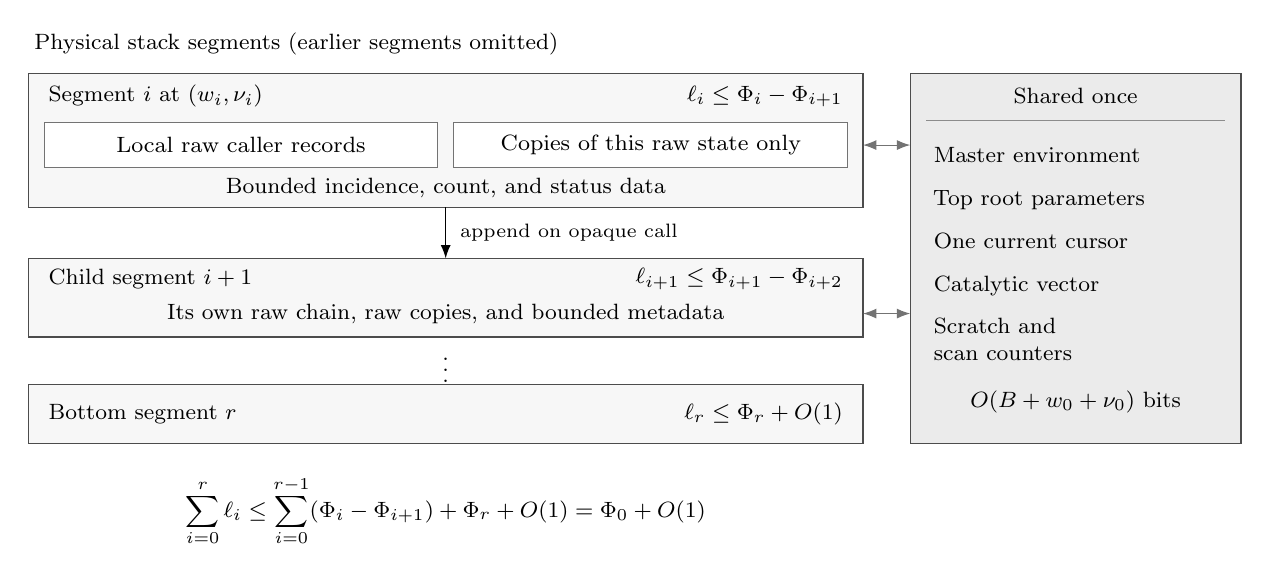
\begin{tikzpicture}[
  x=1cm,y=1cm,
  font=\footnotesize,
  every node/.style={inner sep=2pt},
  segment/.style={draw=black!70,line width=.5pt,fill=black!3},
  raw/.style={draw=black!55,line width=.4pt,fill=white},
  call/.style={-{Latex[length=1.7mm]},line width=.5pt}
]
  \node[anchor=west] at (0,5.62)
    {Physical stack segments \textnormal{(earlier segments omitted)}};

  \draw[segment] (0,3.55) rectangle (10.6,5.25);
  \node[anchor=west] at (.18,4.96) {Segment $i$ at $(w_i,\nu_i)$};
  \node[anchor=east] at (10.42,4.96)
    {$\ell_i\le \Phi_i-\Phi_{i+1}$};
  \draw[raw] (.2,4.05) rectangle (5.2,4.63);
  \node[align=center,text width=4.7cm] at (2.7,4.34)
    {Local raw caller records};
  \draw[raw] (5.4,4.05) rectangle (10.4,4.63);
  \node[align=center,text width=4.7cm] at (7.9,4.34)
    {Copies of this raw state only};
  \node at (5.3,3.79) {Bounded incidence, count, and status data};

  \draw[call] (5.3,3.55) -- (5.3,2.9)
    node[midway,right=3pt,font=\scriptsize] {append on opaque call};
  \draw[segment] (0,1.9) rectangle (10.6,2.9);
  \node[anchor=west] at (.18,2.64) {Child segment $i+1$};
  \node[anchor=east] at (10.42,2.64)
    {$\ell_{i+1}\le \Phi_{i+1}-\Phi_{i+2}$};
  \node at (5.3,2.2)
    {Its own raw chain, raw copies, and bounded metadata};

  \node at (5.3,1.59) {$\vdots$};
  \draw[segment] (0,.55) rectangle (10.6,1.3);
  \node[anchor=west] at (.18,.925) {Bottom segment $r$};
  \node[anchor=east] at (10.42,.925) {$\ell_r\le\Phi_r+O(1)$};

  \draw[draw=black!70,line width=.5pt,fill=black!8]
    (11.2,.55) rectangle (15.4,5.25);
  \node at (13.3,4.96) {Shared once};
  \draw[black!45,line width=.4pt] (11.4,4.65) -- (15.2,4.65);
  \node[align=left,text width=3.6cm] at (13.3,2.96) {
    Master environment\\[6pt]
    Top root parameters\\[6pt]
    One current cursor\\[6pt]
    Catalytic vector\\[6pt]
    Scratch and\\scan counters
  };
  \node[align=center] at (13.3,1.08) {$O(B+w_0+\nu_0)$ bits};
  \draw[<->,>=Latex,black!55,line width=.4pt]
    (10.6,4.34) -- (11.2,4.34);
  \draw[<->,>=Latex,black!55,line width=.4pt]
    (10.6,2.2) -- (11.2,2.2);

  \node[anchor=north] at (5.3,.22) {
    $\displaystyle
      \sum_{i=0}^{r}\ell_i
      \le \sum_{i=0}^{r-1}(\Phi_i-\Phi_{i+1})+\Phi_r+O(1)
      =\Phi_0+O(1)$
  };
\end{tikzpicture}
\caption{Physical stack space, with $\ell_i$ the length of segment $i$
and $\Phi_i=\Phi(w_i,\nu_i)$.  Opaque child work is appended outside raw
copies.  The proved record certificates and local graph bound, with
enlarged $A_{\rm space},D_{\rm space}$, pay for copies and metadata.  Shared facilities are
counted separately.  The displayed copies occur at traversal calls;
older physical segments are not copied into the child.  Ordinary
restoring and numerical segments obey the same difference bound.}
\label{fig:ctrl-space}
\end{figure}


The digit position inequality in \eqref{eq:ctrl-local-bound} gives
\begin{equation}\label{eq:ctrl-clock-invariant}
 \Psi(w_{i+1},\nu_{i+1})\le\Psi(w_i,\nu_i).
\end{equation}
Since $\nu_i\le\Psi(w_i,\nu_i)$, all digit positions are
$O(\nu_{\mathrm{top}}+w_{\mathrm{top}})$.
This also bounds the public scratch calculations in the arithmetic
theorem.  An uncharged full coefficient or cursor copy cannot persist
there: any operand-dependent early word crossing a query was included
in its record certificate, while pure public computations have no
recursive query.  The master environment, cursor, catalyst, scratch
and their global scan counters are single facilities.  Their total
space is $O(B+\nu_{\mathrm{top}}+w_{\mathrm{top}})$.

For exact-stream semantics the induction is valid for each finite
requested digit position, allowing scratch to scale with that digit position.  Every
structural domain uses its fixed finite-margin digit position, so its definition
does not change in this argument.  In particular the integer $N_\nu$ of a
score order statistic or arithmetic operation is always evaluated by its own
place convention, even when used in a request for the next digit.
The actual application has $M_{\mathrm{top}},\nu_{\mathrm{top}}=O(B)$,
and hence all these facilities and active records use $O(B)$ bits.
\end{proof}

\section{Fixed-precision approximation and accepting computations}
\label{sec:conclusion}

We prove Theorem~\ref{thm:fixed-precision}: for each fixed machine
$\mathcal M$ and integer $d\ge1$, a deterministic logarithmic-space
transducer approximates $p_{\mathcal M}(x)$ within $(n+2)^{-d}$ in
polynomial time, with logarithmic output length. The hierarchy gives
a deterministic reward close to the acceptance probability. The
estimator's moment bound gives a majority of accurate environments,
and total evaluation on every environment permits median enumeration.
Section~\ref{sec:deduction} already derives the class equality, promise
separation, and unary-precision approximation from this result.

\subsection{Choosing constants and finite ranges}
\label{subsec:final-constants}

The construction has the following order of choices.
\begin{enumerate}
\item Fix $H,h_0,s=8$ and the fixed number of independent sampling matrices.
The finite-action gap is uniform in every later modulus and bit length.
\item Choose the correction thresholds and cutoff, then the iteration
count $k_*$ from the factorial bound and its resulting uniform
magnitude constants. These estimates hold for every column multiplier
in $[0,1]$.
\item Choose $D_0$ for the entry bound reduction, the routing thresholds,
and the finite ladders of entry and cutoff thresholds. The row-cutoff
rank $K$ can then be chosen from the row-mass bounds alone.
\item Choose the detector rank $J$ large enough for the incidence
bound on extra copies. Choose $R_*$ large enough for overload
detection, and finally the incoming rank $K_c$ large enough for
correction normalization. The earlier row-cutoff choice does not depend
on $K_c$.
\item Fix the bounded-output constant $C_b$, the scale cutoff $c_0$ and
precision coefficient $K_{\rm prec}$, and the prefix mean exponent $B_1$.
Choose the buffer floor and capacity exponents $c_1,c_2$ and the noise
decay $K_n$ so that all buffer sums converge. Choose the rank coefficient
$A_*$ of Equation~\eqref{eq:est-precision} and the walk-length
coefficient $\ell$ sufficiently large for the small constants in the
comparison estimation induction.
\item Fix the crude range and propagation constants, then the block
gain coefficients $D_2,D_1$ and a sufficiently small rational block
width coefficient $\epsilon$. These choices close the coupled
fingerprint induction of Theorem~\ref{thm:fp-estimators}.
\item Choose the fixed operation-stratum and allowance coefficients
and the guard constants in Theorem~\ref{thm:ctrl-realization}.
Their finite enlargement does not alter the analytical tables or
the distribution of the environment.
\item Choose the linear top-budget coefficient, the field-size
exponent, and the minimum padding of $B$.
\end{enumerate}
Within each step only finitely many strict inequalities between
fixed constants are needed. The proofs in the corresponding sections
give these inequalities. In particular, the row rank is fixed before
the incoming rank, the block constants follow the crude error
constants, and the field is chosen after the reachable resource
ranges. There is no dependence of an earlier averaging walk gap on that
last choice.

The coefficient $\epsilon$ in this order is the fixed fingerprint
block-width coefficient. Once it has been chosen, increasing the fixed
linear top budget increases the number of seed blocks but leaves the
averaging walk's gap uniform: all earlier seed bits form one free component in
Lemma~\ref{lem:env-gap}. The storage estimate
\eqref{eq:fp-salt-space} therefore remains $O(B)$.

The allowed family in Section~\ref{subsec:est-tasks} bounds the stage
by $L$, each inherited suffix length by $L-l$ at stage $l$, and every
reciprocal-rate logarithm by
\begin{equation}\label{eq:final-admissible}
HL+C_{\rm rate}(M_{\rm top}-M).
\end{equation}
The closure check after Lemma~\ref{lem:est-paths} verifies both this
finite range and the task-specific inequalities $u\le f$,
$a\le K_f f$ and $t\le a$, including stage resets, preparations,
detectors and reward calls.  The finitely many local operations keep
their task tuple and use the stated widths and fixed subranks.
The controller guards allow these designated executions.

There is consequently a fixed $C_P$ such that a prime
\[
2^{C_PB}\le P\le 2^{C_PB+1}
\]
is larger than all identifiers, makes the radix invertible, and gives
$P2^{-k}\ge1$ for every rate ever requested. Bertrand's postulate
provides such a prime, as it provides the prime of
Lemma~\ref{lem:fp-hash}.
Testing consecutive integers by trial division finds the prime
using $O(B)$ space. The search range and running time are
$2^{O(B)}$. Field arithmetic and fixed-dimensional rank tests also
use $O(B)$ space.

\subsection{A dyadic approximation at the specified start}

\begin{lemma}[Conditioning on one start]\label{lem:final-majority}
Let $V$ be finite, let $W\in[0,1]^V$, and use the sampling matrix
indicators $X_f$ at an admissible rate $f$, with marginal $\pi_f>0$.
Suppose an estimator satisfies
\[
\frac1N\mathbb E\sum_{v\in V}\frac{X_f(v)}f
 |\bar W(v)-W(v)|^8\le C_b^8 2^{-8p}.
\]
For any specified $z\in V$ and every $\eta>0$,
\begin{align}
\mathbb E\bigl[|\bar W(z)-W(z)|^8\mid X_f(z)=1\bigr]
 &\le N\frac f{\pi_f}C_b^8 2^{-8p},
 \label{eq:final-conditional}\\
\Pr\bigl[|\bar W(z)-W(z)|>\eta\mid X_f(z)=1\bigr]
 &\le N\frac f{\pi_f}C_b^8 2^{-8p}\eta^{-8}.
 \label{eq:final-tail}
\end{align}
\end{lemma}

\begin{proof}
Keep only the nonnegative summand at $z$. Since
$\Pr[X_f(z)=1]=\pi_f>0$,
\[
 \frac{\pi_f}{f}
 \mathbb E\bigl[|\bar W(z)-W(z)|^8\mid X_f(z)=1\bigr]
 =\mathbb E\!\left[\frac{X_f(z)}f|\bar W(z)-W(z)|^8\right]
 \le N C_b^8 2^{-8p}.
\]
Dividing by $\pi_f/f$ proves
Equation~\eqref{eq:final-conditional}. In particular, choosing one
specified coordinate costs the factor $N$ from the integrated norm.
Markov's inequality gives Equation~\eqref{eq:final-tail}.
\end{proof}

\begin{proof}[Proof of Theorem~\ref{thm:fixed-precision}]
Apply Lemma~\ref{lem:model-reduction} to $\mathcal M$. Set
\[
 r=d\lceil\log_2(n+2)\rceil,\qquad \Delta=2^{-r},\qquad
 L=\left\lceil\frac{C_0B+r+3}{H-1}\right\rceil,
\]
where $|V_0|\le2^{C_0B}$ is an explicit configuration bound.
Since $d$ is fixed, $r,L=O(B)$. Let $z$ be the copy with every appended digit zero of
the start at stage $L$. Proposition~\ref{prop:hier-reward-target}
gives
\begin{equation}\label{eq:final-hierarchy-accuracy}
 0\le p_{\mathcal M}(x)-W_L(z)\le\Delta/8.
\end{equation}
This bound holds for every acceptance probability. Choose a fixed
$C_N$ large enough to bound all the resulting stage domains by
$N=2^{C_NB}$.

For the final reward task take $a=u=f=b_L$. Its rank satisfies
$i_*=O(L+1)$, and Equation~\eqref{eq:est-precision} reads
\[
 p=M_{\rm top}/K_{\rm prec}-HL-A_*i_*.
\]
By Lemma~\ref{lem:env-ranks}, fix an integer $C_{\rm tail}\ge1$ bounding
$(f/\pi_f)C_b^8$ throughout the admissible range. Choose the fixed
linear coefficient of $M_{\rm top}=O(B)$ large enough that
\begin{equation}\label{eq:final-precision-choice}
 p\ge r+3+\frac{C_NB+\lceil\log_2 C_{\rm tail}\rceil+3}{8}.
\end{equation}
The top-budget and field-size choices in the preceding subsection
allow this enlargement; Equation~\eqref{eq:final-admissible} still
bounds every descendant rate. Theorem~\ref{thm:fp-estimators}
supplies the reward moment estimate. Lemma~\ref{lem:final-majority},
with $\eta=\Delta/8$, now shows that
\begin{equation}\label{eq:final-good-environments}
 \Pr\bigl[|\bar W_L(z)-W_L(z)|>\Delta/8
       \mid X_f(z)=1\bigr]\le1/8.
\end{equation}
Thus the factor $N$ lost on selecting one coordinate has been paid
by the statistical precision. Explicitly, the bound in
Equation~\eqref{eq:final-tail} is at most
\[
 C_{\rm tail}\,2^{C_NB-8p+8r+24}\le 2^{-3},
\]
by Equation~\eqref{eq:final-precision-choice}.

We next turn the estimator values into a finite list of dyadic numbers.
For each master environment, Theorem~\ref{thm:arith-interface}
gives the digits $w_j\in\{-6,\ldots,6\}$ of its one fixed value
$\bar W_L(z)$. Structural choices do not depend on the requested
digit. Put $K=r+6$, compute
\[
 A_\sigma=\sum_{j=0}^{K}w_j2^{K-j},\qquad
 a_\sigma=\min\{2^K,\max\{0,A_\sigma\}\},\qquad
 v_\sigma=a_\sigma2^{-K}.
\]
The integer $A_\sigma$ is obtained by starting at zero and applying
$A\leftarrow2A+w_j$ in order, so it uses $O(K)$ bits.
By Equation~\eqref{eq:arith-tail}, the truncation error is at most
$6\,2^{-K}<\Delta/8$. Clipping cannot increase error relative to
$W_L(z)\in[0,1]$. Equations~\eqref{eq:final-hierarchy-accuracy}
and~\eqref{eq:final-good-environments} imply that, on more than
three quarters of the environments conditioned on $X_f(z)=1$,
\begin{equation}\label{eq:final-dyadic-accuracy}
 |v_\sigma-p_{\mathcal M}(x)|<3\Delta/8.
\end{equation}

Enumerate the conditional law exactly. Enumerate each field-matrix
entry in $\{0,\ldots,P-1\}$ and each raw seed bit string, retaining
precisely those encodings whose positive-degree columns are independent
and for which $X_f(z)=1$. The retained encodings are equally weighted
and give the law in Equation~\eqref{eq:final-good-environments}.
In particular, enumerate the original seed strings, not their reduced
fingerprint parameters. Different raw strings that induce the same
fingerprint remain separate encodings; their multiplicities reproduce
the original probability law. At least one encoding is retained: an independent column tuple
exists, and its independent constant column can place the designated
evaluation in the nonempty retention box. The matrices have fixed
dimensions and $\log P=O(B)$; together with
Equation~\eqref{eq:fp-salt-space}, this gives $O(B)$ bits per master
environment and at most $2^{O(B)}$ encodings to enumerate.

Let $E\ge1$ be the number of retained encodings, found by one pass,
and let $h=\lfloor E/2\rfloor+1$. Binary-search the integer interval
$[0,2^K]$ for the least $a$ such that at least $h$ retained encodings
satisfy $a_\sigma\le a$. Each count is computed by a fresh pass,
recomputing each numerator $a_\sigma$. This finds the upper median
of the finite multiset, including all repetitions. Since more than
three quarters of its members satisfy
Equation~\eqref{eq:final-dyadic-accuracy}, so does its median: fewer than
$E/4$ values can lie below the indicated interval, and fewer than
$E/4$ can lie above it. The algorithm retains only the current count
and search registers; it never stores the multiset.
Output the integers $(a,K)$ representing $z_x=a2^{-K}$. Then
\[
 |z_x-p_{\mathcal M}(x)|<3\Delta/8
       \le(n+2)^{-d}.
\]

We account for the memory held during this computation. The master
environment, current cursor, catalyst, shared scratch, and suspended
controller records together use $O(B)$ bits by
Theorem~\ref{thm:ctrl-realization}, because $M_{\rm top},K=O(B)$.
The outer computation keeps only a fixed number of additional
$O(B)$-bit registers: its top parameters and designated start,
the environment enumeration index, $E$, $h$, the current count,
the two binary-search endpoints and candidate, the digit index,
and the signed numerator accumulator. Each count is bounded by the
number of environment encodings, so it also has $O(B)$ bits.
These outer registers remain live while a digit query runs; in
particular, both its environment-enumeration state and its numerator
accumulator are included. They are present once for the whole
computation, not once per recursive level. Every query terminates on every environment,
including the inaccurate environments, by the same realization
theorem. The output is written only after the median is computed.

Each digit query is a halting deterministic computation with $O(B)$
work bits and physical input heads confined between the real endmarkers.
Counting its finite control, work-tape contents, and all work and input
head positions gives at most $2^{O(B)}$ complete configurations on its
fixed input. A repeated complete configuration would
force a deterministic loop, so totality bounds the query by
$2^{O(B)}$ steps. There are
$2^{O(B)}$ environment encodings, $O(K+1)$ binary-search passes,
and $K+1$ digit queries per numerator. Their product is still
$2^{O(B)}=(n+2)^{O(1)}$. All finite parameters are generated
uniformly, and all constants are fixed for $(\mathcal M,d)$.
\end{proof}

\subsection{Certified accepting computations}

We return to fixed inverse-polynomial accuracy to construct an accepting
computation when the machine's acceptance probability has an
inverse-polynomial lower bound.
For a transducer, the conclusion concerns outputs certified by an
accepting run: its output tape must be write-only, so past emitted
symbols do not influence later transitions.

\begin{corollary}[Certified accepting computations]
\label{cor:certified-search}
Fix a randomized logarithmic-space machine $\mathcal M$ that halts
within a fixed polynomial bound $T(n)\ge1$ on every input and every
coin sequence, and fix an integer $c\ge0$. There is a uniform
deterministic logarithmic-space, polynomial-time transducer that
outputs an accepting computation of $\mathcal M$ whenever
\[
 p_{\mathcal M}(x)\ge(n+2)^{-c}.
\]
On every other input it outputs either an accepting computation or
a failure symbol. If every accepting run of $\mathcal M$ emits a
valid witness for a specified relation, the transducer can instead
output such a witness with the same guarantee.
\end{corollary}

\begin{proof}
Give halted configurations constant self-transitions through time
$T(n)$. A configuration and its elapsed time use $O(\log(n+2))$
bits. There is a fixed randomized logarithmic-space continuation
machine which, on a valid encoding of $(x,v,t)$, starts from
configuration $v$ and simulates the remaining $T(n)-t$ steps with
fresh coins. It checks the fixed work-space box and time bound,
rejecting malformed encodings and any attempted violation. Its
acceptance probability on the reachable configurations is the
continuation value $p_t(v)$, and it has a
polynomial worst-case time bound in its input length.

Write $\gamma=(n+2)^{-c}$. Choose a fixed exponent $d$ large enough
that Theorem~\ref{thm:fixed-precision}, applied to the continuation
machine, approximates every queried value within
$\delta\le\gamma/(8T(n))$. For an explicit choice, fix $C_T\ge1$ and an integer $a_T\ge0$
such that $T(n)\le C_T(n+2)^{a_T}$ for every $n$, and take
\[
 d\ge a_T+c+3+\lceil\log_2 C_T\rceil.
\]
If $m$ is the continuation input length, then $m\ge n$, and
\[
 (m+2)^{-d}\le(n+2)^{-d}
 \le\frac{(n+2)^{-c}}{8C_T(n+2)^{a_T}}
 \le\frac\gamma{8T(n)}.
\]
The extra fields have logarithmic length. We supply them virtually
from saved configuration and time registers, so the approximation
and those registers together use logarithmic space.

Starting at the initial configuration, at each time estimate the
continuation value of every positive-probability successor and
choose one with maximum estimated value, breaking ties by a fixed
port order. Since $p_t(v)$ is the weighted mean of the successor
values, the chosen successor $v'$ satisfies
\[
 p_{t+1}(v')\ge\max_w p_{t+1}(w)-2\delta
                  \ge p_t(v)-2\delta.
\]
On an input satisfying the stated lower bound, after $T(n)$ choices
the terminal continuation value is at least
$\gamma-2T(n)\delta\ge3\gamma/4>0$. A terminal continuation value
is zero or one, so this computation accepts.

First run this construction without writing output. If its terminal
state rejects, output the failure symbol. Otherwise repeat the same
deterministic choices and stream the configurations through the original
first halting state, or the symbols emitted by the simulated transducer.
The artificial self-transitions after halting are omitted from the output.
This second pass follows the same accepting computation. Consequently no rejecting computation
is output, even outside the probability promise.

At any time the current, candidate, and best successor configurations,
the time counter, a constant number of dyadic scores, the virtual
input address, and the approximation workspace occupy a constant
number of $O(\log(n+2))$-bit records. The finite successor lists
have constant size, and there are only $T(n)$ steps in each pass,
so the total running time is polynomial. Each approximation has a
deterministic guarantee at its queried configuration; no simultaneous
accuracy event for all adaptive queries is needed.
\end{proof}

\section{The effective compiler}
\label{sec:compiler}

The probability-approximation theorem fixes the source machine. We now
construct one effective map from source descriptions and supplied
resource bounds to deterministic simulations with explicit bounds.

\begin{theorem}[Effective simulation with explicit bounds]
\label{thm:effective-simulation}
There is a terminating algorithm which, given a finite randomized machine
description ${\mathcal M}$ and positive integers $a,b$, emits a deterministic
machine $\mathcal D_{\mathcal M}$ and positive integers ${K_{\rm space}},{H_{\rm time}},c$ with the following guarantee.
If, on every input of length $n$ and every random tape, ${\mathcal M}$ halts within
$(n+2)^a$ steps, uses at most $b\lceil\log(n+2)\rceil$ work bits, and
has acceptance probability at most $1/3$ on no inputs and at least
$2/3$ on yes inputs, then $\mathcal D_{\mathcal M}$ decides the same language. On each input,
that same execution uses at most ${K_{\rm space}}\log(n+2)$ work bits and
${H_{\rm time}}(n+2)^c$ elementary bit operations.
\end{theorem}

The compiler's own running time need only be finite, and its output
exponent may depend on the source.

We prove Theorem~\ref{thm:effective-simulation} by specializing one
fixed deterministic program. First we construct a randomized interpreter
${\mathcal U}$ that enforces polynomial-time and logarithmic-space bounds on every
input. Theorem~\ref{thm:fixed-precision} supplies a deterministic machine
${\mathcal A_{\rm lib}}$ that separates the inputs on which ${\mathcal U}$ accepts with probability at
least $2/3$ from those on which it accepts with probability at most
$1/3$. Both ${\mathcal U}$ and ${\mathcal A_{\rm lib}}$ are fixed before the compiler receives a source
description ${\mathcal M}$ and bounds $a,b$.

When the source satisfies its supplied resource bounds, padding places
each encoded computation within ${\mathcal U}$'s caps without changing its
acceptance probability. The generated machine runs ${\mathcal A_{\rm lib}}$ on that padded input, generating each requested
symbol from the real input. We then compute the output bounds ${K_{\rm space}},{H_{\rm time}},c$
from the generated finite transition table and the fixed library data.

Universal deterministic estimation has a substantial antecedent in
Pyne, Raz and Zhan~\cite[full version, Theorem~5.1]{PyneRazZhan2023}.
They construct one deterministic algorithm that, on input $(1^n,\mathcal B)$
with $n\ge1$ and $\mathcal B$ an ordered branching program of length
and width at most $n$, approximates its acceptance probability to error less than
$1/n$. For every space-constructible $S(n)\ge\log n$, this single
algorithm uses $O(S(n))$ space exactly when
$\mathsf{prBPL}\subseteq\mathsf{SPACE}[O(S(n))]$.
Here the preceding sections establish the separator used by one fixed
library, and we compute explicit resource bounds for its source-specific
specialization.

All quantities in this section are local to the compiler construction.
In particular, ${P_{\rm pad}}$ is a padding exponent, $d_{\mathrm{code}}$ is a program
length, $\ell_n=\lceil\log_2(n+2)\rceil$, and $N_{\mathrm{pad}}$ is a virtual
input length.  They do not denote the statistical budgets, field modulus,
or domain sizes used in the preceding sections.  We use the usual
counted-cell convention for work tapes: traversed writable cells count
toward space, whether or not they contain a nonblank symbol.  The finite
control and the read-only input have their standard treatment.

\subsection{One fixed interpreter with enforced resource bounds}
\label{subsec:compiler-interpreter}

Fix a binary coding of ordinary finite transition lists.  One concrete
choice uses a fixed record grammar and the field encoding
$w\mapsto 1^{|w|}0w$.  Lists specify the finite state set, tape and
alphabet declarations, initial and halting states, blanks and endmarkers,
and transition records.  A transition record lists its tested state,
scanned symbols and coin pattern, followed by its next state, written
symbols and local head movements.  The grammar has fixed nesting depth;
its fields are actual listed data, not recursively executable descriptions.
State and symbol IDs are canonical binary integers used only as names.
The first matching transition is
used; a missing transition causes rejection.  Wildcards for ignored coins
can equivalently be expanded into a finite explicit list.

Write $z$ for a program in this coding and
$d_{\mathrm{code}}=|z|\ge1$.  The coding permits at most
$d_{\mathrm{code}}$ work tapes and a block of at most
$d_{\mathrm{code}}$ fresh fair bits per simulated transition.  Every ID
has at most $d_{\mathrm{code}}$ bits.  A harmless padding field can enlarge
the program to meet these inequalities.  All tape movements are local.
Work coordinates are measured from their initial origins; the ordinary
model has one input head and one head per work tape.  For a source input
$x$ of length $n$, let $E_{d_{\mathrm{code}}}(x)$ encode each of its
symbols by its ID padded to exactly $d_{\mathrm{code}}$ bits.

\paragraph{Preserving the supplied source bounds.}
An ordinary source machine ${\mathcal M}$ can be converted effectively to this format
by renaming its states and symbols and listing its transitions.  Its tapes
are represented directly, so a source transition retains its work writes
and head movements and counts as one interpreted transition.  The
conversion does not pass through a slower single-tape simulation.

Under the optional one-way read-only random-tape convention, the source
may reuse its current random bit. Store a cached bit and a validity flag
in finite control, initially invalid.
At each transition obtain one fresh bit.  Use it if the cache is invalid;
otherwise use the cached bit and discard the fresh one.  Execute the
source transition, then retain the used bit if the random head stayed
and invalidate the cache if it advanced.  This samples a newly visited
random cell lazily on its next use.  It preserves the joint distribution
of the source run and needs no initialization transition.  An initially
halting state is recognized before the first transition.  The same
argument uses a fixed finite block for a convention allowing finitely
many fresh bits per elementary transition, discarding unused bits.
The finite cache changes neither counted work space nor the number of
source transitions.  Thus the supplied parameters $a,b$ remain valid;
only the static description length can increase.

\begin{lemma}[A total resource-capped interpreter]
\label{lem:compiler-interpreter}
There is one fixed randomized Turing machine ${\mathcal U}$ with polynomial
worst-case running time and $O(\log(m+2))$ counted work bits on every
binary input of length $m$, with the following behavior.
Set
\begin{equation}\label{eq:compiler-interpreter-cap}
 \ell_m^{\rm in}=\lceil\log_2(m+2)\rceil,
 \qquad
 R(m,d_{\mathrm{code}})
   =\left\lfloor\frac{\ell_m^{\rm in}}
       {100(d_{\mathrm{code}}+1)^3}\right\rfloor.
\end{equation}
On an input with prefix
\begin{equation}\label{eq:compiler-prefix}
  1^{d_{\mathrm{code}}}0\,z\,1^n0\,
  E_{d_{\mathrm{code}}}(x),
\end{equation}
it first requires $1\le d_{\mathrm{code}}\le\ell_m^{\rm in}$ and
$R(m,d_{\mathrm{code}})\ge1$.  It then simulates the encoded machine
for at most $m$ transitions, allowing each counted work tape only
coordinates in $[-R,R]$.  It rejects malformed data, a requested move
outside these bounds, or failure to halt by the end of the transition
budget.  Otherwise it returns the encoded machine's decision.  The
suffix after the complete prefix has no parsing significance.
\end{lemma}

\begin{proof}
Count $m$ before interpreting the prefix.  Scan the unary code-length
header with a bounded counter, rejecting if its length exceeds
$\ell_m^{\rm in}$ or the required delimiter is absent.  Check the two
eligibility conditions before copying $z$ or allocating simulation
storage.  Then verify that the following $d_{\mathrm{code}}$ code bits,
the unary data-length header, and the required data bits are present.
The parsed $n$ is at most $m$, and
$d_{\mathrm{code}}n\le\ell_m^{\rm in} m$, so even size calculations preceding
a failed length check use only $O(\ell_m^{\rm in})$ bits.  List counts, ID
lengths, tape declarations, and movements are checked against the actual
code and the stated bounds before any loops or allocations using them.
There is no enumeration of an implicit domain of symbol or state names.

Store the encoded tapes sequentially on a fixed number of real work
tapes of ${\mathcal U}$.  At most $d_{\mathrm{code}}$ strips, each with $2R+1$
cells of $d_{\mathrm{code}}$ bits, require
\begin{equation}\label{eq:compiler-interpreter-space}
 d_{\mathrm{code}}^2(2R+1)=O(\ell_m^{\rm in})
\end{equation}
bits.  Indeed, eligibility gives
$d_{\mathrm{code}}^3\le\ell_m^{\rm in}$ and
$d_{\mathrm{code}}^2R\le\ell_m^{\rm in}$.
The copied program, current state, scanned and written symbol tuples,
coin block, strip coordinates, step counter, and parsing scratch fit
simultaneously in $O(\ell_m^{\rm in})$ bits.  A single simulated input-head
coordinate has magnitude $O(m)$ by the transition cap and therefore
also uses $O(\ell_m^{\rm in})$ bits.  Read the corresponding source symbol
by rescanning the encoded data, supplying the appropriate markers or
off-data blanks according to the encoded input-tape convention.

All routines are bounded scans and ordinary binary arithmetic.  They
iterate over actual code positions, input positions, a bounded tape/head
list, strip positions, and bit positions, with a fixed nesting depth.
Each range is polynomially bounded in $m+2$; binary arithmetic is
implemented by bit scans, not unit-cost operations on growing words.
Matching a listed transition, fetching input symbols, updating the
strips, and obtaining its finite coin block therefore take polynomial
time in $m+2$, with one fixed exponent determined by these routines.
The same bounds hold when a check fails.  There are at most $m$
interpreted transitions.  Checking the initial halting state and the
state reached by the last permitted transition gives the asserted
total behavior, including $m=0$.  The resulting fixed ${\mathcal U}$ has the
required polynomial worst-case time on every random tape.
\end{proof}

No bounded-error language promise is asserted for ${\mathcal U}$ on arbitrary
inputs.  Its acceptance probability may lie between $1/3$ and $2/3$.
This is why we use probability approximation rather than a bare
language-class containment.

\begin{remark}[Optional head conventions]
The construction also applies when the fixed coding and ${\mathcal U}$ are chosen
to allow at most $d_{\mathrm{code}}$ heads per tape, with the usual common
initial origin. These conventions are fixed before choosing the
deterministic library in Section~\ref{subsec:compiler-library}.
There are then at most $d_{\mathrm{code}}^2$ work-head coordinates and
scanned symbols.  Their storage is bounded by
\[
 O\bigl(d_{\mathrm{code}}^2\log(2R+1)
          +d_{\mathrm{code}}^3\bigr)=O(\ell_m^{\rm in}).
\]
For multiple input heads, or an optional entirely blank tape whose
cells are not charged, use signed $R$-bit coordinates and reject on
overflow.  At most $d_{\mathrm{code}}^2$ such coordinates still cost
$O(d_{\mathrm{code}}^2R)$ bits.  These optional conventions do not
change the interpreter's bounds. The instances in
Section~\ref{subsec:compiler-padding} never overflow those coordinates
by Equation~\eqref{eq:compiler-strip-slack}.
\end{remark}

\subsection{Fixing one deterministic library}
\label{subsec:compiler-library}

Apply Theorem~\ref{thm:fixed-precision} to the fixed machine ${\mathcal U}$ and
accuracy exponent $3$, and compare its dyadic answer with $1/2$.
The error on an input of length $m$ is at most
$(m+2)^{-3}\le1/8$.  Hence the resulting deterministic machine accepts
whenever $\Pr[{\mathcal U}\text{ accepts}]\ge2/3$ and rejects whenever that
probability is at most $1/3$, since
\[
 \frac13+\frac18=\frac{11}{24}<\frac12
   <\frac{13}{24}=\frac23-\frac18.
\]
It halts on every input, including inputs between the two thresholds,
as also stated in Corollary~\ref{cor:promise-bpl}.  Its logarithmic
space bound counts all simultaneously live work in the approximation
algorithm.  Store the $O(\log(m+2))$-bit dyadic output in work space
for the threshold test.

We fix this library once in the following convenient form.  It is an
ordinary finite-tape deterministic decision machine ${\mathcal A_{\rm lib}}$ with one input
head confined to the endmarked input, initially at its left endmarker,
such that every work head stays in
\begin{equation}\label{eq:compiler-library-box}
 [-(\ell_m^{\rm in}+1),\ell_m^{\rm in}+1]
\end{equation}
relative to its origin.  To obtain this form, first consolidate any
input heads by keeping their coordinates in logarithmic work space
and scanning for each read.  Even an off-data coordinate under an
unbounded-input convention has logarithmic length because the original
library has polynomial running time.  A fixed change of initial control
state handles its input-head start convention.

Next choose an integer $w$ at least a coefficient bounding each counted
work head's distance from its origin by $w\ell_m^{\rm in}$.  Such one fixed
$w$ exists from the logarithmic bound, enlarged if necessary for the
finitely many small lengths.  Group consecutive work cells into blocks
of width $w$, storing within-block offsets in finite control.  The
resulting finite alphabet and finite transition list realize
Equation~\eqref{eq:compiler-library-box}, also for two-sided tapes.
All symbol widths will be charged in bits below; grouping only exposes
a uniform address bound and gives no uncharged bit compression.

This choice of ${\mathcal A_{\rm lib}}$, including its one blocking width, precedes every
compiler input.  More formally, the remaining construction is a
computable syntactic function of a finite library list and
$({\mathcal M},a,b)$.  Fixing one valid finite list yields one ordinary
computable compiler on all those source inputs.  The existence
of the fixed list was proved by Theorem~\ref{thm:fixed-precision};
no constant is selected as a noncomputable function of the source
machine or its ordinary input.

The fixed finite data are the program grammar, the transition list of
${\mathcal A_{\rm lib}}$ with its blocked work alphabets and head conventions, and the
finite callback templates described below. The construction constants,
cutoffs, generator choices and finite instruction routines used by the
separator are included in that list. Its blocking width is fixed at
the same time. These are data specifying one compiler; subsequent
source-dependent integers are computed from these data and the supplied
$({\mathcal M},a,b)$.

\subsection{Padding and exact preservation of acceptance probability}
\label{subsec:compiler-padding}

Given the source description and its supplied positive integers $a,b$,
construct $z$ as above and compute
\begin{equation}\label{eq:compiler-padding}
 \begin{split}
 {P_{\rm pad}}&=1000(d_{\mathrm{code}}+2)^4(a+b+2),\\
 \ell_n&=\lceil\log_2(n+2)\rceil,
 \qquad N_{\mathrm{pad}}=2^{P_{\rm pad}\ell_n}.
 \end{split}
\end{equation}
The generated machine will run ${\mathcal A_{\rm lib}}$ on a virtual binary input
$y_x$ of length $N_{\mathrm{pad}}$ whose prefix is
Equation~\eqref{eq:compiler-prefix} and whose remaining bits are zero.
Its prefix length is exactly
\begin{equation}\label{eq:compiler-prefix-length}
 L_{\mathrm{pre}}
 =(d_{\mathrm{code}}+1)+d_{\mathrm{code}}+(n+1)
       +d_{\mathrm{code}}n
 =(d_{\mathrm{code}}+1)(n+2).
\end{equation}
Since $\ell_n\ge1$, $2^{\ell_n}\ge n+2$, and
$2^{{P_{\rm pad}}-1}\ge d_{\mathrm{code}}+1$, this length is at most
$N_{\mathrm{pad}}$.  The interpreter's length parameter is
\begin{equation}\label{eq:compiler-padded-log}
 \ell_{\mathrm{pad}}
 :=\ell_{N_{\mathrm{pad}}}^{\rm in}=P_{\rm pad}\ell_n+1.
\end{equation}

All eligibility checks pass.  In particular,
\[
 \frac{{P_{\rm pad}}}{100(d_{\mathrm{code}}+1)^3}
 =10\frac{(d_{\mathrm{code}}+2)^4}
          {(d_{\mathrm{code}}+1)^3}(a+b+2)
 \ge30(a+b+2),
\]
so
\begin{equation}\label{eq:compiler-strip-slack}
 R(N_{\mathrm{pad}},d_{\mathrm{code}})
 \ge30(a+b+2)\ell_n-1\ge(a+b)\ell_n+4.
\end{equation}
Also ${P_{\rm pad}}>a$, whence
$(n+2)^a\le2^{a\ell_n}<N_{\mathrm{pad}}$.
Local motion from an initial work origin to a cell entails visiting
the intervening counted cells.  The source bound of $b\ell_n$ work bits
therefore places every source work cell in the allocated strip;
the slack in Equation~\eqref{eq:compiler-strip-slack} also covers a final
one-cell move.  This uses the source's original cell costs, each at
least one bit, and does not charge it for the larger interpreter IDs.

Under the optional head conventions, local motion bounds an input or
uncharged blank-tape coordinate by the source time, up to the fixed
endmarker offset.  Its signed encoding fits because $R\ge a\ell_n+4$.

Consequently no resource cutoff changes a promised source run, and
\begin{equation}\label{eq:compiler-exact-probability}
 \Pr[{\mathcal U}(y_x)\text{ accepts}]=\Pr[{\mathcal M}(x)\text{ accepts}].
\end{equation}
The decision of ${\mathcal A_{\rm lib}}(y_x)$ is therefore the decision required for the source language.
Although $N_{\mathrm{pad}}$ is given exponentially, it is at most
$(n+2)^{2{P_{\rm pad}}}$ for the fixed source.  More importantly, it need never
be written as an input string.



Figure~\ref{fig:compiler-padding} shows how the generated machine supplies
the virtual input requested by ${\mathcal A_{\rm lib}}$. The library's work tapes remain live
while the callback scans the real input; the resource bound below counts
the library and callback storage simultaneously.

\begin{figure}[tb]
 \centering
 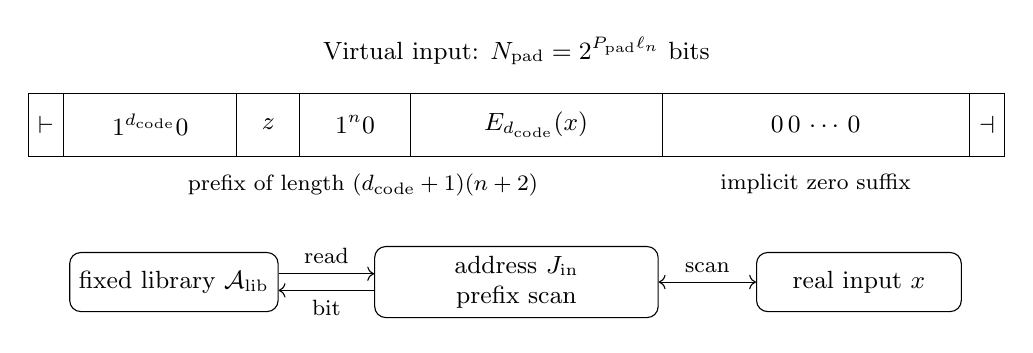
\begin{tikzpicture}[x=1cm,y=1cm,font=\small]
  \draw (0,0) rectangle (12.4,0.8);
  \draw (0.45,0) -- (0.45,0.8);
  \draw (2.65,0) -- (2.65,0.8);
  \draw (3.45,0) -- (3.45,0.8);
  \draw (4.85,0) -- (4.85,0.8);
  \draw (8.05,0) -- (8.05,0.8);
  \draw (11.95,0) -- (11.95,0.8);
  \node at (0.225,0.4) {$\vdash$};
  \node at (1.55,0.4) {$1^{d_{\mathrm{code}}}0$};
  \node at (3.05,0.4) {$z$};
  \node at (4.15,0.4) {$1^n0$};
  \node at (6.45,0.4) {$E_{d_{\mathrm{code}}}(x)$};
  \node at (10,0.4) {$0\,0\,\cdots\,0$};
  \node at (12.175,0.4) {$\dashv$};
  \node[anchor=south] at (6.2,1.03)
    {Virtual input: $N_{\mathrm{pad}}=2^{P_{\rm pad}\ell_n}$ bits};
  \node[anchor=north,font=\footnotesize] at (4.25,-0.1)
    {prefix of length $(d_{\mathrm{code}}+1)(n+2)$};
  \node[anchor=north,font=\footnotesize] at (10,-0.1)
    {implicit zero suffix};
  \node[draw,rounded corners,align=center,minimum width=2.6cm,
        minimum height=0.75cm] (library) at (1.85,-1.6)
    {fixed library ${\mathcal A_{\rm lib}}$};
  \node[draw,rounded corners,align=center,minimum width=3.6cm,
        minimum height=0.75cm] (callback) at (6.2,-1.6)
    {address ${J_{\rm in}}$\\prefix scan};
  \node[draw,rounded corners,align=center,minimum width=2.6cm,
        minimum height=0.75cm] (realinput) at (10.55,-1.6)
    {real input $x$};
  \draw[->] ([yshift=3pt]library.east) -- ([yshift=3pt]callback.west)
    node[midway,above,font=\footnotesize] {read};
  \draw[->] ([yshift=-3pt]callback.west) -- ([yshift=-3pt]library.east)
    node[midway,below,font=\footnotesize] {bit};
  \draw[<->] (callback.east) -- (realinput.west)
    node[midway,above,font=\footnotesize] {scan};
\end{tikzpicture}

 \caption{The fixed library reads the padded input at virtual input-head
 address ${J_{\rm in}}$ through a callback.
 The callback regenerates prefix symbols from the real input and returns
 zero for an address in the padding interval.}
 \label{fig:compiler-padding}
\end{figure}

\subsection{Compiling the virtual input operations}
\label{subsec:compiler-callback}

Inline the finite transition list of ${\mathcal A_{\rm lib}}$, giving it its own work tapes.
The generated machine ${\mathcal D_{\mathcal M}}$ suspends its library control state in finite
control during an input operation.  Four auxiliary binary words suffice:
the length count $n+1$, the virtual right-endmarker address
$N_{\mathrm{pad}}+1$, the virtual input-head position ${J_{\rm in}}$, and a prefix
position ${J_{\rm pre}}$.  Each has a separate tape, with origin and termination
marks and digits in low-end-first order.

Initialize the length count to one and increment it once per real input
symbol.  Its bit length is exactly
\begin{equation}\label{eq:compiler-bitlength}
 \operatorname{bitlength}(n+1)
   =\lfloor\log_2(n+1)\rfloor+1
   =\lceil\log_2(n+2)\rceil=\ell_n
 \qquad(n\ge0).
\end{equation}
For every bit place in that count, write ${P_{\rm pad}}$ zero bits on the bound tape,
then append a one.  This produces the low-end-first representation of
$2^{P_{\rm pad}\ell_n}=N_{\mathrm{pad}}$; increment it to obtain
$N_{\mathrm{pad}}+1$.  The repetition of ${P_{\rm pad}}$ is hardwired finite control.
Initially set ${J_{\rm in}}=0$, the library's left-endmarker position.

At a virtual read, first test ${J_{\rm in}}=0$ and ${J_{\rm in}}=N_{\mathrm{pad}}+1$ and return
the corresponding endmarker.  Otherwise initialize ${J_{\rm pre}}=1$ and regenerate
the prefix in its natural order:
\begin{enumerate}
 \item emit the fixed string $1^{d_{\mathrm{code}}}0z$;
 \item scan $x$, emitting one $1$ per symbol, and then emit $0$;
 \item rewind and scan $x$ again, emitting each fixed-width symbol code
       in $E_{d_{\mathrm{code}}}(x)$.
\end{enumerate}
Here ``emit'' means compare the current ${J_{\rm pre}}$ with ${J_{\rm in}}$, return the bit
if they agree, and otherwise increment ${J_{\rm pre}}$ and continue.  If the scan
finishes without a match, return zero.  The strings $z$, the integer
$d_{\mathrm{code}}$, symbol codes and emission phases are fixed in
the generated control.  The real input head is rewound by scanning to
its endmarker, without storing its position.  In particular,
${J_{\rm in}}=N_{\mathrm{pad}}+1$ is answered before regeneration, while a padding
address such as ${J_{\rm in}}=N_{\mathrm{pad}}$ returns zero after the finite
prefix scan.  The largest prefix counter value is
$L_{\mathrm{pre}}+1\le N_{\mathrm{pad}}+1$.

For explicit counter routines, an increment uses a finite carry flag.
Compare two low-end-first words by scanning both, retaining only a
finite comparison flag that is overwritten by each higher differing
bit.  After one terminator, treat its later bits as zero using a finite
``ended'' flag.  Rewind each tape to its origin mark afterward.  Zeroing
and copying are likewise bounded bit scans.  No growing arithmetic
register beyond the named words is required.  All words have at most
$P_{\rm pad}\ell_n+2$ bits; including delimiters and rewinds, their heads need visit
only positions through $P_{\rm pad}\ell_n+10$.

After the callback, perform the indicated library transition and update
${J_{\rm in}}$ in place for its input-head motion.  The library's work heads and
contents are untouched by the callback.  Its state, the returned input
symbol, and any step-local scanned tuple are fixed finite-control data.
The callback does not invoke ${\mathcal A_{\rm lib}}$ recursively or maintain a stack of
callbacks.  The real input head stays between its real endmarkers.

Every listed routine terminates.  For example, a complete regeneration
uses at most $L_{\mathrm{pre}}$ emissions, each with an
$O(P_{\rm pad}\ell_n+1)$-bit comparison and increment, together with two real-input
scans.  Initialization makes $n$ increments and writes $P_{\rm pad}\ell_n+1$ bound
bits.  These observations give direct polynomial bounds for the
auxiliary operations.  The whole simulation halts because ${\mathcal A_{\rm lib}}$ is total.
Its more uniform explicit time bound, including every such operation,
is derived next from the complete configurations of this same machine.

All the above instructions can be generated as finite transition tables,
unrolling fixed repetitions and strings if necessary.  Formation of the
source list, the integer ${P_{\rm pad}}$, and this transition table is a finite
effective process.  Syntactically invalid compiler inputs may be assigned
a fixed default output; correctness is required on the stipulated class.
The generated simulation is total and obeys the bounds below even when
the supplied source promises fail; those promises are used to establish
that its decision agrees with the source.

\subsection{Explicit simultaneous bounds}
\label{subsec:compiler-bounds}

Use the finite-alphabet description just constructed to compute ${n_{\rm tapes}}$, its
number of work tapes; ${g_{\rm alph}}\ge2$, the maximum of two and its work alphabet
sizes, including all blank, origin and termination symbols; and $q_D$,
its number of states, including callback phases.  Let ${u_{\rm code}}\ge1$ dominate
its explicit transition-table bit length, all alphabet sizes (including
the input alphabet), the number of states, and the number of tapes.
Padding this integer is effective.  Return the positive integer bounds
\begin{equation}\label{eq:compiler-output-bounds}
 \begin{split}
 \rho_{\rm tape}&=100({P_{\rm pad}}+2),\qquad
 {S_{\rm code}}=1+({n_{\rm tapes}}+1)(2\rho_{\rm tape}+1)({g_{\rm alph}}+2),\\
 {K_{\rm space}}&=4{S_{\rm code}},\qquad c=2{S_{\rm code}}+1,\qquad
 {H_{\rm time}}=2^{({u_{\rm code}}+100)^2}(q_D+1).
 \end{split}
\end{equation}
These depend on the fixed source and the fixed library, and are computed
from finite syntax.  They have no dependence on $n$ or $x$.

\paragraph{All live work bits.}
Every work head stays in
$[-\rho_{\rm tape} \ell_n,\rho_{\rm tape} \ell_n]$.  For a library tape this follows from
Equations~\eqref{eq:compiler-library-box} and
\eqref{eq:compiler-padded-log}, since
$\ell_{\mathrm{pad}}+1=P_{\rm pad}\ell_n+2\le\rho_{\rm tape} \ell_n$.
For an auxiliary tape it follows from
$P_{\rm pad}\ell_n+10\le\rho_{\rm tape} \ell_n$, using $\ell_n\ge1$.
Thus the library's live data and all callback data satisfy the same
bound at the same time.  Encoding a work alphabet of size $g_i$ in
$\max\{1,\lceil\log_2 g_i\rceil\}\le {g_{\rm alph}}$ bits per symbol bounds
their total data by
\begin{equation}\label{eq:compiler-space-bound}
 {n_{\rm tapes}}(2\rho_{\rm tape} \ell_n+1){g_{\rm alph}}\le S_{\rm code}\ell_n.
\end{equation}
Even twice this quantity satisfies the stronger logarithmic bound: with
$L_n=\log_2(n+2)\ge1$ we have $\ell_n\le2L_n$ and
\[
 2S_{\rm code}\ell_n\le4S_{\rm code}L_n={K_{\rm space}} L_n.
\]

\paragraph{All finite-alphabet transitions.}
For a fixed real input $x$, a complete configuration is specified by
the state, the real input-head position, all work-head positions, and
all work symbols in the stated intervals.  Everything outside these
intervals remains at its initial value.  There are at most
\begin{equation}\label{eq:compiler-configurations}
 q_D(n+2)(2\rho_{\rm tape} \ell_n+1)^{n_{\rm tapes}}
       {g_{\rm alph}}^{{n_{\rm tapes}}(2\rho_{\rm tape} \ell_n+1)}
 \le q_D(n+2)2^{S_{\rm code}\ell_n}
 \le q_D(n+2)^c
\end{equation}
such configurations.  For the first inequality use
\[
 2\rho_{\rm tape} \ell_n+1\le(2\rho_{\rm tape}+1)\ell_n,
 \quad \log_2{g_{\rm alph}}\le {g_{\rm alph}},
 \quad \log_2(2\rho_{\rm tape} \ell_n+1)\le(2\rho_{\rm tape}+1)\ell_n;
\]
the second uses $\ell_n\le2\log_2(n+2)$ and $c=2{S_{\rm code}}+1$.
A deterministic halting computation cannot repeat a complete
configuration.  Therefore Equation~\eqref{eq:compiler-configurations}
bounds its total transitions, including initialization, counter
arithmetic, every regenerated input bit, and every library transition.
The virtual head position is already in the counted word ${J_{\rm in}}$; it is
not an additional uncounted configuration component.

\paragraph{Elementary bit operations.}
The preceding count refers to ordinary finite-alphabet transitions.
To charge them in bits, encode each work symbol by a fixed-width block,
mapping blank to the all-zero block.  Read and write within the current
block, return to its first bit, and move to the first bit of the target
block.  Within-block phases and scanned finite tuples are stored in
finite control.  No per-block writable delimiter is needed, and these
operations visit only blocks whose macro positions occur in the proved
work intervals.  Existing origin and termination symbols have already
been included in ${g_{\rm alph}}$.  Thus the block implementation obeys the bit-space
estimate above; the factor two also allows the usual blank/bit tape
convention.  Input-symbol access has fixed width and is covered by the
same finite description parameter ${u_{\rm code}}$.

There are at most ${u_{\rm code}}+1$ scanned symbols of at most ${u_{\rm code}}$ bits each.
An explicit sequential comparison against at most ${u_{\rm code}}$ transition rows,
followed by the fixed-width reads, writes and moves, uses at most a
fixed polynomial in ${u_{\rm code}}+1$ bit actions per transition.  For example,
the deliberately loose bound $100({u_{\rm code}}+1)^8$ suffices for these scans
and comparisons, with all temporary phase and symbol information in
finite control.  It is dominated, for ${u_{\rm code}}\ge1$, by
\[
 100({u_{\rm code}}+1)^8\le2^{({u_{\rm code}}+100)^2}.
\]
The binary microcode may have more states than $q_D$, but no new
configuration count is needed: multiply the number of original
transitions by this per-transition bit cost.  Equations~\eqref{eq:compiler-output-bounds}
and~\eqref{eq:compiler-configurations} give the simultaneous bound
\begin{equation}\label{eq:compiler-time-bound}
 \operatorname{time}_{\mathrm{bit}}({\mathcal D_{\mathcal M}},x)
 \le {H_{\rm time}}(n+2)^c.
\end{equation}
No growing-word arithmetic is charged as a single elementary bit action.

\begin{proof}[Completion of the proof of Theorem~\ref{thm:effective-simulation}]
The compiler returns the described machine ${\mathcal D_{\mathcal M}}$ and the integers
${K_{\rm space}},{H_{\rm time}},c$ in Equation~\eqref{eq:compiler-output-bounds}.  Its finite
syntactic construction terminates.  On every promised source input,
Equation~\eqref{eq:compiler-exact-probability} and the fixed separator's
threshold guarantee give the correct decision.  The totality of ${\mathcal A_{\rm lib}}$
and the finite callback loops prove halting.  Equations~\eqref{eq:compiler-space-bound}
and~\eqref{eq:compiler-time-bound} give at most ${K_{\rm space}}\log_2(n+2)$
work bits and ${H_{\rm time}}(n+2)^c$ bit operations for this same machine.

All claims include $n=0$: then $\ell_n=1$, the real-input scans are empty,
the count $n+1=1$ has one bit, and every displayed padding, strip,
space, and time inequality remains valid.  The library's grouping
width already includes its finitely many small-length exceptions.
All construction constants are fixed before the ordinary input is read.

The work and time internal to probability approximation---environment
enumeration, numerical digits, recursive interfaces, recomputation,
and precision management---belong to the one complete library machine
proved in Theorem~\ref{thm:fixed-precision}.  Its tapes remain counted
throughout virtualization.  The compiler adds only the exact input
operations analyzed here.  Configuration counting gives polynomial time because this
entire deterministic machine uses exact logarithmic space.
\end{proof}


\bibliographystyle{plain}
\bibliography{references}
\end{document}
